\documentclass[a4paper]{report}
\usepackage{setspace}
\usepackage{subcaption}

\pagestyle{plain}
\usepackage{amssymb,graphicx,color}
\usepackage{amsfonts}
\usepackage{latexsym}
\usepackage{amsmath}
\usepackage[a4paper, margin = 3cm, bottom = 2.5cm]{geometry}

\usepackage{float}

\usepackage{pgfplots}
\pgfplotsset{compat=1.18}

\usepackage{tikz}
\usetikzlibrary{arrows.meta}

\usepackage{amsmath}
\usepackage{algorithm}
\usepackage[noend]{algpseudocode}

\usepackage{makecell}

\newtheorem{theorem}{THEOREM}
\newtheorem{lemma}[theorem]{LEMMA}
\newtheorem{corollary}[theorem]{COROLLARY}
\newtheorem{proposition}[theorem]{PROPOSITION}
\newtheorem{remark}[theorem]{REMARK}
\newtheorem{definition}[theorem]{DEFINITION}
\newtheorem{fact}[theorem]{FACT}

\newtheorem{problem}[theorem]{PROBLEM}
\newtheorem{exercise}[theorem]{EXERCISE}
\def \set#1{\{#1\} }

\newenvironment{proof}{
PROOF:
\begin{quotation}}{
$\Box$ \end{quotation}}



\newcommand{\nats}{\mbox{\( \mathbb N \)}}
\newcommand{\rat}{\mbox{\(\mathbb Q\)}}
\newcommand{\rats}{\mbox{\(\mathbb Q\)}}
\newcommand{\reals}{\mbox{\(\mathbb R\)}}
\newcommand{\ints}{\mbox{\(\mathbb Z\)}}

%%%%%%%%%%%%%%%%%%%%%%%%%%

\pagenumbering{roman}

\title{{\vspace{-14em} 
\includegraphics[scale=0.4]{images/ucl_logo.png}}\\
{{\Huge Investigating the use of Decentralised Reinforcement Learning Algorithms in Traffic Environments}}\\
% {\large Optional Subtitle}\\
}
\date{Submission date: Day April 2026}
\author{23091179\thanks{
{\bf Disclaimer:}
This report is submitted as part requirement for the BSc Degree in Computer Science at UCL. It is
substantially the result of my own work except where explicitly indicated in the text.
The report may be freely copied and distributed provided the source is explicitly acknowledged.
\newline  %% \\ messes it up
}
\\ \\
BSc Computer Science\\ \\
Supervisor: Prof. Graham Roberts}



\begin{document}
 
\onehalfspacing
\maketitle

\chapter*{\centering\large Acknowledgements}
\vspace{-1cm}
I would like to extend my gratitude to my supervisor Prof. Graham Roberts for his unwavering support during my final year of study, his patience, and motivation. The numerous meetings and e-mail communications throughout the course of the year have been greatly appreciated.

Thank you to the team at the German Aerospace Center (DLR) for the free and open source SUMO traffic simulation suite and documentation used heavily in this dissertation.

And, of course, thank you to my family and everyone else (you know who you are!) for the support throughout my life, particularly during these last few years of education.

\chapter*{\centering\large Abstract}
\vspace{-1cm}
This project explores the use of intelligent agents for controlling traffic light systems in order to optimise vehicle and pedestrian throughput. Specifically, we explore a family of reinforcement learning algorithms which are decentralised in that each traffic light system runs its own algorithm; we seek to answer the question of whether these agents can provide a non-insignificant improvement upon existing systems.

We begin with a review of existing traffic light systems, motivating the need for agents. Following this, we see how detailed environments for conducting traffic experiments can be built using the SUMO traffic simulation suite, including synthesised traffic of varying conditions. Finally, we incrementally build three Q-learning-based algorithms from scratch, justifying each along the way.

The final result reached is a system consisting of multiple agents capable of independently controlling traffic lights and sharing state between one another. The benefits over traditional traffic light systems are provisionally confirmed in numerous evaluation configurations, however there were also a number of caveats unveiled not to be ignored.\\ \\

\begin{figure}[H]
    \centering
    \begin{subfigure}{0.48\textwidth}
        \centering
        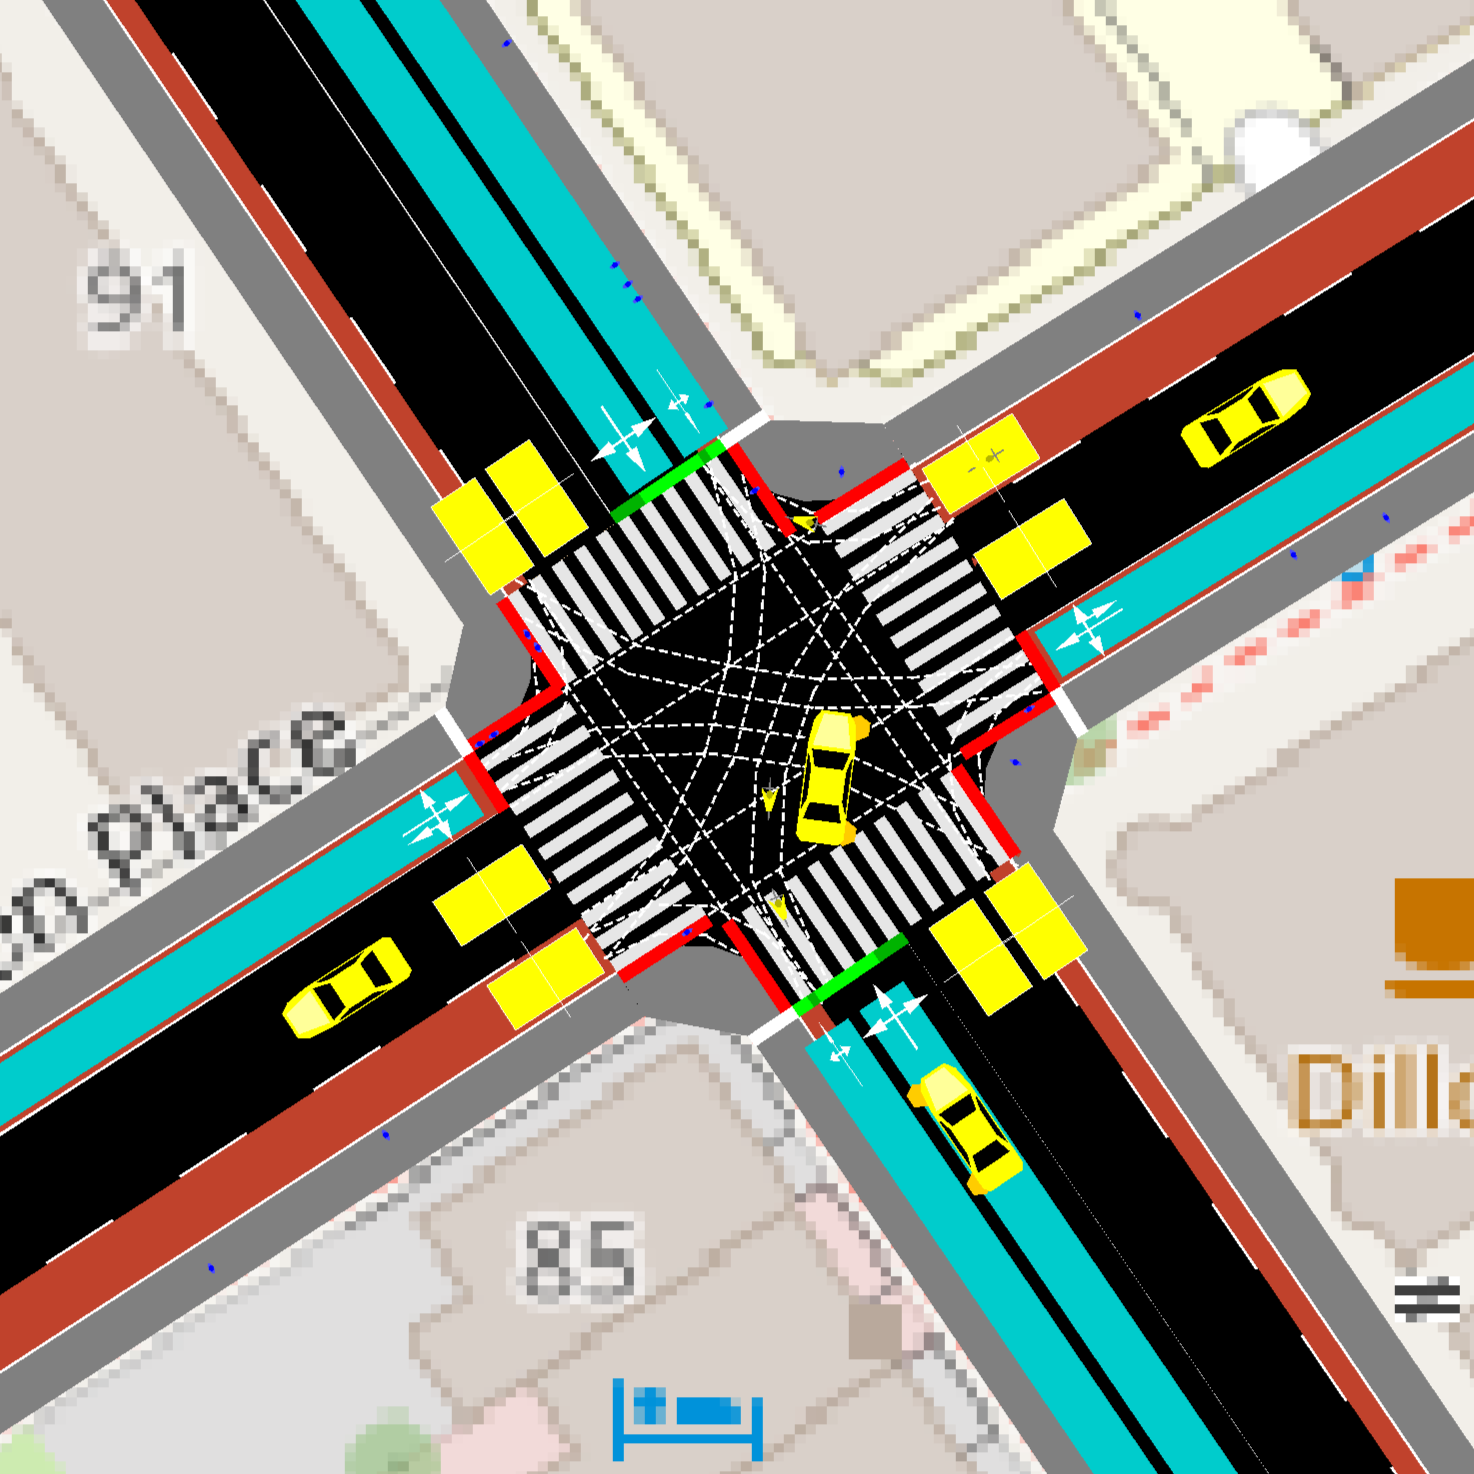
\includegraphics[width=\textwidth]{images/abstract_cover.png}
    \end{subfigure}
\end{figure}

\tableofcontents

\chapter{Introduction} \label{chapter:introduction}

\pagenumbering{arabic}
\setcounter{page}{1}

\section{The Problem}
Traffic lights are ubiquitous signalling devices used to control the flow of vehicle and pedestrian traffic, primarily for safety and better regulation of traffic. First introduced in 1868 on Parliament Square in London \cite{ThamesLeisureFacts2017}, there have been a wide range of designs created with the most common being a three-colour design -- that is green, amber, and red.

The three-colour de jure standard typically uses an internal clock to cycle through and control the duration of each signal phase in a pre-programmed pattern. Whilst this is an obvious approach, the fixed timer takes for granted that traffic demand will remain relatively constant over time, disregarding finer granularity and variations in conditions.

In an endeavour to improve upon this, advanced traffic light systems equipped with sensors are progressively being introduced. These systems dynamically adapt signal timings in response to observed traffic conditions by using rule-based logic and manually designed heuristics. This approach offers improvements in waiting times and vehicle throughput \cite{FHWA_ASCT17}, however it relies on predefined rules defined by domain experts that may fail to generalise and perform optimally in all conditions.

\section{Aim and Objectives}

The overall aim of this dissertation will be to perform a detailed analysis and evaluation of how an intelligent agent may be used to hopefully improve upon existing traffic light systems. Rather than explicitly defining behaviour in different traffic scenarios, we will observe how optimal decision-making policies may be learnt independently through the use of decentralised reinforcement learning algorithms.

Based on this aim, the following objectives are defined:

\begin{enumerate}
  \item Construct an environment in which our experiments will be conducted.
  \begin{enumerate}
    \item Define the boundaries of the environment.
    \item Research and understand available tools for traffic simulation.
    \item Build the abstracted computer representation.
  \end{enumerate}
  \item Develop our own intelligent agents in a progressive manner.
  \begin{enumerate}
    \item Review current traffic light systems in use.
    \item Explore the foundations of intelligent agents.
    \item Develop our reinforcement learning algorithms from first principles.
    \item Incrementally improve the algorithms with justifications.
  \end{enumerate}
  \item Evaluate the intelligent agents in the simulated environment.
  \begin{enumerate}
    \item Train and evaluate the agents in diverse scenarios.
    \item Consider the impact on both pedestrians and vehicles (i.e.\ via a reward system).
    \item Assess the feasibility of our agents and considerations in reality.
  \end{enumerate}
\end{enumerate}

Time is a currency that once spent cannot be regained. Traffic lights govern our lives to the extent that saving mere fractions of a second at the individual level can compound to an indescribable amount saved when considering the aggregate. By leveraging intelligent agents, this research hopes to take traffic lights a step further -- regardless of how big that step may be.

\section{Report Overview}

The main content of the report is structured as shown below, with the goal of each chapter flowing naturally from the previous, rather than in a way that is jarring. It should be noted that the objectives above are not necessarily reached in the report in the order they were defined in.

\begin{description}
    \item[Chapter \ref{chapter:introduction}] \textbf{-- Introduction} \\ This chapter. Gives an overview of the project.
    \item[Chapter \ref{chapter:literature_review}] \textbf{-- Literature Review} \\ Details the existing traffic systems: fixed-time control, vehicle-actuated control, and adaptive traffic control systems, and motivates our reinforcement learning algorithms. 
    \item[Chapter \ref{chapter:simulated_environment}] \textbf{-- Simulated Environment} \\ Defines the environment scope and describes the creation of the simulated environments including parameters for traffic generation.
    \item[Chapter \ref{chapter:reward_system}] \textbf{-- Reward System} \\ Explores the creation of a baseline environment from which we derive a reward formula (that accounts for pedestrians and vehicles) crucial for our agents.
    \item[Chapter \ref{chapter:q_learning}] \textbf{-- Q-Learning} \\ This chapter firstly explores the background of reinforcement learning, and then the Q-learning algorithm is implemented from scratch, before the limitations are discussed.
    \item[Chapter \ref{chapter:deep_q_learning}] \textbf{-- Deep Q-Learning} \\ Builds upon the Q-learning algorithm with the use of deep Q-networks, which we implement and evaluate the performance of in varying conditions.
    \item[Chapter \ref{chapter:communicative_deep_q_learning}] \textbf{-- Communicative Deep Q-Learning} \\ Takes the previous algorithms even further with the introduction of a network layer and communication bus, which we implement before the inherent limitations are discussed.
    \item[Chapter \ref{chapter:conclusions}] \textbf{-- Conclusions} \\ We conclude with an evaluation of our intelligent agents equipped with decentralised reinforcement learning, and consider what extensions could be made in the \emph{future}.
\end{description}

\chapter{Literature Review} \label{chapter:literature_review}

Modern traffic light control has changed significantly over the years, ranging from simple fixed-time mechanisms to complex adaptive and coordinated systems. Broadly speaking, systems can be categorised into three main types: fixed-time control, vehicle-actuated control, or adaptive traffic control. These will explored in this chapter, as well as the motivations for introducing intelligent agents.

\section{Fixed-Time Control}

Fixed-time traffic signals operate according to a predetermined schedule. Signal phases and cycle lengths are configured in advanced, typically using historical data \cite{GoelBusGershenson}. The controller cycles repeatedly through these phases regardless of traffic conditions.

Such systems are predictable and inexpensive, used in city centers, interchanges, or roadworks. However, they assume stable traffic patterns. During periods of unusual demand, fixed-time systems cannot respond dynamically, leading to inefficient utilisation of junctions.

\section{Vehicle-Actuated Control}

Actuated systems are an improvement over purely fixed-time control systems. These systems utilise sensors -- such as inductive loop detectors or cameras -- to detect vehicles. Pedestrians can also use push buttons to register their presence \cite{PedestrianCrossings23}. This may for example enable one route at an intersection to stay active if other routes are barren.

Typically used in rural roads or highway operations, they may be semi-actuated, where detectors are only placed on side approaches, or fully actuated, in which detectors are installed on all approaches. Overall, responsiveness to traffic conditions is improved, reducing unnecessary waiting. However, it relies on rule-based logic and manually defined heuristics, which may fail to perform optimally in all conditions \cite{LiPengHouEtAl2023}.

\section{Adaptive Traffic Control}

Unlike fixed-time or purely vehicle-actuated control systems, adaptive traffic control enables signal timings to be adjusted in real time based on observed traffic conditions. Data is collected from inductive loops, cameras, or other technologies.

By modifying parameters such as cycle length, phase splits, and offsets in response to traffic \cite{LiPengHouEtAl2023}, adaptive controllers seek to reduce delays, smooth traffic flow, and increase throughput (though it may also be used to \emph{discourage} high volumes of traffic at the request of local residents for example).

Split Cycle Offset Optimisation Technique (SCOOT) and the Sydney Coordinated Adaptive Traffic System (SCATS) are two examples widely deployed in urban areas. These systems group signals into regions and make dynamic adjustments to balance delays and improve coordination. This helps promote ``green waves'', where vehicles encounter consecutive green lights without having to stop, but possibly with added pedestrian and cyclist delays \cite{CesmeUrbanikII2021}.

SCOOT has demonstrated an improvement in traffic performance of order of 15\% compared to fixed-time control systems \cite{ITS2012}. In London, with the introduction of the cloud-based Real Time Optimiser platform, this is being replaced with FUSION -- intended to bring even further improvements. However, these systems still rely on human-designed algorithms. Optimal strategies are not necessarily ``learnt'', nor does it adapt to every possible traffic scenario without explicit modeling by engineers.

\section{Limitations}

Existing traffic light systems work well enough, however there are several fundamental limitations.

Firstly, these systems rely on parameter tuning and predefined logic. Even for adaptive traffic control the optimisation strategies used are engineered by domain experts. Performance is constrained by assumptions embedded in the design and, when traffic conditions deviate from these, optimality is not guaranteed.

Secondly, most traditional systems are designed such that they prioritise vehicular throughput. Pedestrians and cyclists are typically the secondary optimisation target. This may lead to scenarios in which vehicles reap the benefits at the expense of pedestrians who may see increased waiting times.

Thirdly, these systems are limited with regards to learning. Although adaptive traffic control systems respond in real time, they do not learn from historical experience in the sense of improving their strategy. Parameters may be recalibrated periodically by engineers, but this is not autonomous and novel strategies may be missed. Considering the scale of these systems, it may be hard to consider all possible variables.

Finally, implementation and maintenance costs are non-trivial. These systems require extensive sensor and communication infrastructure, calibration, as well as continuous monitoring by traffic engineers. The complexity of these systems also make them less transparent and harder to validate formally with respect to performance benefits.

\section{Motivation for Reinforcement Learning}

Reinforcement learning offers an alternative method of traffic signal control. Control policies are not explicitly programmed, but instead emerge through intelligent agents interacting with a traffic environment. An intelligent agent can observe current traffic state, select a signal phase action, and receive feedback in the form of a reward from the environment.

Over time, behaviour gradually improves and a control strategy emerges through experience, as opposed to encoding behaviour manually for every possible scenario. The ability to learn makes this very powerful; most limitations discovered above are mitigated by learning -- though perhaps not the infrastructure costs. Ergo, this will be explored for the remainder of this dissertation.

\section{Existing Reinforcement Learning Implementations}

A comprehensive set of publications and resources relating to reinforcement learning for traffic light control was kindly collated by the Intelligent Transportation Systems Society (ITSS) of Pennsylvania State University \cite{ITSS2020}. There were a breadth of reinforcement learning algorithms explored to solve the problem of optimising traffic light signals.

The core idea common amongst the publications was to implement a centralised controller which has access to all traffic light systems in an environment, as opposed to each traffic light system being independently controlled by decentralised agents. This will be the key point which will differentiate our agents.

We will cover the implementation of reinforcement learning algorithms from first principles, and incrementally justify and build to more complex algorithms. Existing publications tend to curvet over the foundations and use powerful pre-existing libraries. Whilst they serve as excellent resources, we will not be referring to these; our environment and agents will be built orthogonally from the ground up.

\section{Summary}

This chapter described the fixed-time control, vehicle-actuated control, and adaptive traffic control systems in detail, mentioning the benefits and drawbacks of each. The fundamental limitations of these systems as a whole were also explored, motivating why a novel approach which uses reinforcement learning is desirable.

\chapter{Simulated Environment} \label{chapter:simulated_environment}

% The main chapters should start with a brief summary -- this chapter is about, or introduces, some aspect of the work.
Before we get to our intelligent agents, we must first construct an environment where the agent can receive input -- or state, rather -- and perform actions. For the sake of simplicity this environment will be constrained to the streets surrounding University College London's (UCL) Bloomsbury Campus. This area provides scope sufficient for the agents to train well and generalise to other situations.

\section{OpenStreetMap}
OpenStreetMap is a map database maintained by a community of volunteers. Using their data obtained from ariel photo imagery, satellite imagery, geodata sources, as well as manual community additions \cite{HaklayWeberOSM08}, we can extract a portion of UCL's Bloomsbury Campus\footnotemark\footnotetext{The map centre is: 51.52519°N, 0.12870°W (WGS84).}, also complete with data such as traffic lights and crossings.

\begin{figure}[H]
    \centering
    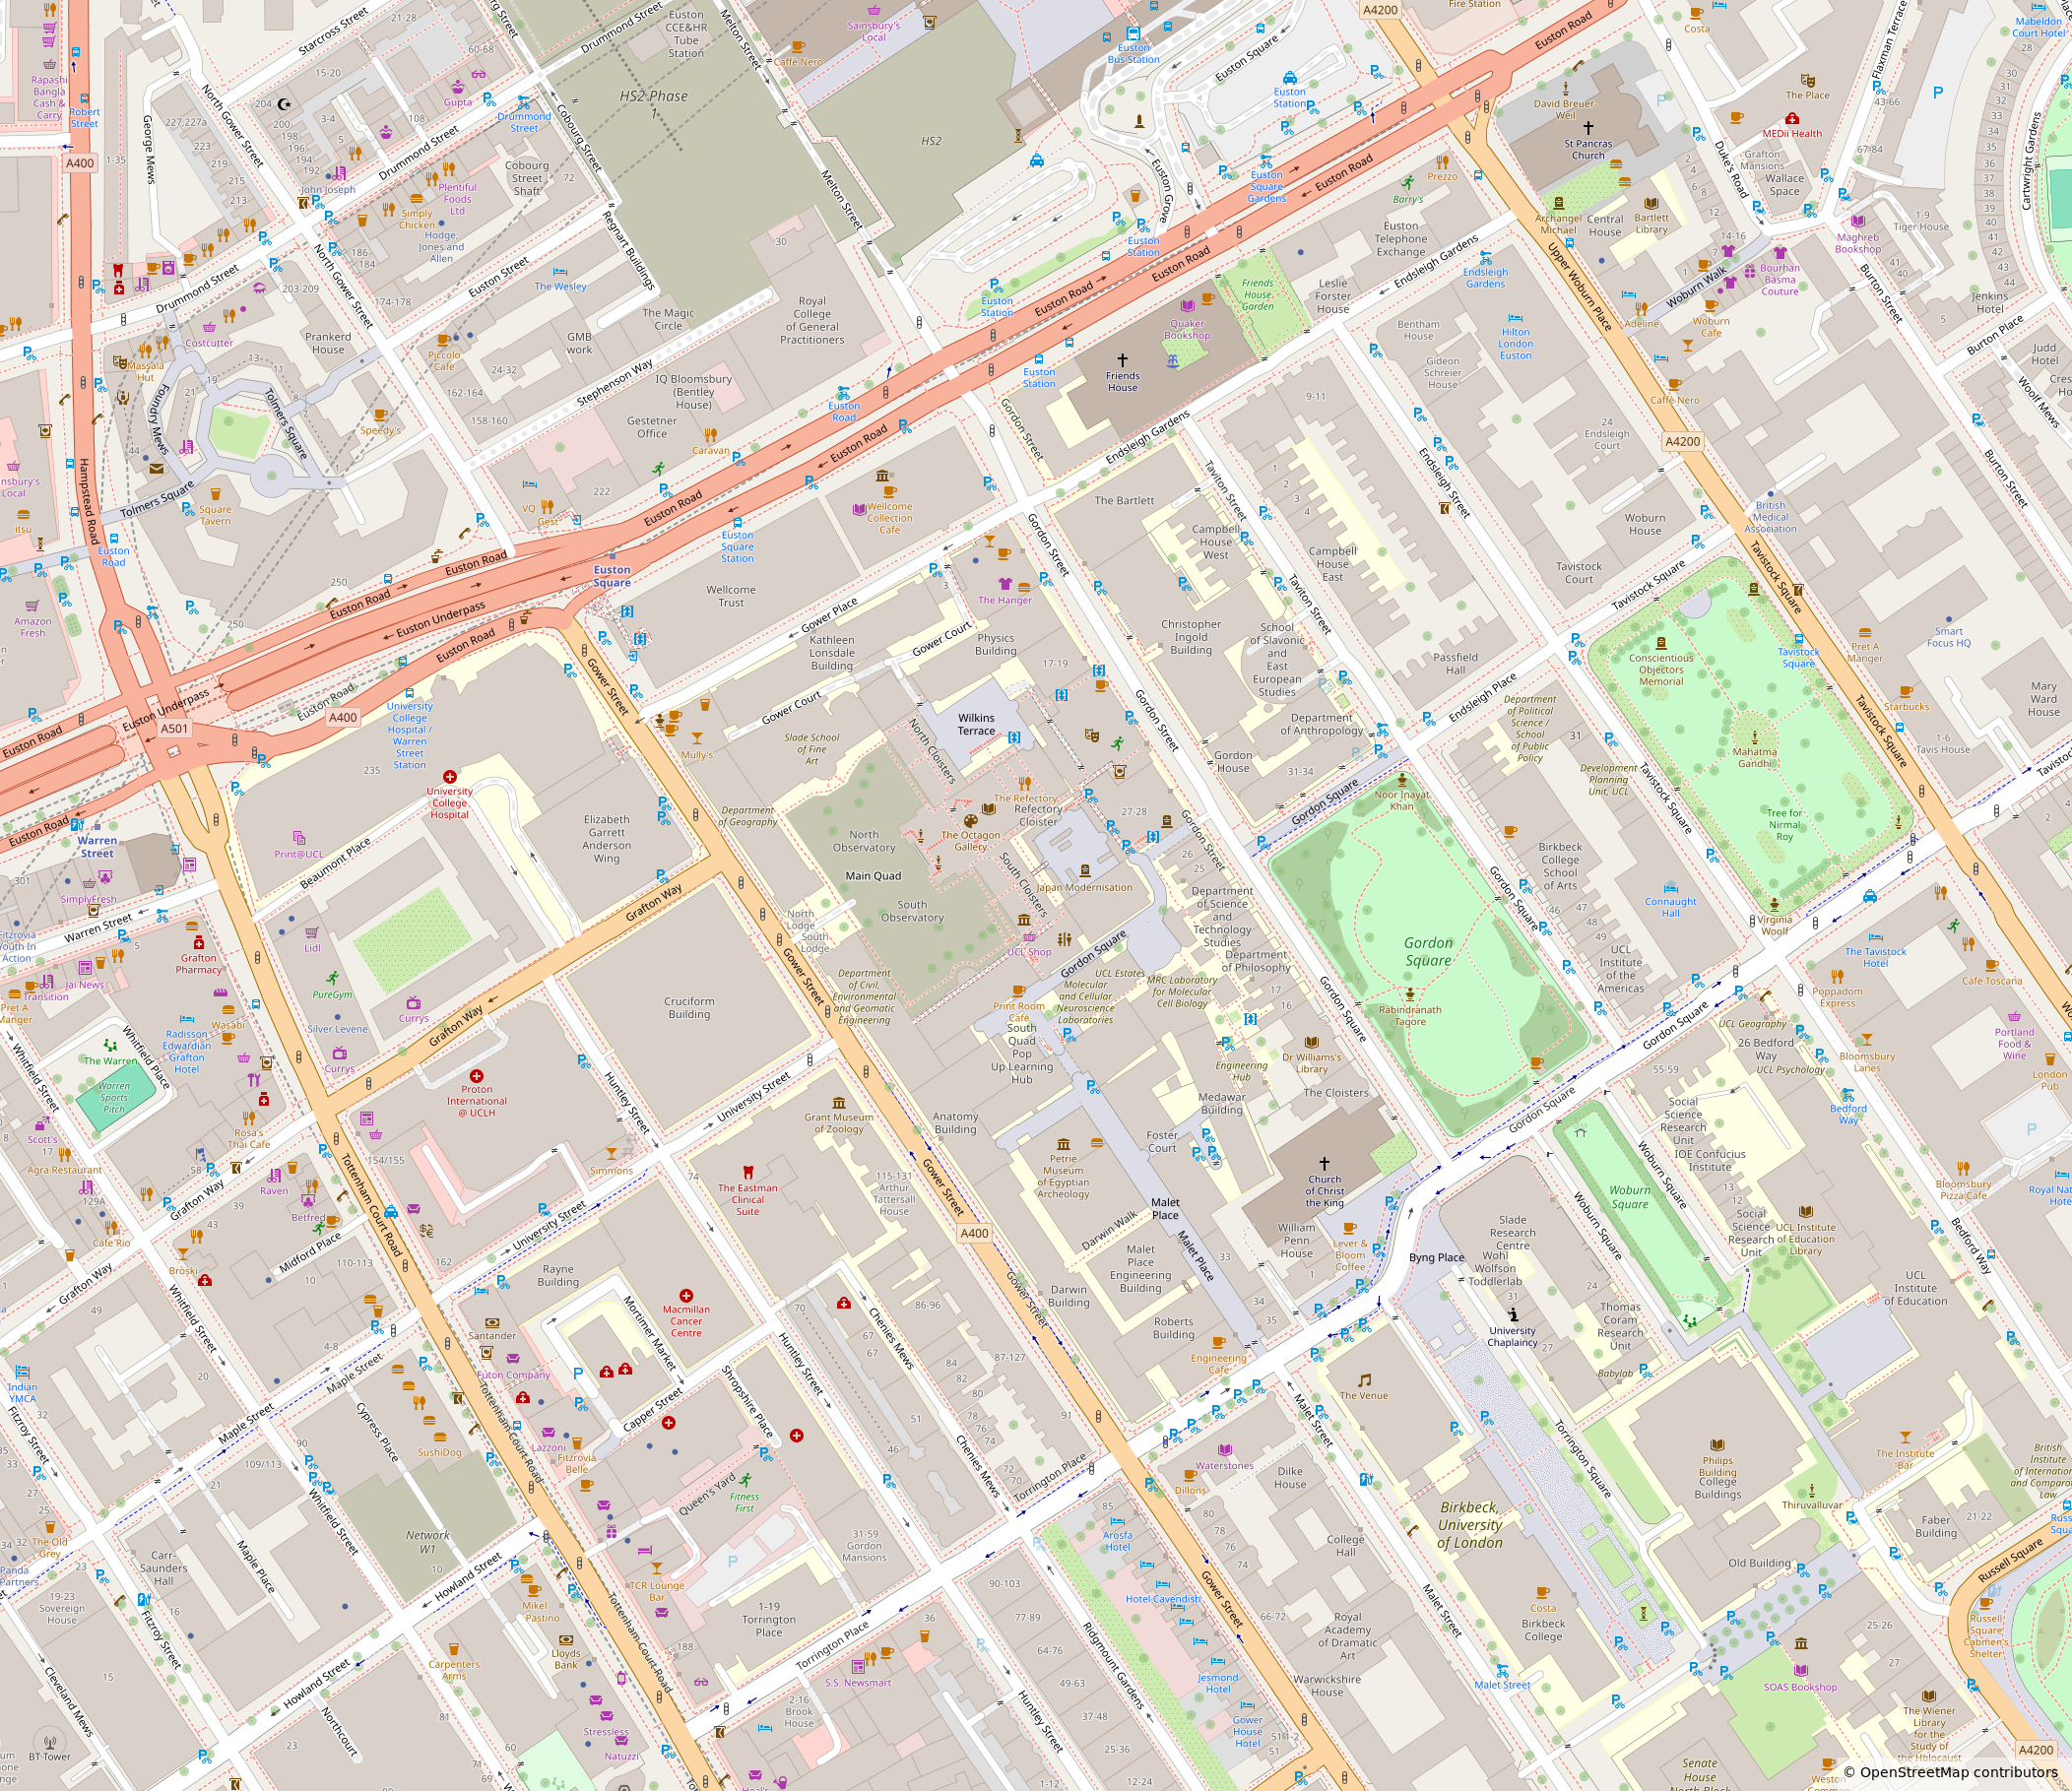
\includegraphics[width=0.70\textwidth]{images/ucl_bloomsbury_campus.png}
    \caption{Map of UCL's Bloomsbury Campus extracted from OpenStreetMap data.}
    \label{fig:ucl_bloomsbury_campus}
\end{figure}

Although the data from OpenStreetMap provides a lot of useful information, we will supplement it with Google Street View -- featured in the Google Maps software -- which provides interactive panoramas from positions along the streets. This will allows us to find out more precise information such as lane markings and widths.

\section{Simulation of Urban MObility}
Simulation of Urban MObility (SUMO) is an open source, multi-modal traffic simulation package designed to handle large networks. It allows for intermodal simulation including pedestrians and comes with a large set of tools for scenario creation.

Using the image in Figure~\ref{fig:ucl_bloomsbury_campus}, we can create a network using the \emph{netedit} graphical network editor included in SUMO. Networks are primarily comprised of edges, which is subdivided into lanes, and junctions, which are nodes where the edges meet. Junctions additionally support crossings, lane connections, and traffic lights.  

\begin{figure}[H]
    \centering
    \begin{subfigure}{0.48\textwidth}
        \centering
        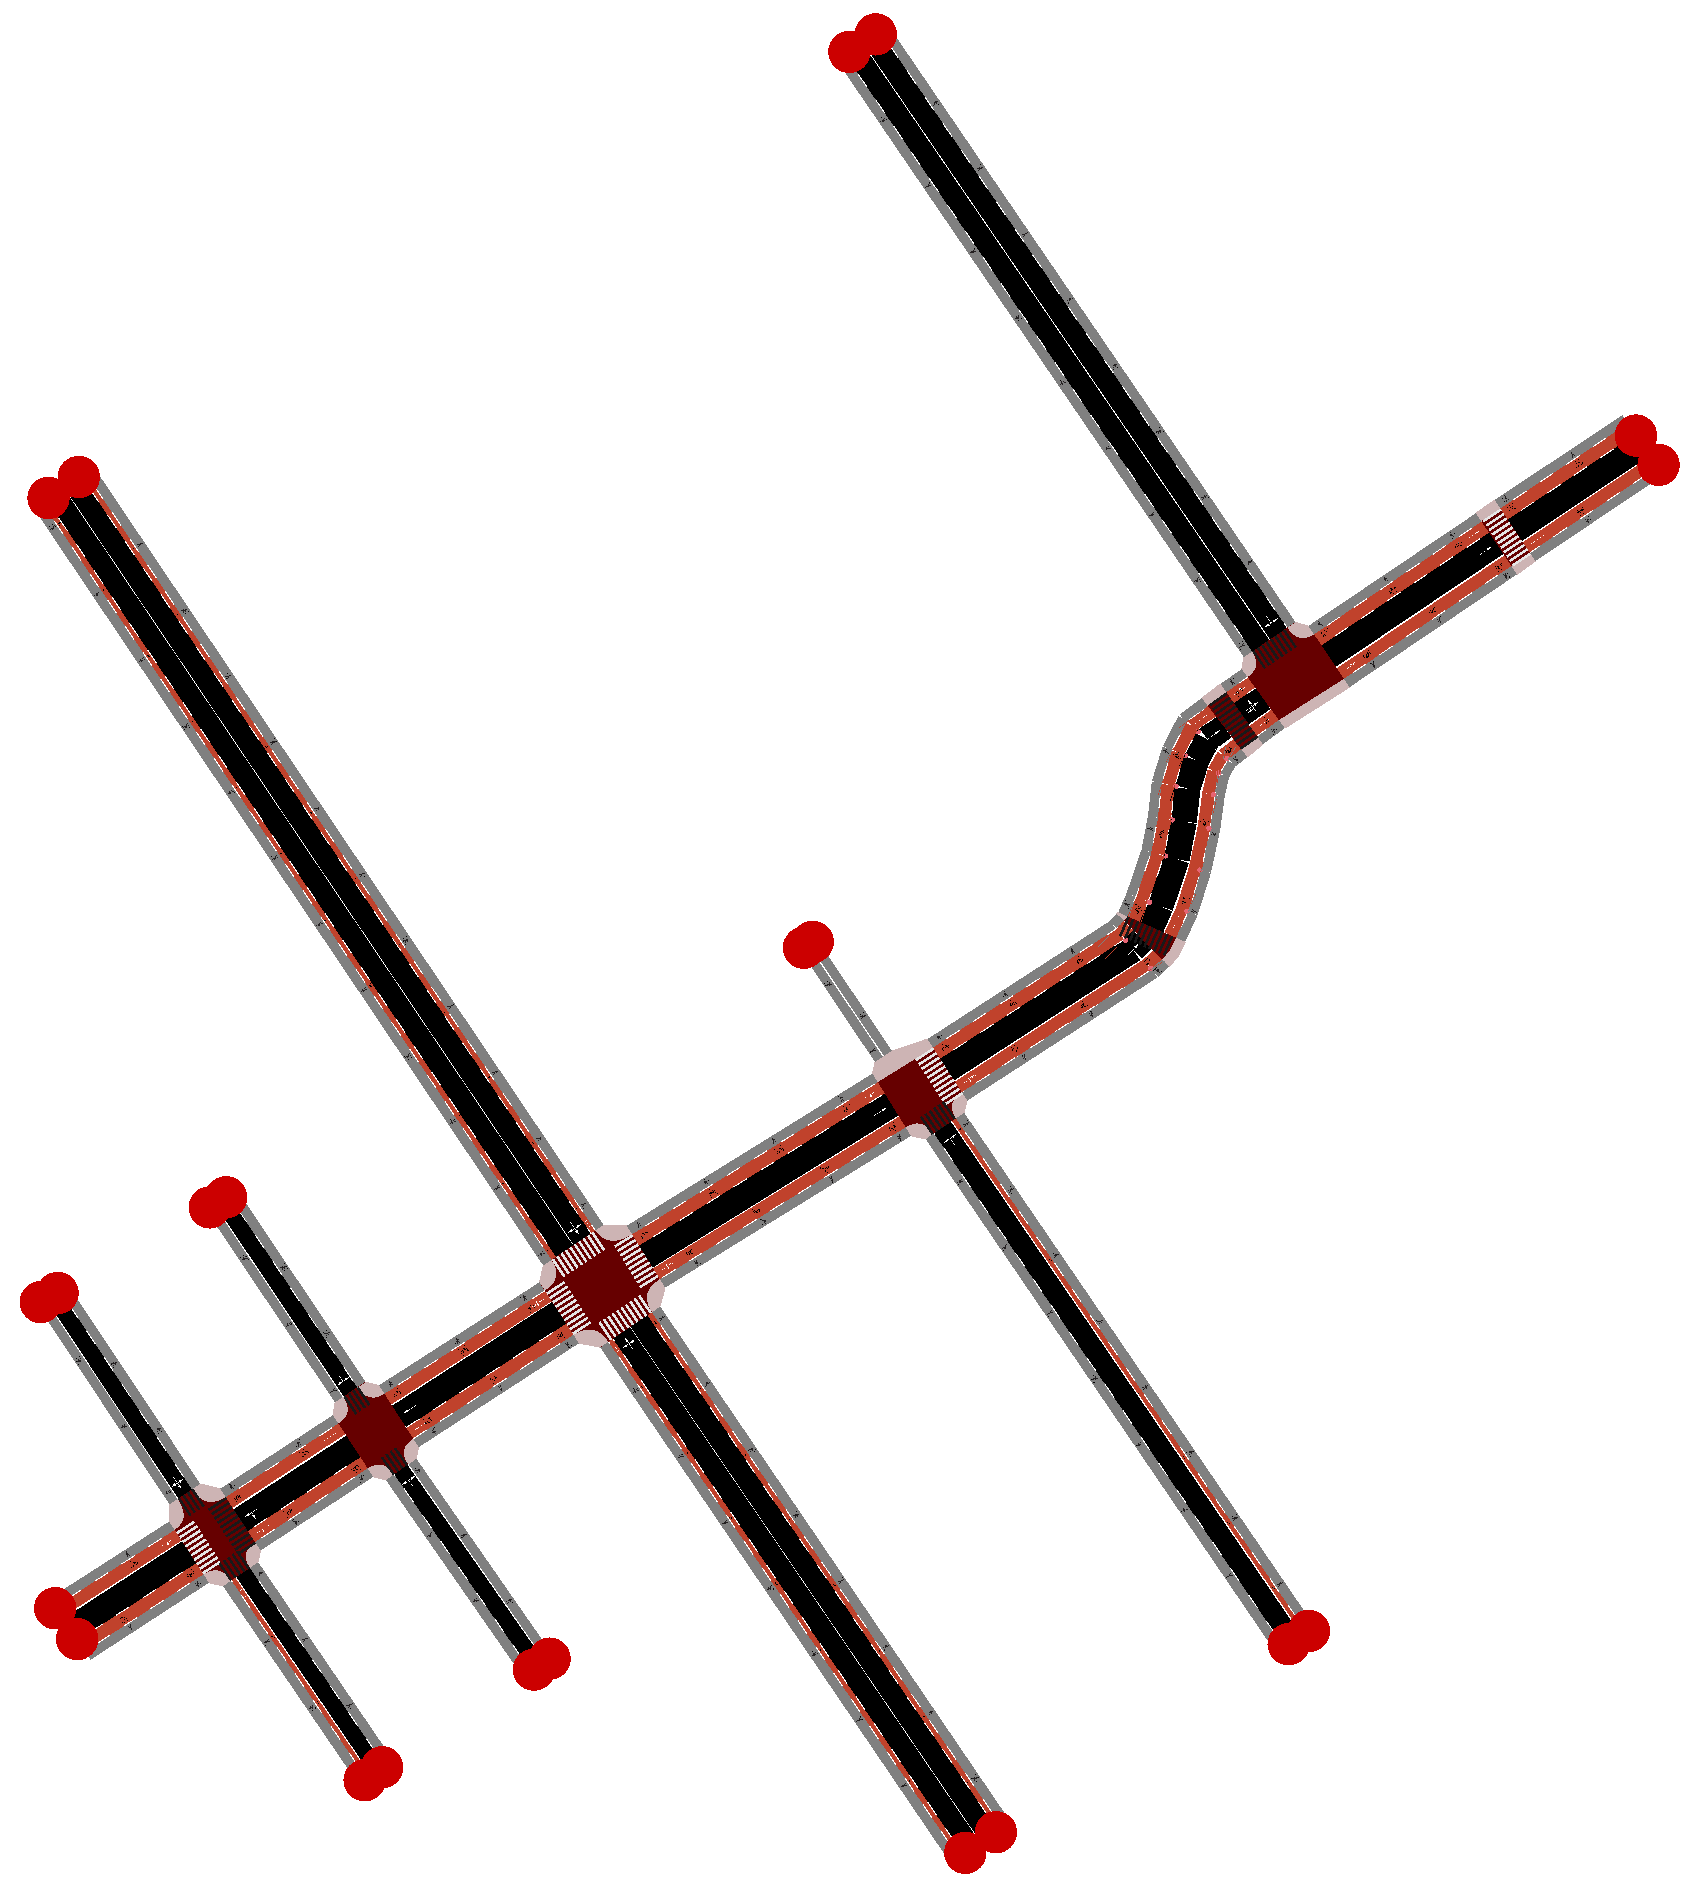
\includegraphics[width=\textwidth]{images/netedit_demo.png}
        \caption{Road network in netedit.}
        \label{fig:netedit_demo}
    \end{subfigure}
    \hfill
    \begin{subfigure}{0.48\textwidth}
        \centering
        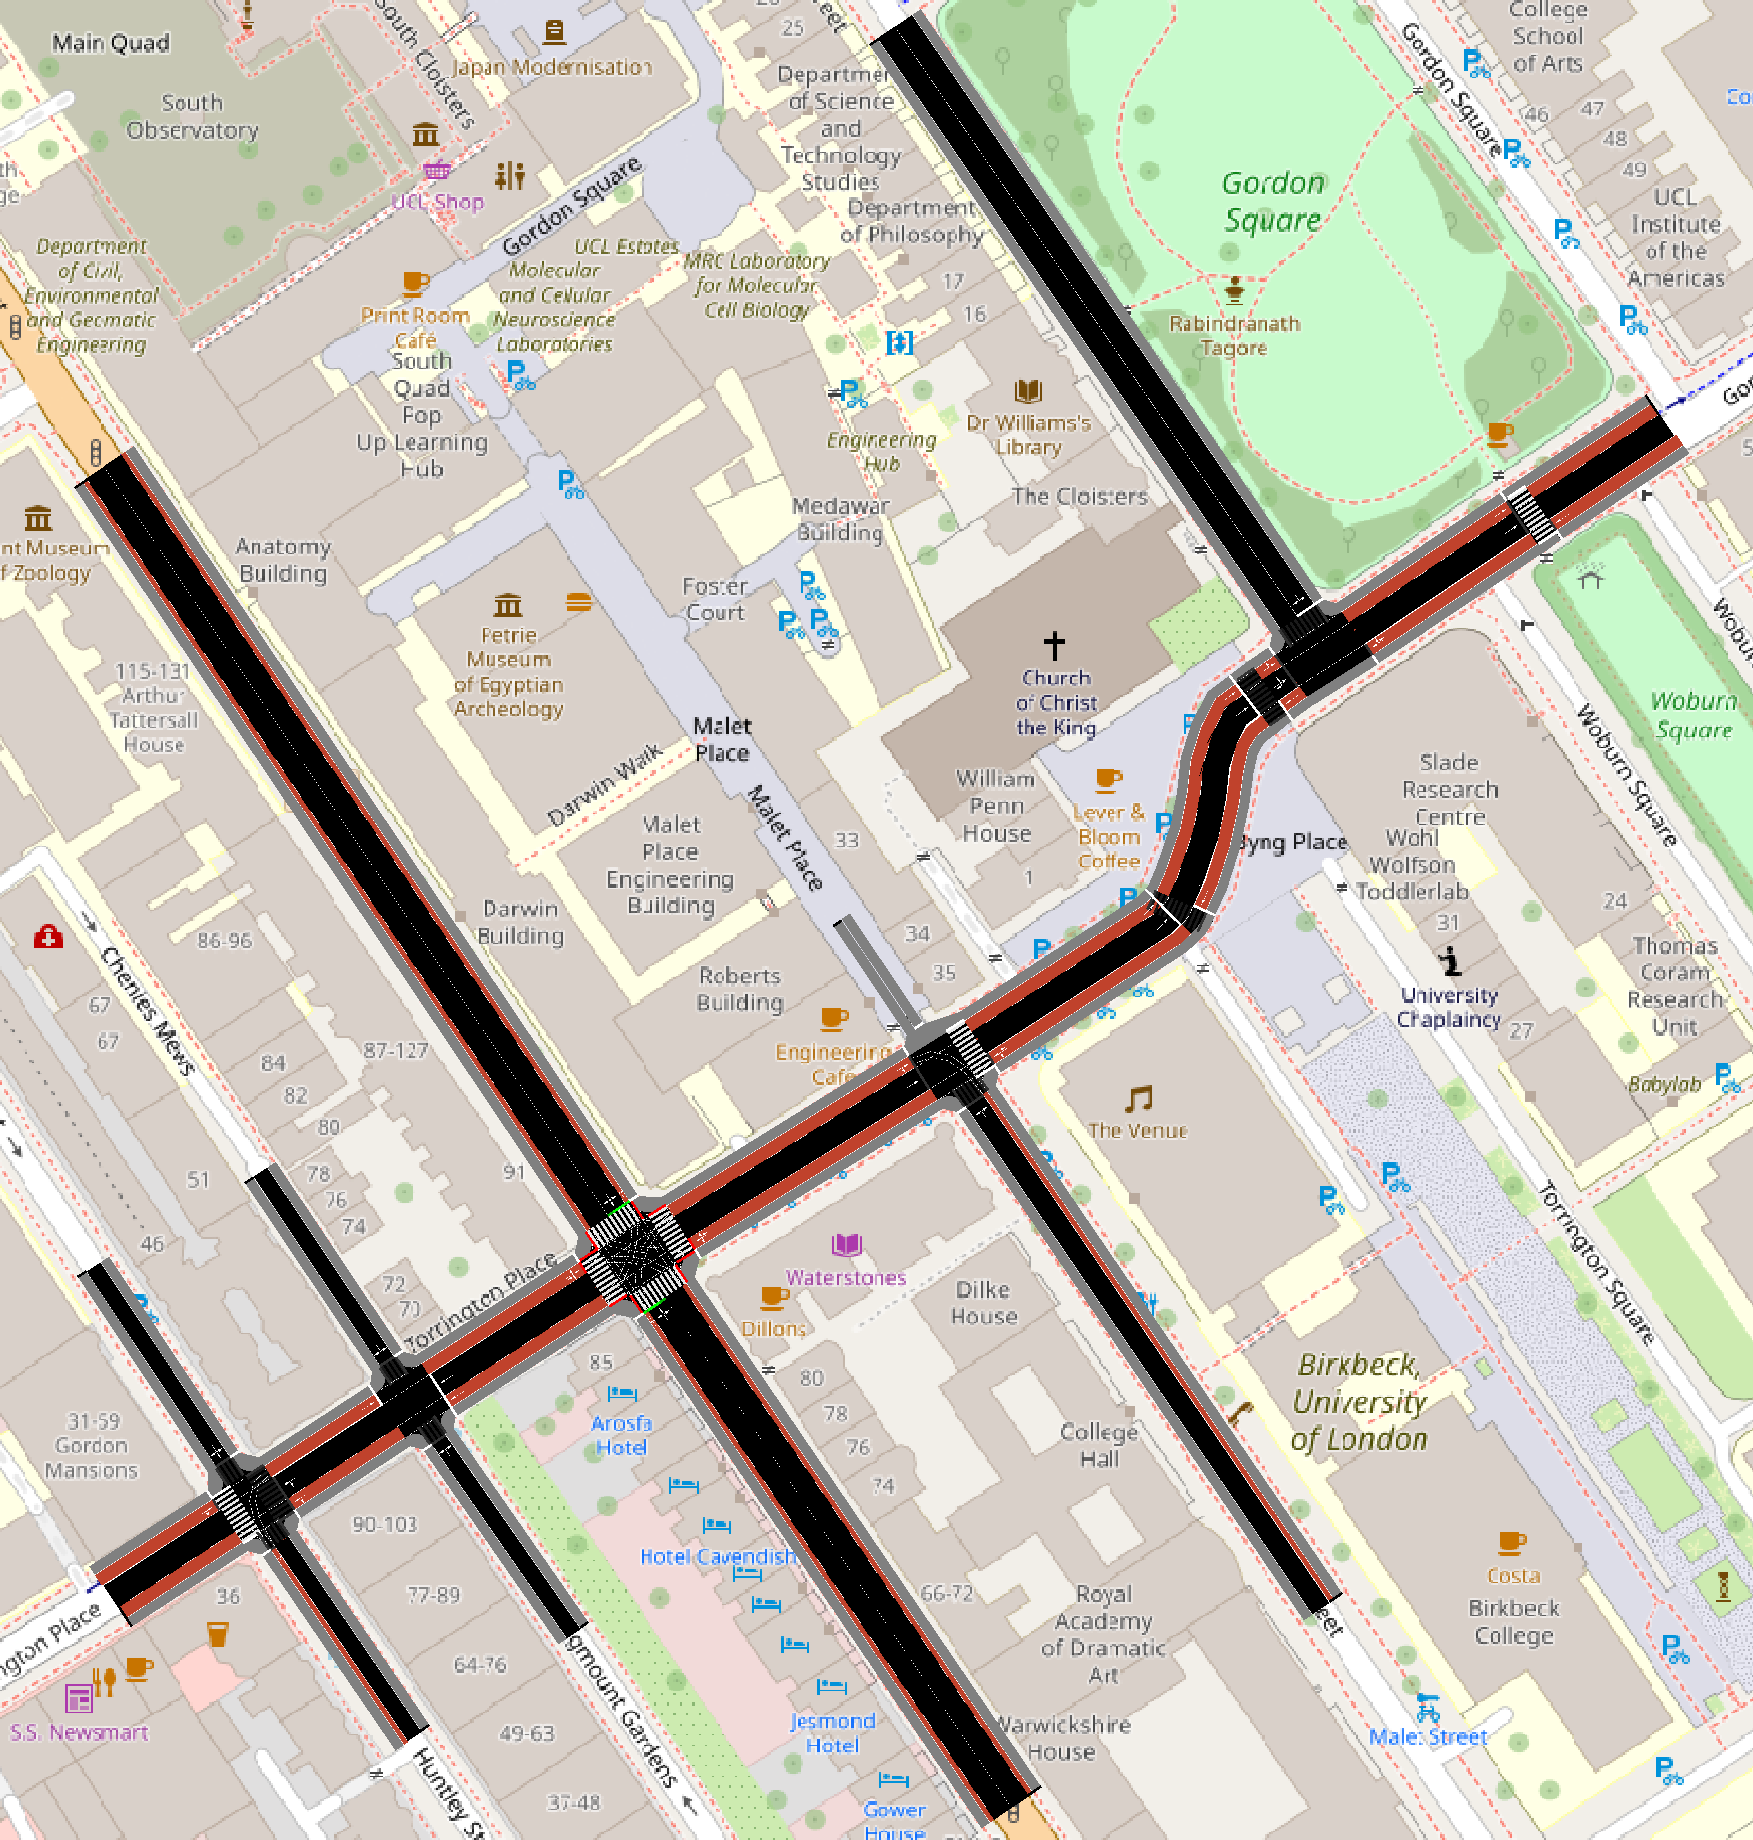
\includegraphics[width=\textwidth]{images/sumo_demo.png}
        \caption{Simulation view in SUMO.}
        \label{fig:sumo_demo}
    \end{subfigure}
    \caption{Demo simulation environment.}
    \label{fig:demo_simulation}
\end{figure}

In Figure~\ref{fig:netedit_demo}, the red circles and intermediary maroon links indicate junctions, whereas the in between sections are the edges. Each edge can be comprised of a bicycle lane, pedestrian lane, and/or vehicle lane as shown. Additionally, crossings have been added to the junctions, and a configurable traffic light system has been added with the lane connections appropriately adjusted.

Though not visible in the road geometry, lane and junction priorities have also been set, consistent with rules 170--183 of The Highway Code \cite{HighwayCode159to203}. In the UK, `main' and `side' roads are relative terms, with the road with priority (e.g. no give-way markings, or priority road signs) functioning as the main road, while the road required to give way is the side road.

Importantly, subtle issues such as bicycle lanes overlapping in such a way that `deadlocks' occasionally occurred in which bicycles indefinitely wait on the other to move, or pedestrians being `jammed' on narrow pavements due to there not being enough space were carefully resolved through manual editing. Figure~\ref{fig:demo_before_fix} gives an example of gridlocked entities.

\begin{figure}[H]
    \centering
    \begin{subfigure}{0.48\textwidth}
        \centering
        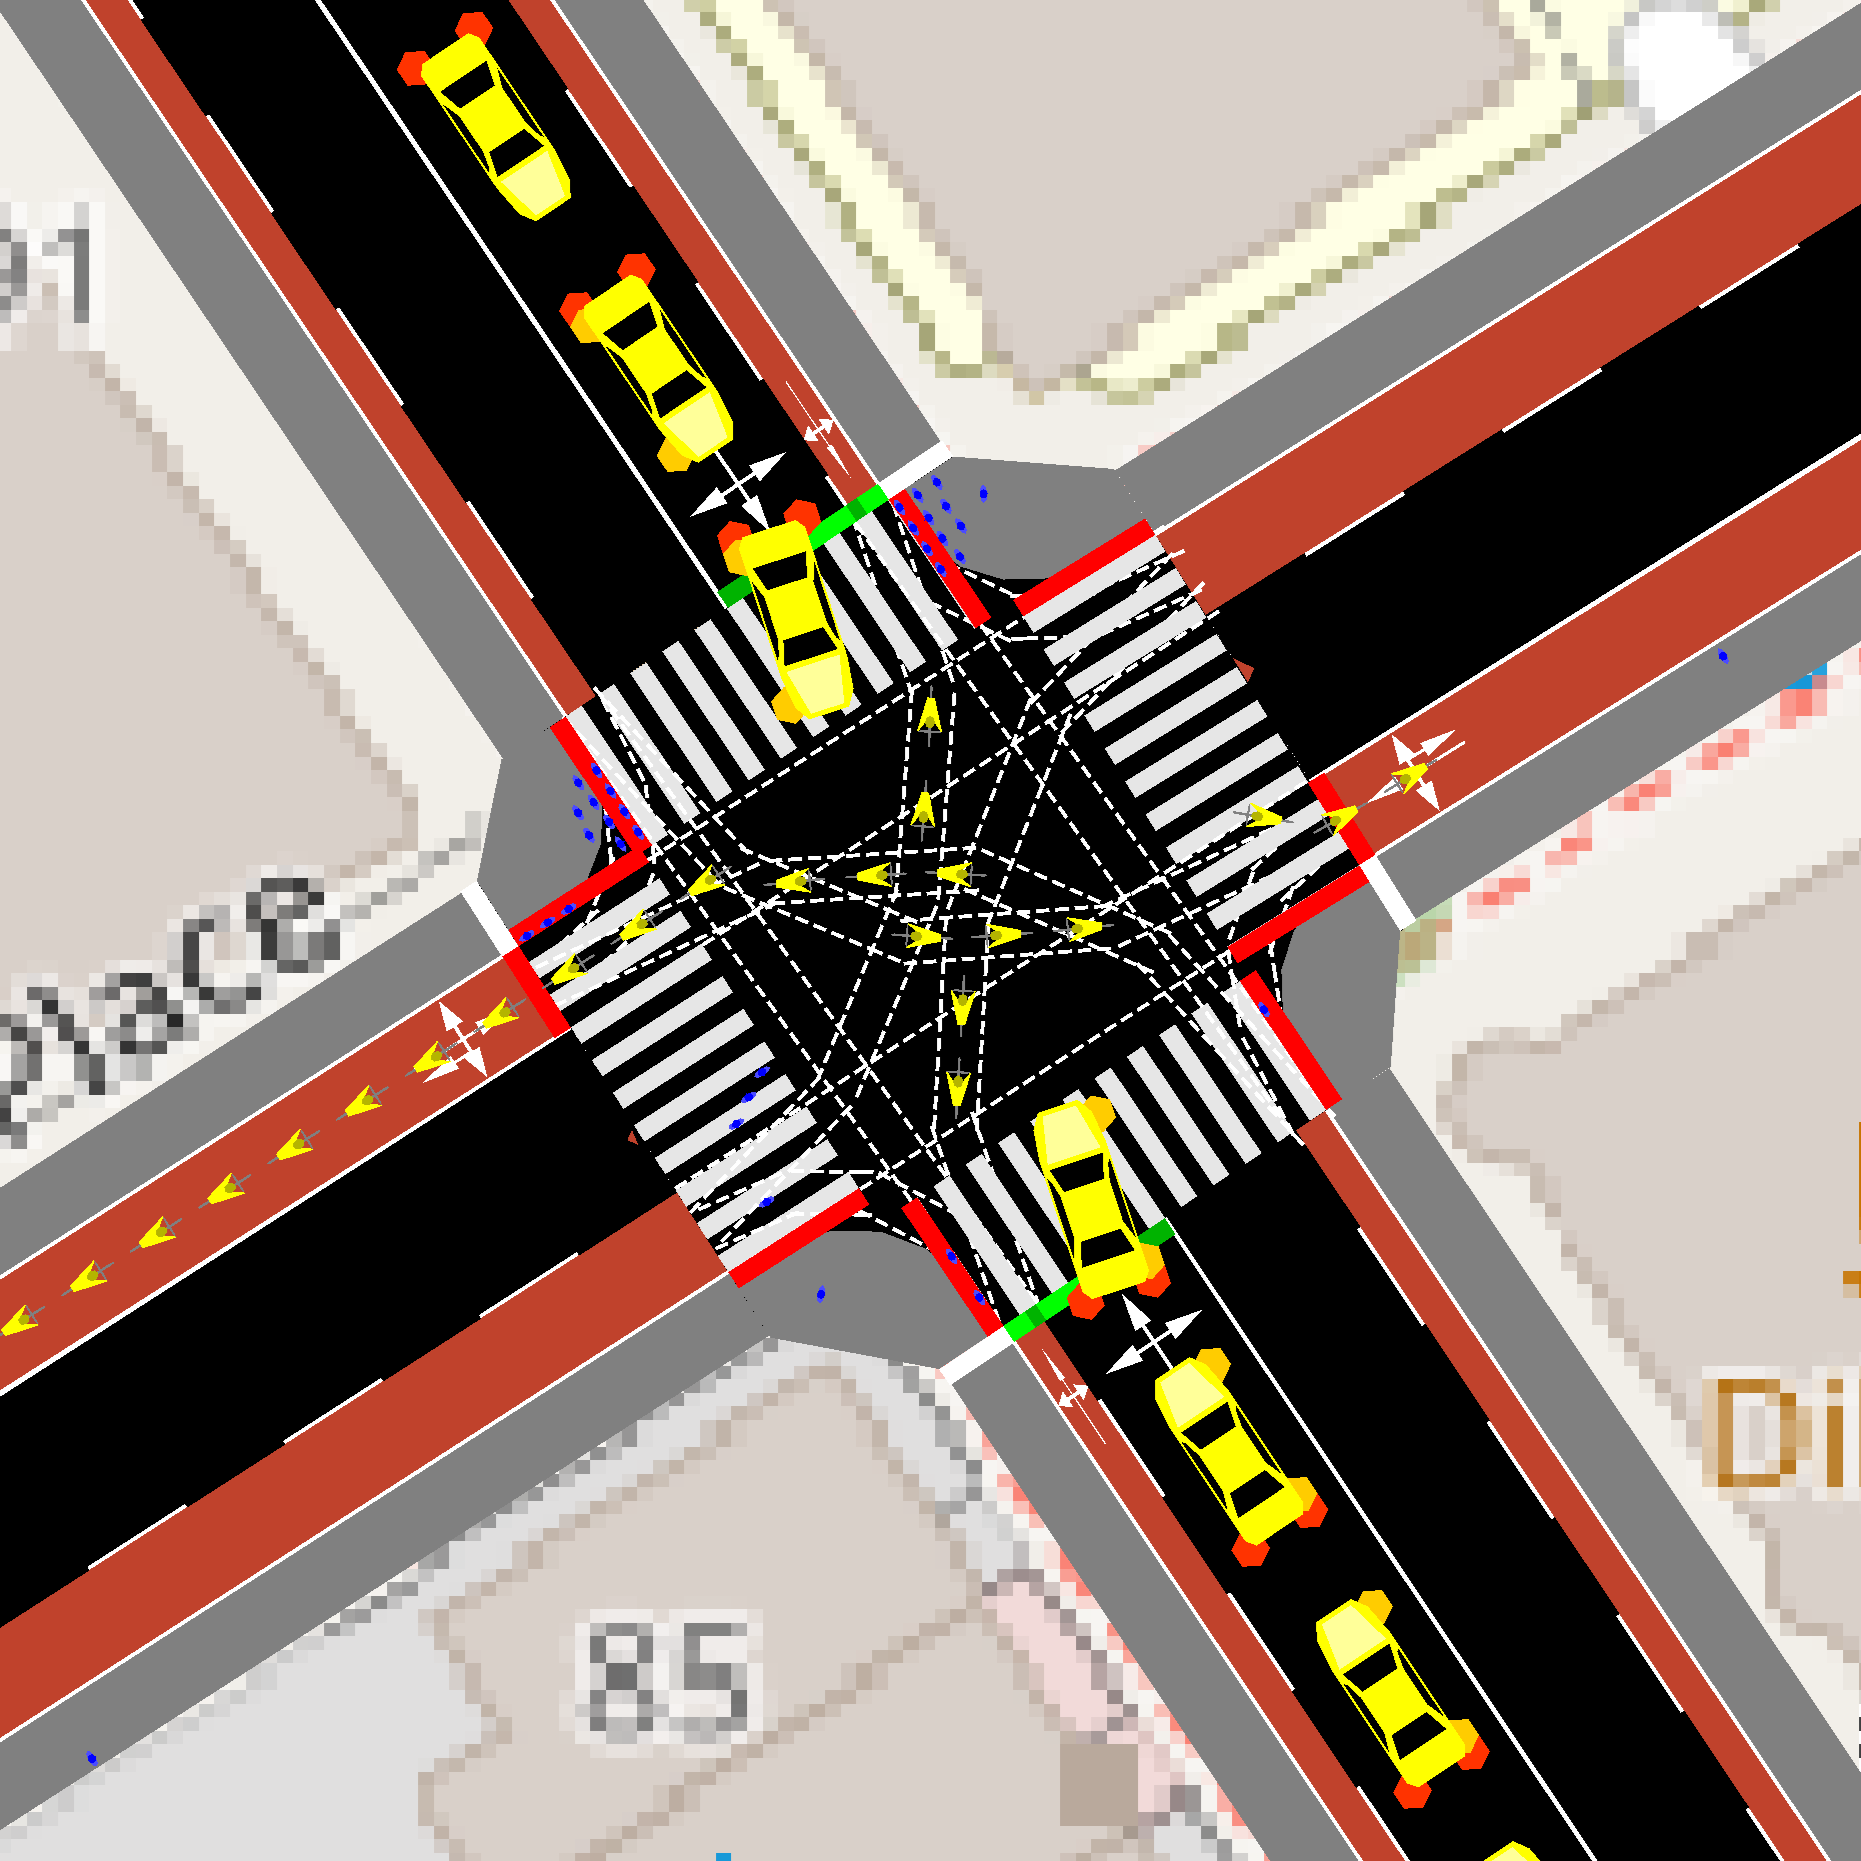
\includegraphics[width=\textwidth]{images/before_fix_demo.png}
        \caption{Before manual lane fixing.}
        \label{fig:demo_before_fix}
    \end{subfigure}
    \hfill
    \begin{subfigure}{0.48\textwidth}
        \centering
        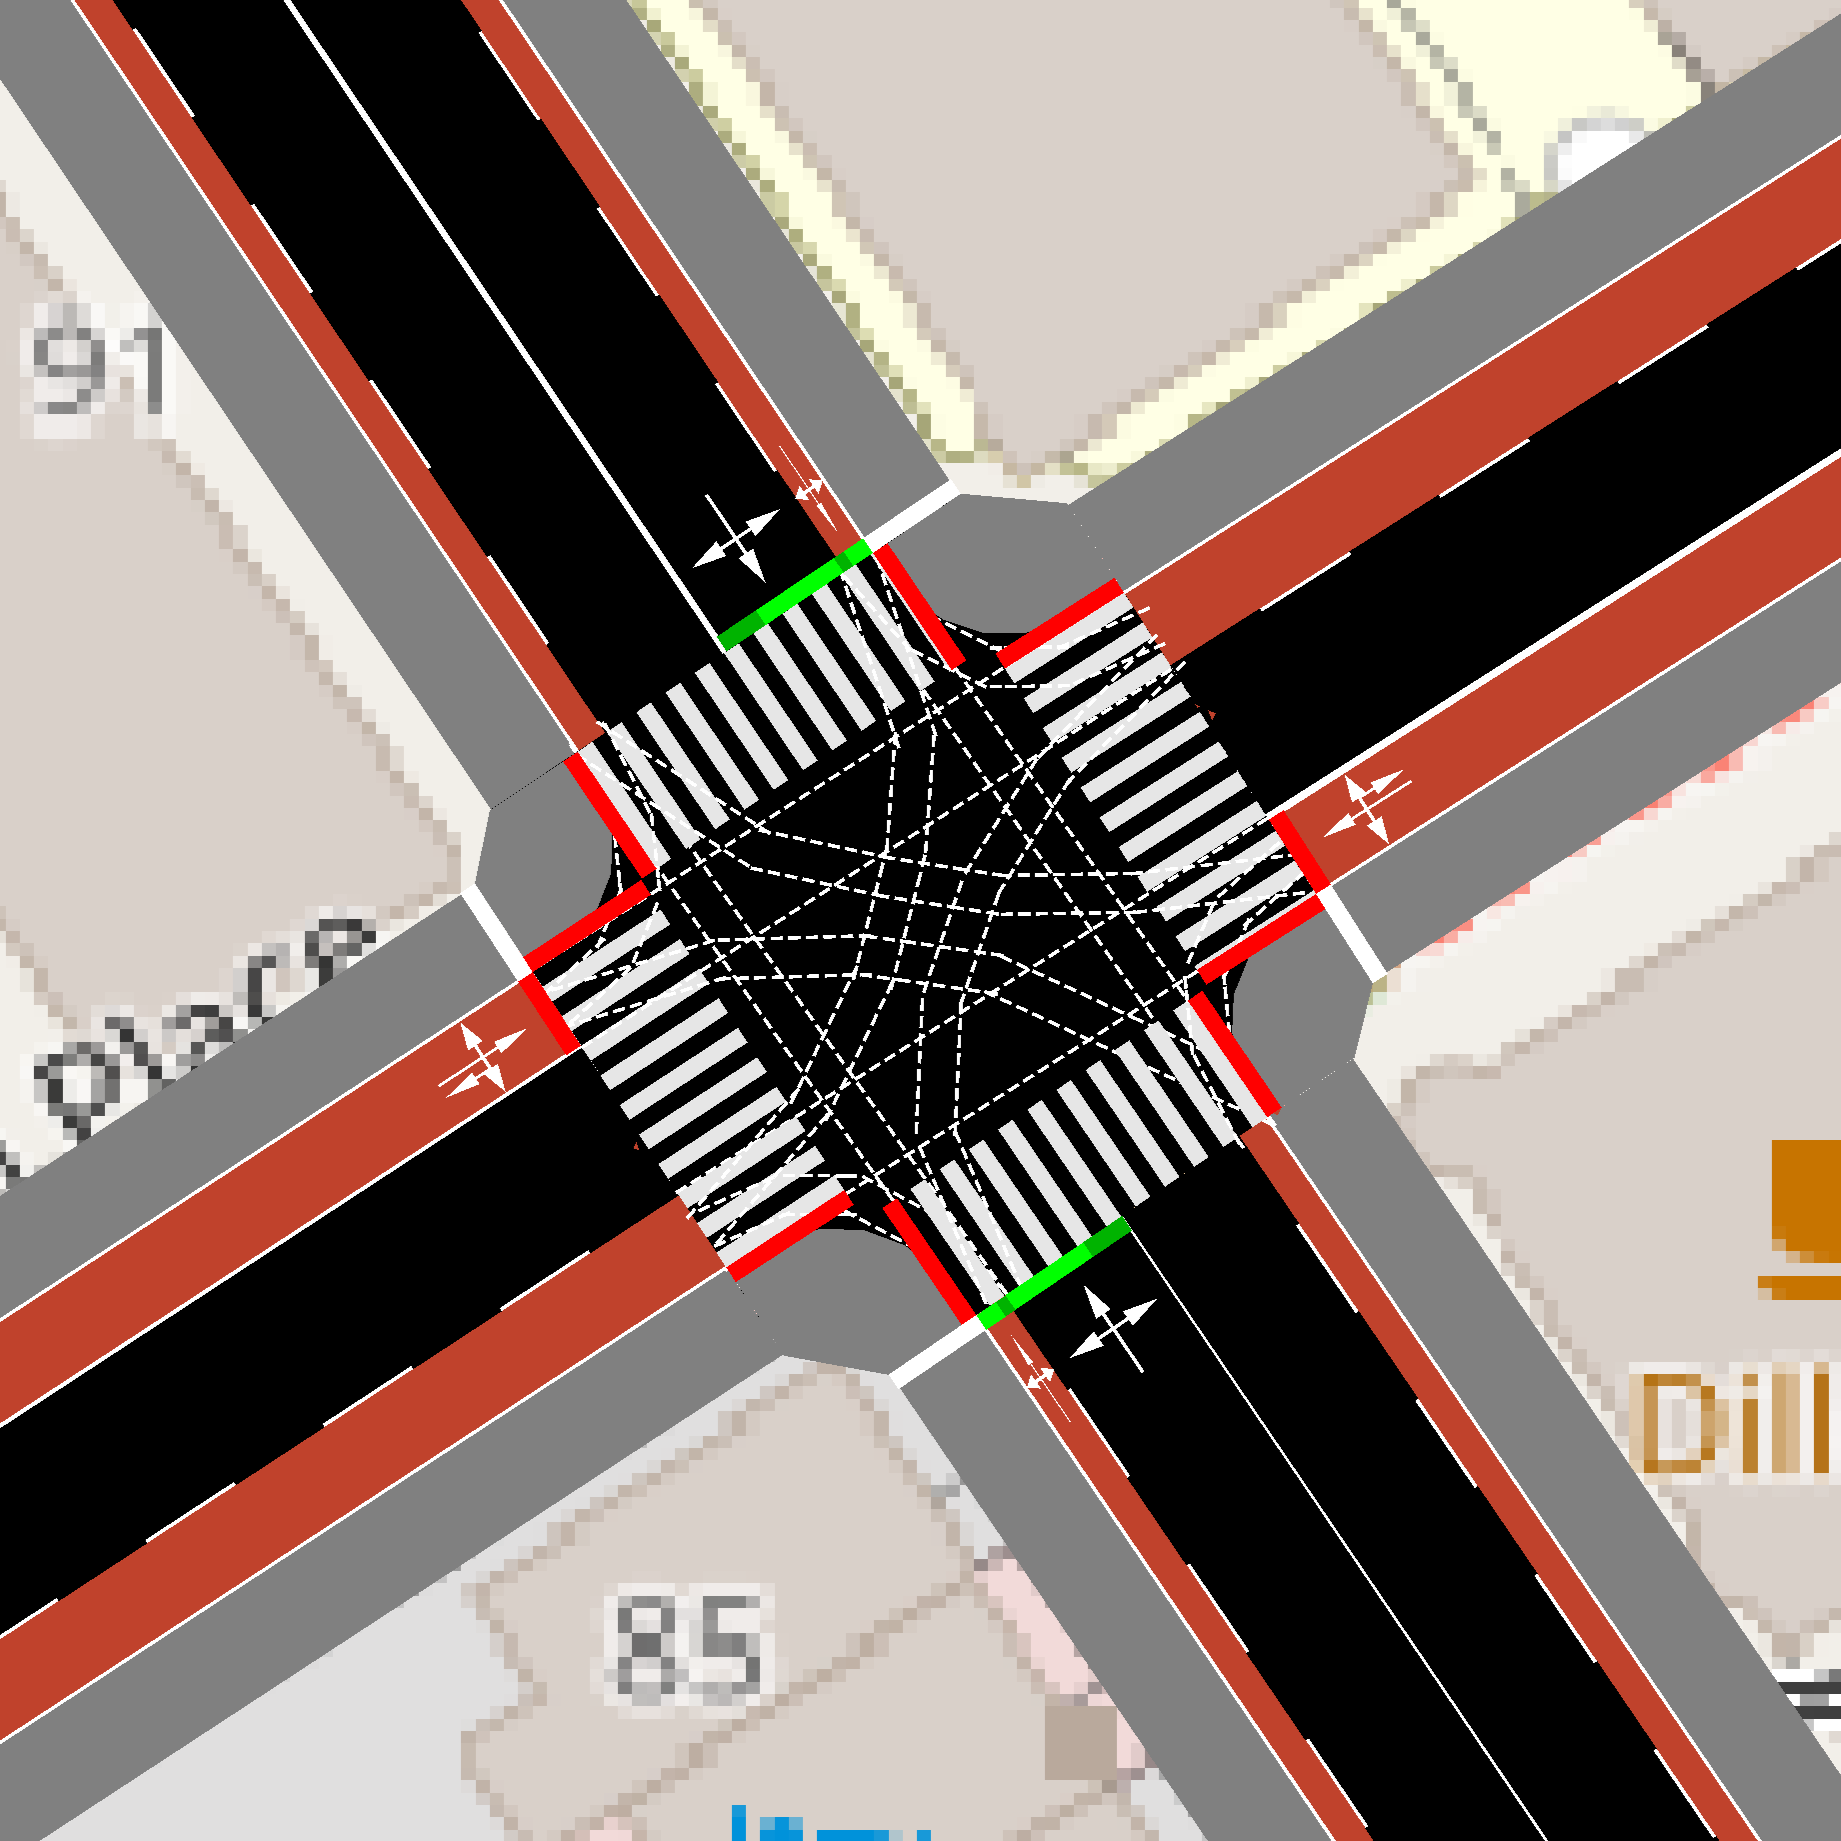
\includegraphics[width=\textwidth]{images/after_fix_demo.png}
        \caption{After manual lane fixing.}
        \label{fig:demo_after_fix}
    \end{subfigure}
    \caption{Demo network fix example of junction bicycle lanes.}
    \label{fig:demo_network_fix}
\end{figure}

\section{Route Generation}

The SUMO installation includes an additional collection of tools for convenience. One such tool is a \texttt{randomTrips.py} script written in Python which enables automatic generation of trips and routes\footnotemark\footnotetext{N.B. a \emph{trip} defines a random start A and end B, whereas a \emph{route} defines the exact edges to traverse to get from that start A to end B.} for different origin-destination pairs for a given road network.

We use this script to generate traffic for the following three types of entities, though SUMO provides the flexibility for more:
\begin{itemize}
  \item Cars
  \item Bicycles
  \item Pedestrians
\end{itemize}

\begin{figure}[H]
    \centering
    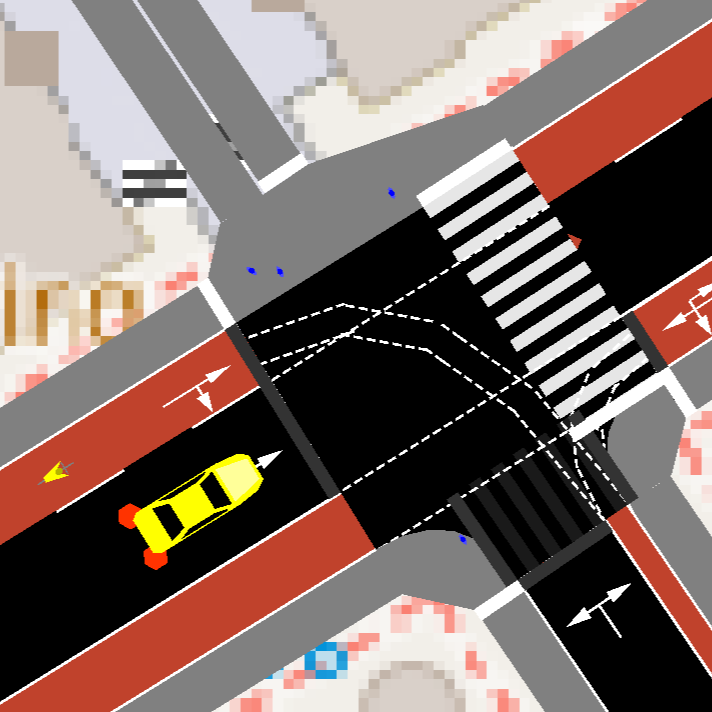
\includegraphics[width=0.48\textwidth]{images/entity_demo.png}
    \caption{Example of car, bicycle, and pedestrian entities.}
    \label{fig:entity_demo}
\end{figure}

In Figure~\ref{fig:entity_demo}, the car, travelling east, is shown as a yellow rectangle with brake lights; the bicycle, travelling east on the bicycle lane, is depicted as a yellow trapezium-like shape emerging from the left side of the image; and the pedestrians are represented as blue circles.

Route generation is controlled by several parameters, including:
\begin{itemize}
    \item \texttt{--seed}: Ensures reproducibility of the random generation process.
    \item \texttt{--insertion-density}: Controls the density of generated entities.
    \item \texttt{--binomial}: Controls how vehicle insertions are distributed over time by sampling departures from a binomial distribution.
    \item \texttt{--fringe-factor}: Ensures that vehicles spawn at the outer edges of the network.
    \item \texttt{--random-factor}: Randomizes edge weights to increase the variability between generated routes.
\end{itemize}
There are other obvious parameters omitted which allow you to specify information such as the input network for which the routes are generated, the output trip and route files, the entity type, and the start and end time of entity generation.

\subsection{Binomial Distribution}

The \texttt{--binomial} parameter allows vehicle departures to be sampled from a Binomial distribution. Real-world traffic arrivals are not perfectly periodic due to human behaviour as well as variations in the environment. Rather than inserting vehicles into the simulation at perfectly regular intervals, stochastic variation is introduced such that some seconds contain more vehicle departures and others fewer.

\[
X \sim \mathrm{Binomial}(N, p)
\]

\[
\mathbb{E}[X] = Np
\]

Where \( N \) is the number of trials given by the \texttt{--binomial} parameter, \( p \) is the probability of success, and \( Np \) equals the insertion rate calculated from the \texttt{--insertion-density} parameter. Thus, the overall expected value of departures per time step still remains equal to the deterministic insertion rate.

\begin{figure}[ht]
\centering
  \begin{subfigure}{0.49\textwidth}
  \centering
    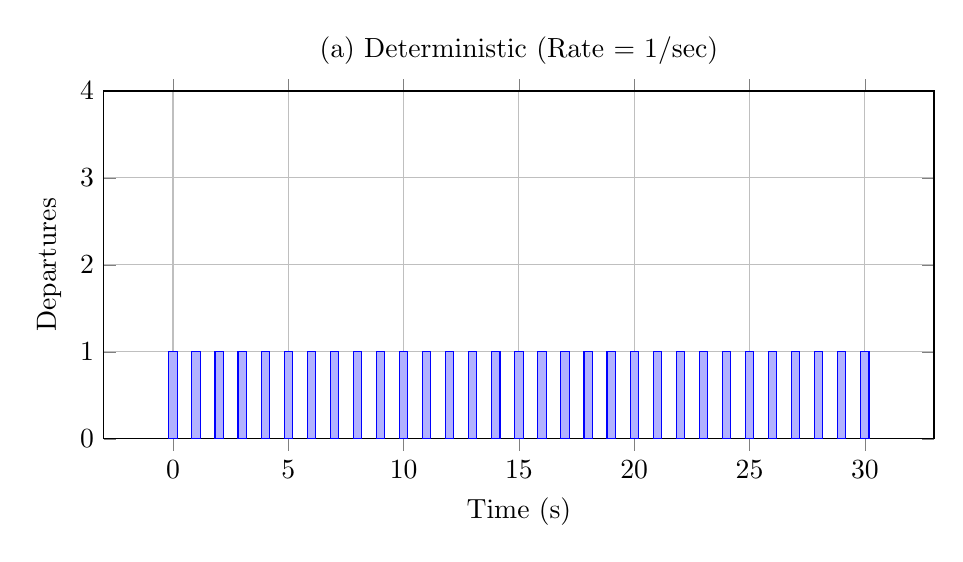
\begin{tikzpicture}
      \begin{axis}[
        width=\textwidth,
        height=6cm,
        ybar,
        bar width=3pt,
        ymin=0, ymax=4,
        xlabel={Time (s)},
        ylabel={Departures},
        title={(a) Deterministic (Rate = $1$/sec)},
        xtick={0,5,...,30},
        grid=both,
      ]
      \addplot coordinates {
        (0,1) (1,1) (2,1) (3,1) (4,1) (5,1)
        (6,1) (7,1) (8,1) (9,1) (10,1)
        (11,1) (12,1) (13,1) (14,1) (15,1)
        (16,1) (17,1) (18,1) (19,1) (20,1)
        (21,1) (22,1) (23,1) (24,1) (25,1)
        (26,1) (27,1) (28,1) (29,1) (30,1)
      };
      \end{axis}
    \end{tikzpicture}
  \end{subfigure}
  \begin{subfigure}{0.49\textwidth}
  \centering
    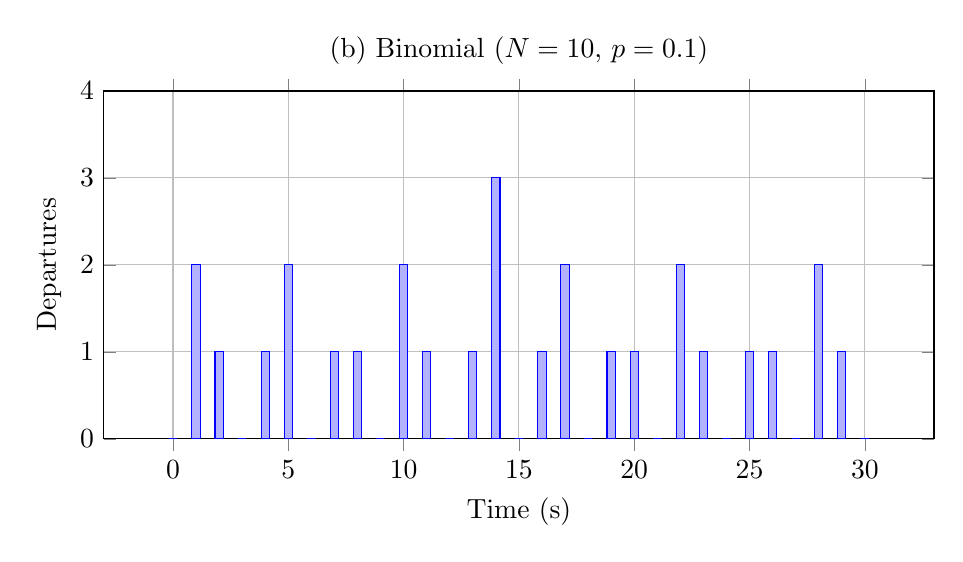
\begin{tikzpicture}
      \begin{axis}[
        width=\textwidth,
        height=6cm,
        ybar,
        bar width=3pt,
        ymin=0, ymax=4,
        xlabel={Time (s)},
        ylabel={Departures},
        title={(b) Binomial ($N=10$, $p=0.1$)},
        xtick={0,5,...,30},
        grid=both,
      ]
      \addplot coordinates {
        (0,0) (1,2) (2,1) (3,0) (4,1) (5,2)
        (6,0) (7,1) (8,1) (9,0) (10,2)
        (11,1) (12,0) (13,1) (14,3) (15,0)
        (16,1) (17,2) (18,0) (19,1) (20,1)
        (21,0) (22,2) (23,1) (24,0) (25,1)
        (26,1) (27,0) (28,2) (29,1) (30,0)
      };
      \end{axis}
    \end{tikzpicture}
  \end{subfigure}

  \caption{Comparison of deterministic and binomial vehicle insertions.}
  \label{fig:binomial_vs_deterministic}
\end{figure}

\subsection{Poisson Distribution}

In traffic theory, Poisson processes are commonly used and preferred over the Binomial distribution to model vehicle arrivals \cite{GerloughSchuhl1955}. In fact, for sufficiently large N and small p, the binomial distribution approximates a Poisson distribution:

\[
\mathrm{Binomial}(N, p) \approx \mathrm{Poisson}(\lambda),
\quad \text{where} \quad \lambda = Np
\]

The \texttt{randomTrips.py} script provides flexibility in defining vehicle traffic. For example, you may define there to be \( n \) fixed `flows' which traffic may take -- some of which may annoyingly be duplicates -- or you let any of the possible routes for the traffic be arbitrarily, independently chosen each time a new vehicle is inserted.

Whilst there is no problem with the Poisson distribution per se, the script is designed such that it is only compatible with the prior definition method. Binomial sampling on the other hand is compatible with the latter method as well as other parameters which are more flexible for our purposes and have less implementation-specific issues. For this reason, it was chosen.

\section{Summary}

This chapter described the creation of a simulated environment based on the streets surrounding UCL's Bloomsbury campus. Road network data was extracted from OpenStreetMap and refined using Google Street View. The network was implemented using SUMO, where edges and junctions were defined.

Using SUMO's \texttt{randomTrips.py} tool, there is a way for scalable creation of diverse traffic scenarios. Stochastic vehicle insertions is used to better approximate real-world traffic variability. Overall, these components establish a way in which we can train and evaluate intelligent agents.

\chapter{Reward System} \label{chapter:reward_system}

Now that we have seen how an environment -- composed of a network and traffic routes -- is constructed, we will develop a numerical reward system used to evaluate the performance of different intelligent agents. This reward system will use a contemporary traffic light system algorithm as a baseline; a good reward system is paramount to training intelligent agents effectively.

\section{Baseline Environment}

It is crucial that we understand the performance of existing traffic light systems so we can make an accurate judgement as to the benefits of our intelligent agents. Using the demo network created previously in Figure~\ref{fig:demo_simulation}, consisting of one traffic light system (TLS), three zebra crossings, and several regular crossings, we can create a baseline environment.

\subsection{Traffic Light System}

\begin{figure}[H]
    \centering
    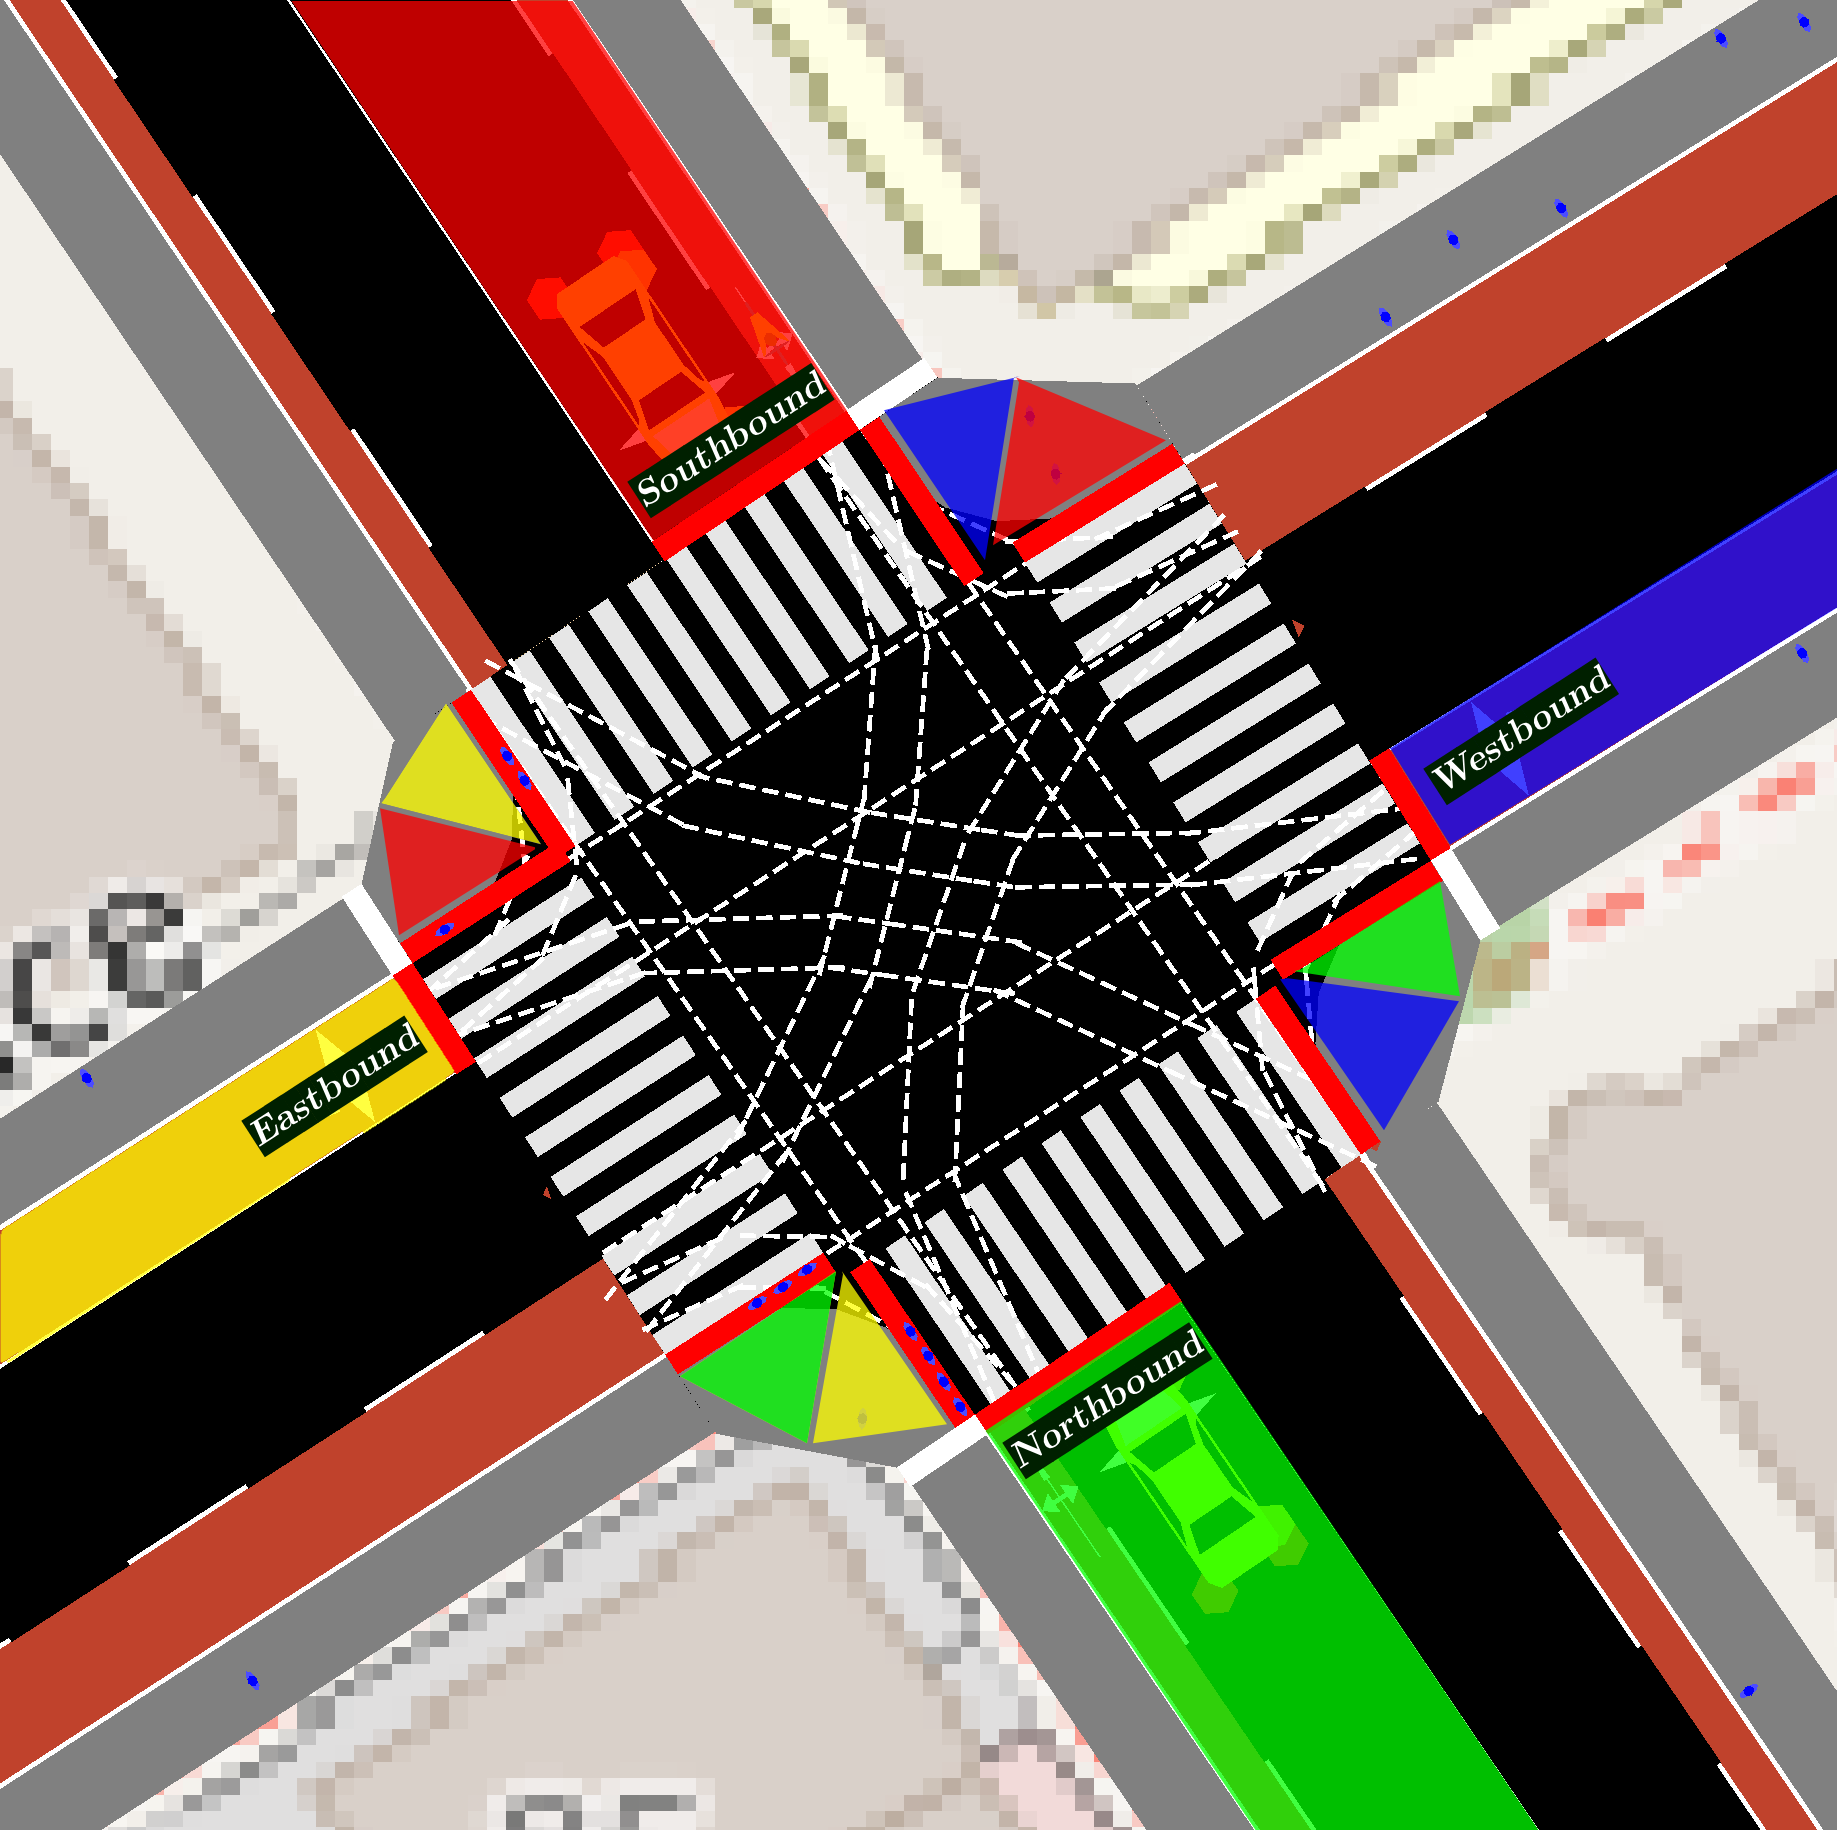
\includegraphics[width=0.48\textwidth]{images/tls_demo.png}
    \caption{Traffic Light System in the demo network.}
    \label{fig:tls_demo}
\end{figure}

In Figure~\ref{fig:tls_demo} above, green represents traffic -- including pedestrians -- that is northbound; blue represents westbound traffic; red represents southbound traffic; and yellow represents eastbound traffic.

In London, adaptive traffic light control systems are widely used enabling coordination between traffic lights -- as mentioned in our literature review. SUMO unfortunately does not support this system natively, and building a controller replica goes beyond the scope of this dissertation. Furthermore, there is only one TLS in this demo network so there wouldn't be any multi-TLS coordination regardless.

For the sake of simplicity, the TLS will use fixed-time control. The general practice is for the cycle length to be between 50 and 120 seconds, with 90 seconds often being considered optimum \cite{FHWA_SIIG04}. Below is a simple cycle striking a balance between safety and operational performance.

\begin{table}[H]
  \centering
  \begin{tabular}{c c l l}
    \hline
    \textbf{Phase} & \textbf{Duration (s)} & \textbf{Approach} & \textbf{State} \\
    \hline
    1 & 30 & Northbound/Southbound & Green \\
    2 & 3  & Northbound/Southbound & Amber \\
    3 & 2  & All approaches & Red \\
    \hline
    4 & 30 & Eastbound/Westbound & Green \\
    5 & 3  & Eastbound/Westbound & Amber \\
    6 & 2  & All approaches & Red \\
    \hline
    7 & 10 & Pedestrians & Green \\
    8 & 10 & All approaches & Red \\
    \hline
    \textbf{Total} & \textbf{90} & \\
    \hline
  \end{tabular}
  \caption{Fixed-time control phase structure.}
  \label{tab:phase_structure}
\end{table}

\subsection{Detectors}

\begin{figure}[H]
    \centering
    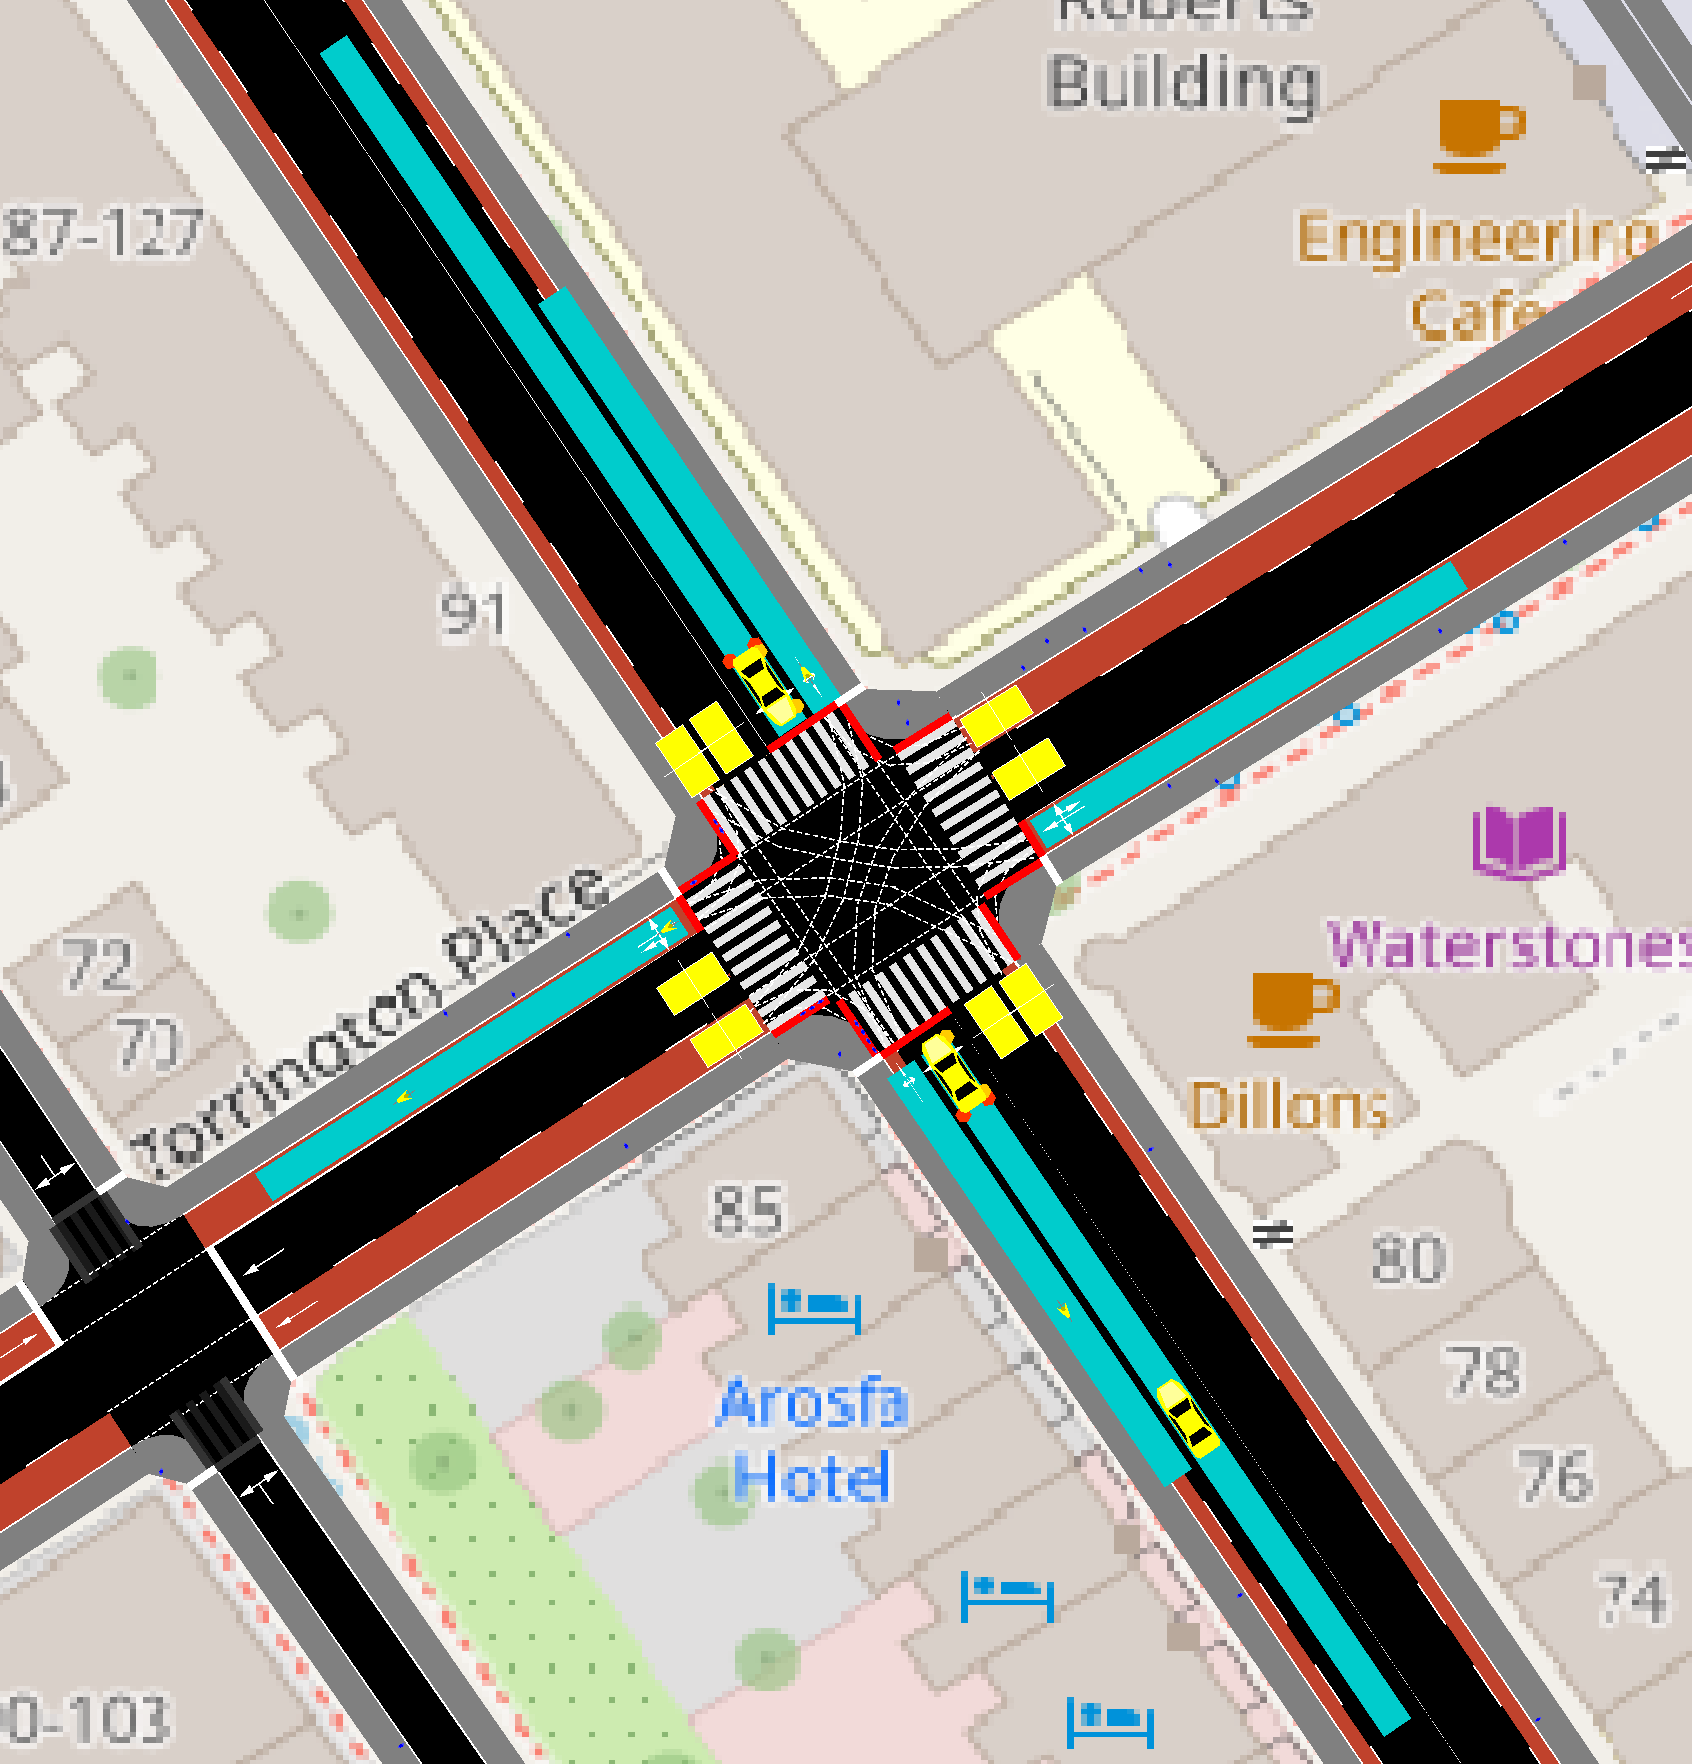
\includegraphics[width=0.48\textwidth]{images/detectors_demo.png}
    \caption{Detectors in the demo network.}
    \label{fig:detectors_demo}
\end{figure}

In Figure~\ref{fig:detectors_demo} above, the yellow-coloured detectors placed at the departure lanes are induction loops, and the aqua-coloured detectors placed at the approaches are lane area detectors.

A step length -- the time between each step -- in our simulation is defined as 1 second. After each simulation step, the detectors can be queried for information such as the vehicle count passing through them, mean speed, unique identifiers of the vehicles themselves, and time since last detection.

Induction loops have a fixed length, making them ideal for measuring vehicle throughput. Lane area detectors -- perhaps implemented as a vehicle tracking camera in reality -- can cover a larger area, making it tailored for measuring queues of traffic and keeping track of wait times.

\begin{figure}[H]
    \centering
    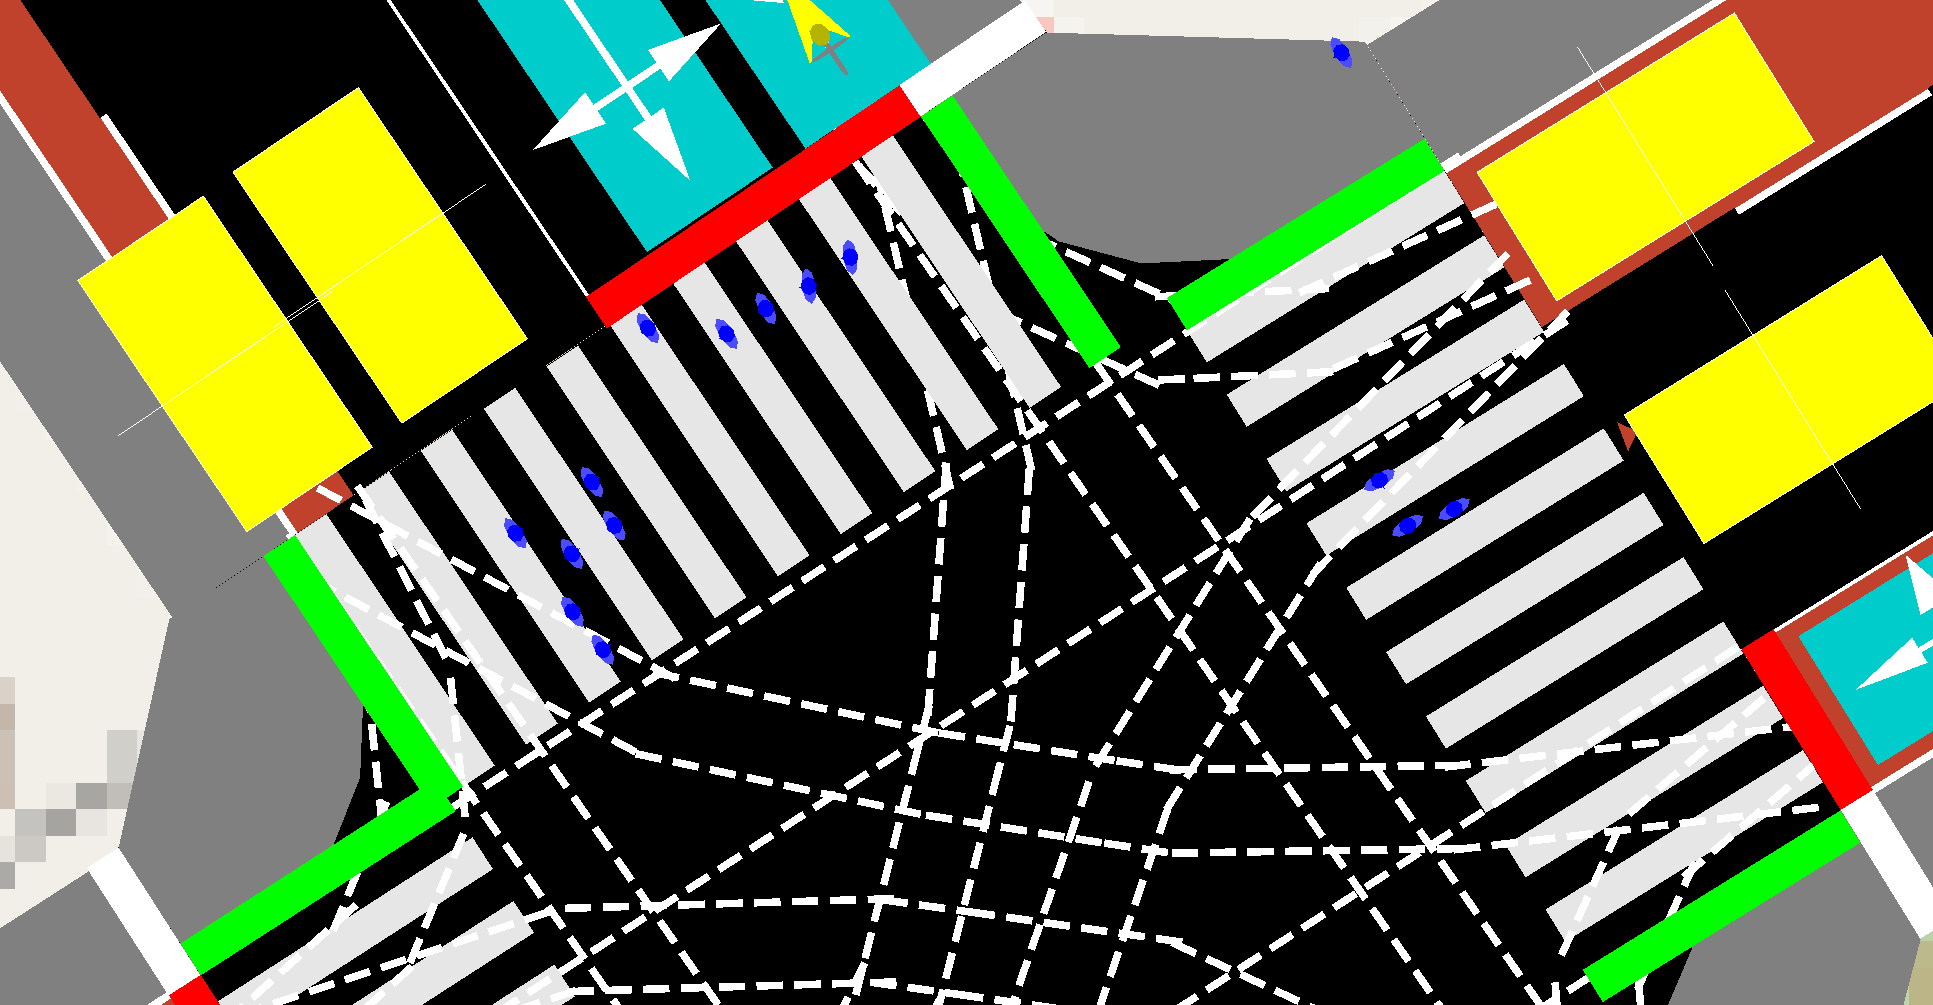
\includegraphics[width=0.48\textwidth]{images/pedestrians_demo.png}
    \caption{Example of pedestrians crossing the road.}
    \label{fig:pedestrians_demo}
\end{figure}

SUMO has no explicit support for pedestrian detectors, however a pseudo-detector can be made. To measure the queue of pedestrians waiting to use a crossing, pedestrians who are on the walking edges adjacent to the crossing are filtered such that only the pedestrians whose next walking edge is the crossing itself remain.

Pedestrians about to exit a crossing is measured by retrieving all pedestrians currently using that crossing and checking whether the remaining length of road before they finish crossing is below a threshold.

\subsection{Traffic Parameters}

In our baseline environment, the traffic densities for cars, bicycles, and pedestrians were chosen based on anecdotal observations\footnotemark\footnotetext{Not the best approach, but ``\emph{I know it when I see it}'' \cite{Stewart1964}.} that they were moderate, emulating an average day-to-day scenario -- not too light, not too dense. Furthermore, they were generated with the \texttt{--binomial} parameter set with $N=100$ to approximate a Poisson distribution as explained previously.

The \texttt{--insertion-density} parameter, which specifies the number of entities per hour per kilometer of road, was assigned for each entity type such that the traffic densities for road users, i.e.\ the cars and bicycles which use road lanes, had a combined density equivalent to pedestrians.

\begin{table}[H]
  \centering
  \begin{tabular}{l l c c}
    \hline
    \textbf{Entity} & \textbf{Type} & \textbf{Insertion Density (per hr/km)} & \textbf{Relative to Pedestrians} \\
    \hline
    Car & Road User & 100 & 0.5$\times$ \\
    Bicycle & Road User & 100 & 0.5$\times$ \\
    Pedestrian & Pavement User & 200 & 1.0$\times$ \\
    \hline
  \end{tabular}
  \caption{Comparison of the insertion density of the entities.}
  \label{tab:insertion_density_comparison}
\end{table}

It is important to note that in reality, in a dense urban environment such as London, there tends to be many more pedestrians to other road users, and there is typically more cars than bicycles. But, for the purposes of this dissertation, these nuances are ignored.

The parameters used in route generation for our baseline environment can be summarised and simplified as follows:
\begin{itemize}
    \item \texttt{--insertion-density}: 100 for cars and bicycles respectively, 200 for pedestrians $(100+100\equiv200)$.
    \item \texttt{--binomial}: $N=100$, where $N$ is the number of trials.
    \item \texttt{--fringe-factor}: Max -- vehicles are only inserted from the very edges, rather than middle of the road. Disabled for pedestrians.
    \item \texttt{--random-factor}: None -- all active edges are given equal weighting when determining which to insert a new vehicle.
\end{itemize}

\section{Reward Calculation}

Using the \texttt{randomTrips.py} script with the baseline environment and parameters defined above, we can generate traffic routes. We generate 1000 distinct routes -- each comprising of cars, bicycles, and pedestrians -- in total for the demo network, each one having a generation period of 1 hour (3600 seconds). A seed is also set for each, enumerating from 1, to ensure variability and reproducibility in the routes.

\subsection{Traffic Control Interface}

The SUMO package provides an interface that enables us to connect to our environment simulation -- called ``\emph{sumo}'' itself -- for the purposes of observation and control. Known as Traffic Control Interface (TraCI), it uses a TCP based client/server architecture, where \emph{sumo} is the server connected to by clients.

TraCI also provides a Python module of the same name, where you can create clients which connect to the environment simulation that is spun up. This is what the rest of the algorithms and systems in this dissertation will be built upon.

\begin{figure}[H]
    \centering
    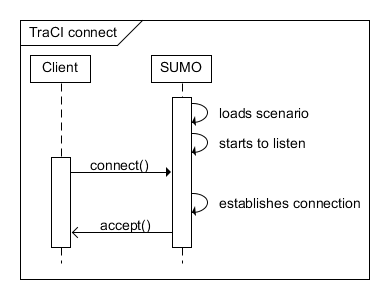
\includegraphics[width=0.48\textwidth]{images/traci_connect.png}
    \caption{TraCI: establishing a connection to SUMO \cite{TraCIProtocol26}.}
    \label{fig:traci_connect}
\end{figure}

Using TraCI, we run our baseline environment with the 1000 distinct routes generated previously in turn. For each route, the simulation is executed for 3600 seconds producing a total of $1\,000 \times 3\,600 = 3\,600\,000$ simulation steps across all runs.

\subsection{Reward Formula}

The reward formula combines four measurable indicators of traffic performance into a single scalar value that can be used to evaluate performance, and can be optimised by an intelligent agent. They are as follows, calculated using the aforementioned detectors queried using TraCI:
\begin{itemize}
  \item $z_{vd}$: Total vehicle delay
  \item $z_{vt}$: Total vehicle throughput
  \item $z_{pd}$: Total pedestrian delay
  \item $z_{pt}$: Total pedestrian throughput
\end{itemize}

Delay is defined as the continuous time (seconds) in which vehicles or pedestrians in the detection area have had a speed of less than 0.1 m/s, indicating waiting. Vehicle throughput is defined as the number of vehicles crossing the departure detectors; pedestrian throughput is defined as the number of pedestrians finishing using their crossing.

At time step $t$, the reward $R_t$ can be expressed as a weighted sum of the four metrics: 

\begin{equation}
  \label{reward_formula}
  R_t =
  w_{vd}(-z_{vd}) +
  w_{vt}(z_{vt}) +
  w_{pd}(-z_{pd}) +
  w_{pt}(z_{pt}) +
  P_t
\end{equation}

Where the coefficients, or weights rather, $w_{vd}$, $w_{vt}$, $w_{pd}$, and $w_{pt}$ determine the relative importance of each metric. Delay terms are negated since increased delay represents worse performance. $P_t$ is a penalty applied.

\subsection{Penalty}

At any given step in our simulation, if a vehicle is \emph{teleported} to their next edge in the simulation, or out of the simulation entirely, a penalty will be occurred of $-1000.0$ units. This was chosen as it is non-insignificant relative to the average reward per step (when step length is $1$ second).

Teleports ensure that any vehicle that is stuck -- due to a grid-lock or being jammed -- or simply waiting too long is moved along to allow for other entities to progress normally. Occasionally, two vehicles may unfortunately `collide', unable to decide who should be prioritised and who should yield due to problems with SUMO itself.

\begin{figure}[H]
    \centering
    \begin{subfigure}{0.48\textwidth}
        \centering
        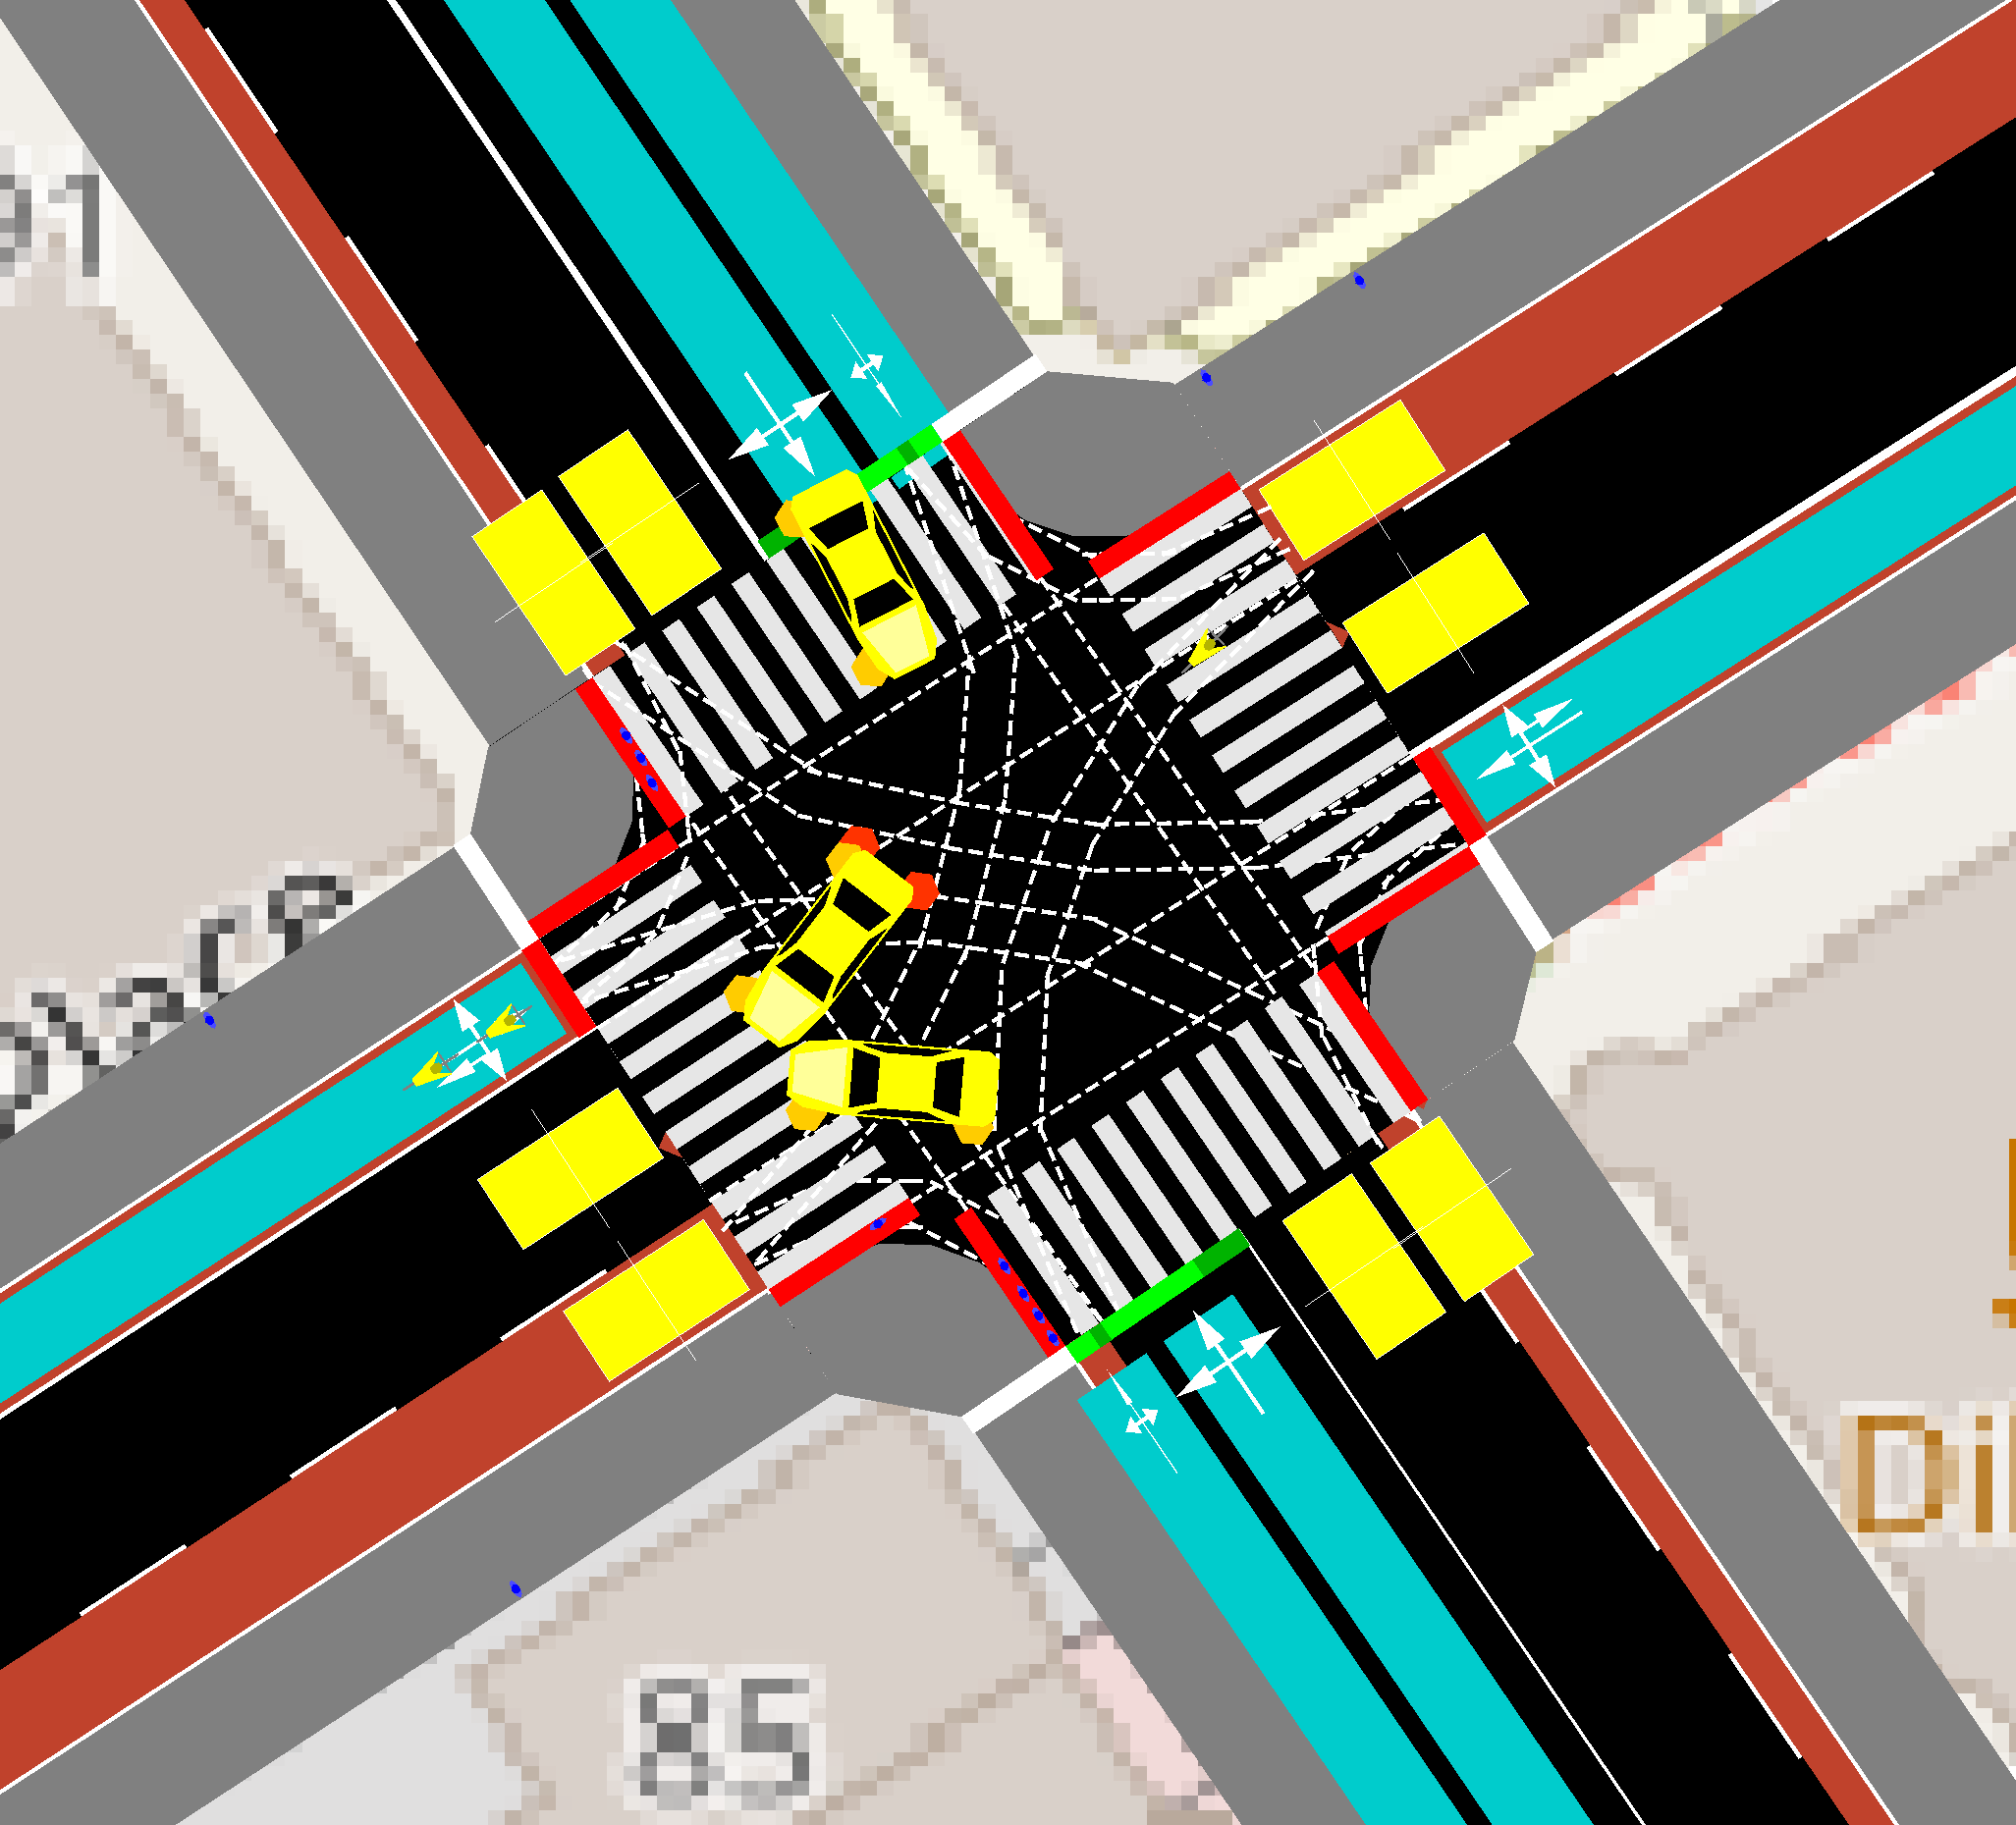
\includegraphics[width=\textwidth]{images/collision_begin_demo.png}
        \caption{Collision starts during step $1726$.}
        \label{fig:demo_collision_beign}
    \end{subfigure}
    \hfill
    \begin{subfigure}{0.48\textwidth}
        \centering
        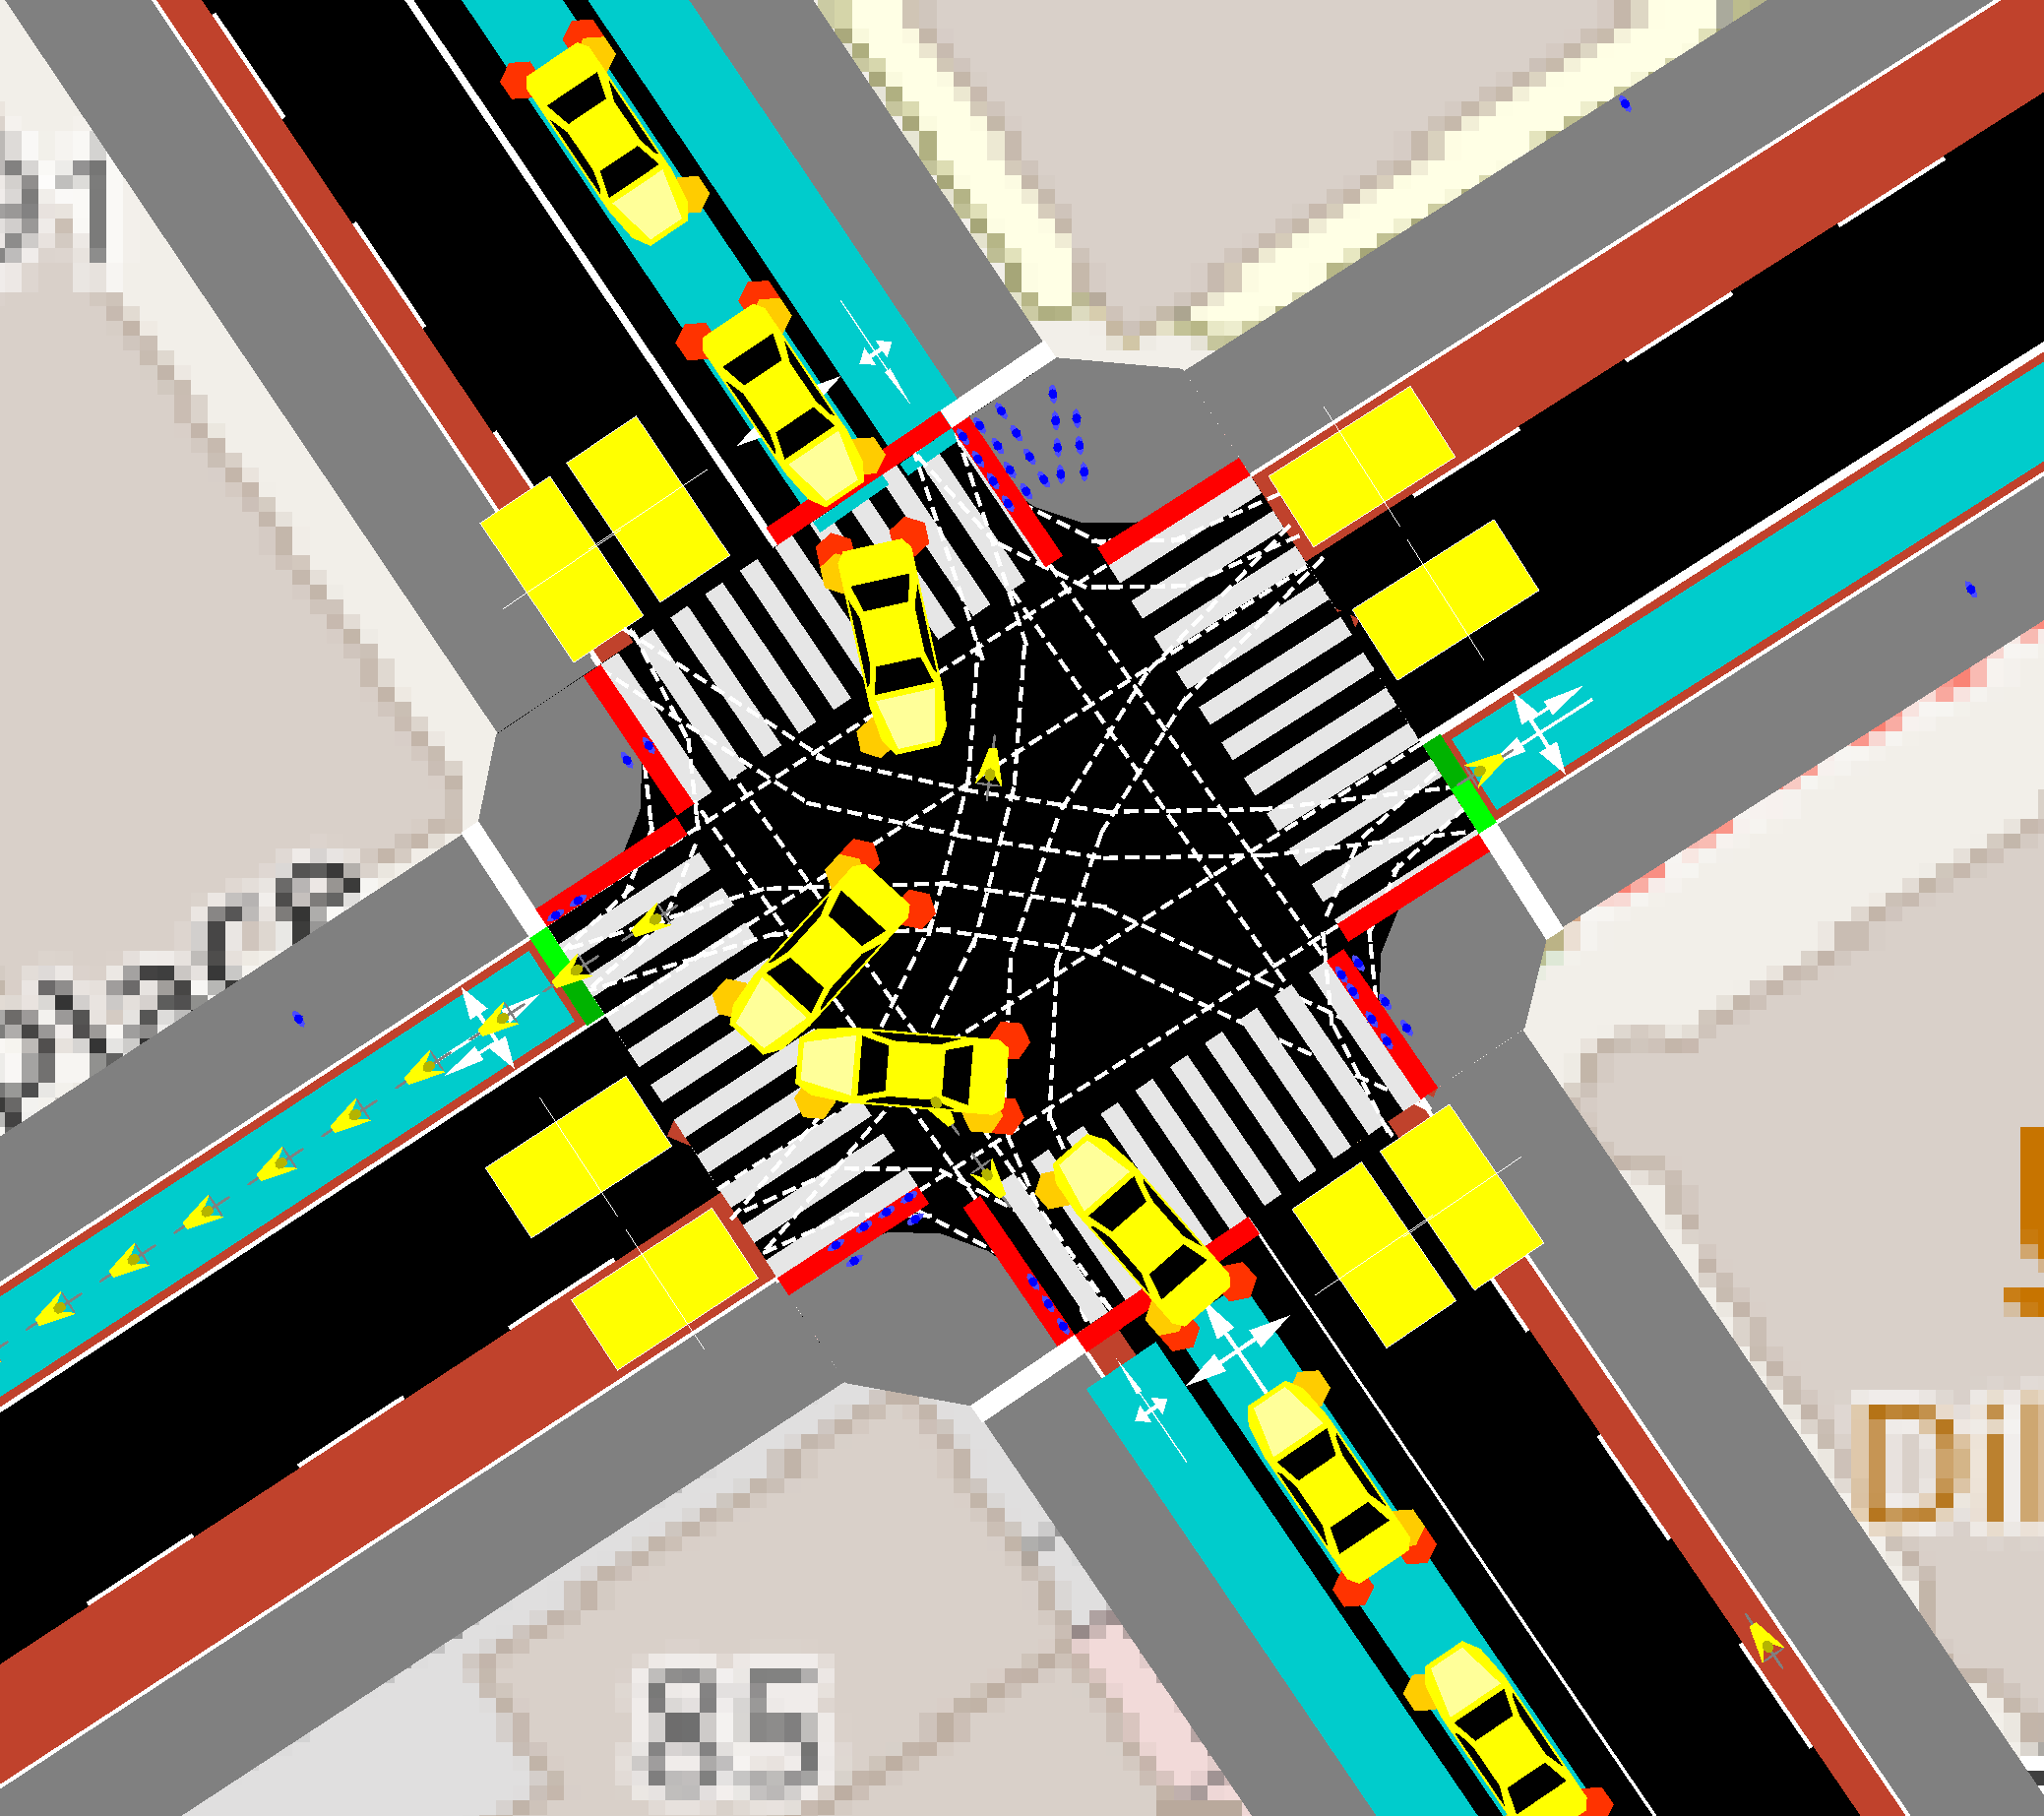
\includegraphics[width=\textwidth]{images/collision_end_demo.png}
        \caption{Just before teleportations during step $2026$.}
        \label{fig:demo_collision_end}
    \end{subfigure}
    \caption{Collision example in the $811$th generated route, lasting $300$ steps.}
    \label{fig:demo_collision}
\end{figure}

The issue in Figure~\ref{fig:demo_collision} is as an artefact of setting the step length to a value of $1$ second. Vehicles are only able to make judgements every second leading to high reactions times and sometimes sub-optimal choices. Here, two vehicles are seen trying to progress to the same position, arriving at the exact same second, and from practically the same distance, leading to the simulation unable to resolve priority.

This may be resolved by setting the step length to $0.1$ seconds, allowing arrival measurements to be taken with sub-second precision making it easier to identify who should yield. However the $\sim10\times$ increase in simulation time to resolve a problem that occurs rarely was not deemed a worthwhile tradeoff.

\subsection{Weights}

The four metric values $z_{vd}$, $z_{vt}$, $z_{pd}$, and $z_{pt}$ are calculated per each of the 3\,600\,000 simulation steps and then cached inside of a buffer with four columns. Once the final route has finished running, we can use the \texttt{numpy} Python module to calculate statistics regarding each metric stored within the buffer.

\begin{table}[H]
  \centering
  \begin{tabular}{lrrrrr}
    \hline
    \textbf{Metric} & \textbf{Mean} & \textbf{Standard Deviation} & \textbf{Min} & \textbf{Max} & \textbf{Sum} \\
    \hline
    $z_{vd}$ & 63.07 & 67.07 & 0 & 5032 & 227066504 \\
    $z_{vt}$ & 0.235 & 0.515 & 0 & 5 & 844528 \\
    $z_{pd}$ & 211.69 & 220.43 & 0 & 1702 & 762082178 \\
    $z_{pt}$ & 0.252 & 1.199 & 0 & 21 & 908941 \\
    \hline
  \end{tabular}
  \caption{Summary statistics for vehicle and pedestrian metrics (runtime: 3:16:02).}
  \label{summary_statistics}
\end{table}

These metrics are not for a single vehicle or pedestrian, but rather it is based on the cumulative value for all vehicles or pedestrians that are on the detectors at a given simulation step.

Since the fixed-time control TLS will serve as the baseline against which we evaluate our intelligent agents, the weights in formula \eqref{reward_formula} are adjusted based on the summary statistics in Table~\ref{summary_statistics} above. Namely, each of the weights are normalised using the mean value for the corresponding metric such that the average calculated reward for the fixed-time control TLS is a baseline of 0.

\begin{itemize}
  \item $w_{vd}$: $\frac{1}{63.07}=0.01586$
  \item $w_{vt}$: $\frac{1}{0.235}=4.255$
  \item $w_{pd}$: $\frac{1}{211.69}=0.004724$
  \item $w_{pt}$: $\frac{1}{0.252}=3.968$
\end{itemize}

If we calculate the reward after each of the 1000 routes is run using the fixed-control TLS, we confirm that the average calculated reward is about 0.

The 3 visible spikes in the graph correspond to routes in which teleportations occurred incurring penalties. Although not ideal, they are indeed rare and do not effect the final result significantly. Penalties will be a useful feature which discourage actions by our traffic light agents that cause vehicles to wait inordinately long.

\begin{figure}[H]
  \centering
  \begin{tikzpicture}
  \begin{axis}[
      width=14cm,
      height=8cm,
      xlabel={Route},
      ylabel={Reward},
      title={Baseline environment reward per route},
      grid=both,
  ]

  \addplot[
      blue,
      mark=none
  ] table[
      x expr=\coordindex+1,
      y index=0
  ] {data/demo_train_ft.txt};
  \addlegendentry{Fixed-time control}

  \end{axis}
  \end{tikzpicture}
  \caption{Reward per route using a fixed-time control TLS.}
\end{figure}

Equal weighting is currently given to pedestrians and road users (cars and bicycles) as a consequence of the traffic parameters mentioned previously for our baseline environment and the current reward formula. Neither is implicitly being prioritised over the other.

Although not explored further in this dissertation, an interesting extension would be to vary the weights to prioritise either pedestrians or vehicles. For example, vehicles may reasonably be assigned a slightly higher priority considering that cars in England have an average occupancy of approximately 1.57 persons per \cite{StatistaCarOccupancy}. However, this may conflict with broader urban plans of encouraging walking and improving pedestrian safety.

\section{Summary}

This chapter explored the creation of a baseline environment that incorporates a fixed-control traffic light system as well as well defined traffic parameters. To observe car, bicycle, and pedestrian traffic, a set of detectors was deployed.

Using the TraCI interface, a way for controlling and observing the simulation environment was created. This also enabled a weighted reward formula to be defined and calculated. Both of which will be crucial for our following intelligent agents.

\chapter{Q-Learning} \label{chapter:q_learning}

Having created a baseline environment with a traffic light system which can be observed and controlled, as well as creating a reward system, we now create the first of our intelligent agents. These agents are \emph{decentralised}, relying only on data from the local traffic light system. Reinforcement learning and the Markov decision process will first be briefly explained before implementing the Q-learning algorithm. The performance and possible improvements will then be considered.

\section{Background}

Reinforcement learning relates to how an intelligent agent should take actions in a dynamic environment to maximise a reward. The Reward Hypothesis states that ``\emph{all of what we mean by goals and purposes can be well thought of as maximization of the expected value of the cumulative sum of a received scalar signal (reward)}''\cite{RichardSutton1990}.

Thereby the goal of our agents may be formally defined as selecting optimal actions based on the state of the SUMO environment to maximise total future reward defined by formula \eqref{reward_formula}.

\subsection{State} \label{q_learning_state}

For each time step in our environment simulation, for each traffic light system (TLS), the state can be broadly split into three sections: the current traffic light phase of the TLS, the number of vehicles currently using the lanes controlled by the TLS, and the number of pedestrians currently in the pavement waiting areas of the TLS.

Consider our demo network created previously. We can annotate the TLS with the different components which constitute the state as shown below.

\begin{figure}[H]
    \centering
    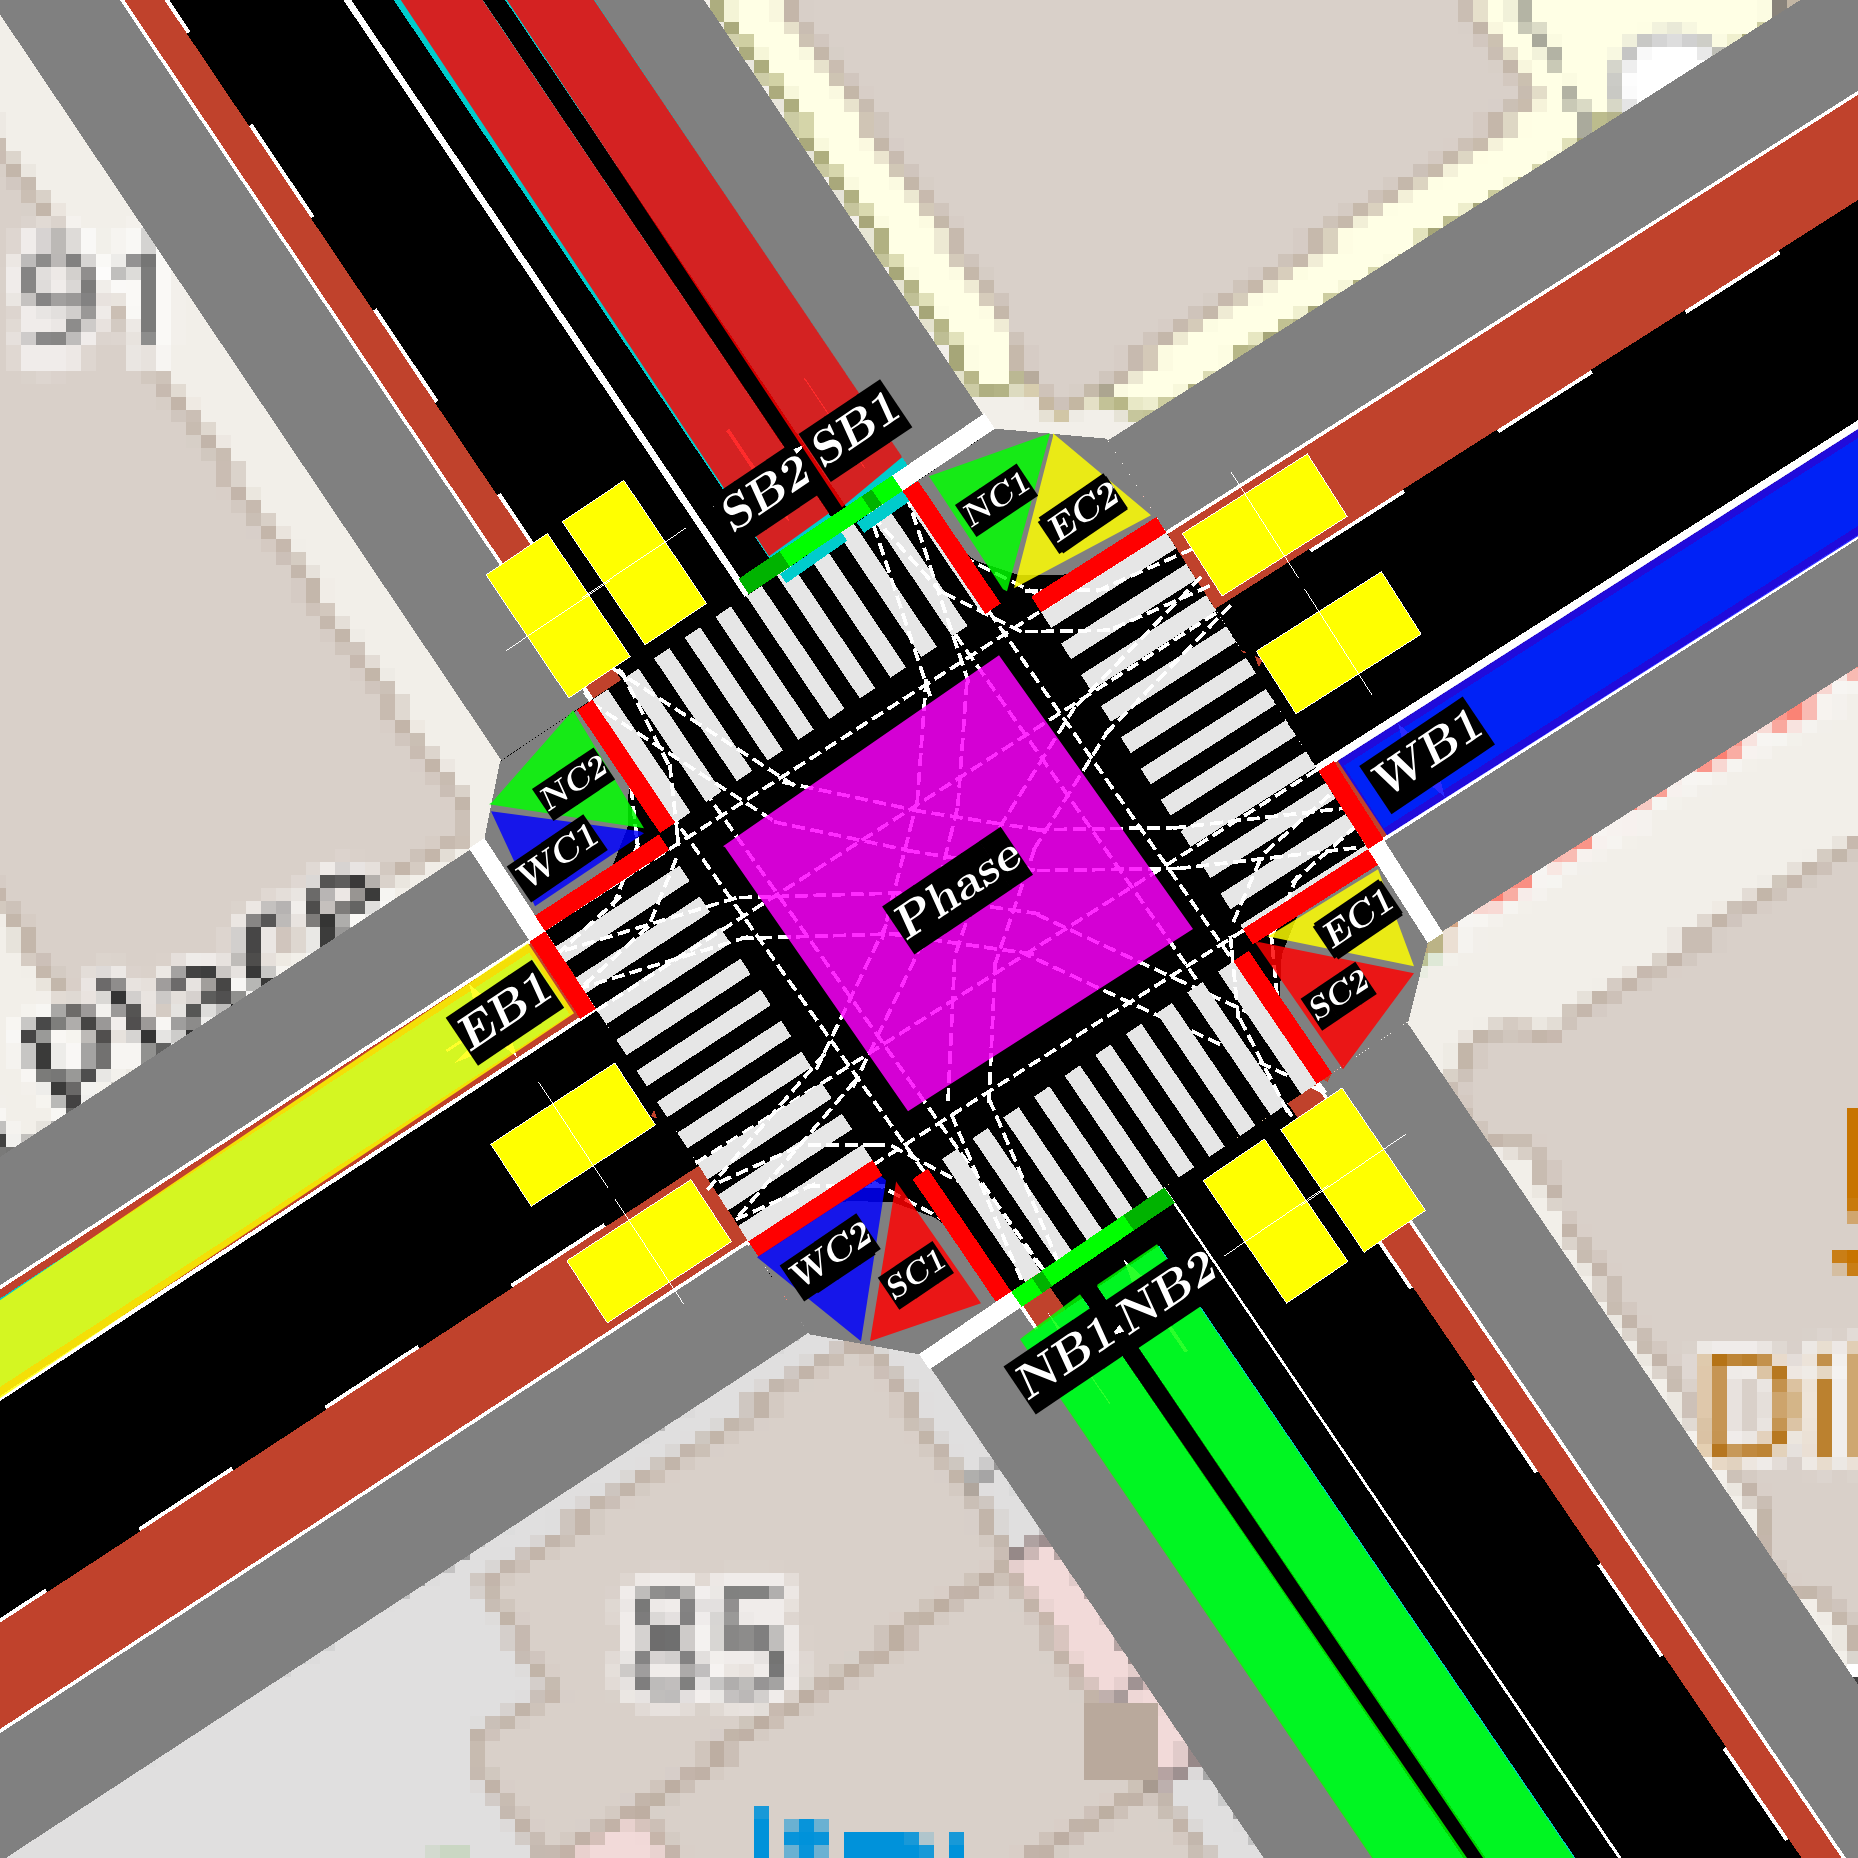
\includegraphics[width=0.48\textwidth]{images/state_demo.png}
    \caption{Annotated state in the demo network.}
    \label{fig:state_demo}
\end{figure}

In Figure~\ref{fig:state_demo} above, the labels with prefix `\emph{N}' means \emph{north}, `\emph{E}' means \emph{east}, `\emph{S}' means \emph{south} and `\emph{W}' means \emph{west}.

If the cardinal direction \emph{X} is followed by letter `\emph{B}', the label should be interpreted as \emph{X-bound}, e.g.\ `\emph{NB1}' should read as the number of vehicles in the \emph{first}, or rather, leftmost lane travelling \emph{northbound}. In this instance, there are two lanes going northbound, one being a dedicated bicycle lane. If \emph{X} is instead followed by letter `\emph{C}', the label should be interpreted as \emph{X-crossing-wait-area}, e.g.\ `\emph{SC2}' should read as the number of pedestrians in the \emph{second} of the two \emph{wait area} for the \emph{south} \emph{crossing}. Finally, the `\emph{Phase}' label reflects the current traffic light phase of the TLS.

For this particular TLS, the state is comprised of 15 parts, therefore it can be encoded as an $n$-tuple where $n$ is $15$. Generalising this idea, we can write the full uncompressed state $S$ at time $t$ for any TLS\footnotemark\footnotetext{In some TLS it may be hard to define a relative cardinal direction, e.g.\ for a single crossing in a two-way road, or for an exit lane in a roundabout with more than 4 exits. In such cases it would be desirable to use an alternative naming scheme for state variables.} as follows.

\[
  Veh_t = (NB_1, ..., NB_a, WB_1, ..., WB_b, SB_1, ..., SB_c, EB_1, ..., EB_d)
\]
\[
  Ped_t = (SC_1, SC_2, WC_1, WC_2, NC_1, NC_2, EC_1, EC_2)
\]
\begin{equation}
  \label{state_formula}
  S_t = (Phase_t,) + Veh_t + Ped_t
\end{equation}

Where \emph{a}, \emph{b}, \emph{c}, and \emph{d} are the number of lanes going northbound, westbound, southbound, and eastbound respectively. Note that in some cases, the $Veh_t$ (vehicles) and $Ped_t$ (pedestrians) tuples may not contain an entry for some lanes or crossings listed depending on the TLS topology.

\subsection{Actions}

Recall Table~\ref{tab:phase_structure} in which we defined the fixed-time control phase structure. Phases 1--3 of the TLS related to the northbound/southbound approaches, phases 4--6 related to the eastbound/westbound approaches, and phases 7--8 related to the collective pedestrian approaches of the TLS.

We will formally define an action to be one which switches -- or maintains -- the approach that is currently active. The three actions will be switching to phase 1, switching to phase 4, or switching to phase 7. The rest of the phases are \emph{not} viable switches that can be made directly by the agent. Rather, these will be considered \emph{phase switch} actions mapped to a particular action.

\begin{table}[H]
  \centering
  \begin{tabular}{c c c c}
    \hline
    \textbf{Action Index} & \textbf{TLS Phase} & \textbf{Duration (s)} & \textbf{Phase Switch} \\
    \hline
    0 & 1 & 30 & (2, 3 s) $\to$ (3, 2 s) \\
    \hline
    1 & 4 & 30 & (5, 3 s) $\to$ (6, 2 s) \\
    \hline
    2 & 7 & 10 & (8, 10 s) \\
    \hline
  \end{tabular}
  \caption{Traffic light system actions in the demo network.}
  \label{tab:phase_actions}
\end{table}

A phase switch contains one or more tuples of the format (\emph{phase}, \emph{duration (s)}). These phases must be sequentially run when switching \emph{away} from the current TLS phase. Suppose the current phase is 1 (index 0) which has finished execution. If the next action taken is to switch to phase 4 (index 1), the phase switch (2, 3 s) $\to$ (3, 2 s) first executes. That is the phase is set to 2 for 3 seconds, followed by phase 3 for 2 seconds. Finally, phase 4 runs as intended.

Phase switch allows for a smooth transition between traffic flow directions, giving a buffer of time in which vehicles or pedestrians can finish their travels safely (by transitioning the traffic lights to yellow then red). It is \emph{not} applied if going from the current action index to itself.

\subsection{Markov Decision Process}

A Markov Decision Process (MDP) is a mathematical model for sequential decision making when outcomes are uncertain. Formally, a MDP can be defined as a 5-tuple ($S$, $A$, $P_a$, $R_a$, $\gamma$), where:

\begin{itemize}
  \item $S$ is a set of \textbf{states} called the state space. In our demo network, it is every valid possible configuration of our $S_t$ tuple before and after an action is taken.
  \item $A$ is a set of \textbf{actions} called the action space. This would be the 3 action indexes we defined previously.
  \item $P_a(s,s')$ is the transition \textbf{probability} that action $a$ in state $s$ at time $t$ will lead to state $s'$ at time $t+1$. This will not be known or estimated by our agents since Q-learning is \emph{model-free}.
  \item $R_a(s,s')$ is the \textbf{reward} received after action $a$ is taken to transition from state $s$ to $s'$. This is the cumulative sum of $R_t$ over the duration of the action.
  \item $\gamma$ is the \textbf{discount factor} between $0 \leq \gamma \leq 1$ which determines how much future rewards matter.  
\end{itemize}

The MDP is used to model the stochastic (i.e.\ involving random probability) process in which our intelligent agents try to find an optimal policy $\pi^*$, where a policy is some function $\pi$ which maps a state $s$ to an action $a$: $\pi(s)=a$. The optimal policy $\pi^*$ should maximise expected cumulative reward:

\[
E\left[\sum_{t=0}^{\infty}\gamma^t{R_a}_t(s_t,s_{t+1})\right]
\]

An summary overview of the MDP can be given as follows:

\begin{figure}[H]
  \centering
  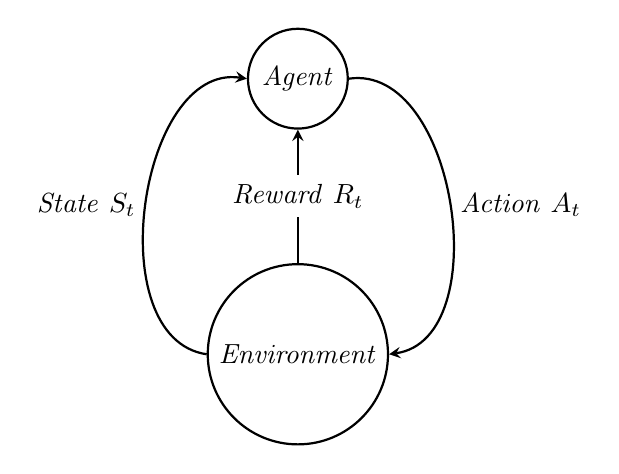
\begin{tikzpicture}[node distance=3.5cm]
    \tikzset{state/.style = {circle, draw=black, thick}}
    \tikzset{arrow/.style = {>=stealth, thick}}
    \node[state] (agent) {\emph{Agent}};
    \node[state] (env) [below of=agent] {\emph{Environment}};
    \draw[->, bend left=90, arrow] (agent) to node[right]{\emph{Action} $A_t$} (env);
    \draw[<-, bend right=90, arrow] (agent) to node[left]{\emph{State} $S_t$} (env);
    \draw[<-, arrow] (agent) to node[midway, fill=white]{\emph{Reward} $R_t$} (env);
  \end{tikzpicture}
  \caption{Markov Decision Process overview.}
  \label{fig:markov_decision_process}
\end{figure}

Pedantically, we actually use a Semi-Markov Decision Process (SMDP). Unlike standard MDPs, SMDPs enable actions to have a variable duration as seen in Table~\ref{tab:phase_actions} as opposed to being instant -- occurring in a single step. This distinction is accommodated in our later equations.

\section{Q-Learning}

Q-learning is a specific reinforcement learning algorithm used to find the optimal policy within a Markov Decision Process. It trains an agent to assign values to its possible actions based on its current state, without requiring a model of the environment (model-free, i.e.\ the transition probabilities are not known).

``\emph{Q}'' refers to the function that the algorithm computes: the quality -- that is, the expected reward -- of an action taken in a given state.

\[
Q: S \times A \to \mathbb{R}
\]

This function can be used to construct a tabular representation known as a Q-table, which enumerates every possible combination of state and action and maps it to a corresponding quality value, set to any arbitrary value initially (we choose 0).

\begin{figure}[H]
  \centering
  \[
  Q(s, a) =
  \begin{array}{c|ccc}
    \text{} & a=0 & a=1 & a=2 \\
    \hline
    s_1 & Q(s_1,0) & Q(s_1,1) & Q(s_1,2) \\
    s_2 & Q(s_2,0) & Q(s_2,1) & Q(s_2,2) \\
    s_3 & Q(s_3,0) & Q(s_3,1) & Q(s_3,2) \\
    \vdots & \vdots & \vdots & \vdots \\
    s_n & Q(s_n,0) & Q(s_n,1) & Q(s_n,2) \\
    \vdots & \vdots & \vdots & \vdots \\
  
  \end{array}
  \]
  \caption{Example of Q-table with $n$ states and 3 actions.}
  \label{arr:q_table_example}
\end{figure}

After running Q-learning -- outlined below -- over many episodes, the values in the Q-table converge towards their optimal estimates. Once this happens, the optimal policy $\pi^*$ can be derived from the Q-table directly:

\begin{enumerate}
  \item For any given state, select the action with the highest quality value.
  \item Execute this action to transition to the next state.
  \item Repeat this process at each subsequent state.
\end{enumerate}

\subsection{Algorithm}

\begin{algorithm}[H]
  \caption{Tabular Q-Learning}
  \begin{algorithmic}[1]
  \State Initialise $Q(s,a) = 0$ for all $s \in S, a \in A$
  \For{each episode}
      \State Observe state $s$ from environment
      \For{each step in episode}
          \State Choose action $a$ using policy $\pi$
          \State Execute action $a$
          \State Observe cumulative reward $R$, next state $s'$, and duration $d$
          \State $Q(s,a) \leftarrow Q(s,a) + \alpha \Big(R + \gamma^d \underset{a'}{\max} Q(s',a') - Q(s,a)\Big)$
          \State Set $s \leftarrow s'$
      \EndFor
  \EndFor
  \end{algorithmic}
\end{algorithm}

In line 5, the training policy $\pi$ we will use to choose an action is called \emph{$\epsilon$-greedy}, explained later. This training policy is distinct from the optimal policy $\pi^*$ described earlier.

When we execute the chosen action $a$ from state $s$ and observe the cumulative reward $R$, next state $s'$, and duration $d$ of the action, $Q(s,a)$ is updated as shown in line 8 as follows:

\[
  Q(s,a) + \alpha \Big(R + \gamma^d \underset{a'}{\max} Q(s',a') - Q(s,a)\Big)
\]

Where $\alpha$ is the learning rate, and $\gamma$ is the discount factor. Since this is a SMDP rather than a standard MDP, we add the exponent $d$ to the $\gamma$ term to account for duration.

$\alpha$ determines to what extent new information overrides old. A factor of 0 makes the existing value not update at all, whereas a value of 1 makes the agent consider only the most recent information. We use the standard value of $\alpha=0.1$ since actions in the traffic environment are not fully deterministic.

$\gamma$ determines the importance of future rewards. A factor of 0 makes the agent only consider current rewards, while a factor approaching 1 encourages long-term high reward. It may seem obvious to choose a factor very close or equal to 1, however action values may become unstable or diverge to infinity. Ergo, $\gamma=0.9$ was chosen.

$\underset{a'}{\max} Q(s',a')$ should read as an estimate of the optimal future value. It returns the maximum quality value over all actions $a'$ possible from the next state $s'$.

\subsection{Decaying $\epsilon$-greedy policy}

At the start, our Q-table will not be populated with values such that trying to follow the optimal policy will lead to an optimal strategy. We need a way to initially \emph{explore} actions to discover what works best, before eventually choosing to \emph{exploit} the best actions found.

The $\epsilon$-greedy (epsilon-greedy) policy works by generating a random number $r\in[0,1]$ at each time step during training. When our Q-learning algorithm then selects an action, with probability $\epsilon$ (i.e.\ if $r < \epsilon$) it will explore and choose uniformly at random one of the 3 actions, otherwise with probability $1-\epsilon$ it will exploit and choose the best action `greedily'.

\begin{table}[H]
  \centering
  \begin{tabular}{c | l l l}
    \textbf{} & a=0 (\emph{best}) & a=1 & a=2 \\
    \hline
    $\epsilon=0.1$ & \makecell[l]{0.9000 +\\0.3333 =\\0.9333} & 0.3333 & 0.3333 \\
  \end{tabular}
  \caption{Example action probability table, where $a=0$ is the best.}
  \label{tab:action_probabilities}
\end{table}

Too much exploitation may result in our agent getting stuck with a suboptimal strategy. Too much exploration may result in our agent wasting time trying random actions and never settling on a good solution.

To make the epsilon value start high and lessen as training goes on, we define epsilon $\epsilon$ to be a function which exponentially decays with every time step $t$.

\[
  \epsilon(t) = \epsilon_{min} + (\epsilon_{max}-\epsilon_{min}) e^{-\lambda t} 
\]

\pgfmathsetmacro{\emin}{0.01}
\pgfmathsetmacro{\emax}{1}
\pgfmathsetmacro{\decay}{0.0000015}
\pgfmathsetmacro{\episodes}{3600000}

\begin{figure}[H]
  \centering
  \begin{tikzpicture}
    \begin{axis}[
        xlabel={$t$},
        ylabel={$\epsilon(t)$},
        domain=0:\episodes,
        grid=both,
    ]
    \addplot[
        black,
        thick
    ]
    {\emin + (\emax - \emin)*exp(-\decay*x)};
    \end{axis}
  \end{tikzpicture}
  \caption{Epsilon exponential decay graph.}
  \label{fig:epsilon_decay}
\end{figure}

Where $\epsilon_{min}$ is the minimum epsilon value (set to $0.01$) to ensure randomness remains later on in the learning phase, $\epsilon_{max}$ is the starting epsilon value (set to $1$), and $\lambda$ is the decay rate constant (set to $1.5\times10^{-6}$).

The constants were chosen empirically\footnotemark\footnotetext{Multiple parameters were tested using the \emph{Desmos} web-based graphing calculator \cite{DemosGraphingCalculator}.} such that the graph decays smoothly over time to about $0.01$ by the time step $3\,600\,000$ -- the total number of training steps across all episodes -- is reached.

\subsection{Implementation}

Previously, we created a route generation script in Python to call the \texttt{randomTrips.py} tool with varying traffic parameters several times automatically, to create 1000 baseline environment routes in our file system.

Most of our other code was placed within a custom \texttt{Environment} library which utilises a TraCI connection to the actual SUMO environment. This library has an \emph{exposed} interface including, but not limited to:

\begin{itemize}
  \item Setting the current road network and entity route files.
  \item Getting the current full uncompressed state via the detectors.
  \item Calculating the weighted reward formula.
  \item A \texttt{Controller} for performing actions on a particular traffic light system.
\end{itemize}

Now we establish an \texttt{Agents} library in which our algorithm implementations and code for setting up agents and training will lie. Firstly, an abstract \texttt{Runner} class is created with a one-to-one mapping to a \texttt{Controller} which it runs. We then create two classes for now that implement the abstract class: a \texttt{DefaultRunner} class (representing the baseline fixed-time control), and a \texttt{QLearning} class that implements the Q-learning algorithm in an object-oriented manner.

\begin{figure}[H]
    \centering
    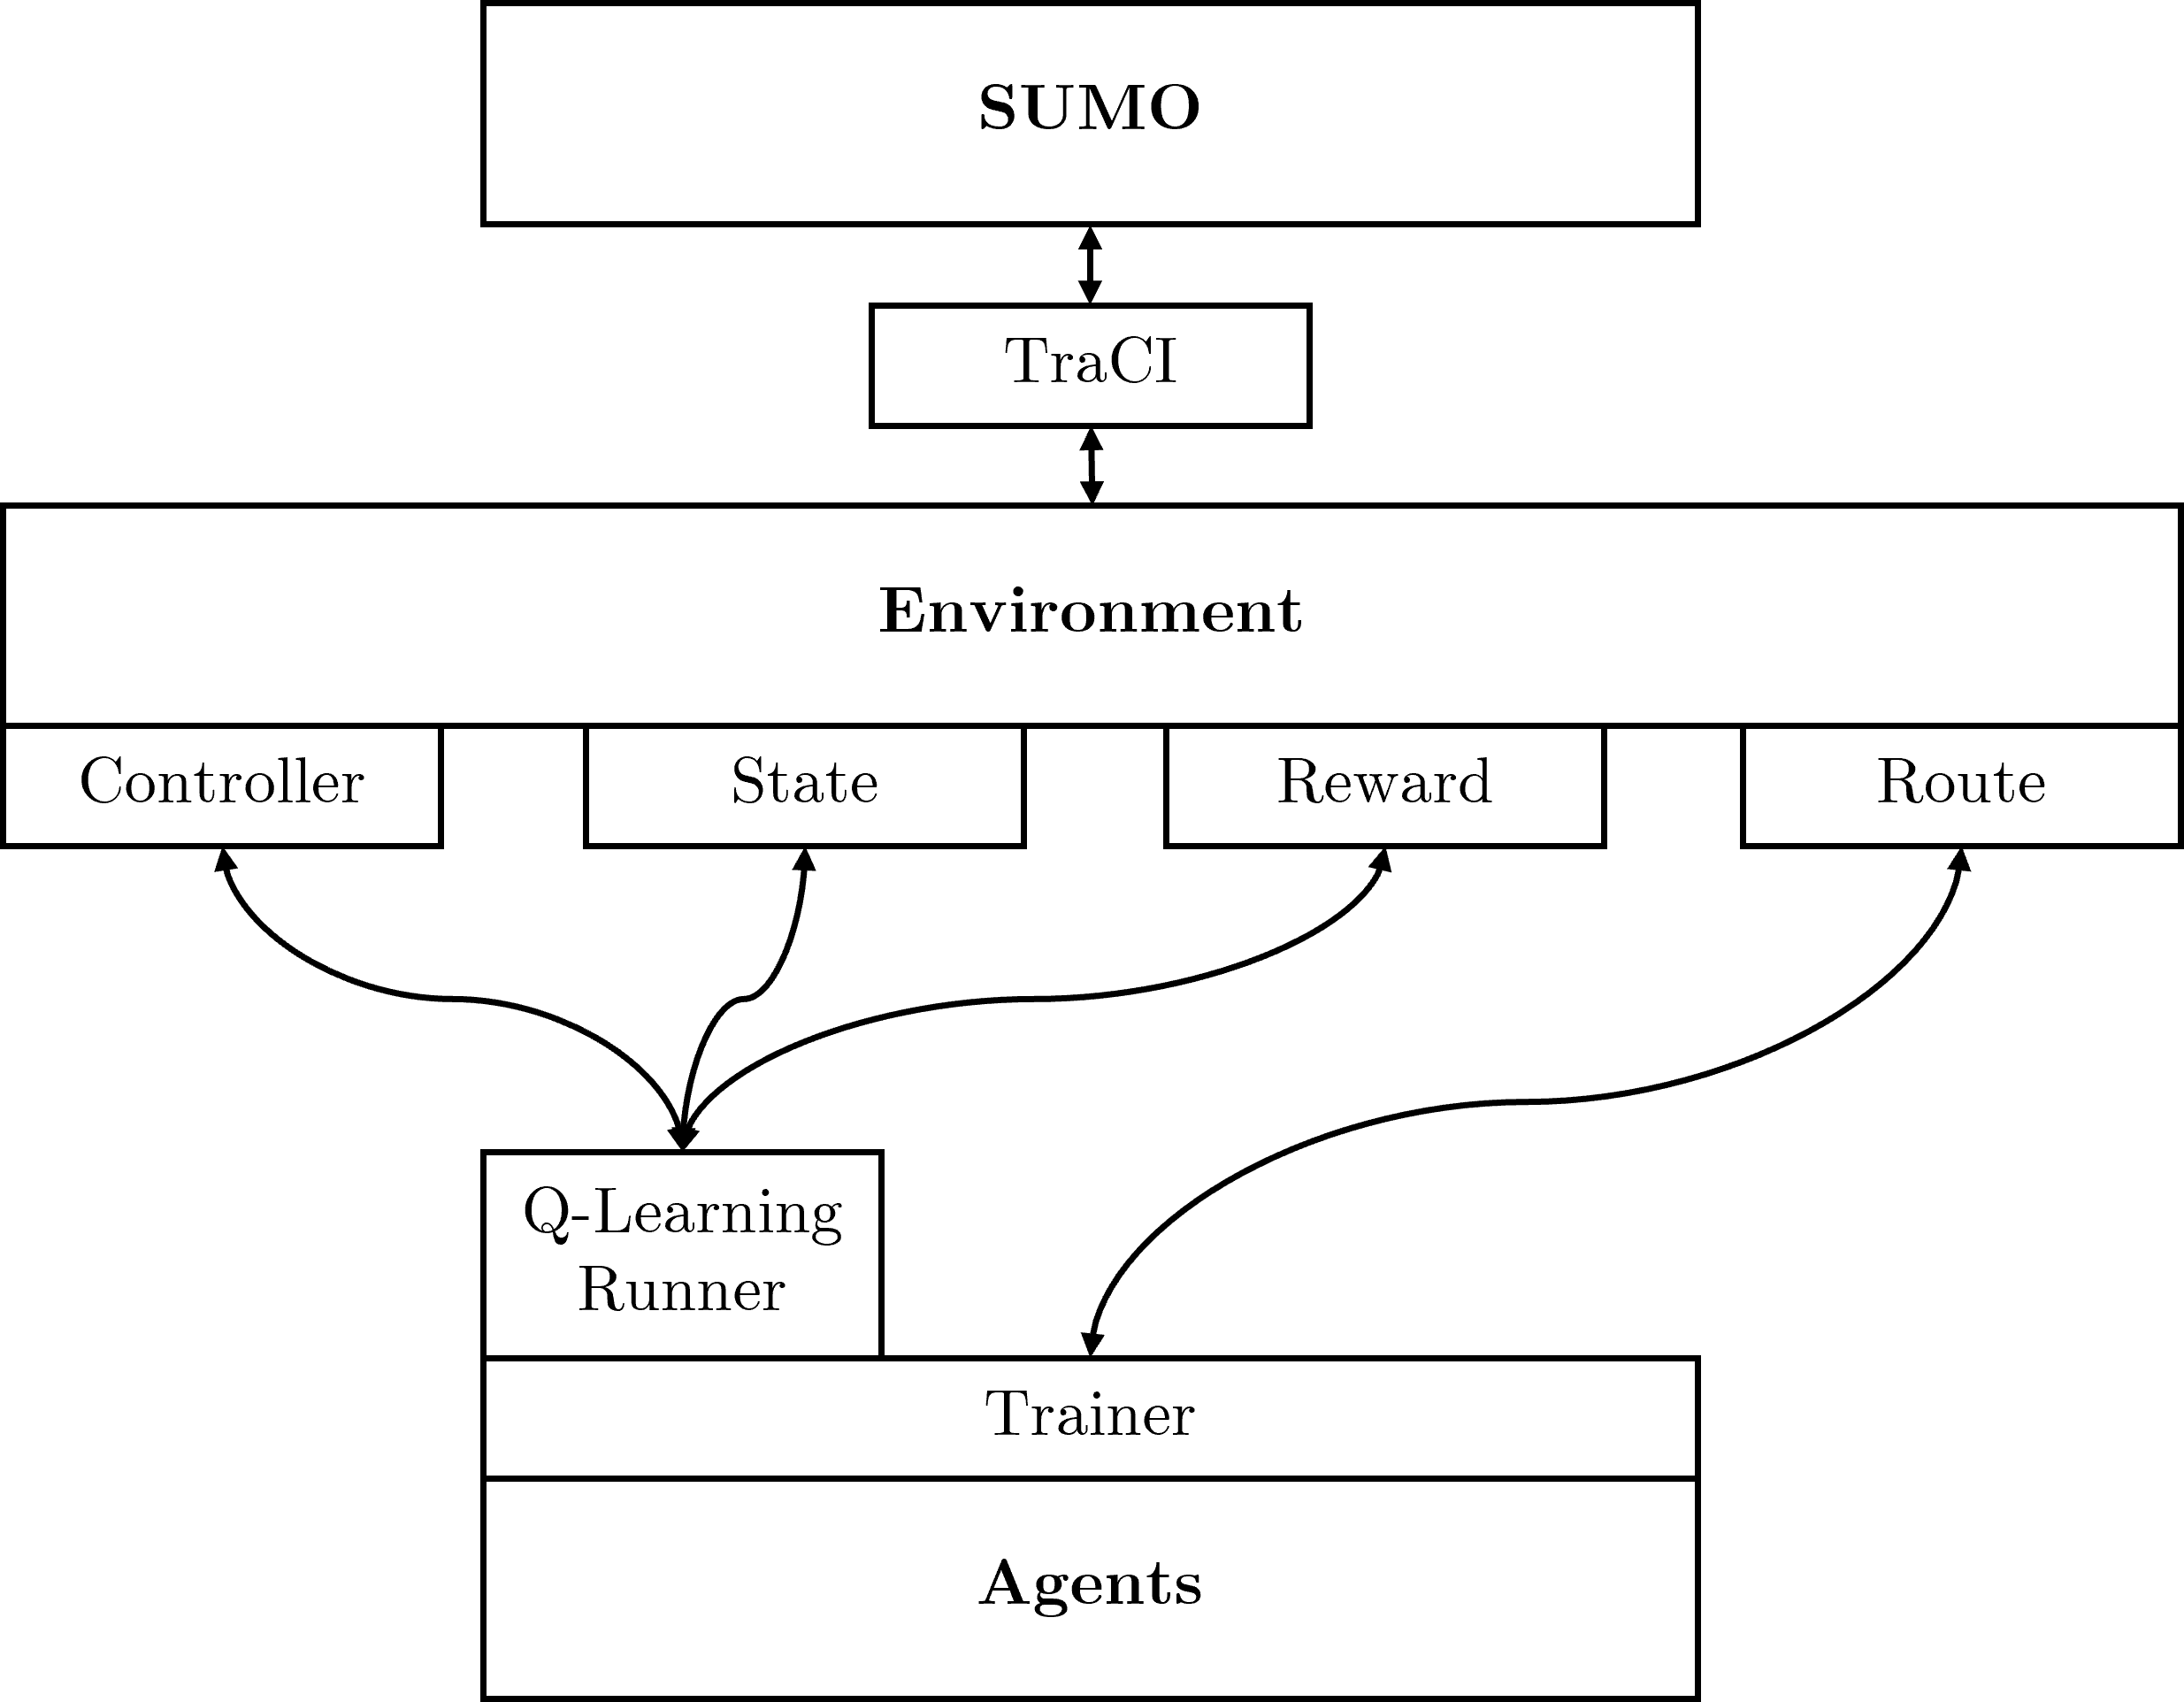
\includegraphics[width=0.64\textwidth]{images/implementation_demo.png}
    \caption{Library interactions overview.}
    \label{fig:implementation_demo}
\end{figure}

\section{Results}

\subsection{System Requirements}

The fixed-time control and Q-learning algorithms were implemented from scratch using Python, its standard library, and the \texttt{numpy} module. As stated previously, we rely on SUMO tooling and TraCI for creating and running the simulated traffic environment itself.

All code was developed and run locally, fortunately on performant hardware comparable to that which may be found in modern computer labs at a university. It was important to have easy, unrestricted access to diagnose and fix issues as soon as possible, and to train continuously for long hours, over multiple days in some cases.

\begin{table}[H]
  \centering
  \begin{tabular}{l|l}
    \textbf{Component} & \textbf{Specification} \\
    \hline
    CPU & Intel i5-13600K (3.50\,GHz, 14 cores) \\
    GPU & NVIDIA GeForce RTX 4070 Ti (12\,GB GDDR6X) \\
    RAM & 32\,GB DDR5 (6000\,MHz) \\
    Storage & 2\,TB PCIe 4.0 NVMe SSD \\
  \end{tabular}
  \caption{Local desktop machine specifications.}
  \label{fig:machine_specifications}
\end{table}

\subsection{Training} \label{q_learning_training}

We will train our agent, equipped with the Q-learning algorithm, inside the demo network using the 1000 traffic routes previously generated (each following the baseline traffic parameters). Each training episode -- or epoch -- has a duration of 3600 steps and corresponds to one of the routes. That is, at the start of each episode, a new route is set, before the agent trains for the specified number of steps. Once finished, the next episode begins.

\begin{figure}[H]
  \centering
  \begin{tikzpicture}
  \begin{axis}[
      width=14cm,
      height=8cm,
      xlabel={Epoch},
      ylabel={Reward},
      title={Demo network reward per epoch},
      grid=both,
      legend pos=south west
  ]

  \addplot[
      blue,
      mark=none
  ] table[
      x expr=\coordindex+1,
      y index=0
  ] {data/demo_train_ft_cleaned.txt};
  \addlegendentry{Fixed-time control}

  \addplot[
      orange,
      mark=none
  ] table[
      x expr=\coordindex+1,
      y index=0
  ] {data/demo_train_ql_c0.txt};
  \addlegendentry{Q-learning}

  \end{axis}
  \end{tikzpicture}
  \caption{Reward per training route in the demo environment.}
  \label{fig:q_learning_demo_train}
\end{figure}

Uh oh, it looks like something has gone terribly wrong! Figure~\ref{fig:q_learning_demo_train}\footnotemark\footnotetext{The figure data has been cleaned -- i.e.\ extreme outliers removed and a moving average applied -- for the sake of clarity.} shows that our Q-learning agent has failed to learn an effective policy for controlling the TLS. Instead of improving over time, the rewards diverge significantly, reaching values as low as $-3\times10^5$ compared to the baseline performance of $\sim0$ units.

This behaviour is explained by the size of the state space. Recall our state tuple $S$, consisting of 15 parts. The first element encodes the current TLS phase which can take one of three values: 1, 4, or 7. The next 6 elements correspond to the vehicle detectors each with a count in the range 0--8 on average. The remaining 8 elements correspond to our pedestrian detectors each with a count in the range of 0--6 on average.  

This results in a combinatorially large number of possible states ($3\times9^6\times7^8\approx9\times10^{12}$) that must be explored and learned. The agent struggles to sufficiently visit and update all state-action pairs enough times such that a good optimal policy is reached within the training period.

\subsection{Evaluation}

To evaluate the robustness and generalisability of the agent, we evaluate its performance in a set of evaluation routes with varied, unforeseen traffic conditions. We generate a total of 20 routes per evaluation configuration, and then take the median value per set allowing us to disregard outliers where there may have been teleportation penalties.

The evaluation configurations are defined as multiplicative scalars applied to the baseline insertion densities for cars, bicycles, and pedestrians defined in Table~\ref{tab:insertion_density_comparison}, which was $100$, $100$, and $200$ per hr/km respectively.

\begin{table}[H]
  \centering
  \begin{tabular}{c l l l}
    \hline
    & \textbf{Configuration} & \textbf{Scale ($\times$)} & \textbf{Description} \\
    \hline
    \textbf{1} & Baseline & (1.0, 1.0, 1.0) & Identical to the training environment parameters. \\
    \textbf{2} & High Density & (1.5, 1.5, 1.5) & Uniformly increased traffic across all entity types. \\
    \textbf{3} & Low Density & (0.5, 0.5, 0.5) & Uniformly reduced traffic across all entity types. \\
    \textbf{4} & Vehicle-Heavy & (1.5, 1.5, 0.5) & Increased road users, with fewer pedestrians. \\
    \textbf{5} & Pedestrian-Heavy & (0.5, 0.5, 1.5) & Increased pedestrians, with fewer road users. \\
    \hline
  \end{tabular}
  \caption{Comparison of the 5 evaluation configurations.}
  \label{tab:evaluation_configs}
\end{table}

Where each tuple in the scale column corresponds to (\emph{car}, \emph{bicycle}, \emph{pedestrian}). For example (0.5, 1.0, 1.5) means the \texttt{--insertion-density} for cars should be 0.5$\times$ the relevant baseline insertion density (50 per hr/km), for bicycles it should be 1.0$\times$ (100 per hr/km), and for pedestrians it should be 1.5$\times$ (300 per hr/km).

All other parameters passed to the \texttt{randomTrips.py} script besides \texttt{--insertion-density} remains unchanged. After generating the $20\times5=100$ evaluation scenarios, and taking the median value for each of the 5 sets, we get the following comparison as expected.

\begin{figure}[H]
  \centering
  \begin{tikzpicture}
  \begin{axis}[
      width=14cm,
      height=8cm,
      xlabel={Evaluation},
      ylabel={Reward},
      title={Demo network reward per evaluation scenario},
      grid=both,
      legend style={at={(0.03,0.5)},anchor=west},
      xtick=data
  ]

  \addplot[
      blue,
      mark=none
  ] table[
      x expr=\coordindex+1,
      y index=0
  ] {data/demo_eval_ft.txt};
  \addlegendentry{Fixed-time control}

  \addplot[
      orange,
      mark=none
  ] table[
      x expr=\coordindex+1,
      y index=0
  ] {data/demo_eval_ql_c0.txt};
  \addlegendentry{Q-learning}

  \end{axis}
  \end{tikzpicture}
  \caption{Median reward for evaluation routes in the demo environment.}
  \label{fig:q_learning_demo_eval}
\end{figure}

For each of the evaluation scenarios, our agent performed categorically worse than the fixed-time control TLS. This motivates our next algorithm which will use neural networks trained from scratch to deal with the issue of large state space that has lead to Q-learning performing so poorly.

\section{Summary}

This chapter explored the background of reinforcement learning, the state and actions relevant to our agent, and the Markov Decision Process. We then detailed the Q-learning algorithm which our agent uses, as well as the libraries which were implemented to facilitate the training of our agents.

Finally, we trained the agent and evaluated its performance in different scenarios against the standard fixed-time control algorithm. We conclude that our agent has performed substantially worse due to the large state space in the traffic light system, motivating the development of a smarter algorithm to resolve this. 

\chapter{Deep Q-Learning} \label{chapter:deep_q_learning}

Tabular Q-learning struggles to learn an effective policy in environments with a large state space, so we will extend the algorithm to Deep Q-learning. Rather than having to explicitly explore and update the quality value for each state-action pair, a neural network will be trained to approximate values. We will then train and evaluate the new agent, before considering next steps.

\section{Deep Q-Network}

As demonstrated in the previous chapter, an agent equipped with Q-learning alone is not sufficient for our needs. In our case, the state representation for the single traffic light system yields about $9\times10^{12}$ possible configurations, making it infeasible to sufficiently explore and update the Q-table within a training period of $1000$ epochs.

Addressing this limitation, we train and utilise Deep Q-Networks (DQN). This replaces the tabular representation of the Q-function in Figure~\ref{arr:q_table_example} with a parameterised function \emph{approximator}. Specifically, the neural network is used to estimate the optimal quality function $Q^*$.

$$Q(s, a; \theta) \approx Q^*(s, a)$$

Where $\theta$ represents the parameters (weights and biases) of the neural network.

A neural network consists of interconnected layers of nodes -- or neurons -- that learn patterns from data. It is used to solve complex problems where traditional rule-based approaches falls short. By adjusting connections based on example data, they automatically identify features and make decisions without being explicitly programmed for every scenario.

The input layer of our DQN consists of $m$ nodes corresponding to the $m$-tuple state $s$. The output layer is a vector of quality values for each of the $n$ possible actions $a$:

$$Q(s,\cdot;\theta)=[Q(s,a_1),Q(s,a_2),...,Q(s,a_n)]$$

\begin{figure}[H]
    \centering
    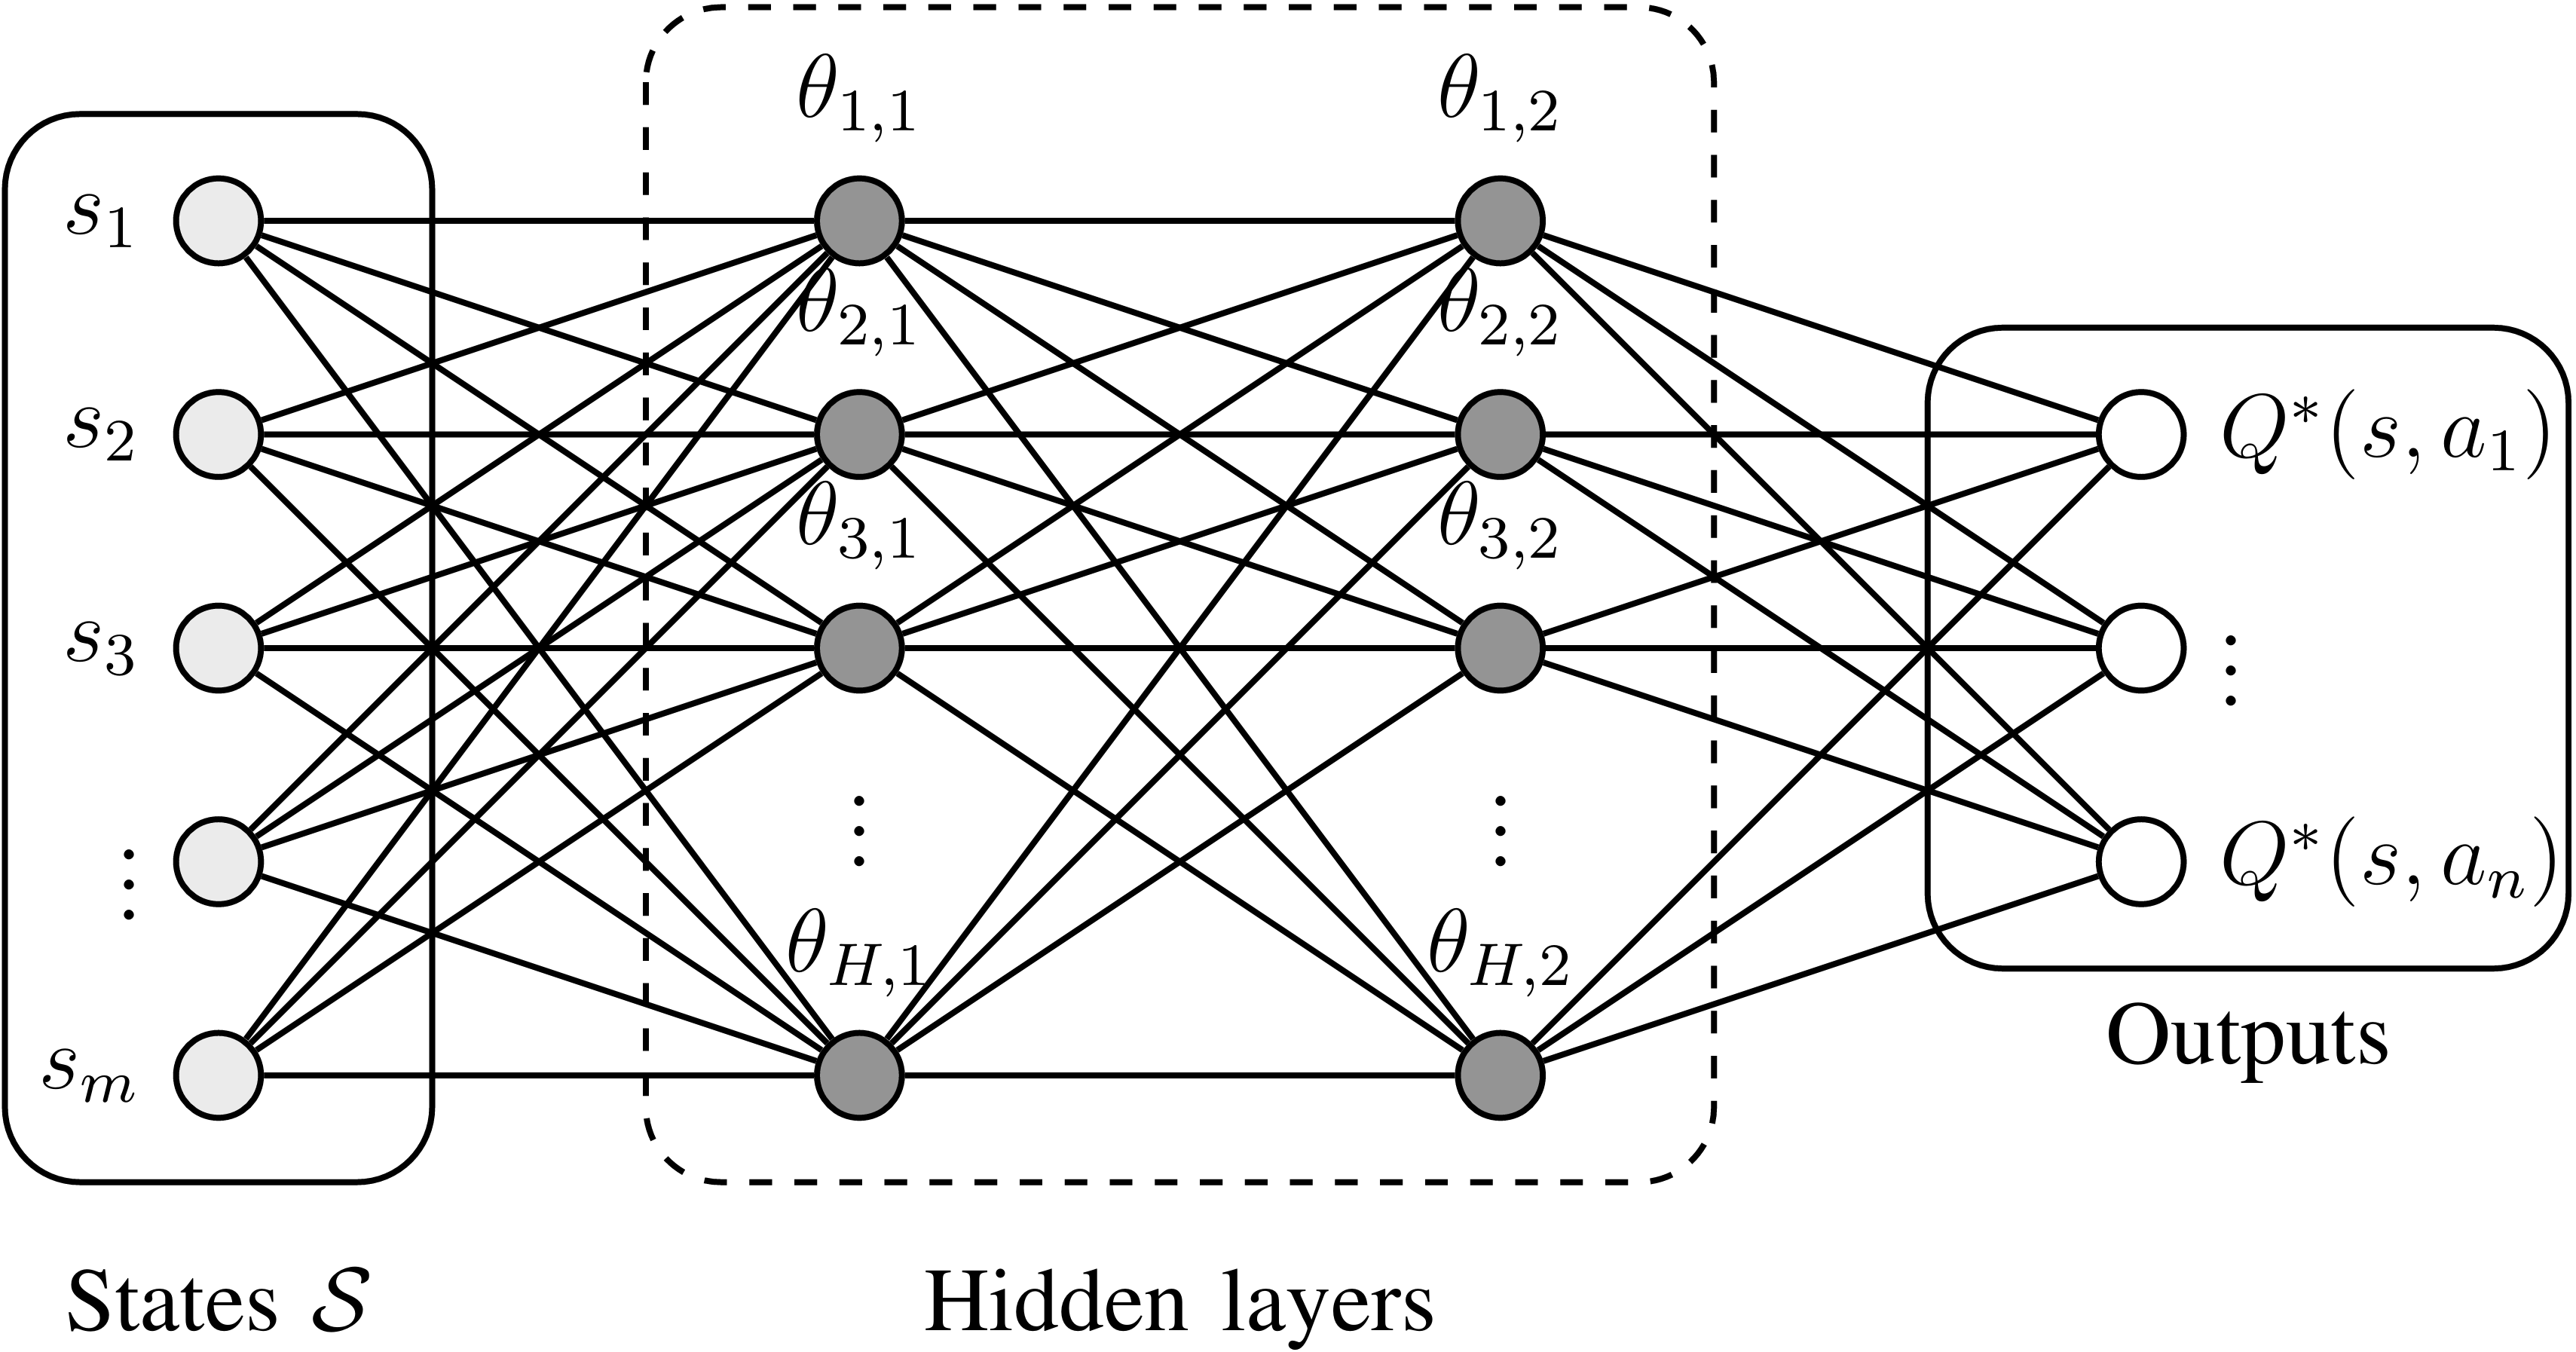
\includegraphics[width=0.75\textwidth]{images/neural_network.png}
    \caption{Example neural network with two hidden layers \cite{MismarChoiEvans2018}.}
    \label{fig:neural_network_example}
\end{figure}

The `best' action can be determined by choosing the action in the output vector with the highest quality value. By representing the Q-function this way, the agent can generalize its knowledge. If it encounters a never-before-seen state, the neural network can interpolate based on similar states it has already learned from.

\subsection{Experience Replay}

Reinforcement learning is known to be unstable or even to diverge when a neural network is used to represent the Q function, stemming from the correlations present in a sequence of observations \cite{SLi2023}. Training data samples are not independent -- the state at time $t+1$ is dependent on the state at time $t$.

To mitigate this temporal correlation, we introduce a mechanism called \emph{experience replay}. As the agent explores the environment, it stores its experiences in a replay memory buffer $D$. Each experience $e_t$ is stored as a tuple:

$$e_t=(s_t,a_t,R_t,s_{t+1},\delta_t,d_t)$$

Where $s$ is the state, $a$ is the action, $R$ is the reward, $\delta$ (`done') is a boolean flag to say if the action was the final action, and $d$ is the duration of the action (included since we are using a Semi-Markov Decision Process).

During training, instead of training on the most recent experience as with before, the agent samples a randomised batch of experiences from $D$. This ensures the neural network updates using a diverse set of uncorrelated transition, leading to more stable learning.

\subsection{Target Network}

In tabular Q-learning, the quality value was updated toward a target value calculated using the maximum estimated quality value of the next state. In a neural network, using the same network weights $\theta$ to calculate both the predicted quality value and the target quality value may lead to instability, as the target constantly shifts during every training step -- recall that it generalises rather than having distinct isolated Q-table entries.

Therefore our DQN employs a \emph{target network}. This is a second neural network with an identical architecture to the main \emph{policy network}, but with its own set of weights $\theta^-$ which is a delayed copy of the main network, used to compute the target quality value during training.

$$\theta^- \leftarrow \theta$$

The loss function $L$ for the policy neural network which we aim to minimise is the Mean Squared Error (MSE) between our current prediction and the target network's quality value $y$:

$$y=R + \gamma^d \max_{a'} Q(s', a'; \theta^-)$$

$$L(\theta) = \mathbb{E}\left[\left(y - Q(s, a; \theta)\right)^2\right]$$

The weights $\theta^-$ are updated only periodically to $\theta$, kept frozen to provide a stable target -- unlike the constantly changing main policy network.

\subsection{Algorithm}

\begin{algorithm}[H]
  \caption{Deep Q-Learning}
  \begin{algorithmic}[1]
  \State Initialise replay buffer $D$
  \State Initialise policy DQN with weights $\theta$, an optimiser, and learning rate $\alpha$
  \State Initialise target network with weights $\theta^- \leftarrow \theta$
  \For{each episode}
    \State Observe initial state $s$
    \For{each step in episode}
      \State Choose action $a$ using $\epsilon$-greedy policy
      \State Execute action $a$
      \State Observe reward $R$, next state $s'$, and duration $d$
      \State Store $(s,a,R,s',\delta,d)$ in buffer $D$
      \State Sample random batch of size $b$ from $D$
      \For{each sample $(s_i,a_i,R_i,s'_i,\delta_i,d_i)$}
        \State $y_i \leftarrow R_i + \gamma^{d_i} \underset{a'}\max Q(s'_i,a';\theta^-)$
      \EndFor
      \State Perform gradient descent on $L(\theta) = \frac{1}{b} \sum_{i=1}^{b} \left(y_i - Q(s_i, a_i; \theta)\right)^2$
      \State Update state $s \leftarrow s'$
      \State Periodically update $\theta^- \leftarrow \theta$ every $T$ steps
    \EndFor
  \EndFor
  \end{algorithmic}
\end{algorithm}

The overall algorithm follows a very similar structure to Tabular Q-Learning. We begin with setting up the replay buffer $D$ -- the `memory' -- and the two neural networks: the main policy DQN and the target DQN. A learning rate $\alpha$ and optimiser is not set for the latter since it is a target only to be used in evaluation mode.

The learning rate $\alpha$ controls the magnitude that the policy network updates its weights based on the gradient in line 14, whereas the optimiser is an algorithm which determines how the model updates its weights. $\alpha=0.0005$ was chosen alongside the \texttt{Adam} optimiser since they are the de facto standard for neural networks.

The gradient descent (i.e.\ the algorithm used to minimise the loss function) is performed on the average MSE loss for the $b$ samples in the batch taken from $D$.

$$L(\theta) = \frac{1}{b} \sum_{i=1}^{b} \left(y_i - Q(s_i, a_i; \theta)\right)^2$$

The size of the buffer $D$ was set to $2^{14}=16\,384$ and the batch size $b$ to $64$. The size of $D$ was chosen such it could store a wide range of experiences but not so large that we introduce duplicate data, or keep data that is now redundant. Whilst there isn't an agreed upon universal batch size in DQN literature, $64$ was chosen since it was small enough that updates were quick, but large enough that there was learning stability.

The target network is set to update every $T=72\,000$ steps (or 20 epochs). Delaying the target network update stabilises training by keeping the target quality values fixed for many steps. However, it is important to not set it too high lest the target becomes severely outdated.

\subsection{Implementation}

The overall system design remains unchanged from the previous chapters. In the same \texttt{Agents} library, we create a new \texttt{DeepQLearning} class that implements the abstract \texttt{Runner} class, as well two subordinate classes: \texttt{ReplayBuffer} for experience replay, and \texttt{DQN} for the neural networks themselves. fortunately, the code was designed such that adding new algorithms for our agent to use would not require extensive remodelling of the existing codebase.

\begin{figure}[H]
    \centering
    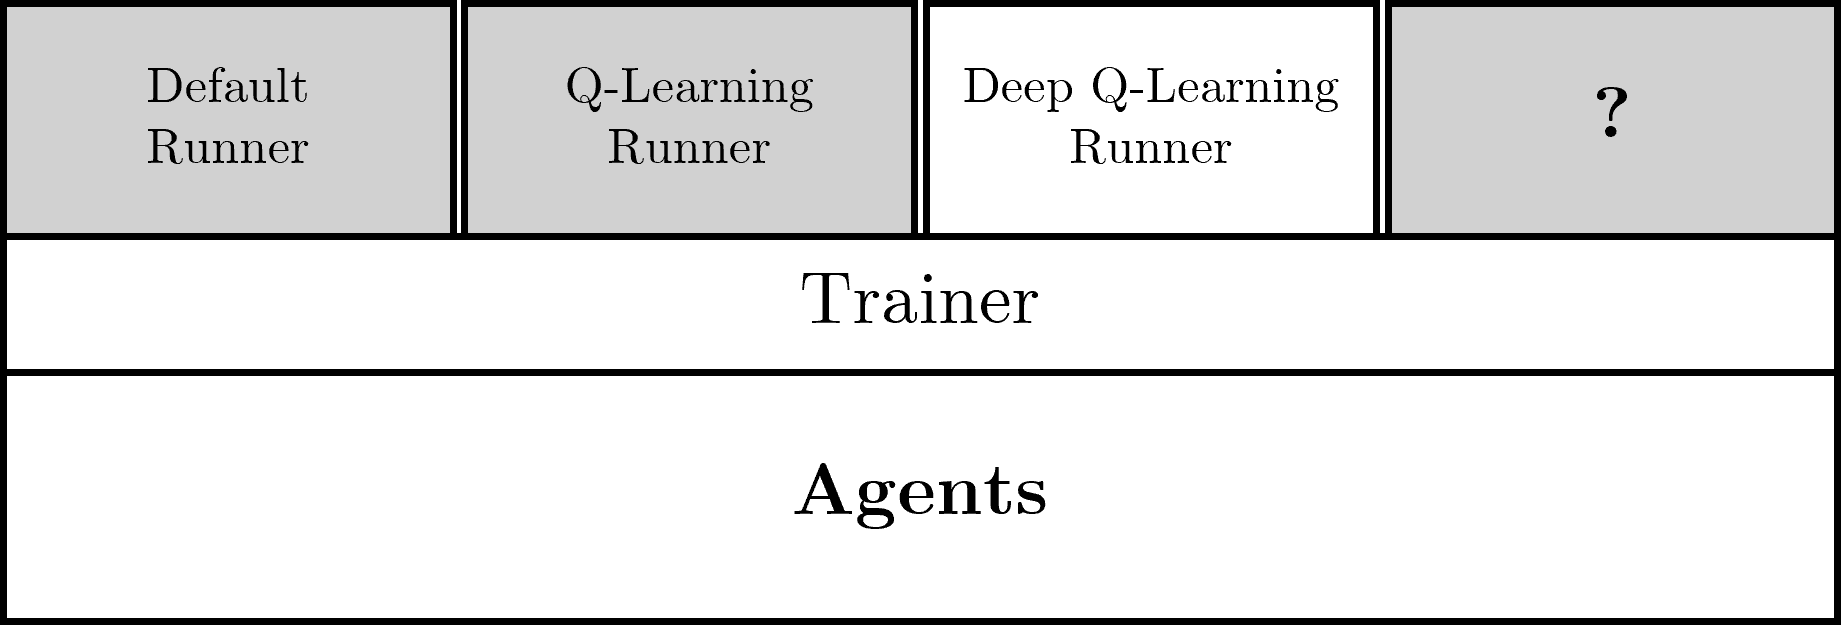
\includegraphics[width=0.64\textwidth]{images/implementation_crossing.png}
    \caption{Updated Agents library overview.}
    \label{fig:implementation_crossing}
\end{figure}

The DQN architecture varies based on the state tuple size and available actions for a TLS. For example, the TLS in the demo network will have an input layer of 15 nodes since the state tuple has 15 elements, and the output layer will have 3 nodes since we defined 3 actions. We choose two intermediary hidden layers of 64 nodes each for no particular reason besides it being a simple architecture to train.

\section{Crossing Network}

Before we train and evaluate the Deep Q-learning algorithm, we will create a new environment for us to test the agent in in addition to the demo network. Our new network -- `crossing network' -- will be a trimmed down version consisting of the single zebra crossing in \emph{Torrington Place} shown in OpenStreetMap. The netedit network editor was used to ensure the positioning of the crossings\footnotemark\footnotetext{\emph{Jaywalking} is strictly not allowed by default in SUMO.} were accurate.

\begin{figure}[H]
    \centering
    \begin{subfigure}{0.48\textwidth}
        \centering
        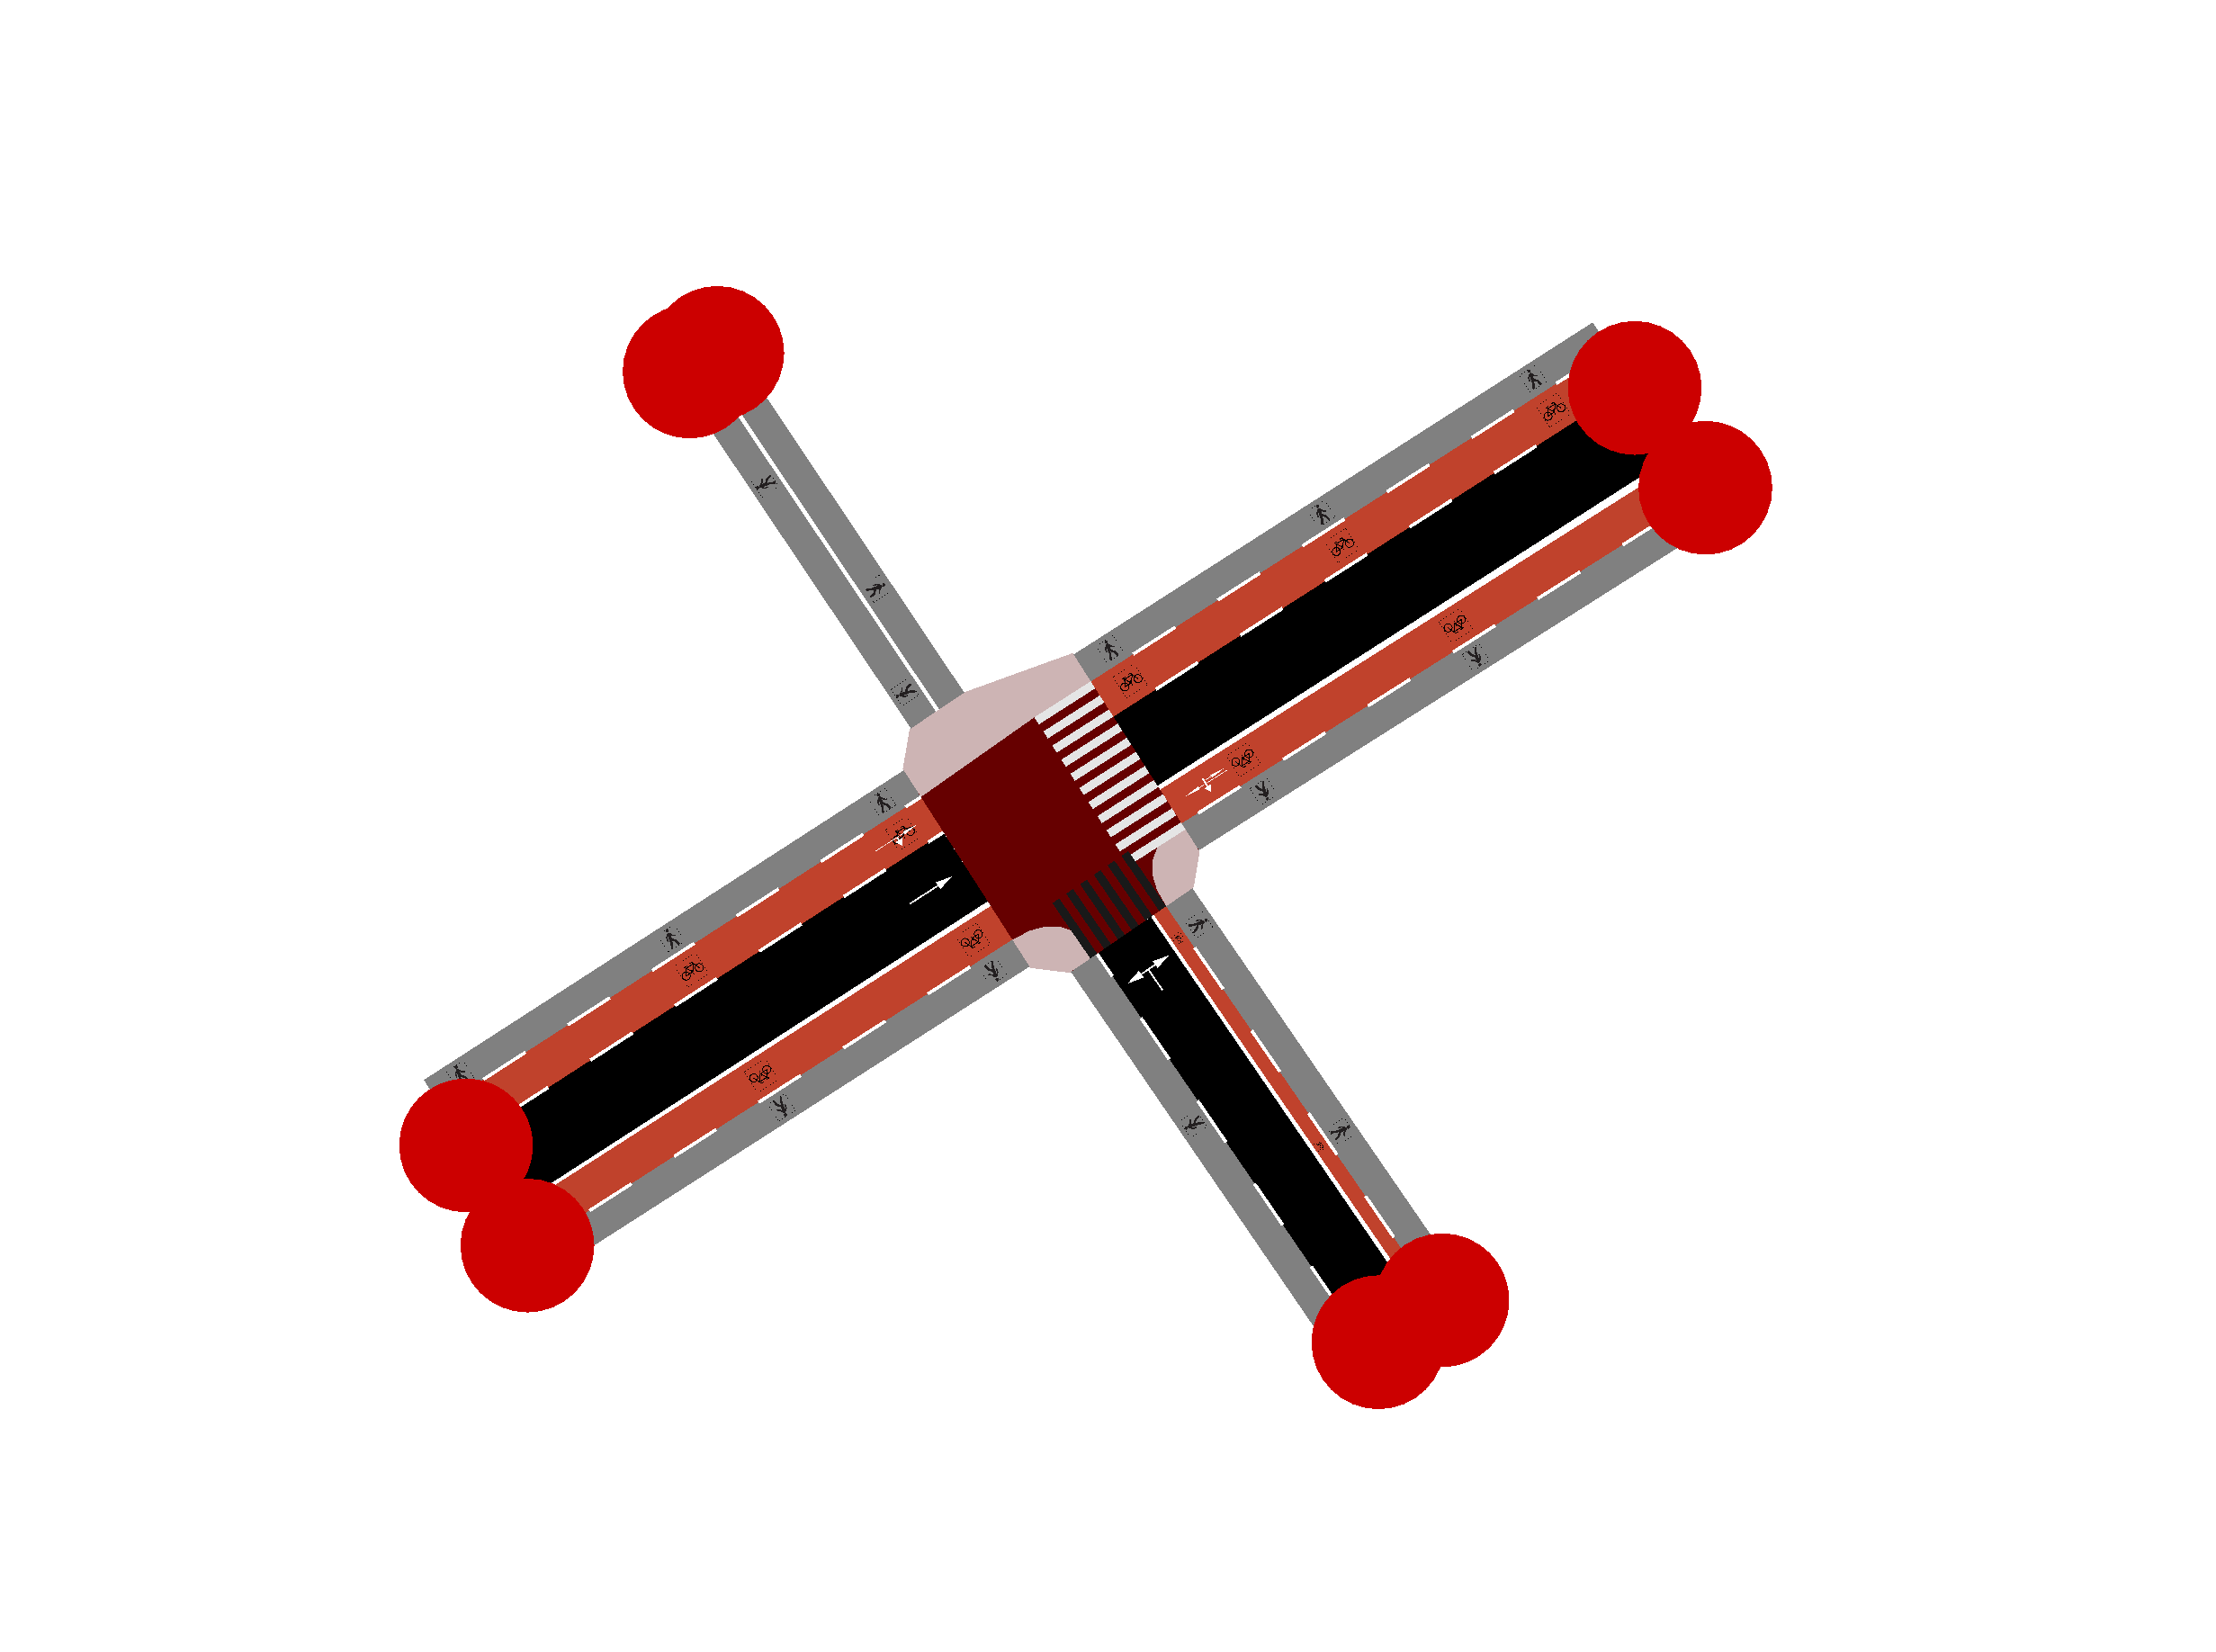
\includegraphics[width=\textwidth]{images/netedit_crossing.png}
        \caption{Road network in netedit.}
        \label{fig:netedit_crossing}
    \end{subfigure}
    \hfill
    \begin{subfigure}{0.48\textwidth}
        \centering
        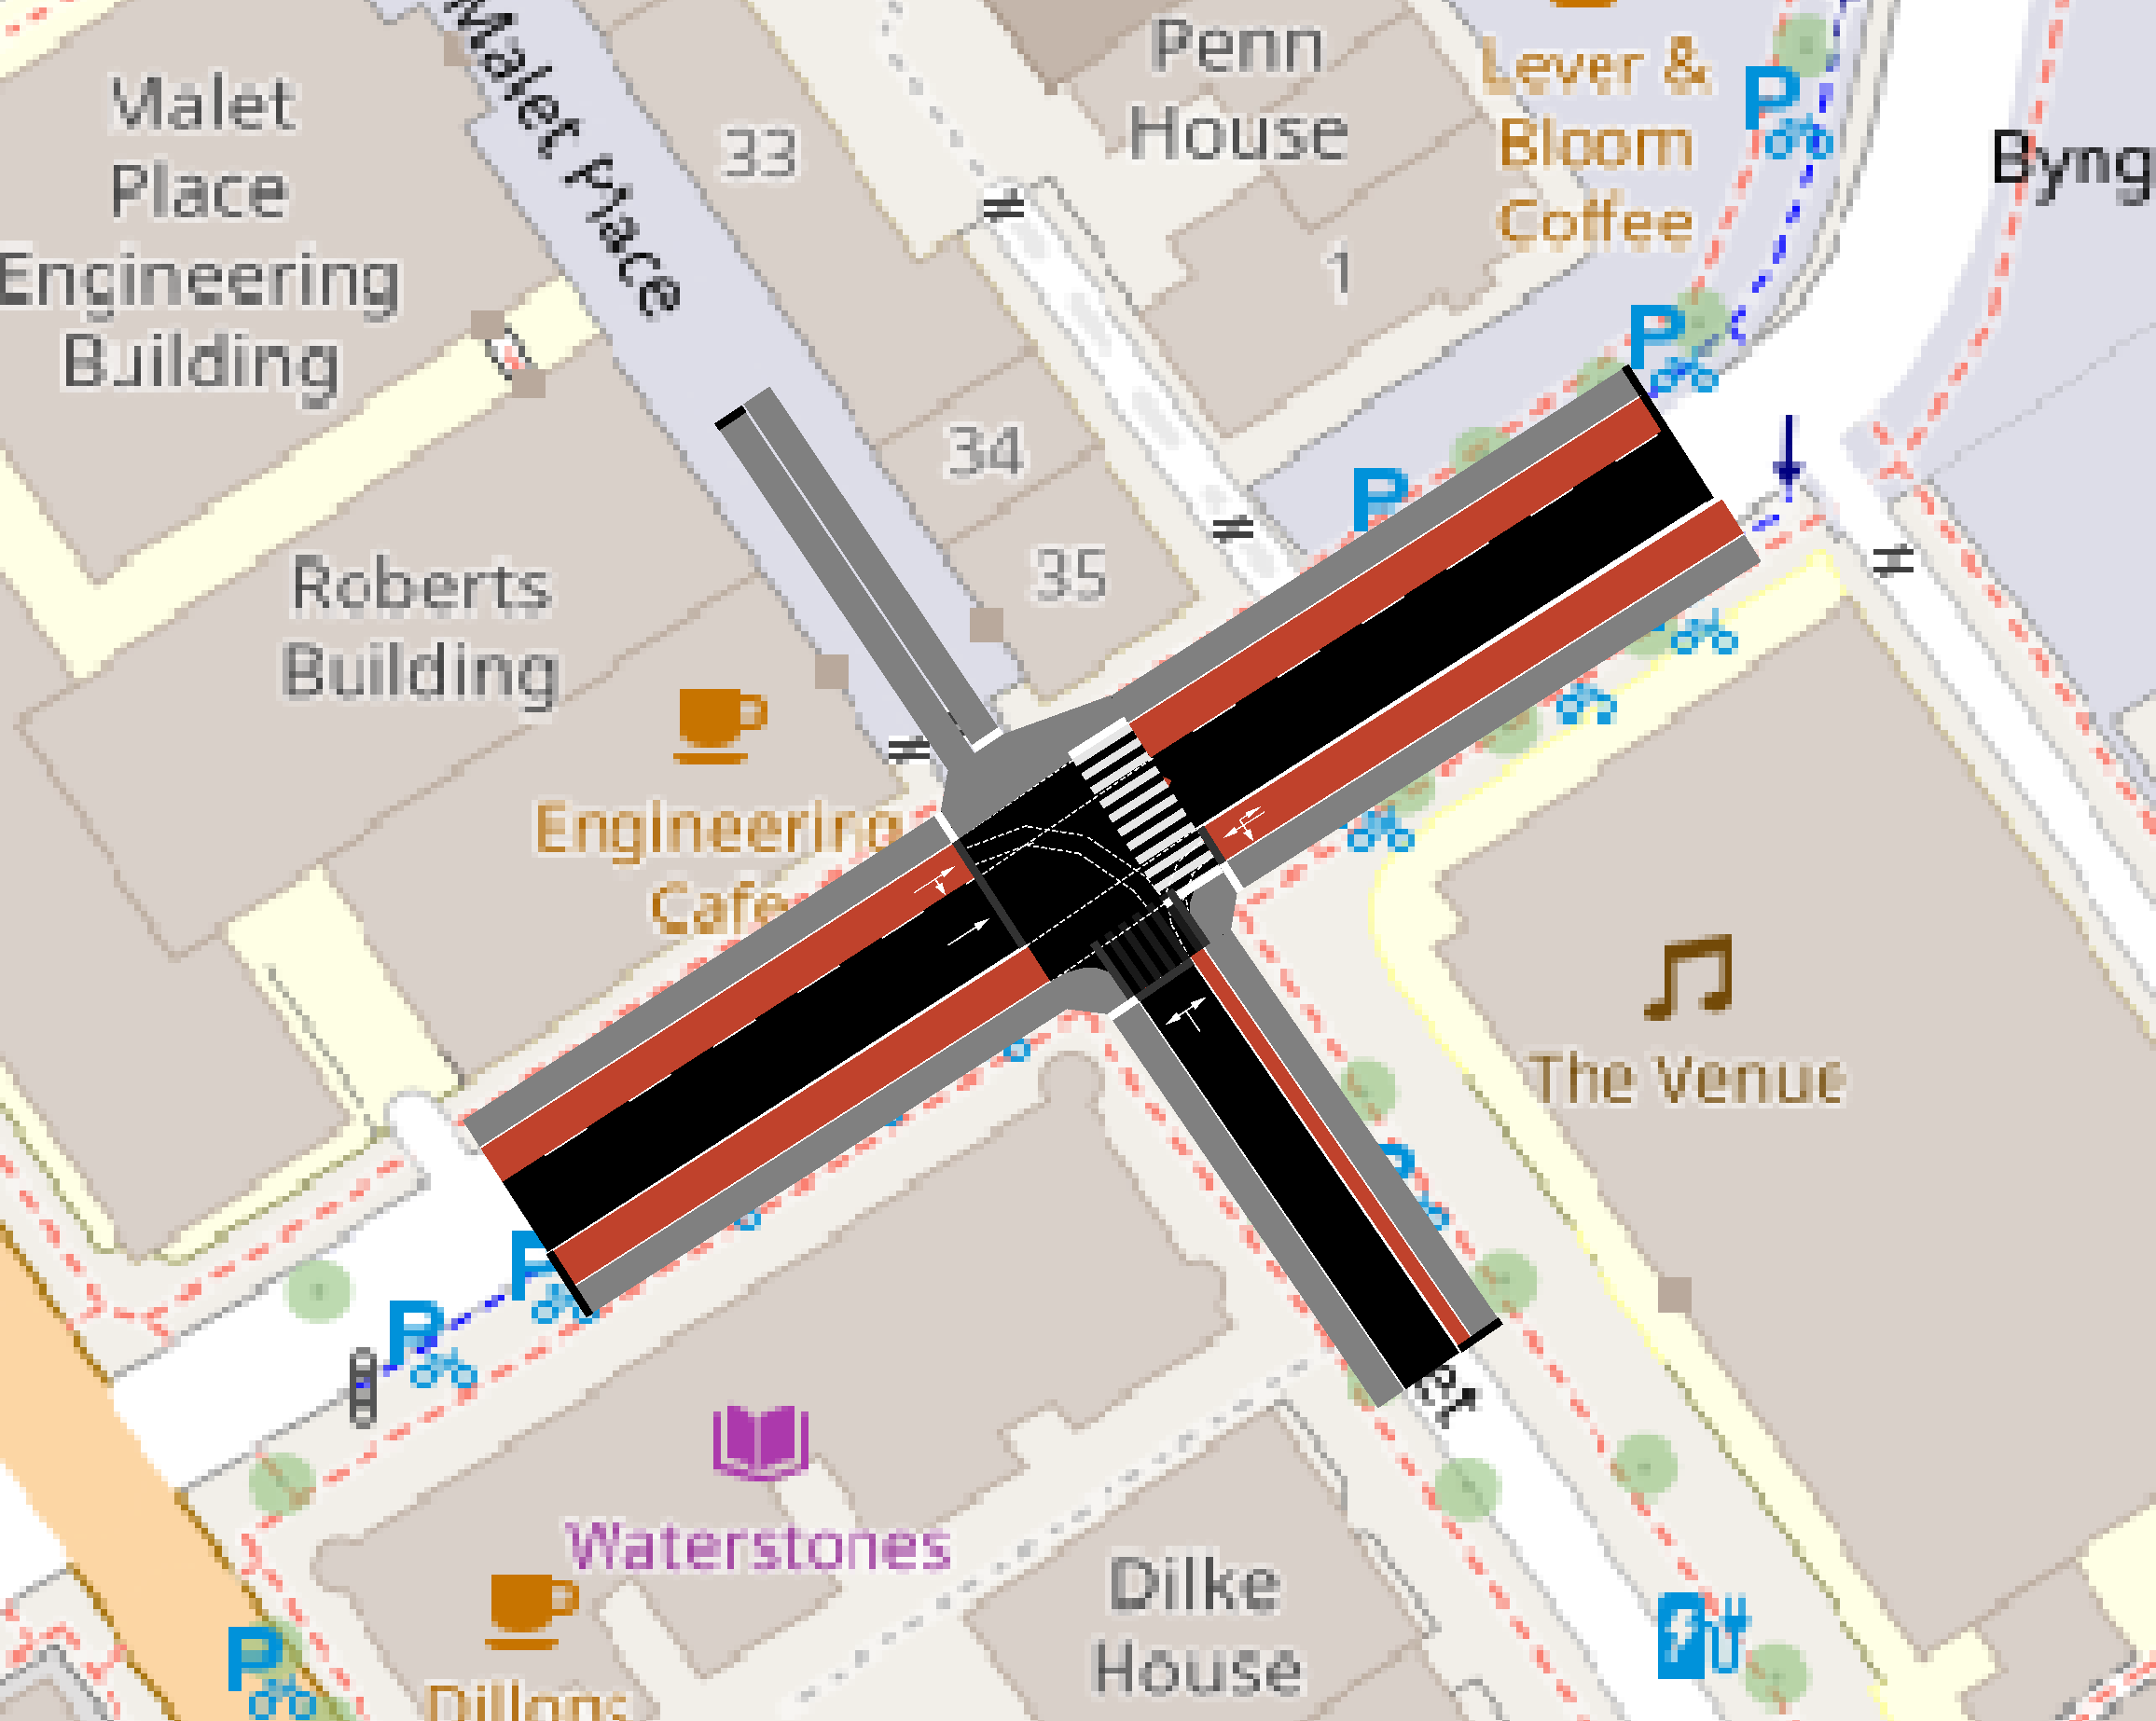
\includegraphics[width=\textwidth]{images/sumo_crossing.png}
        \caption{Simulation view in SUMO.}
        \label{fig:sumo_crossing}
    \end{subfigure}
    \caption{Crossing simulation environment.}
    \label{fig:crossing_simulation}
\end{figure}

As seen in Figure~\ref{fig:sumo_crossing}, the scope is substantially smaller than before. The motivation behind this decision is twofold: firstly, we want to evaluate our agent in diverse settings, and secondly it would be interesting to observe how our agent fares in comparison to a zebra crossing -- not just traditional fixed-time control TLS.

Since this is a different traffic light system, the lane configurations and therefore number of detectors and state differs from before. We still use yellow-coloured induction loops placed on departure lanes, aqua-coloured lane area detectors placed on the approaches, and pseudo-detectors for the two pedestrian crossings.

\begin{figure}[H]
    \centering
    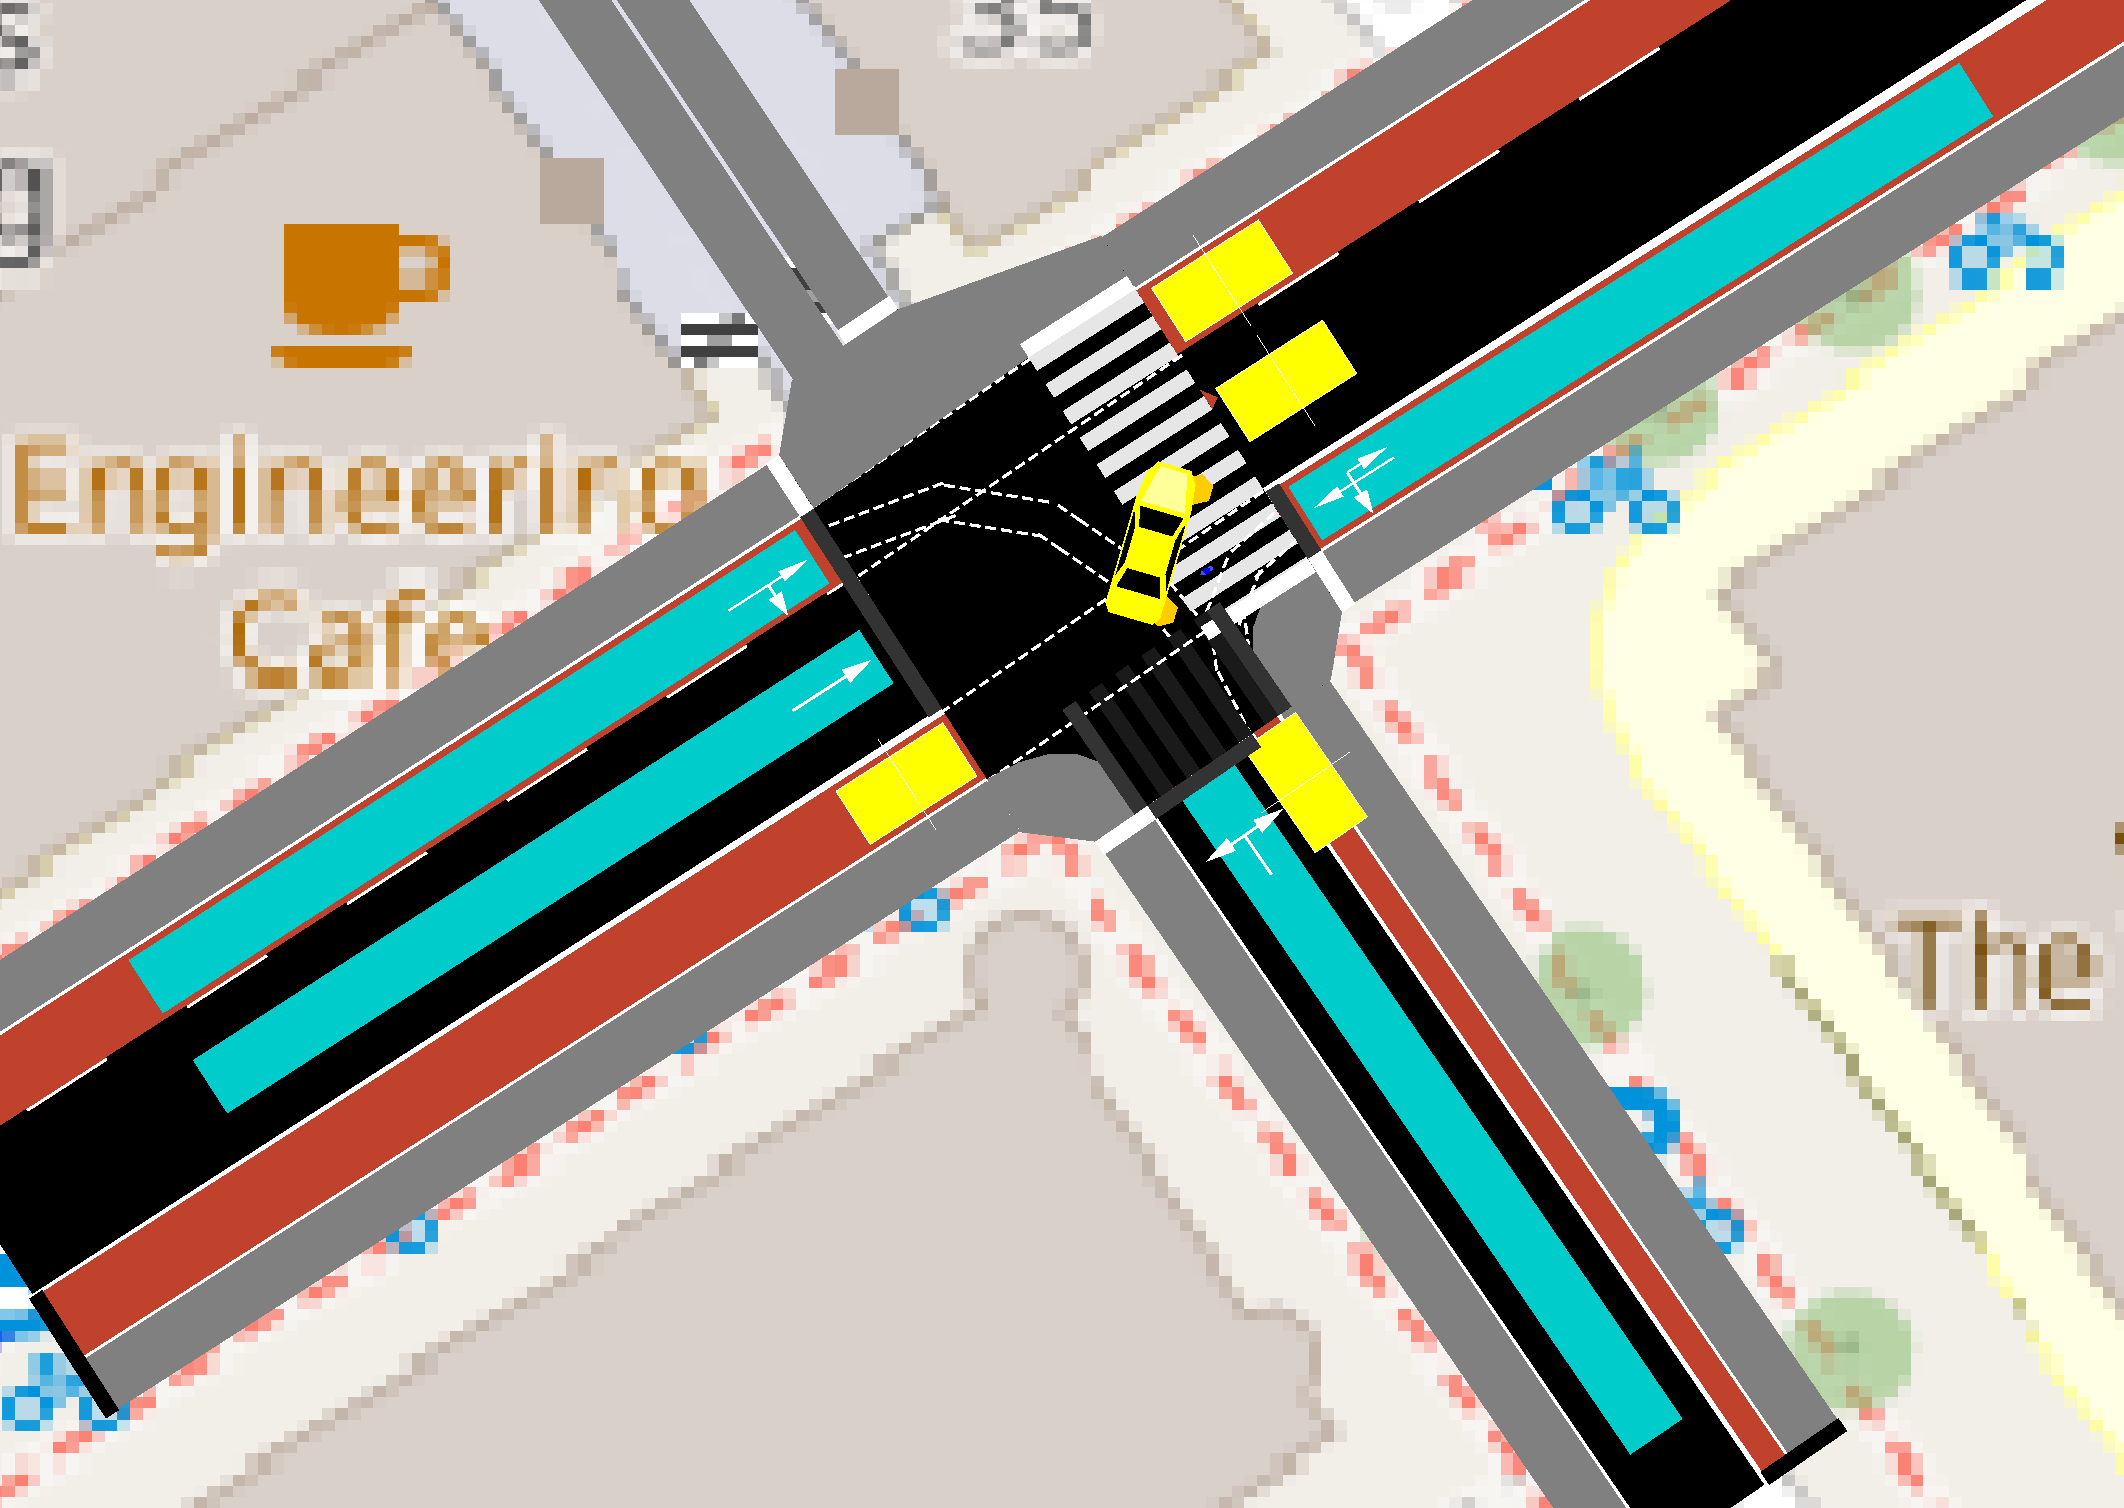
\includegraphics[width=0.48\textwidth]{images/zebra_crossing.png}
    \caption{Detectors in the crossing network.}
    \label{fig:detectors_crossing}
\end{figure}

Evidently a zebra crossing is not something that can be controlled by our agent. So to evaluate the performance of our agent compared to a standard zebra crossing, we will create an alternative network which is the exact same except there is instead a traffic light system that controls the lane approaches and crossings, which our agent \emph{can} control. The state tuple consists of 9 elements using the general formula defined in formula \eqref{state_formula}, annotated below.

\begin{figure}[H]
    \centering
    
\includegraphics[width=0.64\textwidth]{images/state_crossing.png}
    \caption{Annotated state in the crossing network (with a traffic light system).}
    \label{fig:state_crossing}
\end{figure}

The action space -- 3 actions -- will remain the same as before. We have maintained a notion of \emph{northbound}/\emph{southbound} and \emph{eastbound}/\emph{westbound} lane approaches in our crossing network, therefore the same exact traffic light system phase structure defined in Table~\ref{tab:phase_structure}, as well as the agent actions defined in Table~\ref{tab:phase_actions}, can be reused. 

Fortunately the route generation parameters also remain exactly as before. Recalling the baseline traffic parameter definitions, we used the \texttt{--insertion-density} parameter to control how many cars, bicycles, and pedestrians there were. Since it is given in units of $per\ hr/km$, the total magnitude of traffic scales uniformly with the road network size (whilst maintaining traffic density).

\section{Results}

\subsection{System Requirements}

The Deep Q-learning algorithm was implemented from scratch using Python and the same libraries as before. In addition, we also now use the \texttt{PyTorch} module to build, train, and run the neural networks which we use, and it also comes with the \texttt{Adam} optimiser, MSE loss function, and utilities such as saving and loading models to and from disk.

Training was optimised by configuring \texttt{PyTorch} to offload the tensor operations and neural network backpropagation to the NVIDIA GeForce RTX 4070 Ti GPU, utilising CUDA. It is important to note that the SUMO environment simulation does not support GPU acceleration, remaining CPU-bound.

\subsection{Training}

There are two distinct agents we train, both utilising the deep Q-learning algorithm. One will be trained for the TLS in the demo network, and the other will be trained for the TLS in the crossing network. Both will be trained using 1000 traffic routes which follow the baseline traffic parameters. Each training episode has a duration of 3600 steps as with the Q-learning agent previously.

\begin{figure}[H]
  \centering
  \begin{tikzpicture}
  \begin{axis}[
      width=14cm,
      height=8cm,
      xlabel={Epoch},
      ylabel={Reward},
      title={Demo network reward per epoch},
      grid=both,
      legend pos=south east
  ]

  \addplot[
      blue,
      mark=none
  ] table[
      x expr=\coordindex+1,
      y index=0
  ] {data/demo_train_ft_cleaned.txt};
  \addlegendentry{Fixed-time control}

  \addplot[
      orange,
      mark=none
  ] table[
      x expr=\coordindex+1,
      y index=0
  ] {data/demo_train_dqn_c0.txt};
  \addlegendentry{Deep Q-learning}

  \end{axis}
  \end{tikzpicture}
  \caption{Reward per training route in the demo environment.}
  \label{fig:deep_q_learning_demo_train}
\end{figure}

Looking at the data in Figure~\ref{fig:deep_q_learning_demo_train}, we can see that our Deep Q-learning agent has successfully learned an effective policy for controlling the TLS. It steadily improves over time, before the rewards converge to around $\sim4\,000$ units. This confirms that the issue of state space size has been overcome.

\begin{figure}[H]
  \centering
  \begin{tikzpicture}
  \begin{axis}[
      width=14cm,
      height=8cm,
      xlabel={Epoch},
      ylabel={Reward},
      title={Crossing network reward per epoch},
      grid=both,
      legend pos=south east
  ]

  \addplot[
      green,
      mark=none
  ] table[
      x expr=\coordindex+1,
      y index=0
  ] {data/crossing_train_zebra.txt};
  \addlegendentry{Zebra}

  \addplot[
      blue,
      mark=none
  ] table[
      x expr=\coordindex+1,
      y index=0
  ] {data/crossing_train_ft.txt};
  \addlegendentry{Fixed-time control}

  \addplot[
      orange,
      mark=none
  ] table[
      x expr=\coordindex+1,
      y index=0
  ] {data/crossing_train_dqn_c0.txt};
  \addlegendentry{Deep Q-learning}

  \end{axis}
  \end{tikzpicture}
  \caption{Reward per training route in the crossing environment.}
  \label{fig:deep_q_learning_crossing_train}
\end{figure}

In Figure~\ref{fig:deep_q_learning_crossing_train}, the fixed-time control has an average reward of around $50$ units (the reward is normalised to the demo environment, \emph{not} crossing), compared to the zebra crossing which performs much better at around $900$ units. We observe that our deep Q-learning gets very close to the zebra crossing in terms of performance as it trains, but not quite there.

\subsection{Evaluation}

Now we evaluate both of the agents in their respective network using the same evaluation configurations defined in the previous chapter in Table~\ref{tab:evaluation_configs}. After generating the 100 evaluation scenarios, and taking the median values, we get the following results.

\begin{figure}[H]
  \centering
  \begin{tikzpicture}
  \begin{axis}[
      width=14cm,
      height=8cm,
      xlabel={Evaluation},
      ylabel={Reward},
      title={Demo network reward per evaluation scenario},
      grid=both,
      legend style={at={(0.03,0.5)},anchor=west},
      xtick=data
  ]

  \addplot[
      blue,
      mark=none
  ] table[
      x expr=\coordindex+1,
      y index=0
  ] {data/demo_eval_ft.txt};
  \addlegendentry{Fixed-time control}

  \addplot[
      orange,
      mark=none
  ] table[
      x expr=\coordindex+1,
      y index=0
  ] {data/demo_eval_dqn_c0.txt};
  \addlegendentry{Deep Q-learning}

  \end{axis}
  \end{tikzpicture}
  \caption{Median reward for evaluation routes in the demo environment.}
  \label{fig:deep_q_learning_demo_eval}
\end{figure}

For each of the evaluation scenarios, our Deep Q-learning agent performed better than the fixed-time control TLS, vindicating our efforts in building a reinforcement learning agent to control traffic lights.

\begin{figure}[H]
  \centering
  \begin{tikzpicture}
  \begin{axis}[
      width=14cm,
      height=8cm,
      xlabel={Evaluation},
      ylabel={Reward},
      title={Crossing network reward per evaluation scenario},
      grid=both,
      legend style={at={(0.97,0.97)},anchor=north east},
      xtick=data
  ]

  \addplot[
      green,
      mark=none
  ] table[
      x expr=\coordindex+1,
      y index=0
  ] {data/crossing_eval_zebra.txt};
  \addlegendentry{Zebra}

  \addplot[
      blue,
      mark=none
  ] table[
      x expr=\coordindex+1,
      y index=0
  ] {data/crossing_eval_ft.txt};
  \addlegendentry{Fixed-time control}

  \addplot[
      orange,
      mark=none
  ] table[
      x expr=\coordindex+1,
      y index=0
  ] {data/crossing_eval_dqn_c0.txt};
  \addlegendentry{Deep Q-learning}

  \end{axis}
  \end{tikzpicture}
  \caption{Median reward for evaluation routes in the crossing environment.}
  \label{fig:deep_q_learning_crossing_eval}
\end{figure}

For each scenario, the standard zebra crossing performs the best, followed closely by our Deep Q-learning agent, then finally the fixed-time control TLS which performs the worst by a significant margin. Taking these results at face value, it would be easy to conclude that zebra crossings are the definite right choice, and that traffic light systems -- especially one that is \emph{not} intelligent -- should not be used.

However, as mentioned in the problem statement, traffic lights were introduced to control flow for safety and better traffic regulation. Zebra crossings are about as efficient as you can get in cases where urban traffic is sparse, but they generally have less safety guarantees compared to a standard TLS. It relies on vehicle compliance and giving way to pedestrians, which vehicles may unfortunately not always adhere to -- particularly during periods of large pedestrian influx. Furthermore, they become significantly more dangerous when vehicles exceed $30$\ mph \cite{ActiveTravel25}.

The Deep Q-learning agent, though not as good in terms of raw performance, performs decently well whilst providing the innate safety features of a standard traffic light system which are explicitly designed to prevent vehicles and pedestrians from occupying the same road area at the same time.

\section{Summary}

This chapter explored the motivation for introducing Deep Q-learning in the first place, the theory behind how it works, a detailed description of the algorithm, and an implementation overview. In addition, we covered the creation of a new crossing network alongside the old demo network, enabling us to evaluate the performance of zebra crossings.

Finally, we trained the agent in the two distinct networks and evaluated its overall performance. We conclude that our agent performs significantly better than a standard fixed-time control traffic light system, but not quite as good as a zebra crossing in all five of the evaluation scenarios.

\chapter{Communicative Deep Q-Learning} \label{chapter:communicative_deep_q_learning}

We conclude our algorithms with an extension of Deep Q-learning that enables communication with other agents. Previously, our agents were confined to a single traffic light system without a way of knowing adjacent states, so we will develop a way for agents to exchange messages in a distributed manner via a communication bus. We will then train and evaluate the multi-agent system.

\section{Network Layer}

Although our single agent system performed well when equipped with Deep Q-learning, it was not able to accommodate interactions between multiple traffic light systems (TLS). Intuitively, adjacent traffic light junctions should be highly interdependent, since the decision made at one junction directly influences traffic conditions at neighbouring junctions.

To evaluate the benefit of agent communication, we first introduce a \emph{network layer} $N$ which enables multiple agents to operate their own TLS simultaneously in a given environment in the first place. This builds upon our previous Deep Q-learning implementation with SUMO which only enabled \emph{one} agent-controlled TLS in an environment even if there were multiple TLS.

$$
N_n=
\left\{
  \begin{array}{cc}
    Q(s_1, a_1; \theta_1) & (1)\\
    Q(s_2, a_2; \theta_2) & (2)\\
    \vdots & \vdots\\
    Q(s_n, a_n; \theta_n) & (n)\\
  \end{array}
\right.
$$

Where $n$ is the number of agent controlled traffic lights. As we can see, for each agent, there is a distinct state $s$, action $a$, and set of parameters (weights and biases) $\theta$. 

Note that the network layer simply enables multiple agents to operate simultaneously. Although we have listed the agents as using the Deep Q-learning algorithm $Q(s, a; \theta)$, they could as well use the standard Q-learning algorithm $Q(s, a)$, or just a basic fixed-time control algorithm.

\begin{figure}[H]
    \centering
    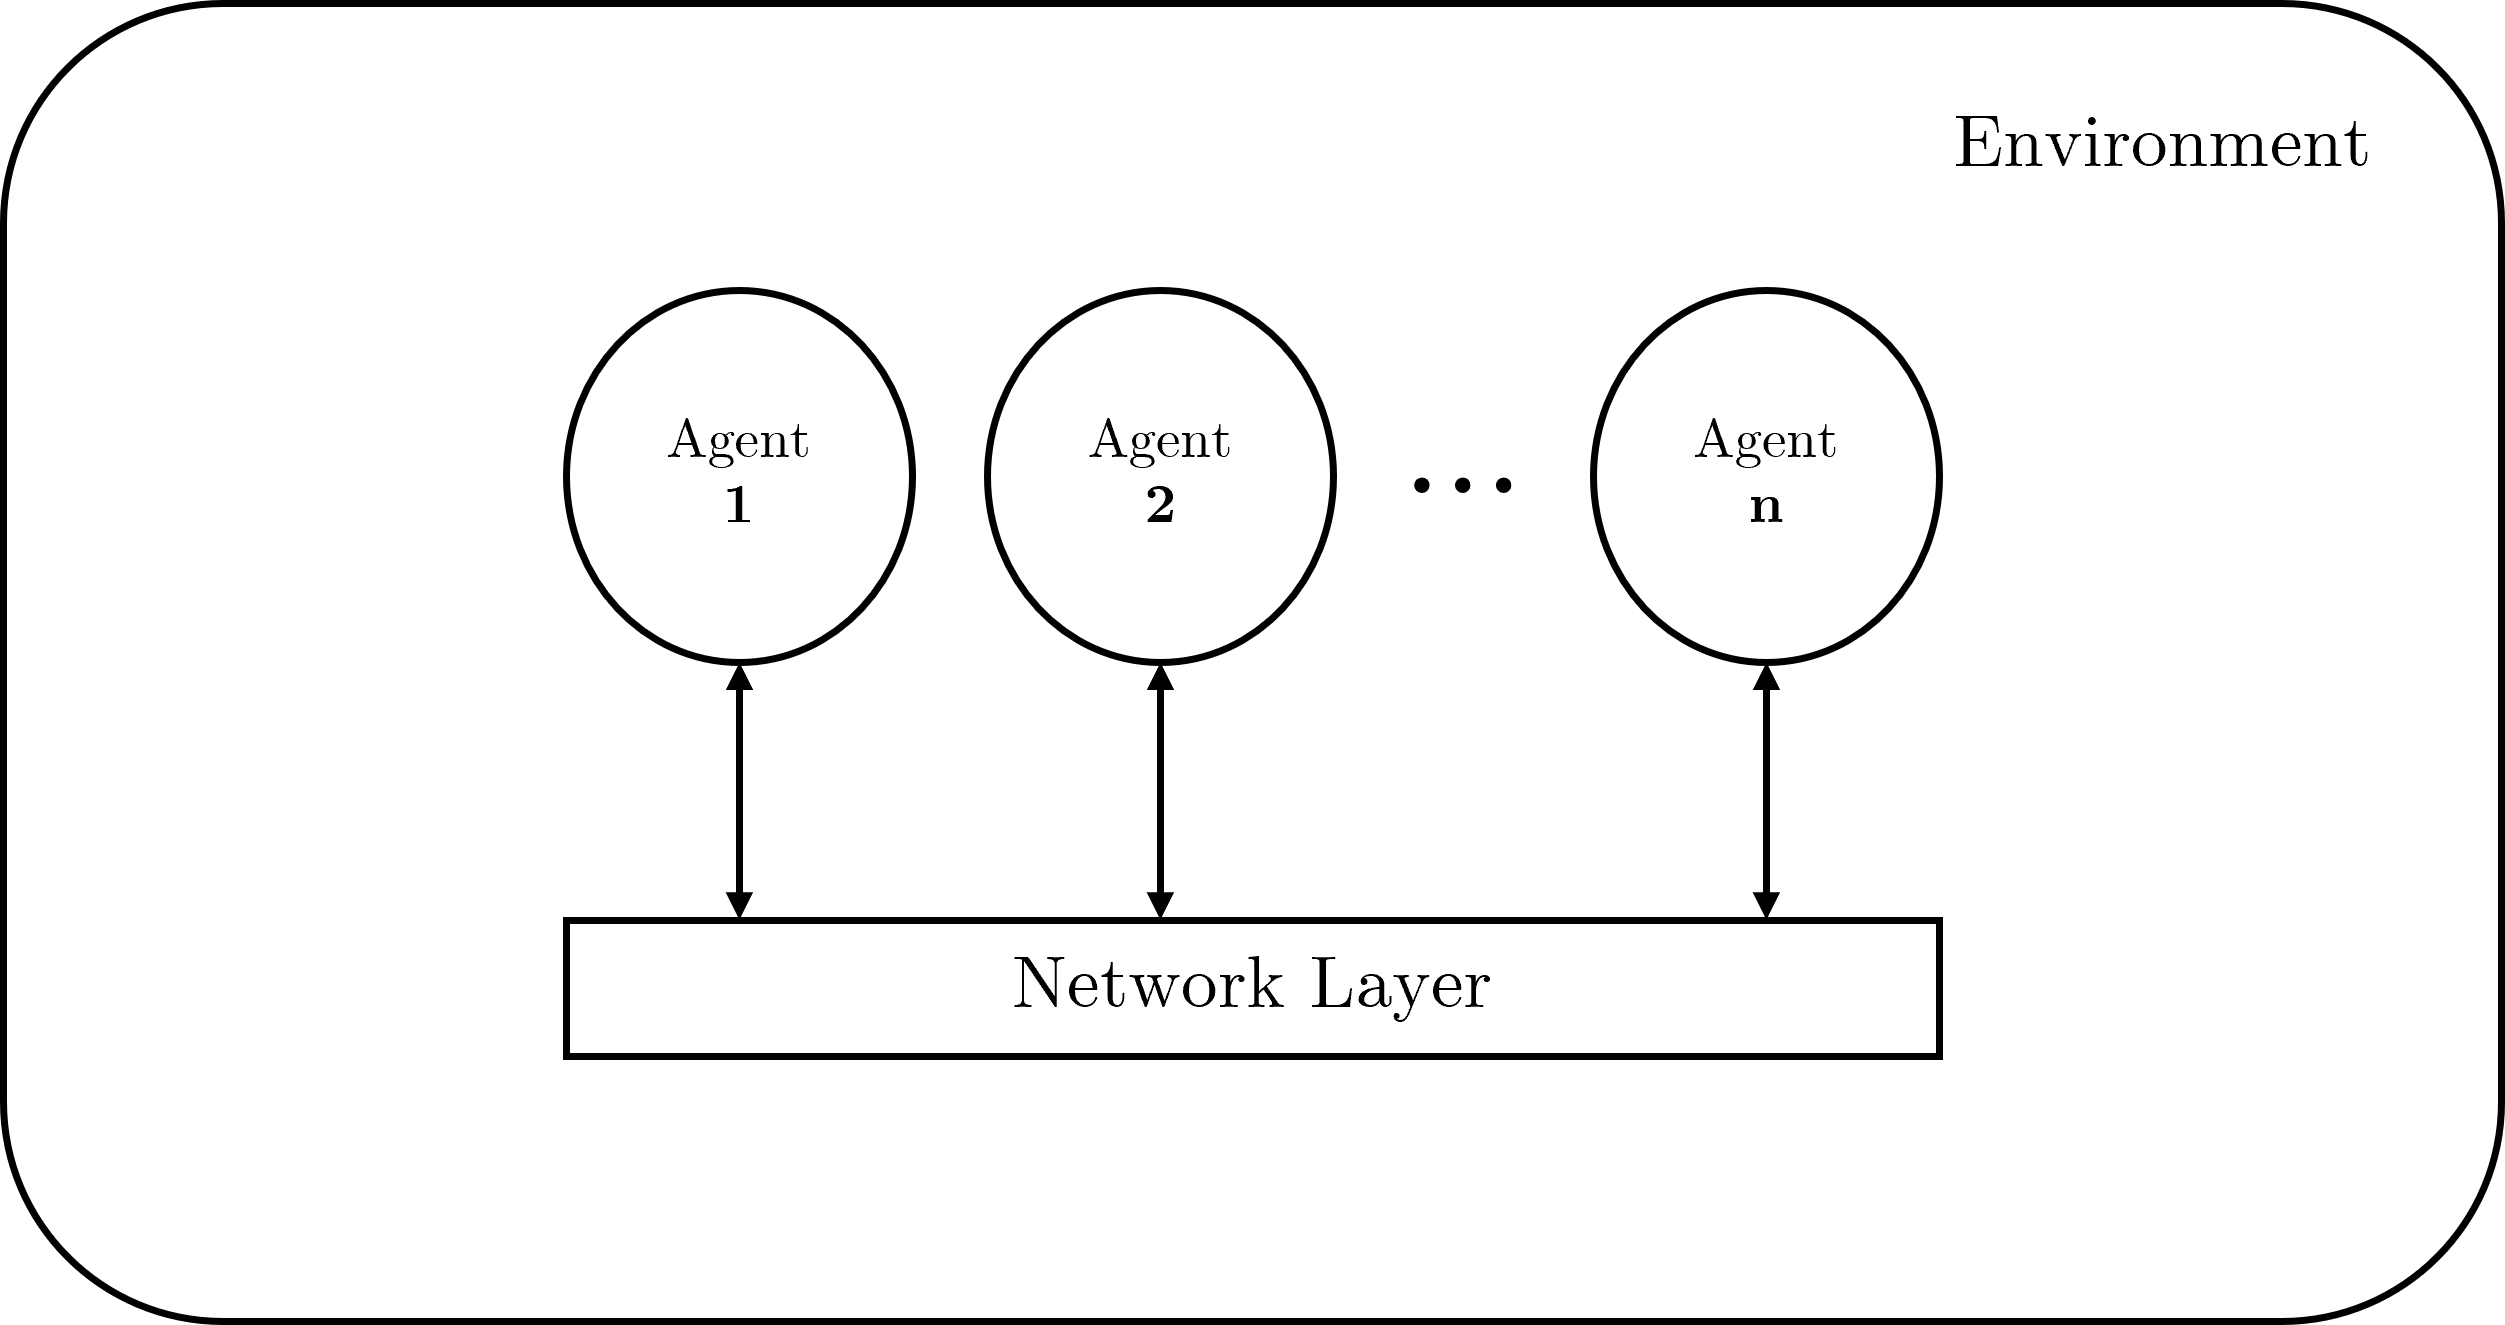
\includegraphics[width=0.50\textwidth]{images/network_layer.png}
    \caption{Example agents connected to a network layer.}
    \label{fig:network_layer_example}
\end{figure}

Therefore, each agent still trains independently and selects their optimal policy $\pi^*$, or rather, action depending on the algorithm used. The network layer provides the foundations from which we can develop novel algorithms that utilise information from other agents.

\subsection{Communication Bus}

The key idea is to allow agents to communicate their local state information to neighbouring agents. This enables each agent to make decisions not only based on its own state, but also on the state of surrounding junctions.

To facilitate communication between agents, we introduce a shared data structure we refer to as a \emph{communication bus}, available to all agents that use the new algorithm. Each agent publishes its local state to the bus at every time step in the simulation, and can read the most recent states of other agents.

Let $s_{n_t}$ denote the standard local state of agent $n$ at time step $t$. Let $\mathcal{N}(n)$ denote the set of neighbouring agents to agent $n$. The new state ${s_{n_t}}^{comm}$ used by agent $n$ in their Communicative Deep Q-learning algorithm is defined as:

\[
{s_{n_t}}^{comm} = (s_{n_t},) +  (s_{j_{1_t}}, s_{j_{2_t}}, \dots, s_{j_{k_t}}) \quad \text{where } j \in \mathcal{N}(n)
\]

As shown, the communicative state is limited to the state of the agent concatenated with the local state tuples of the neighbouring agents. We have elected to only add neighbouring agents since it allows for complete decentralisation -- each agent only needs to be connected directly to adjacent agents, rather than needing to connect with all agents perhaps through a centralised server.

\begin{figure}[H]
    \centering
    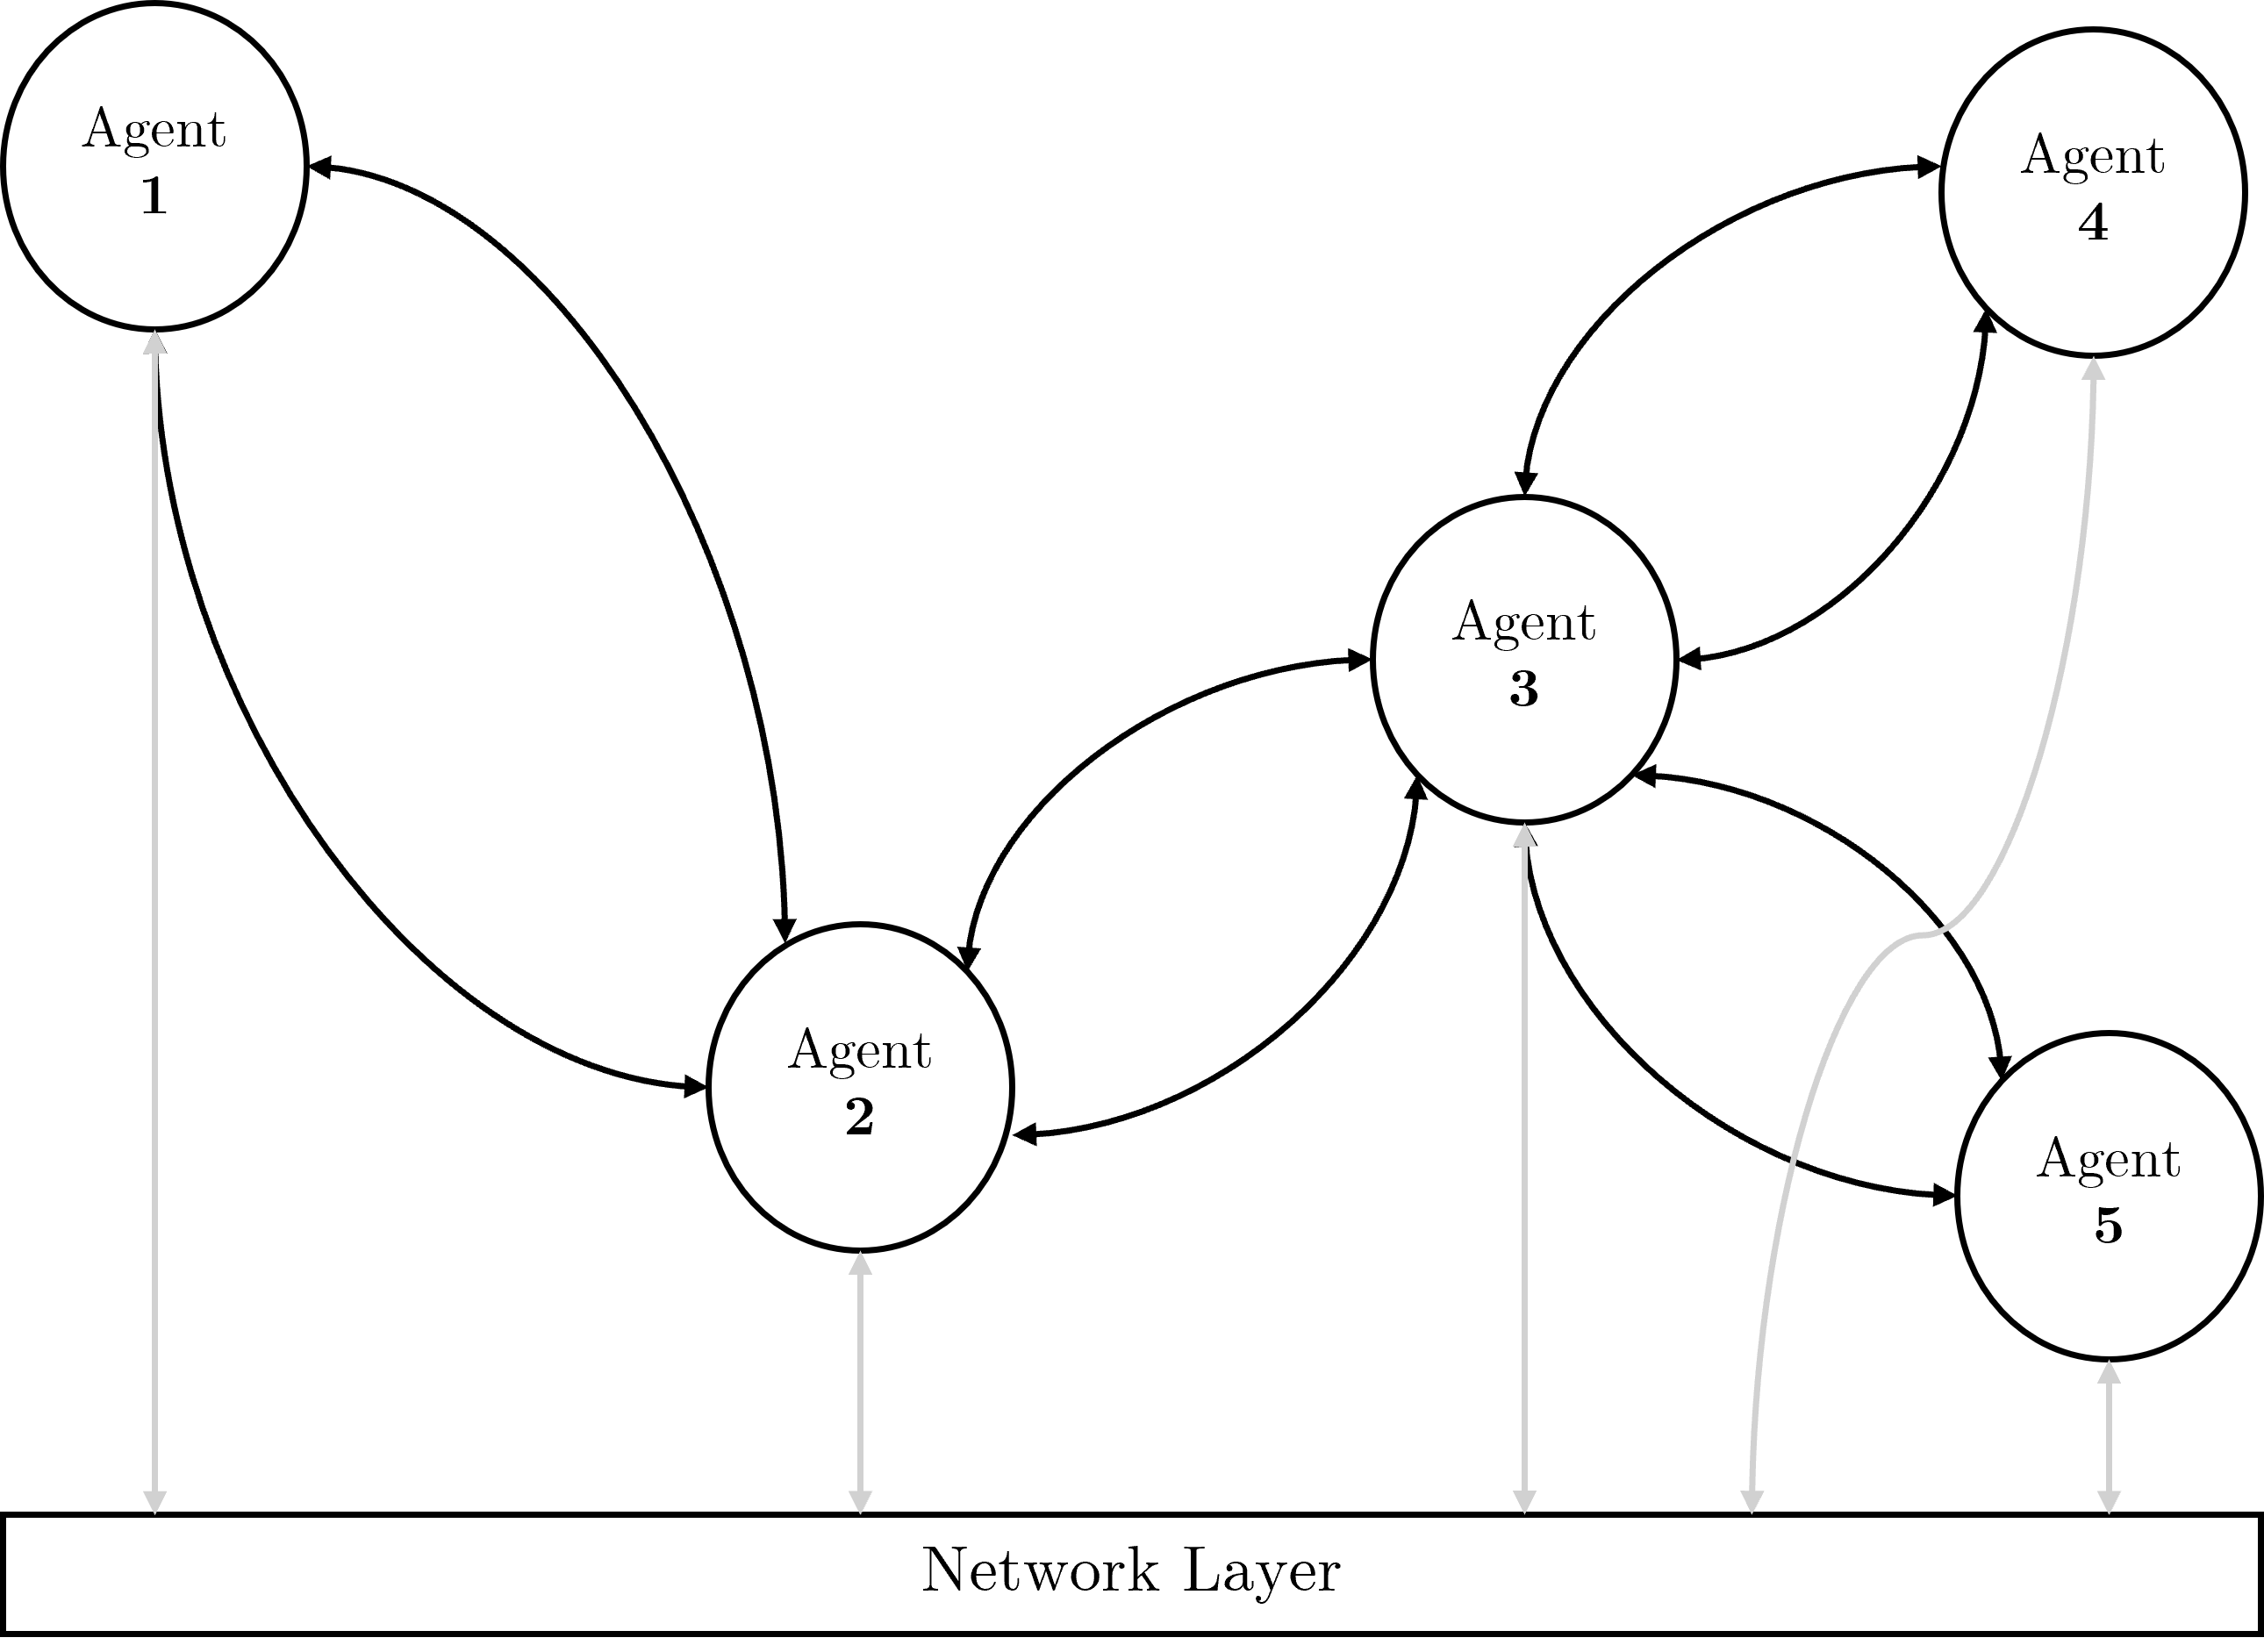
\includegraphics[width=0.50\textwidth]{images/communication_example.png}
    \caption{Abstracted example of agents communicating in a decentralised manner.}
    \label{fig:communication_example}
\end{figure}

In the abstracted example, you can imagine that the agents which are connected together control traffic lights which are directly adjacent to one another, sharing the same road. Communication is limited to state sharing only and there is no central controller making decisions.

\subsection{Algorithm}

\begin{algorithm}[H]
  \caption{Communicative Deep Q-Learning}
  \begin{algorithmic}[1]
  \State Initialise communication bus $B$
  \For{each agent $n$}
    \State Initialise replay buffer $D_n$
    \State Initialise policy DQN with weights $\theta_n$
    \State Initialise target network with weights $\theta_n^- \leftarrow \theta_n$
  \EndFor
  \For{each episode}
    \For{each agent $n$}
        \State Observe initial local state $s_n$
        \State Publish $s_n$ to bus $B$
    \EndFor
    \For{each step in episode}
      \For{each agent $n$}
        \State Read neighbour states $\{s_j \mid j \in \mathcal{N}(n)\}$ from $B$
        \State Construct communicative state: $s_n^{comm} = (s_n, s_{j_1}, s_{j_2}, \dots, s_{j_k})$
        \State Select action $a_n$ using $\epsilon$-greedy policy on $Q(s_n^{comm}, \cdot; \theta_n)$
        \State Set action $a_n$ using traffic light controller $\text{TLS}_n$
      \EndFor

      \State Execute one step in the environment simulation

      \For{each agent $n$}
        \State Observe reward $R_n$, next state $s'_n$, duration $d_n$
        \State Publish $s'_n$ to bus $B$
        \State Read neighbour next states $\{s'_j\}$ from $B$
        \State Construct next communicative state: ${s'_n}^{comm} = (s'_n, s'_{j_1}, \dots, s'_{j_k})$
        \State Store transition: $(s_n^{comm}, a_n, R_n, {s'_n}^{comm}, d_n, \delta_n) \in D$
        \State Sample minibatch from $D$
        \For{each sample $(s_i, a_i, R_i, s'_i, \delta_i, d_i)$}
          \State $y_i \leftarrow R_i + (1 - \delta_i)\,\gamma^{d_i} \underset{a'}\max Q(s'_i, a'; \theta_n^-)$
        \EndFor
        \State Perform gradient descent on: $L(\theta_n) = \frac{1}{b} \sum_{i=1}^{b} \left(y_i - Q(s_i, a_i; \theta_n)\right)^2$
        \State Update state $s_n \leftarrow s'_n$
        \State Periodically update target network: $\theta_n^- \leftarrow \theta_n$
      \EndFor
    \EndFor
  \EndFor
  \end{algorithmic}
\end{algorithm}

The algorithm\footnotemark\footnotetext{This pseudocode has some omissions, namely agents complete \emph{multi-step} actions that can finish at \emph{differing} times, therefore additional code is needed to monitor an action's progress.} extends the Deep Q-Learning algorithm. Rather than only running a single agent, we now iterate through and run an indefinite number. The \emph{network layer} we mentioned previously is \emph{where} this algorithm code exists. In other words, the set of agents exist on top of the network layer.

We first set up the communication bus $B$, which maintains a map of key-value pairs, where the keys are the agent IDs and the values are the most recent local state observation $s$ for each agent. We manually define the set of neighbours $\mathcal{N}$ for each agent ID (based on the topology of the traffic lights in the SUMO environment) such that agents can only retrieve their neighbours' state from the bus.

The agents are set up with similar parameters to before, except the input to the neural network for each agent is now $s^{comm}$ as opposed to $s$. At each step, the agents retrieve neighbouring state information from the bus to construct $s^{comm}$, and publish their own state $s$ so neighbours can do the same.

In a tangible implementation, a main benefit of Communicative Deep Q-learning comes from it being decentralised. Although necessary for the code, in practice, a network layer and the centralised communication bus $B$ our agents interface with wouldn't exist. Instead, the bus interface would be replaced with physical (e.g.\ copper) cables connected only with nearby adjacent agents.

\subsection{Implementation}

Enabling communication between agents required a significant rework of the code. Some changes below were retroactively added to the previous algorithm sections since it makes for easier understanding.

Initially only one agent was allowed since it, in essence, was the primary driver of the SUMO simulation -- it directly made \texttt{simulationStep()} interface calls to advance the simulation forward. Multiple agents was not possible for there was no encapsulation to delimit what an agent was.

This necessitated the \texttt{Controller} class in the \texttt{Environment} package, which has a one-to-one mapping with each agent, encapsulated now as a \texttt{Runner} class. Each \texttt{Controller} keeps track of an agent's action and sets the corresponding TLS phase via a \texttt{setPhase()} interface call to SUMO, but it does \emph{not} step the simulation.

Simulation stepping was decoupled into a separate function exposed by the \texttt{Environment}. This is reserved and called solely by the \texttt{Network} layer class that is responsible for setting up multiple \texttt{Runner} classes.

\begin{figure}[H]
    \centering
    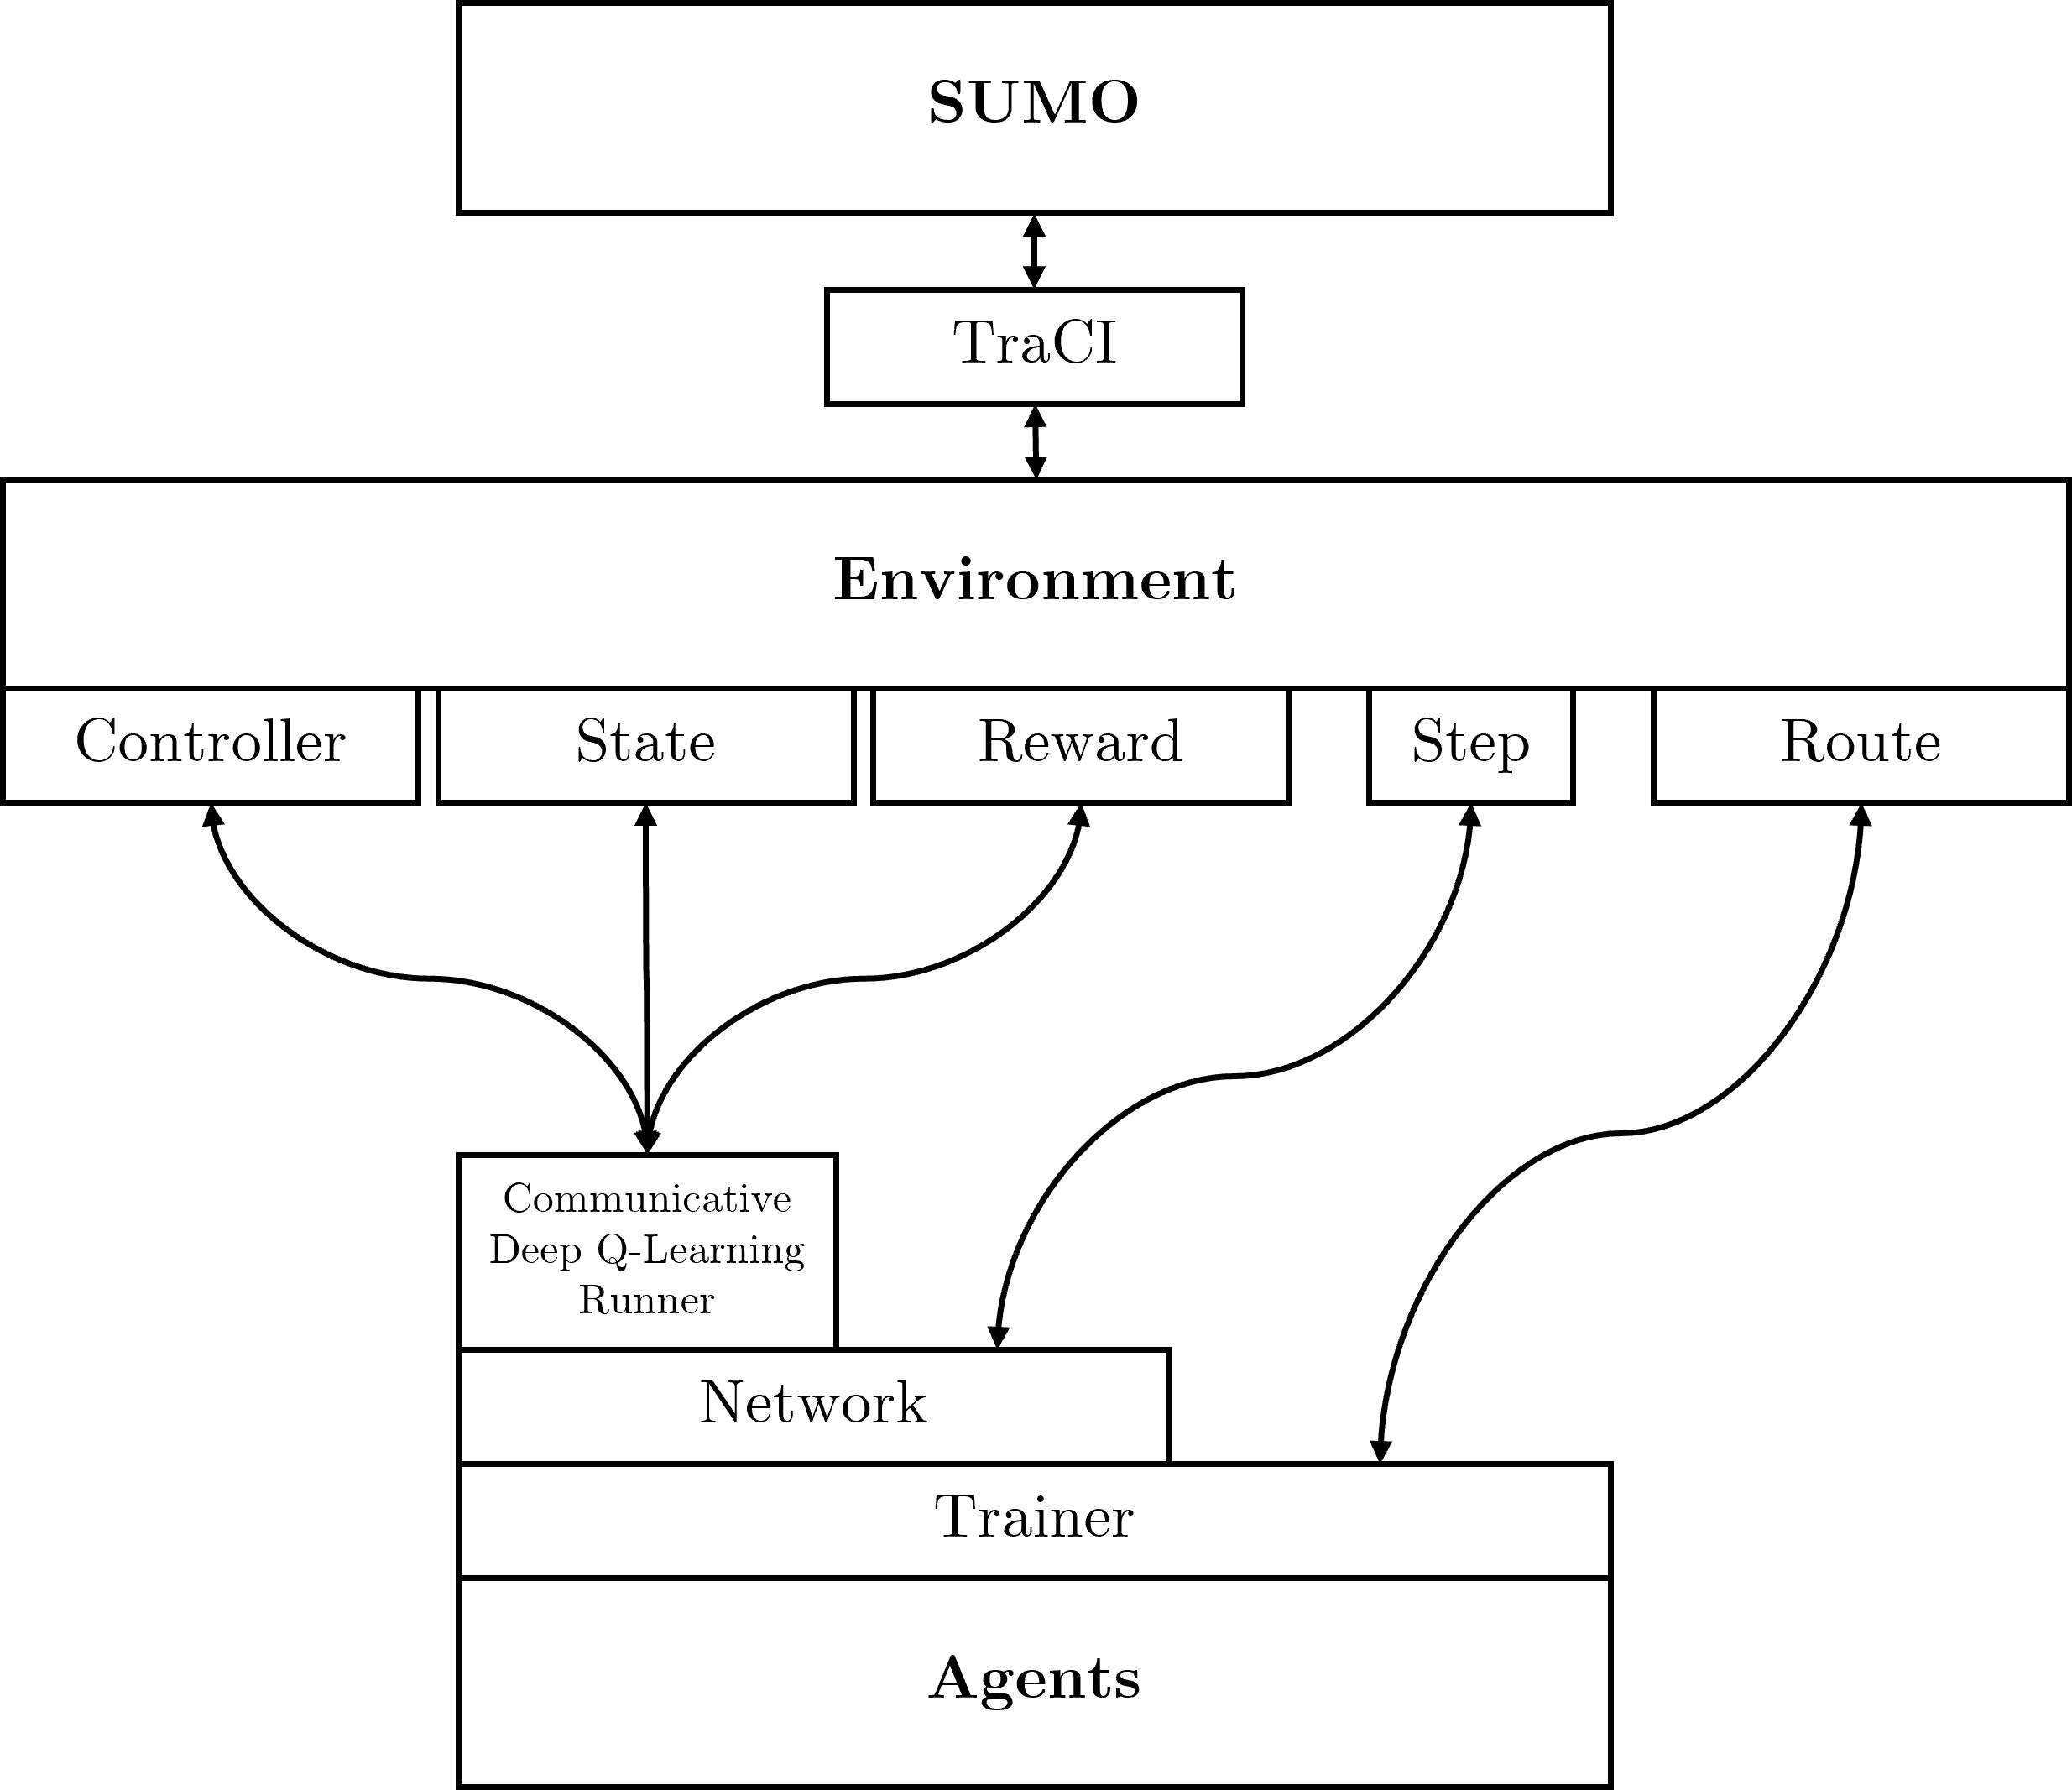
\includegraphics[width=0.64\textwidth]{images/implementation_extended.png}
    \caption{Library interactions and hierarchy of classes.}
    \label{fig:implementation_extended}
\end{figure}

The internal DQN architecture agents use was expanded, since the state for each agent -- and therefore the DQN input layers -- now included extra information from neighbouring agents. Rather than just two intermediary hidden layers of 64 nodes each, we replace this with three intermediary layers which progressively decrease in size: 256 nodes, 128 nodes, 64 nodes. The final output layer of $a$ actions remains as before.

\section{Extended Network}

To train the Communicative Deep Q-learning algorithm, we will construct a new environment which contains multiple traffic light systems. This is necessary since our previous networks contained only one traffic light system, but we need multiple for there to be communication. Our new network -- `extended network' -- will extend the original demo network. We replace the zebra crossing in \emph{Torrington Place} with a traffic light system, similar to what we done for the crossing network. 

\begin{figure}[H]
    \centering
    \begin{subfigure}{0.48\textwidth}
        \centering
        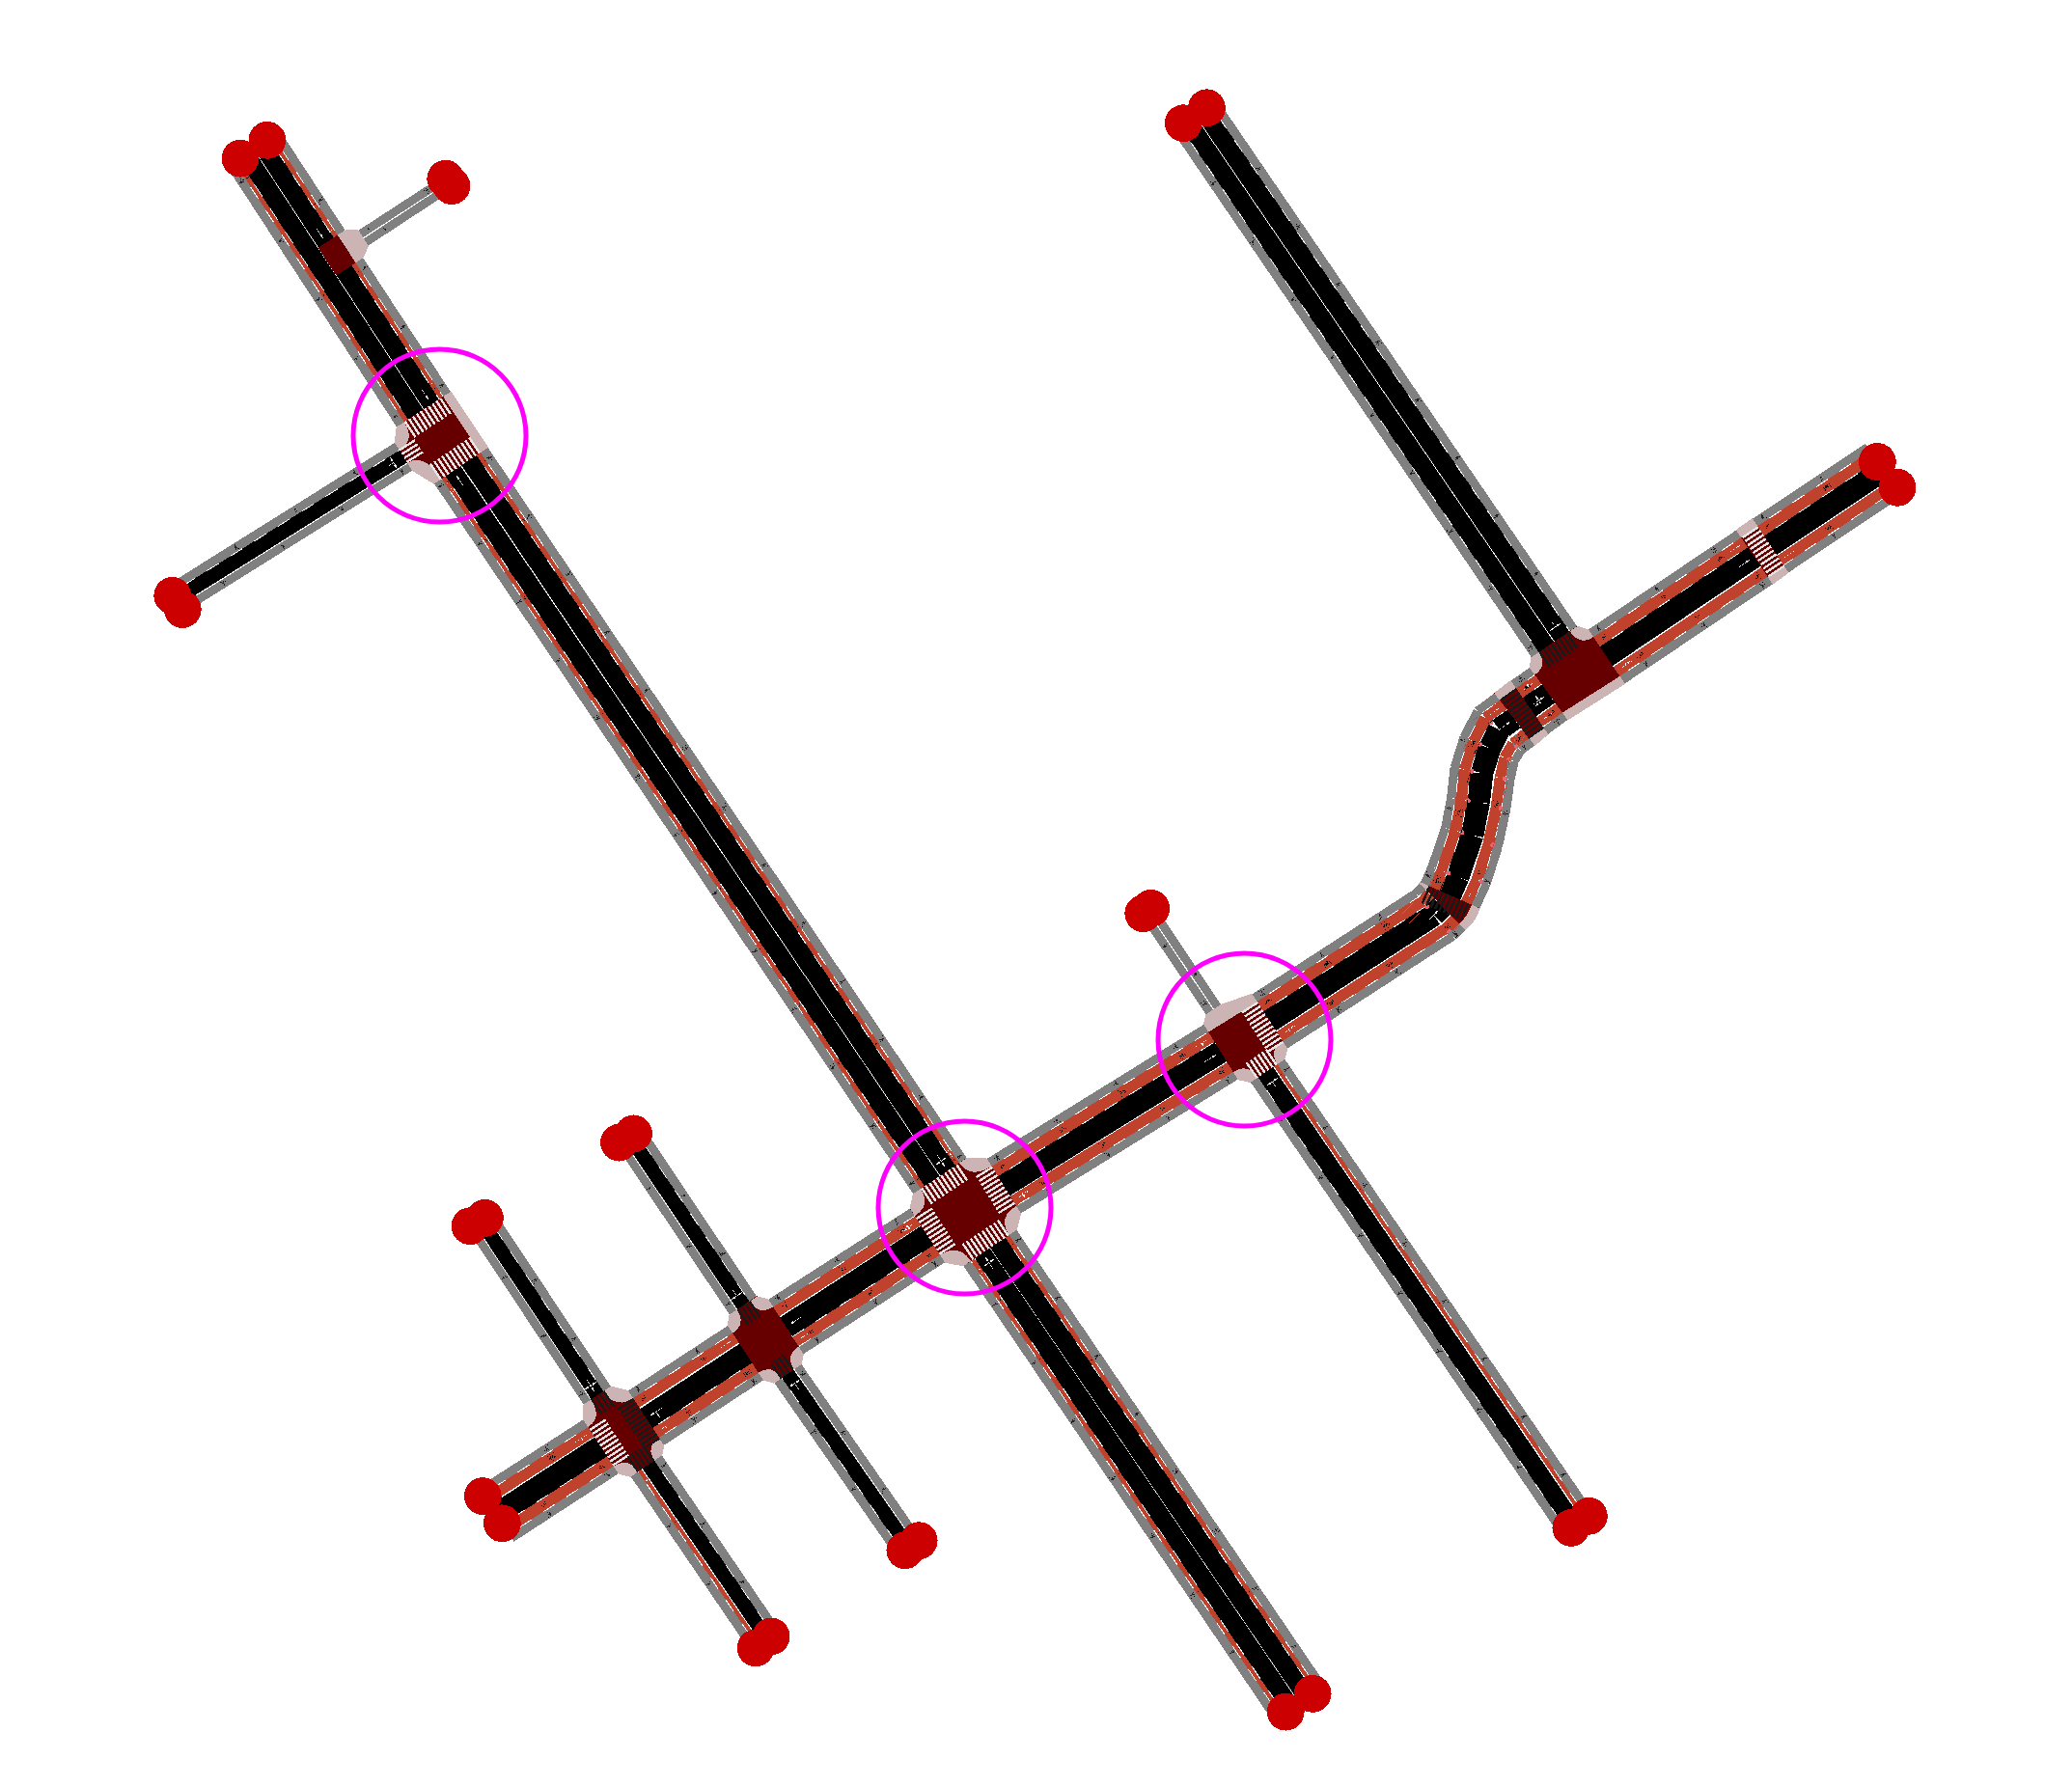
\includegraphics[width=\textwidth]{images/netedit_extended.png}
        \caption{Road network in netedit.}
        \label{fig:netedit_extended}
    \end{subfigure}
    \hfill
    \begin{subfigure}{0.48\textwidth}
        \centering
        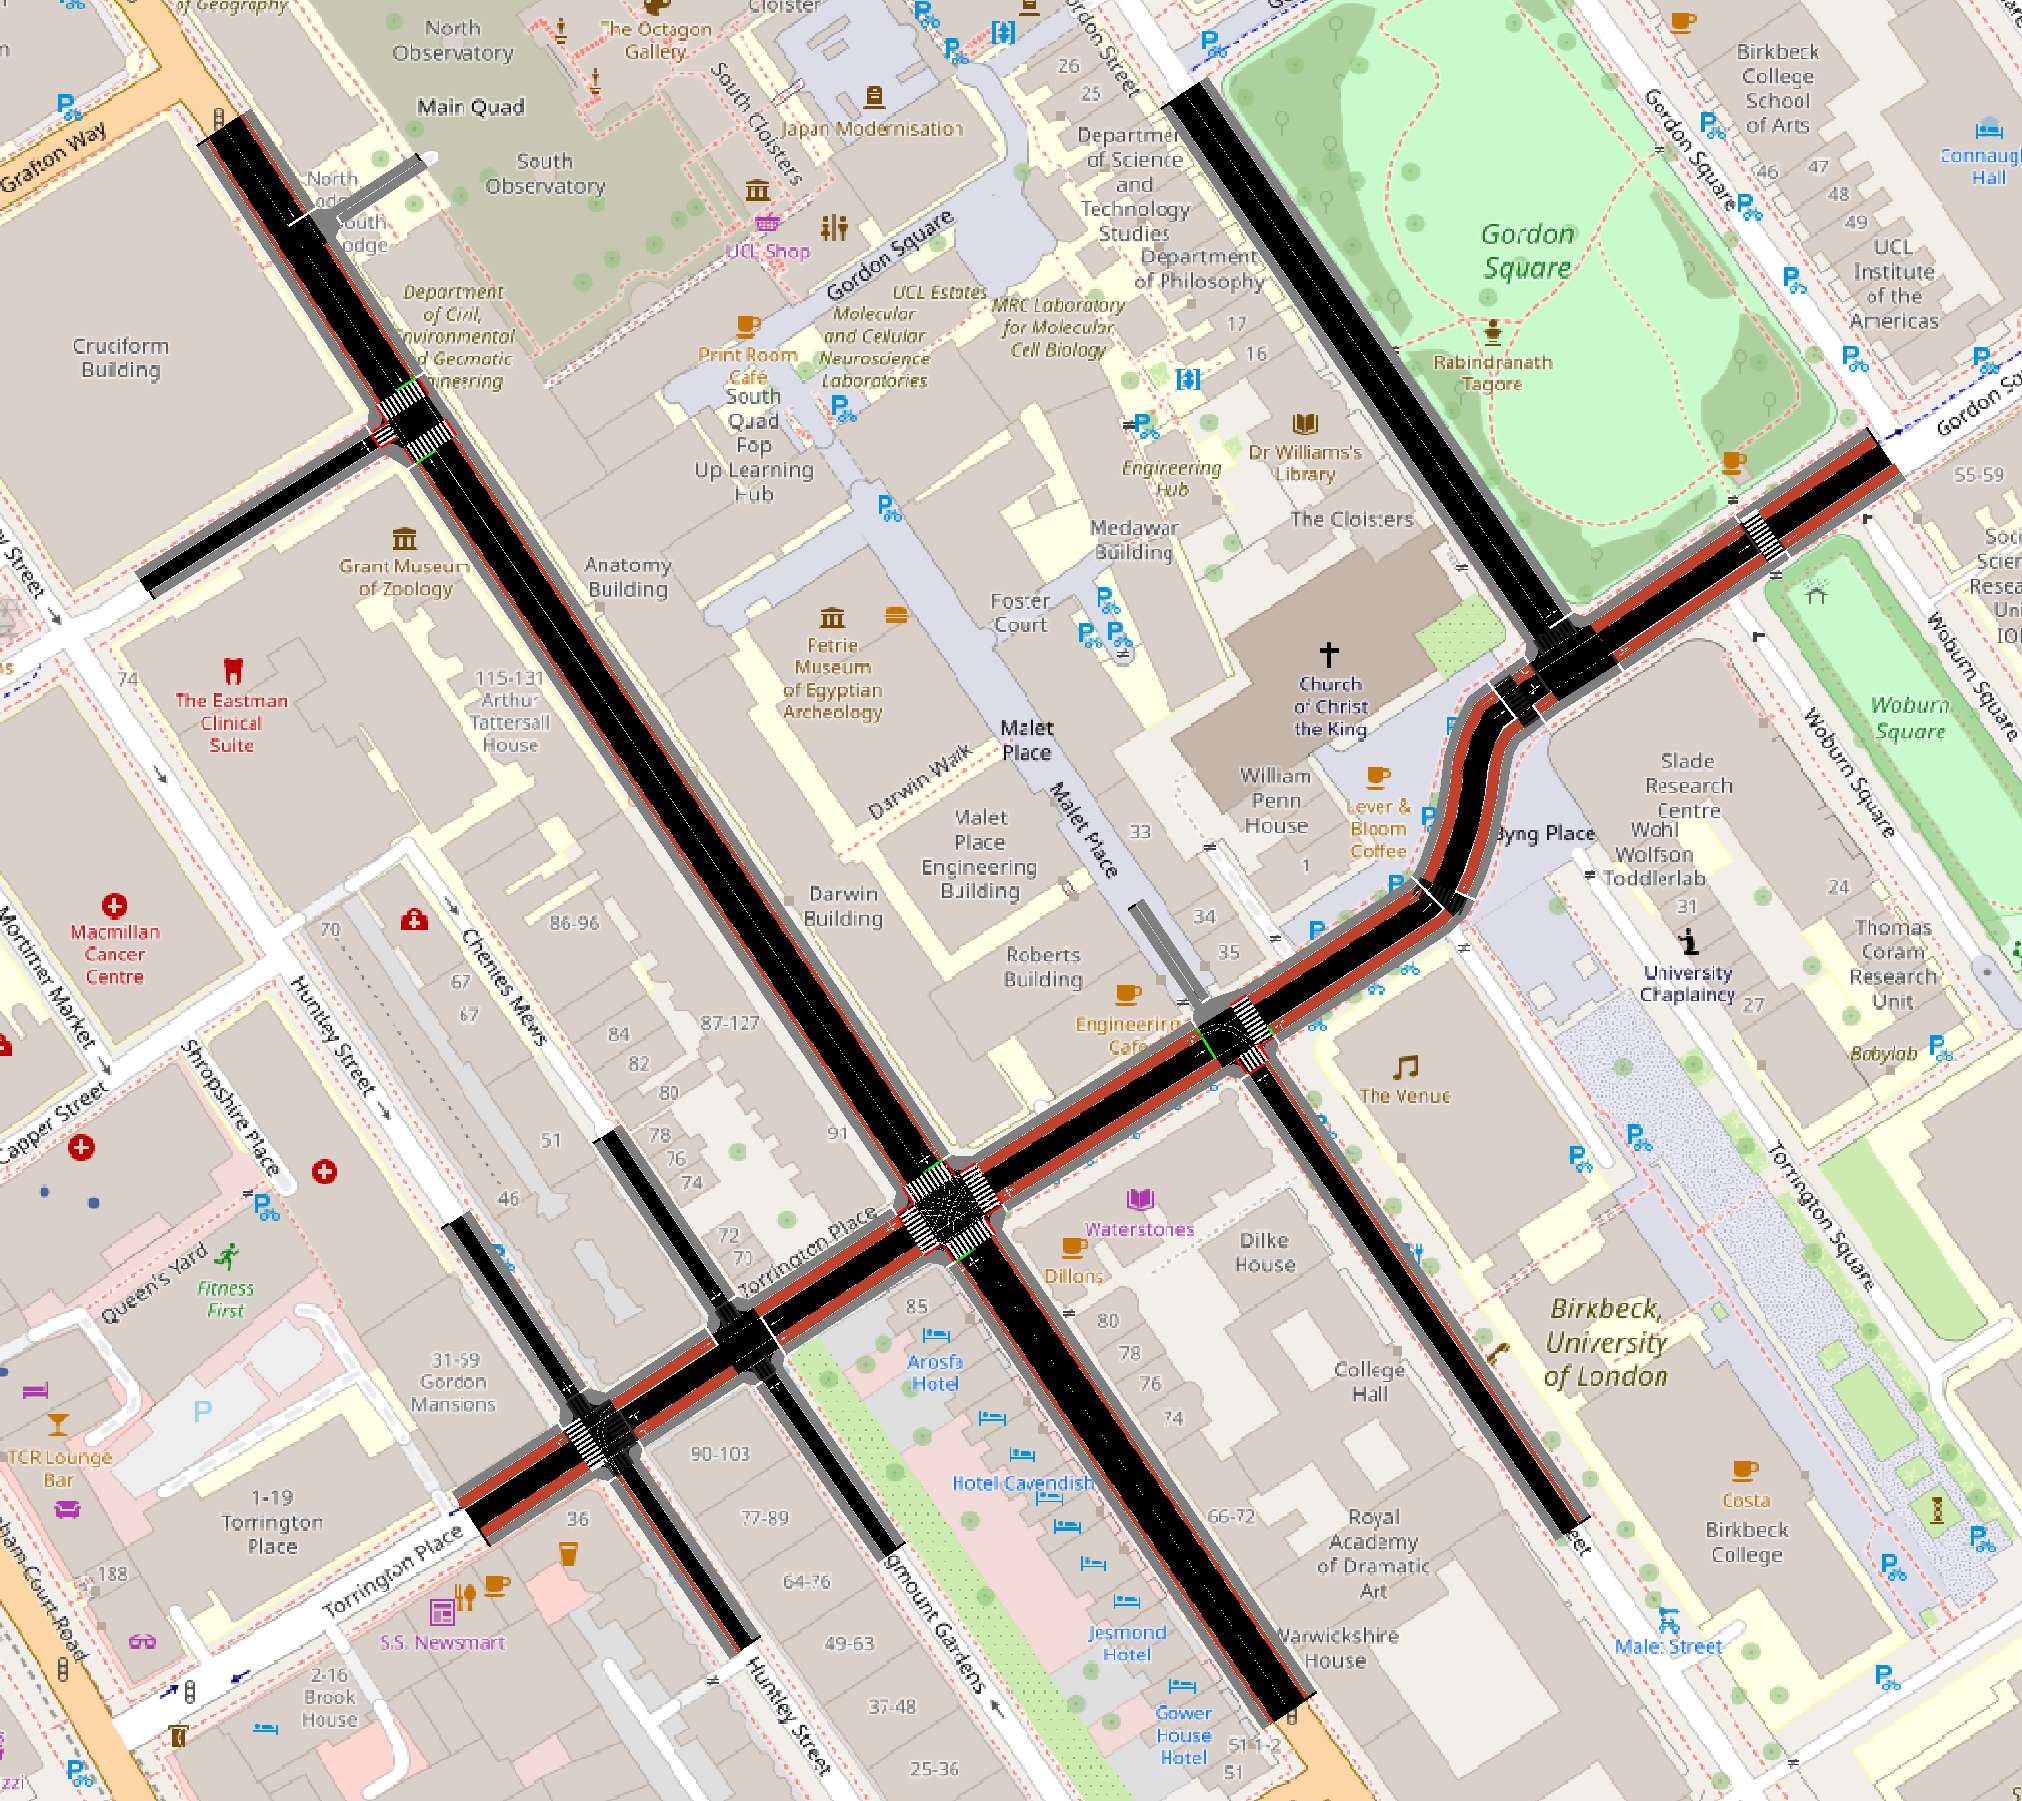
\includegraphics[width=\textwidth]{images/sumo_extended.png}
        \caption{Simulation view in SUMO.}
        \label{fig:sumo_extended}
    \end{subfigure}
    \caption{Extended simulation environment.}
    \label{fig:extended_simulation}
\end{figure}

As seen in Figure~\ref{fig:sumo_extended}, the network now includes three traffic light systems. This means that we will have three respective agents that will be publishing to the communication bus $B$. Although it would be ideal to have a much larger network, we will limit the scope for the sake of this dissertation and evaluate in a smaller environment.

Each of three agents train independently using the detectors and state from their own traffic light system. The detectors are configured in a different manner for each traffic light system. The middle traffic light in Figure~\ref{fig:netedit_extended} will be \emph{TLS 1}, the rightmost will be \emph{TLS 2}, and the leftmost will be \emph{TLS 3}. 

\begin{figure}[H]
    \centering
    \begin{subfigure}{0.30\textwidth}
        \centering
        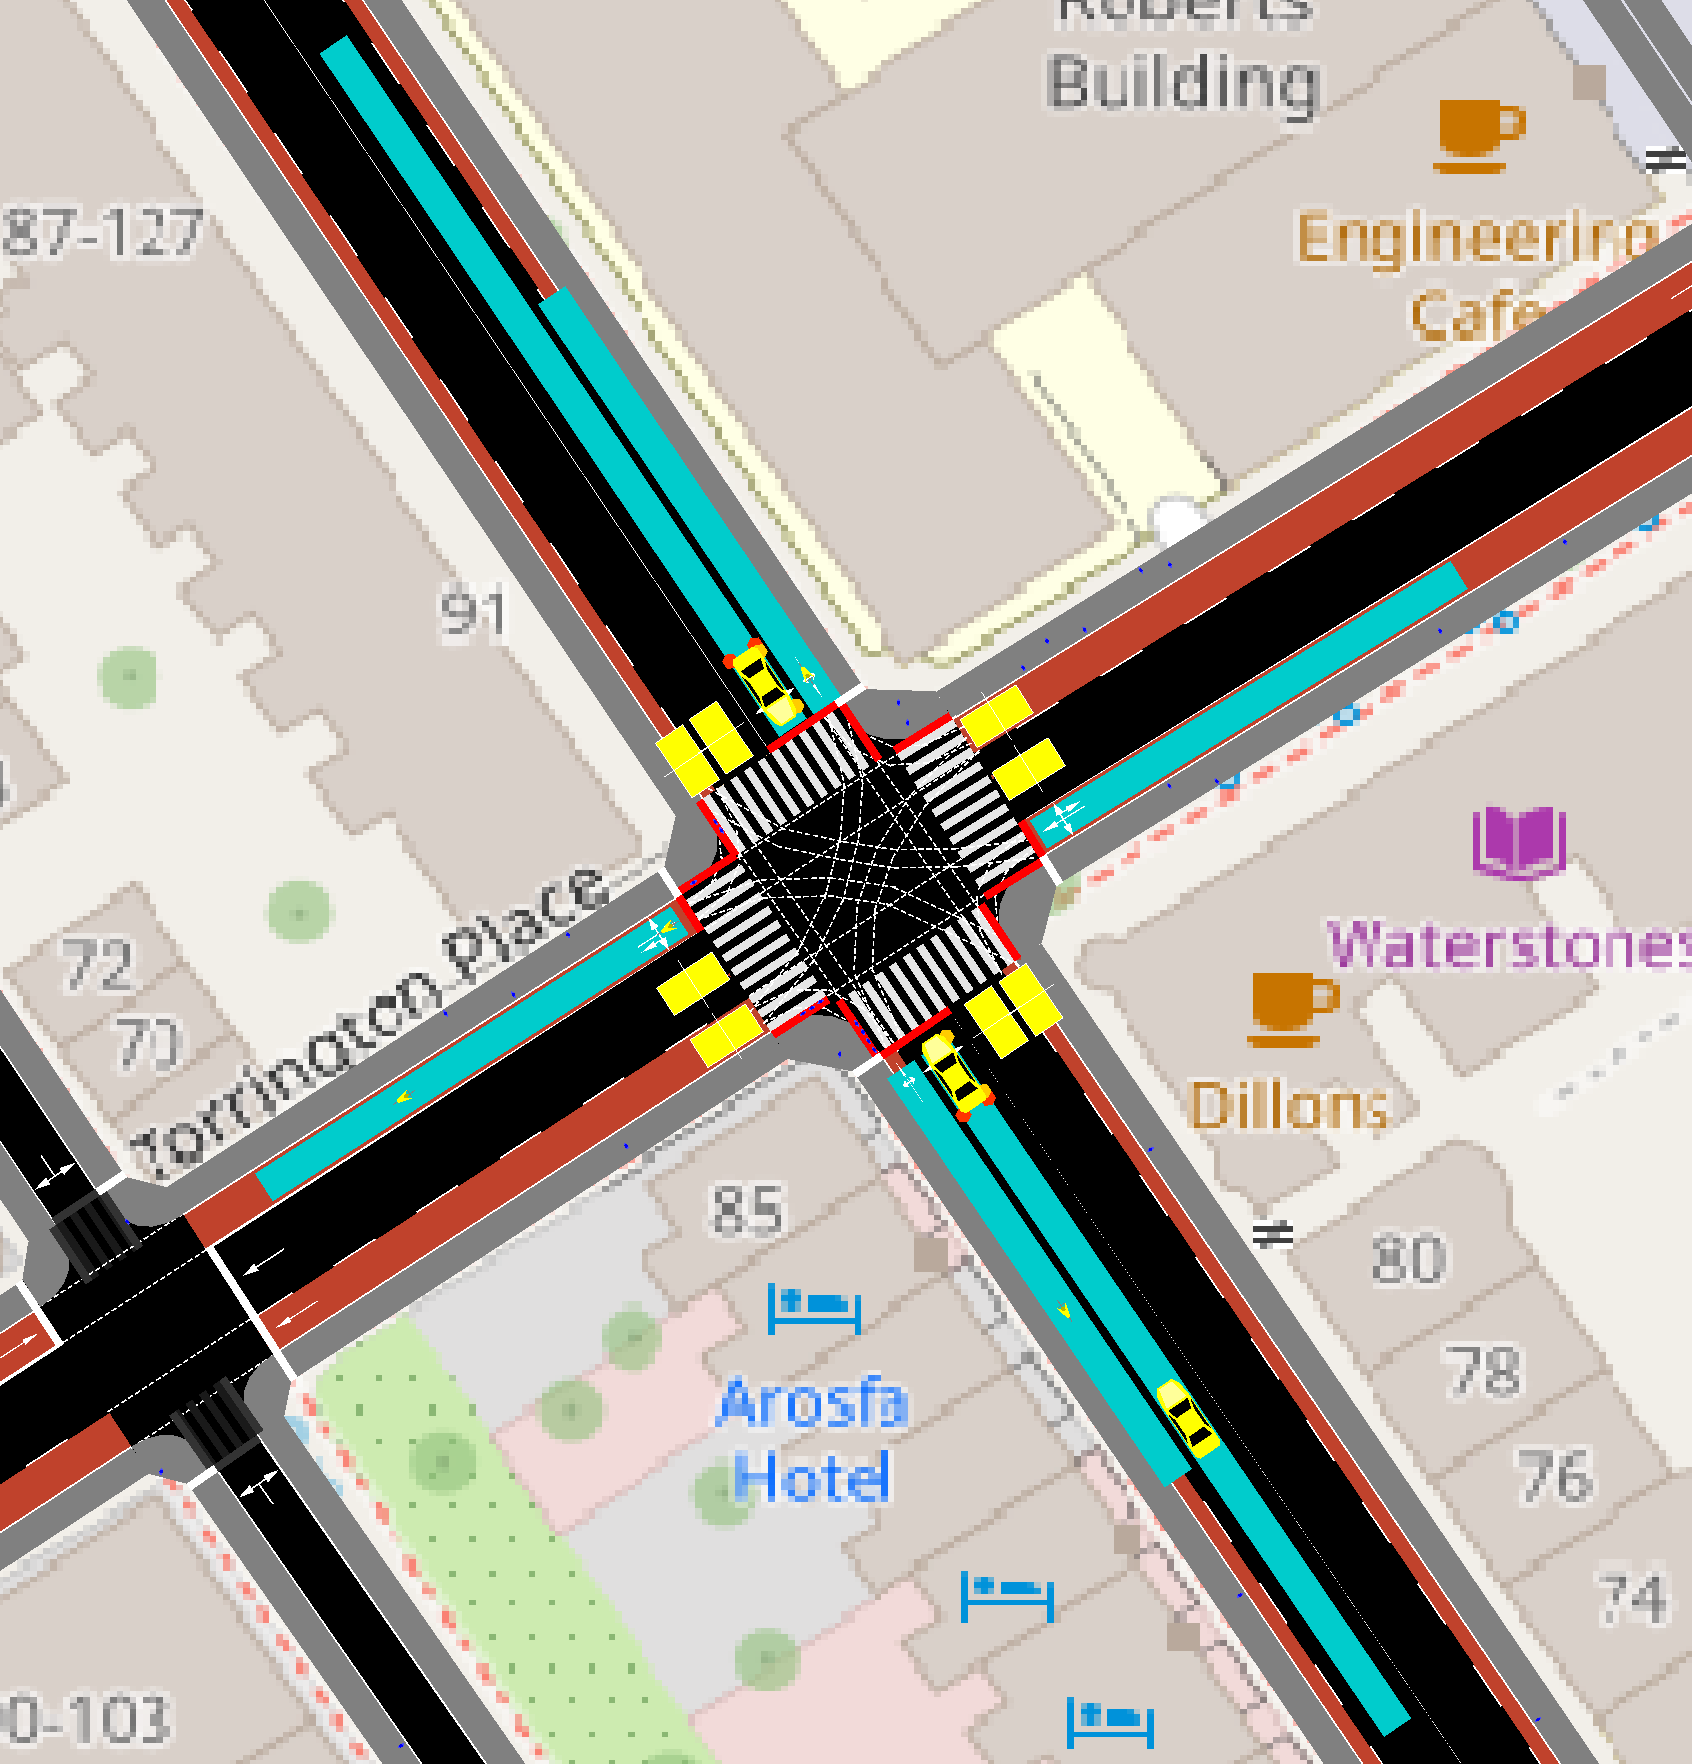
\includegraphics[width=\textwidth]{images/detectors_demo.png}
        \caption{TLS 1.}
    \end{subfigure}
    \hfill
    \begin{subfigure}{0.30\textwidth}
        \centering
        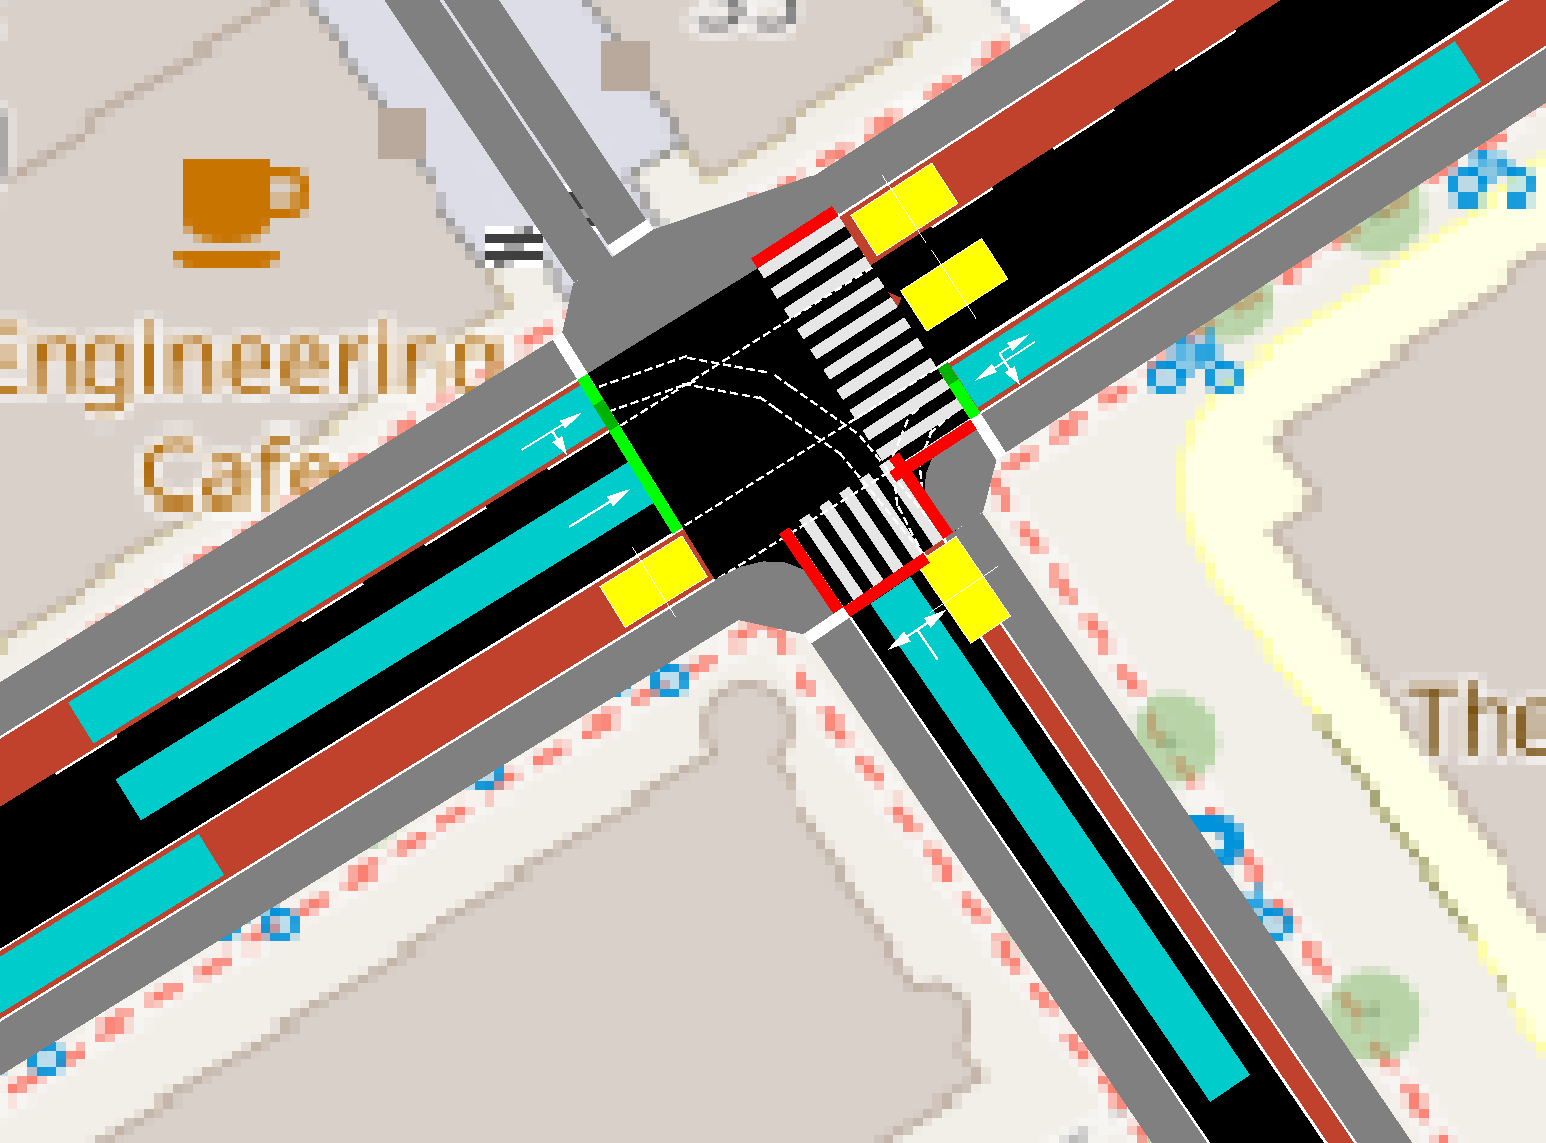
\includegraphics[width=\textwidth]{images/detectors_crossing.png}
        \caption{TLS 2.}
    \end{subfigure}
    \hfill
    \begin{subfigure}{0.30\textwidth}
        \centering
        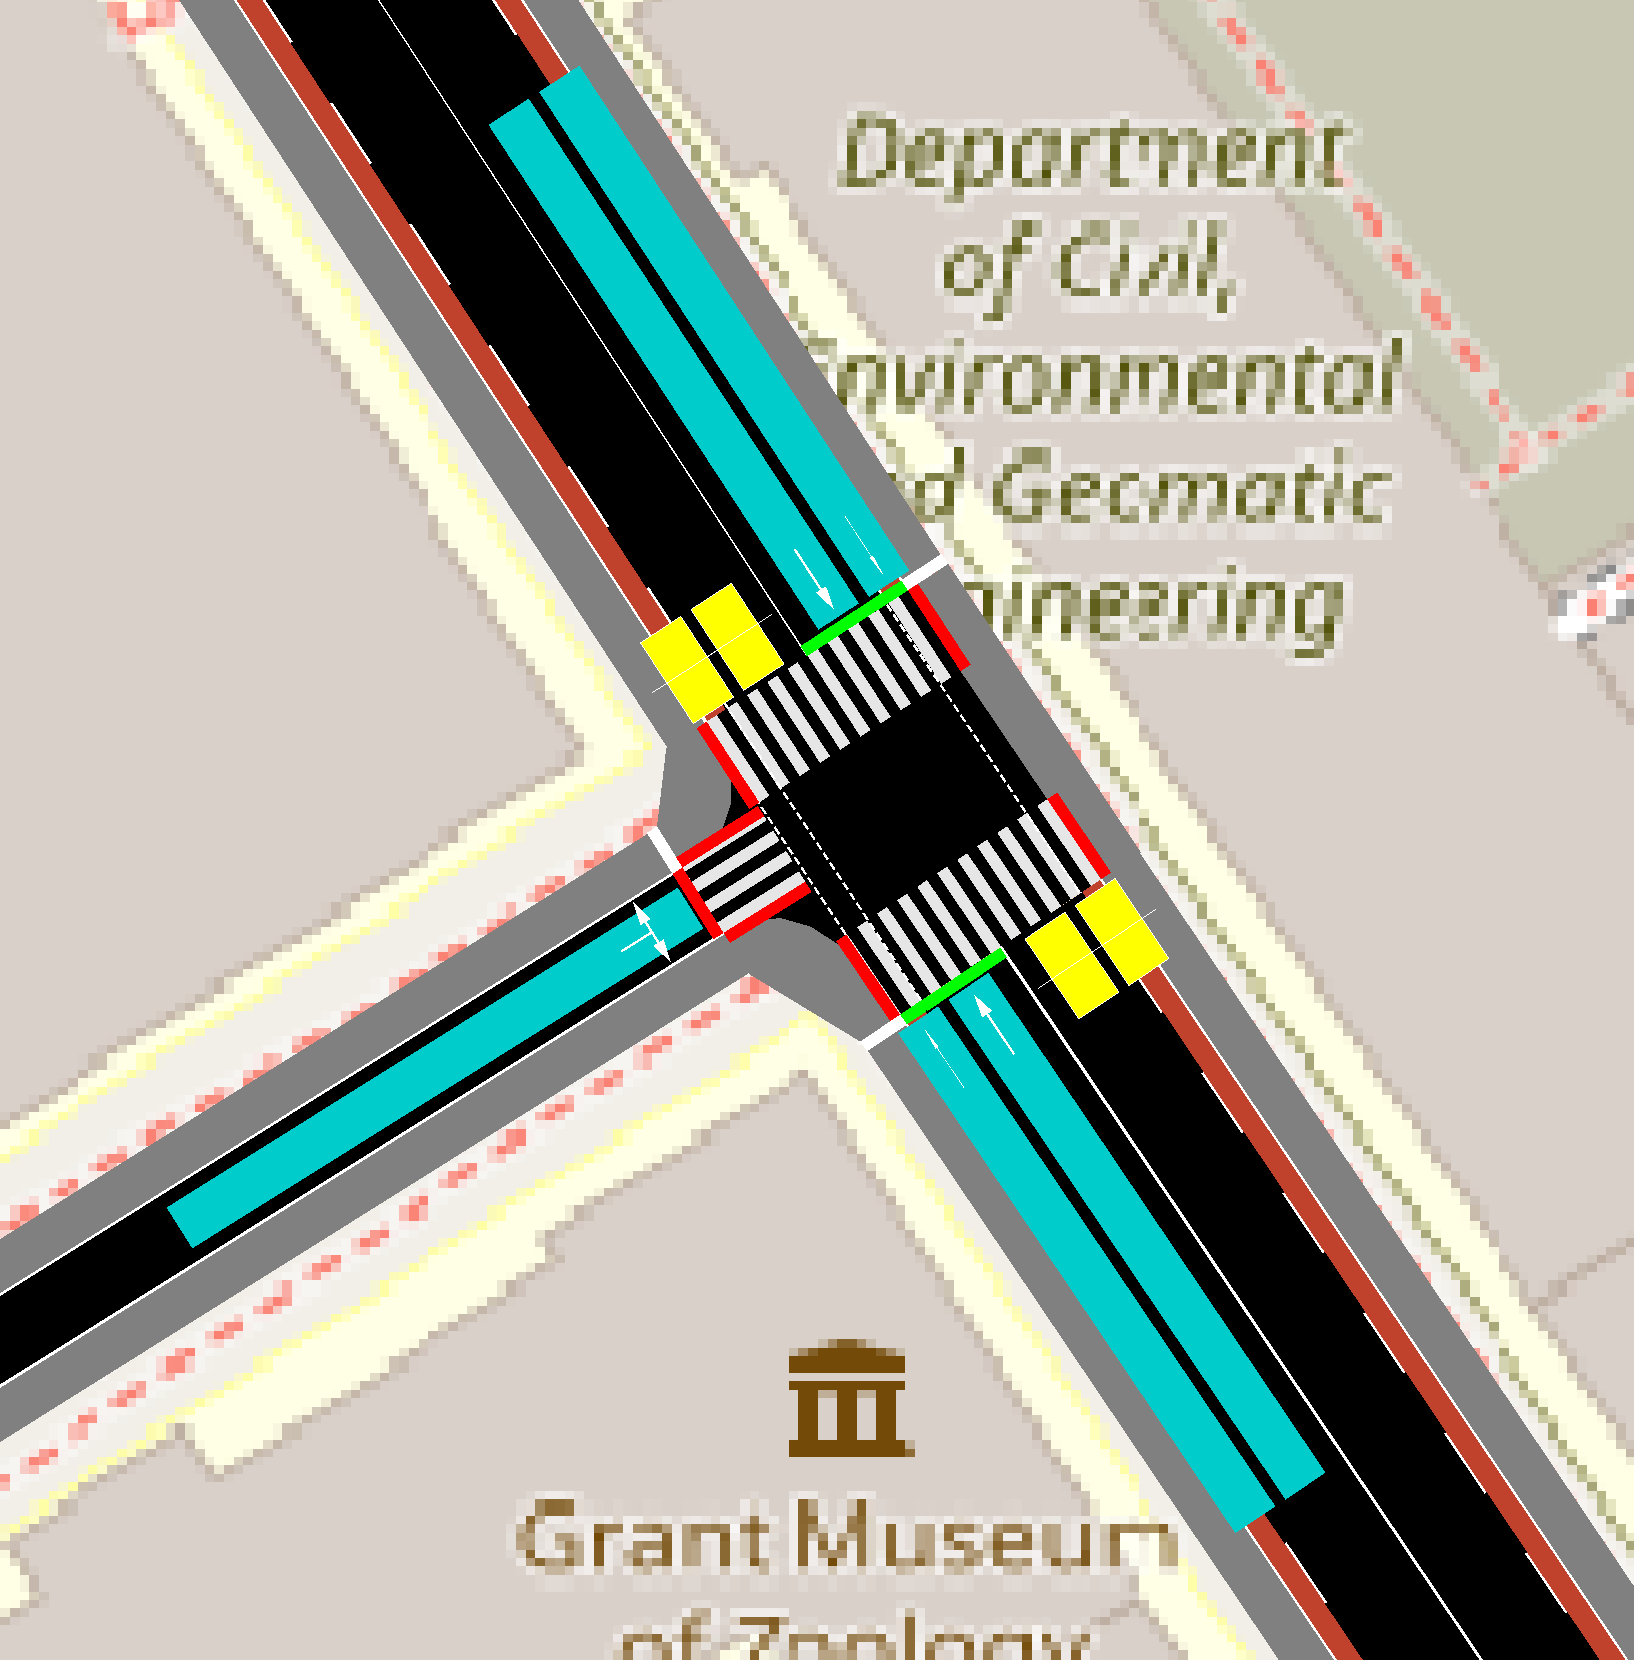
\includegraphics[width=\textwidth]{images/detectors_extended.png}
        \caption{TLS 3.}
    \end{subfigure}
    \caption{Detectors in the extended network.}
    \label{fig:detectors_extended}
\end{figure}

The state tuple for each is also unique. TLS 1 will have a state tuple of 15 elements, TLS 2 will have a state tuple of 9 elements, and TLS 3 will have a state tuple of 12 elements, using the general formula defined in \eqref{state_formula}.

\begin{figure}[H]
    \centering
    \begin{subfigure}{0.30\textwidth}
        \centering
        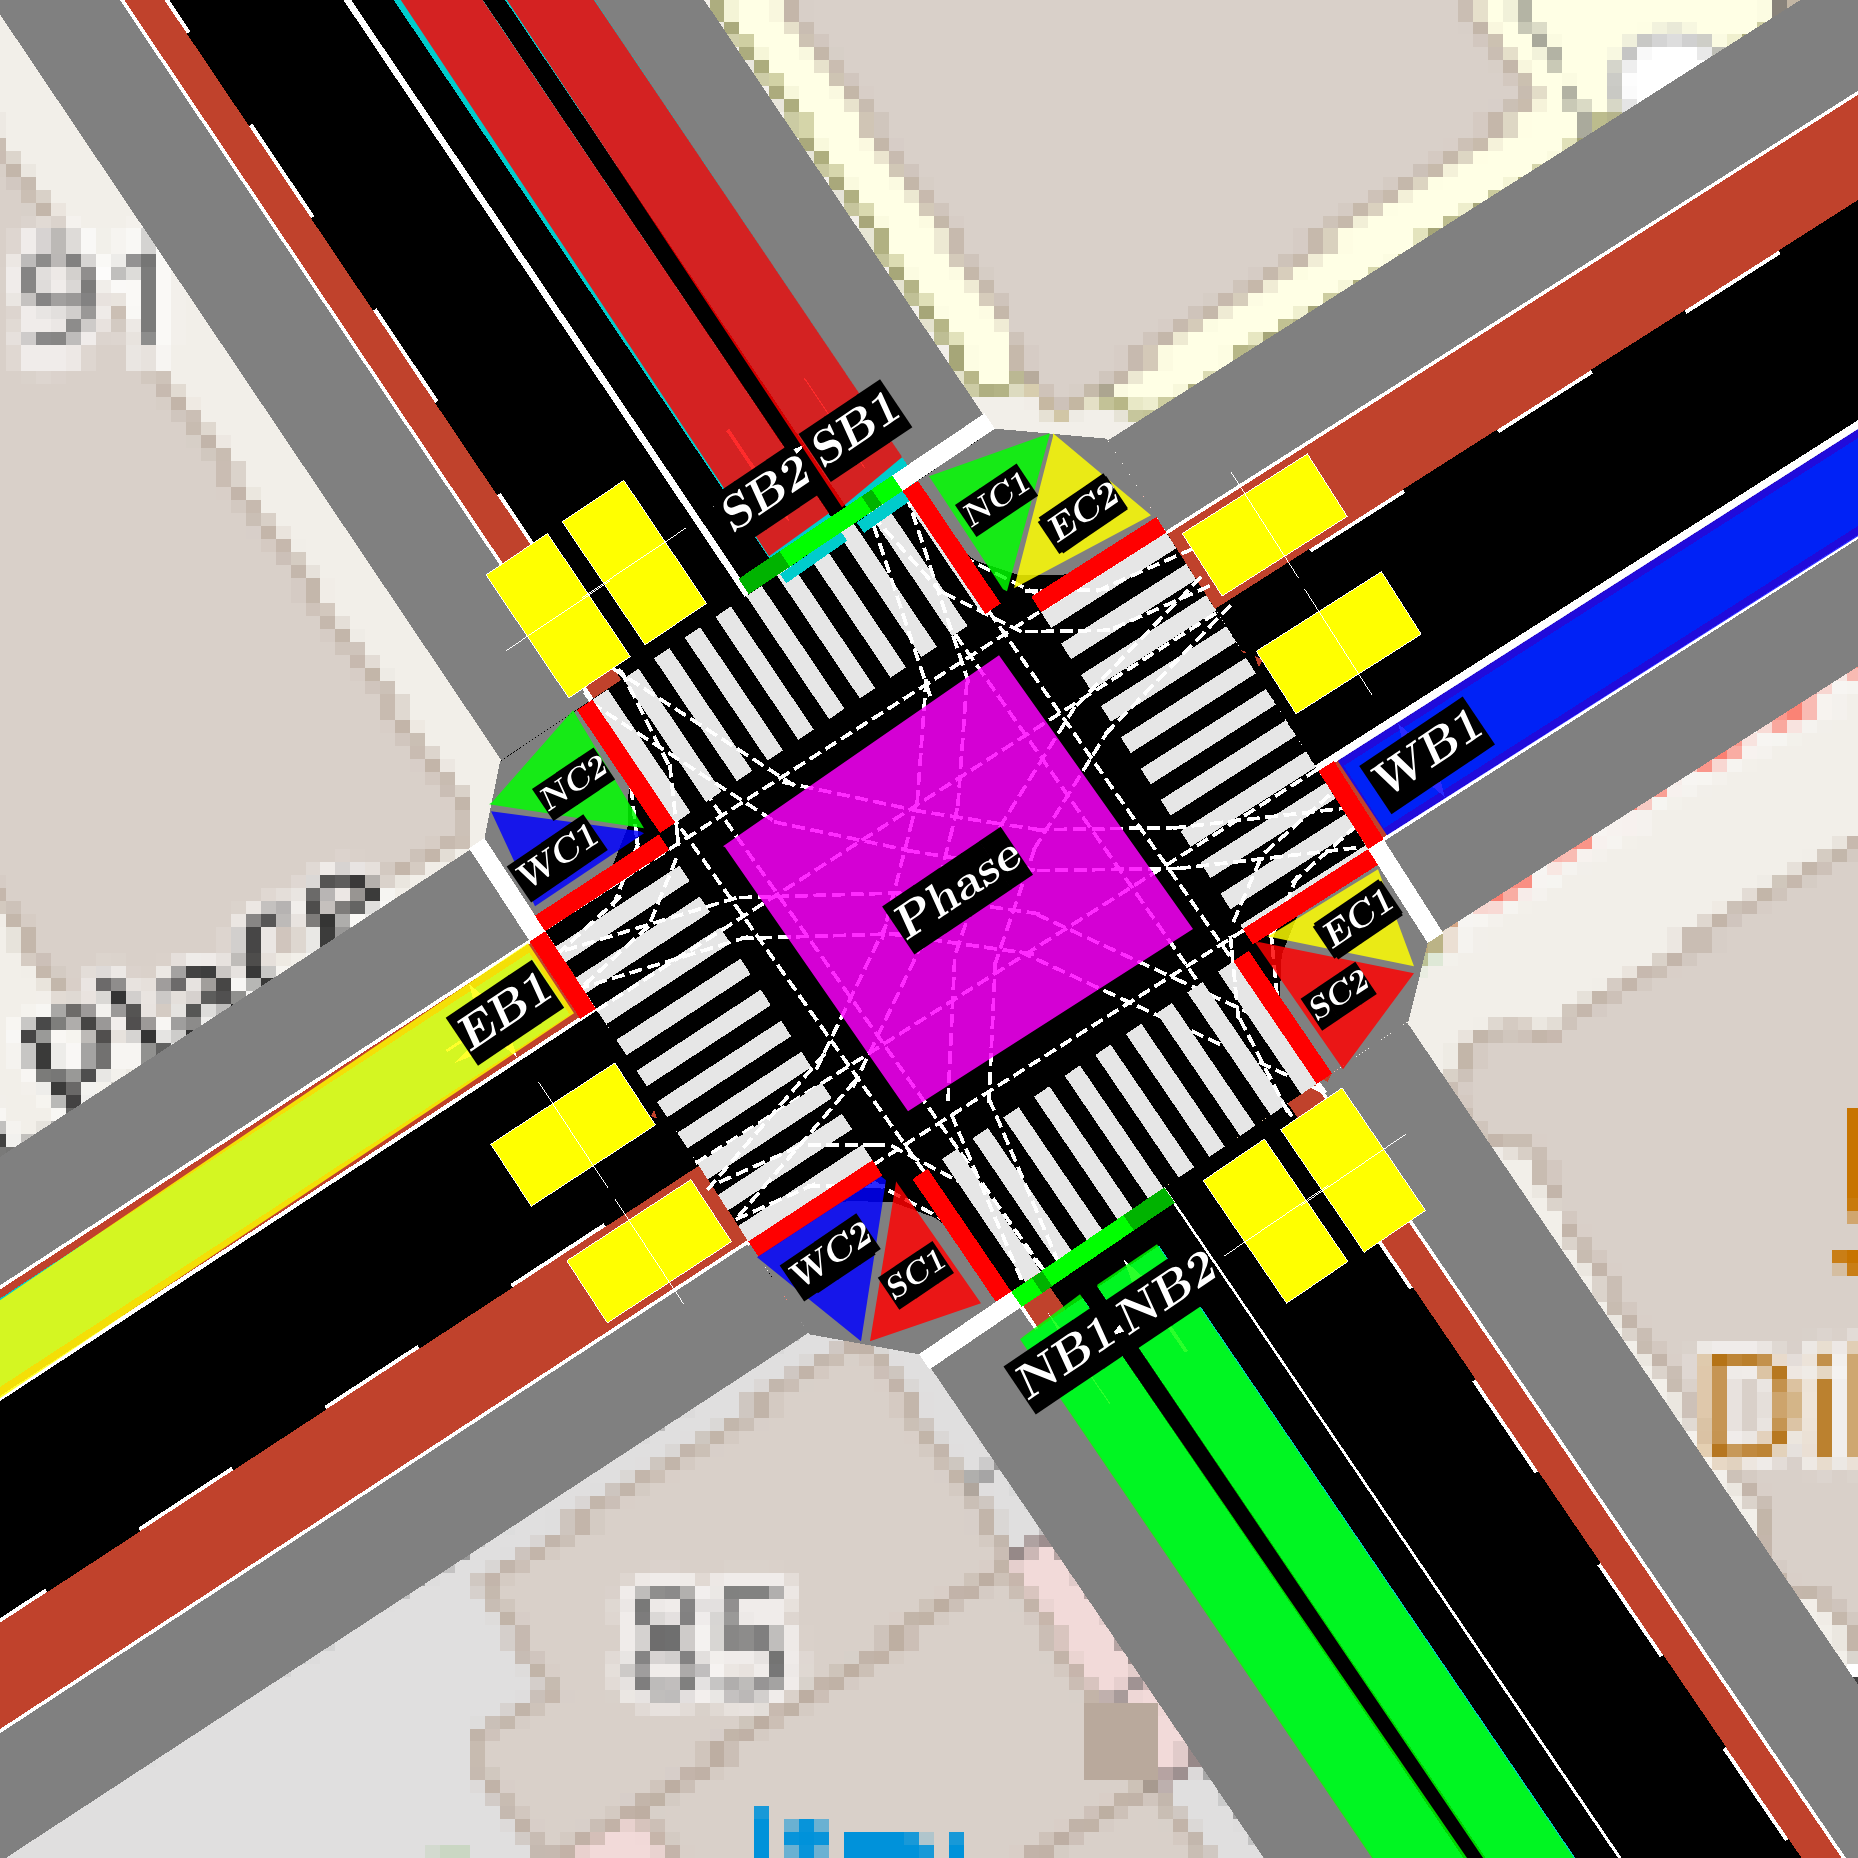
\includegraphics[width=\textwidth]{images/state_demo.png}
        \caption{TLS 1.}
    \end{subfigure}
    \hfill
    \begin{subfigure}{0.30\textwidth}
        \centering
        
\includegraphics[width=\textwidth]{images/state_crossing.png}
        \caption{TLS 2.}
    \end{subfigure}
    \hfill
    \begin{subfigure}{0.30\textwidth}
        \centering
        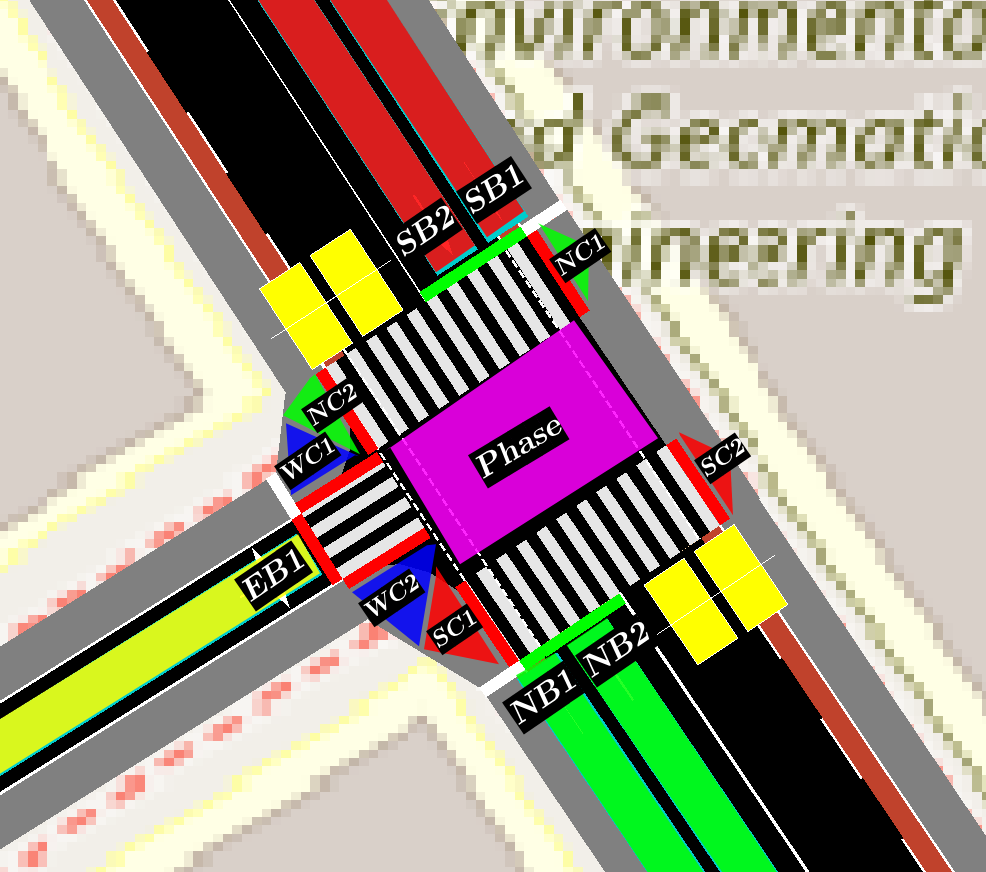
\includegraphics[width=\textwidth]{images/state_extended.png}
        \caption{TLS 3.}
    \end{subfigure}
    \caption{Annotated states in the extended network.}
    \label{fig:state_extended}
\end{figure}

Each of the three TLS have an action space of the same 3 actions, since each have lane approaches that can be divided into \emph{northbound}/\emph{southbound} and \emph{eastbound}/\emph{westbound}, which is the same as what defined in Table~\ref{tab:phase_actions}. The route generation parameters also remain exactly as before for training.

The set of neighbours $\mathcal{N}$ is defined for each TLS as follows:

\begin{table}[H]
  \centering
  \begin{tabular}{l | l}
    \textbf{Agent} & \textbf{Neighbours $\mathcal{N}$} \\
    \hline
    TLS 1 & $\{TLS_1, TLS_2\}$ \\
    TLS 2 & $\{TLS_1\}$ \\
    TLS 3 & $\{TLS_2\}$ \\
  \end{tabular}
  \caption{Set of neighbours for each traffic light system in the extended network.}
  \label{tab:extended_neighbours}
\end{table}

\begin{figure}[H]
    \centering
    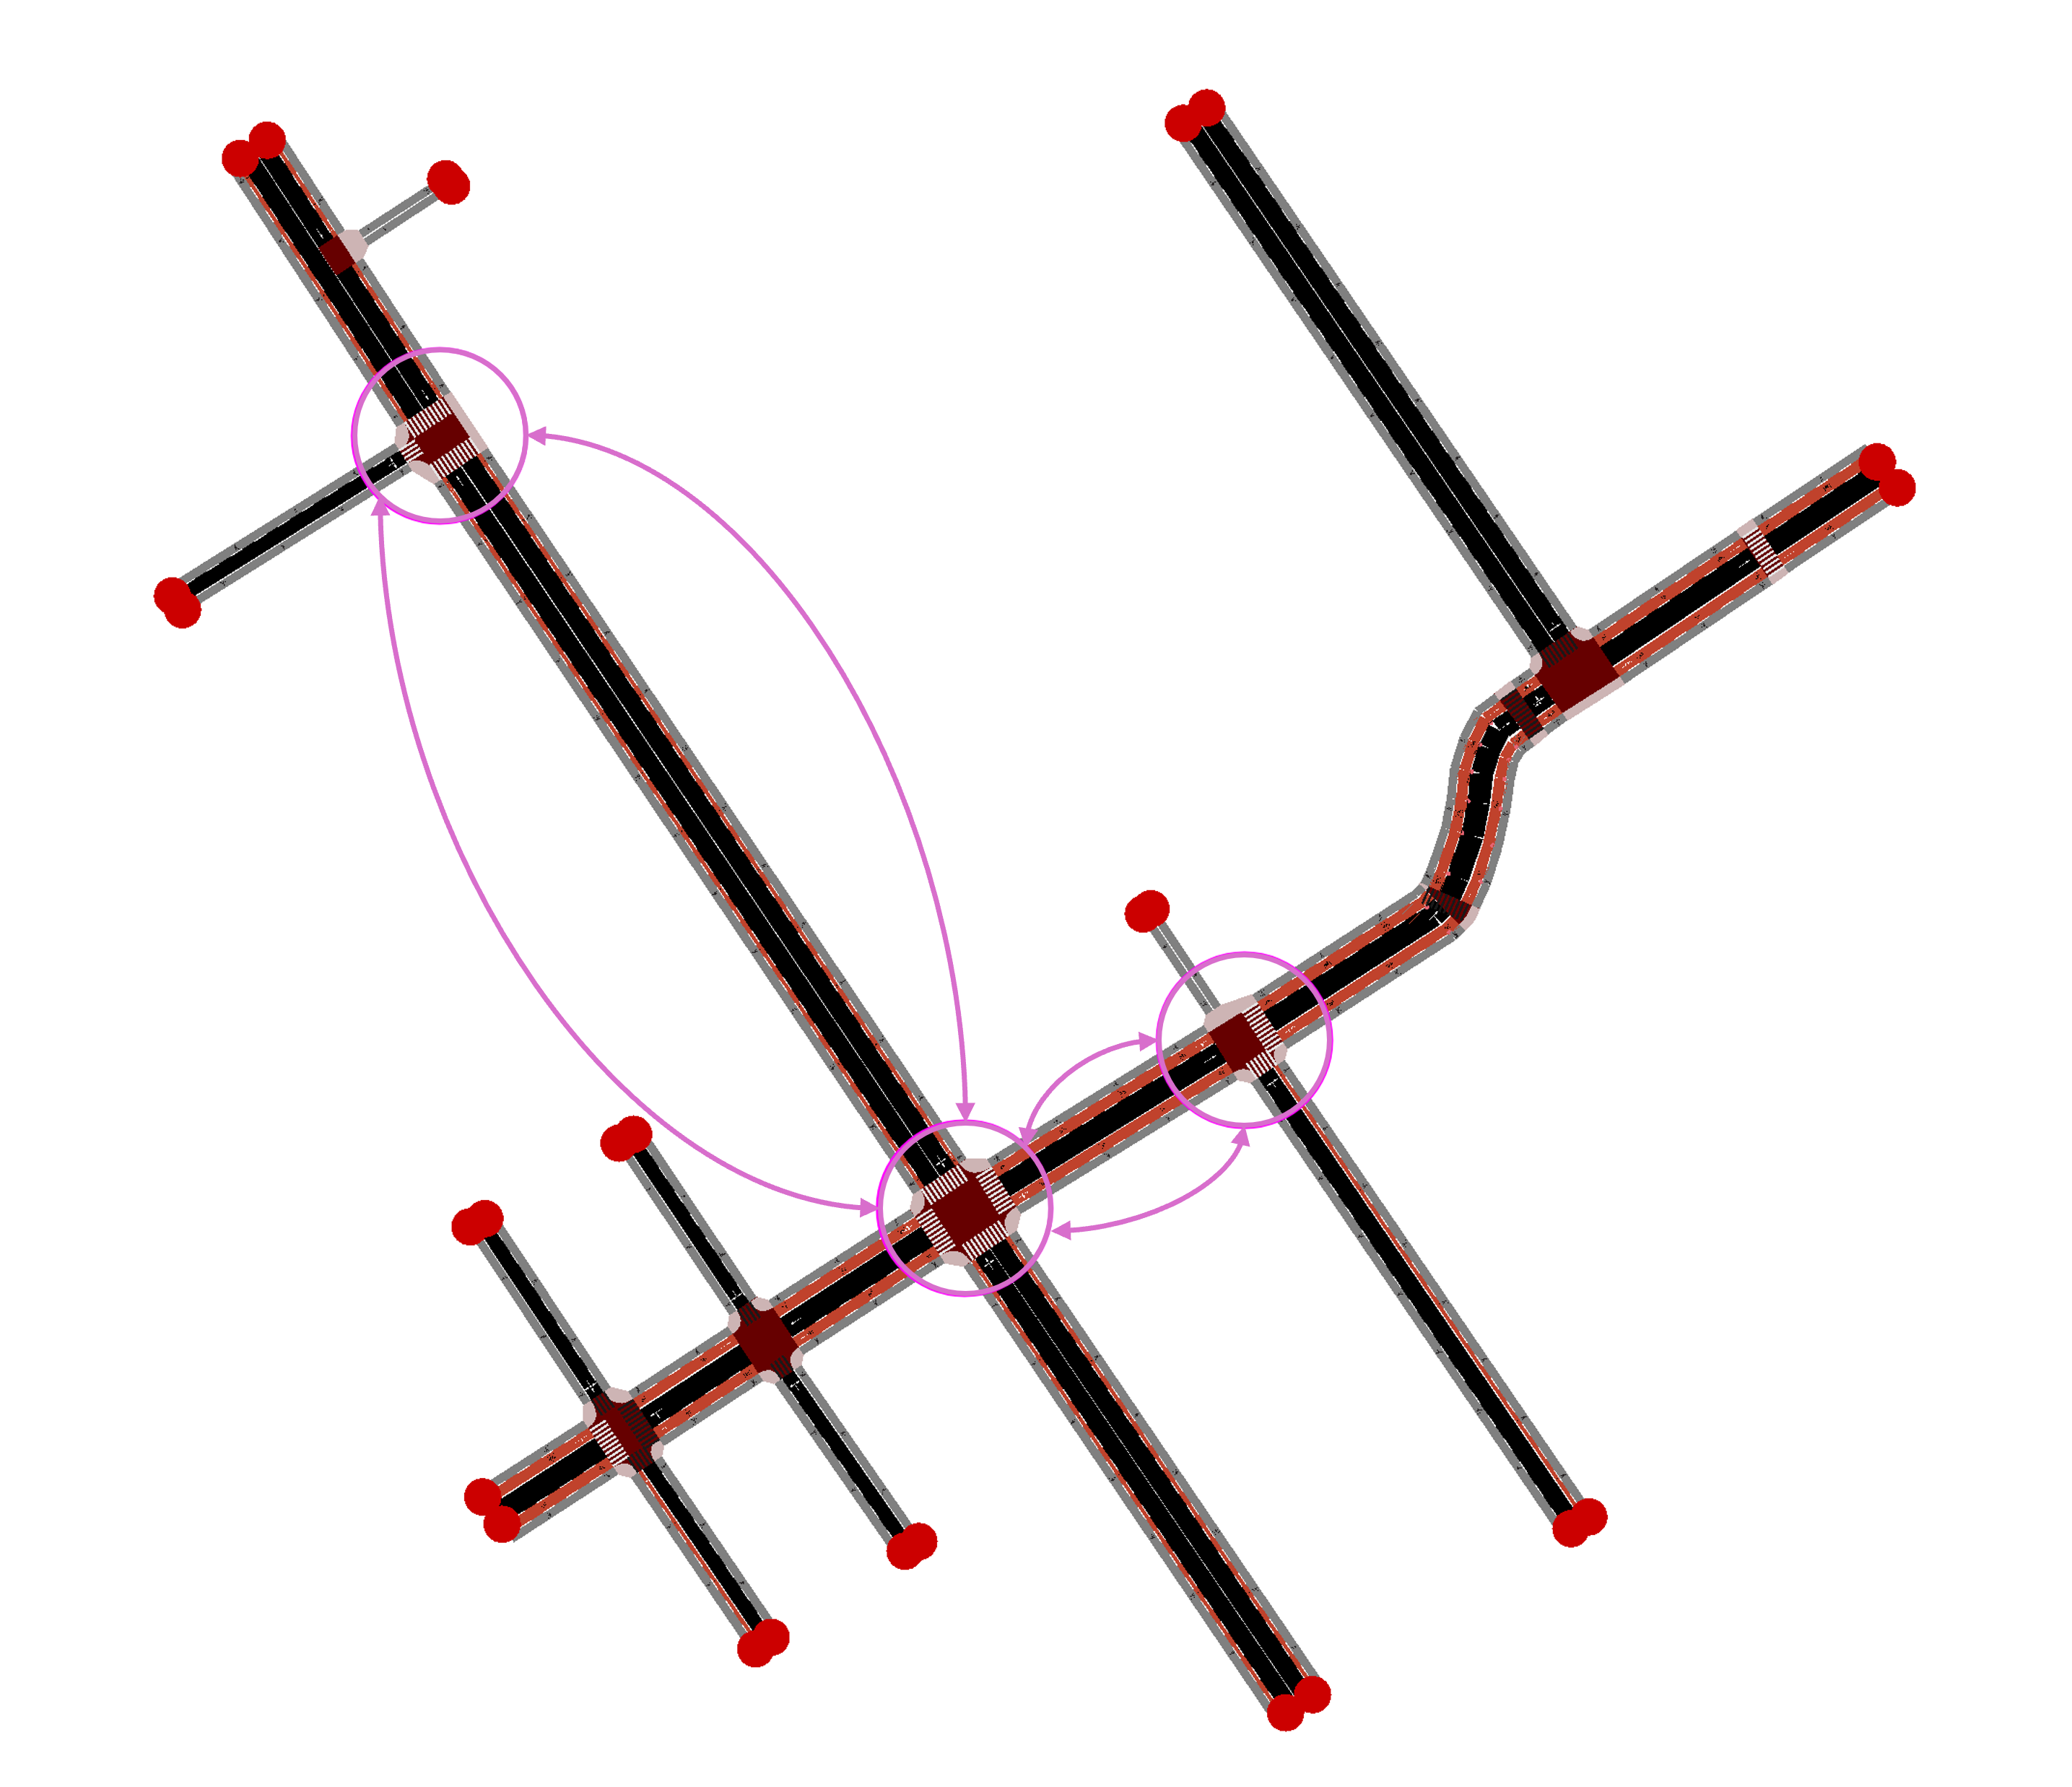
\includegraphics[width=0.64\textwidth]{images/extended_neighbours.png}
    \caption{Connection of traffic lights in the extended network.}
    \label{fig:extended_neighbours}
\end{figure}

\section{Results}

\subsection{System Requirements}

The Communicative Deep Q-learning algorithm was implemented as an extension to Deep Q-learning, utilising the same exact libraries. Implementing the network layer and communication bus only required the Python standard library. Training was also optimised to use the NVIDIA GeForce RTX 4070 Ti GPU, utilising CUDA, as before.

\subsection{Training}

We will train the three agents using the previous Deep Q-learning algorithm and -- in a separate training instance -- the Communicative Deep Q-learning algorithm. The three agents are trained together in the extended network using $10\,000$ generated traffic routes this time which follow the baseline traffic parameters. Each training episode has a duration of $3\,600$ steps.

As shown below, Deep Q-learning and Communicative Deep Q-learning perform significantly better than standard fixed-time control, both reaching a reward of \textgreater $8\,000$ units, compared to $1\,000$ units of the latter. Looking closer, Deep Q-learning reaches a final training reward of $\sim9\,000$ whereas Communicative Deep Q-learning reaches $\sim8\,000$.

\begin{figure}[H]
  \centering
  \begin{tikzpicture}
  \begin{axis}[
      width=14cm,
      height=8cm,
      xlabel={Epoch},
      ylabel={Reward},
      title={Extended network reward per epoch},
      grid=both,
      legend pos=south east
  ]

  \addplot[
      blue,
      mark=none
  ] table[
      x expr=\coordindex+1,
      y index=0
  ] {data/extended_train_ft.txt};
  \addlegendentry{Fixed-time control}

  \addplot[
      orange,
      mark=none
  ] table[
      x expr=\coordindex+1,
      y index=0
  ] {data/extended_train_dqn_c0.txt};
  \addlegendentry{Deep Q-learning}

  \addplot[
      magenta,
      mark=none
  ] table[
      x expr=\coordindex+1,
      y index=0
  ] {data/extended_train_cdqn_c0.txt};
  \addlegendentry{Comm. Deep Q-learning}

  \end{axis}
  \end{tikzpicture}
  \caption{Reward per training route in the extended environment (runtime: 13:41:12).}
  \label{fig:communicative_deep_q_learning_extended_train}
\end{figure}

We see that the rewards between the two are about equivalent up until epoch $\sim600$ where the two algorithms begin to diverge slightly. Although we expect Communicative Deep Q-learning to perform at least as well, if not better, than Deep Q-learning, this may be attributed to it having a much larger input state for each of the agents' neural networks. Therefore, it would require a longer training period to reach the same given reward.

The spikes observed are the penalties we discussed previously, and are an artefact of the SUMO simulation software -- not the algorithms themselves.

\subsection{Evaluation}

Now we evaluate the sets of Deep Q-learning agents and Communicative Deep Q-learning agents using the evaluation configurations defined previously in Table~\ref{tab:evaluation_configs}. After generating the 100 evaluation scenarios, and taking the median values, we get the following results.

For each scenario, the Deep Q-learning agents perform the best, followed by the Communicative Deep Q-learning agents, and then finally the fixed-time control TLS. The difference between the prior two is narrow, and we have conjectured that this is due to the training time not being as sufficient for Communicative Deep Q-learning since it has a larger neural network.

\begin{figure}[H]
  \centering
  \begin{tikzpicture}
  \begin{axis}[
      width=14cm,
      height=8cm,
      xlabel={Evaluation},
      ylabel={Reward},
      title={Extended network reward per evaluation scenario},
      grid=both,
      legend style={at={(0.03,0.5)},anchor=west},
      xtick=data
  ]

  \addplot[
      blue,
      mark=none
  ] table[
      x expr=\coordindex+1,
      y index=0
  ] {data/extended_eval_ft.txt};
  \addlegendentry{Fixed-time control}

  \addplot[
      orange,
      mark=none
  ] table[
      x expr=\coordindex+1,
      y index=0
  ] {data/extended_eval_dqn_c0.txt};
  \addlegendentry{Deep Q-learning}

  \addplot[
      magenta,
      mark=none
  ] table[
      x expr=\coordindex+1,
      y index=0
  ] {data/extended_eval_cdqn_c0.txt};
  \addlegendentry{Comm. Deep Q-learning}

  \end{axis}
  \end{tikzpicture}
  \caption{Median reward for evaluation routes in the extended environment.}
  \label{fig:communicative_deep_q_learning_extended_eval}
\end{figure}


Unexpectedly, it appears that Communicative Deep Q-learning has failed to make a meaningful improvement. Although our agents gain extra information, they do not necessarily make better decisions. This is due to one of the fundamental flaws of Q-learning itself that our actions are discrete with no way for our agent to adaptively adjust the timings based on adjacent states.

One possible extension is Parametrised Deep Q-Networks (PDQN) \cite{XiongWanYangEtAl2018} in which we could replace the internal DQN model whilst maintaining the Communicative infrastructure we have developed. PDQN enables our discrete actions -- switching traffic light phase -- to have a duration that is varied dynamically by the agent (e.g.\ the traffic light phase duration could be chosen from a continuous interval instead of being fixed at a single value). Thus enabling agents to carry out smarter, more flexible behaviour based on state communicated to them.

\subsection{Emergent Behaviour}

In our literature review, we noted that centralised systems such as SCOOT group signals into regions and make dynamic adjustments to improve coordination between traffic lights. This helps promote ``green waves'' where vehicles encounter consecutive green lights without having to stop.

Unlike these systems, our Communicative Deep Q-learning agents are decentralised. This has the benefit that hardware can be limited to the traffic light system itself without requiring a larger centralised system. The only connections it would need is to adjacent agents, enabling easy extensions.

Despite Communicative Deep Q-learning not performing better in the evaluation routes which tested traffic in all directions of varying congestion levels, we observe that it may learn to create green waves (which was \emph{not} explicitly programmed) which is not possible with standard Deep Q-learning agents.

Consider the synthetic traffic route in which a continuous flow of vehicles travel from A to B. We insert a new car into the simulation at an expected rate of $0.25$ / s following the Poisson distribution, and run the simulation for $3\,600$ steps.

\begin{figure}[H]
    \centering
    \includegraphics[width=0.48\textwidth]{images/green_wave_route.png}
    \caption{Single traffic route from A to B.}
    \label{fig:green_wave_route}
\end{figure}

Our Communicative Deep Q-learning agents learn to synchronise the lights such that the vehicles continue to pass through with minimal disruption. The Deep Q-learning agents were unable to do the same, leading to occasional congestion, reducing overall reward.

\begin{figure}[H]
    \centering
    \begin{subfigure}{0.48\textwidth}
        \centering
        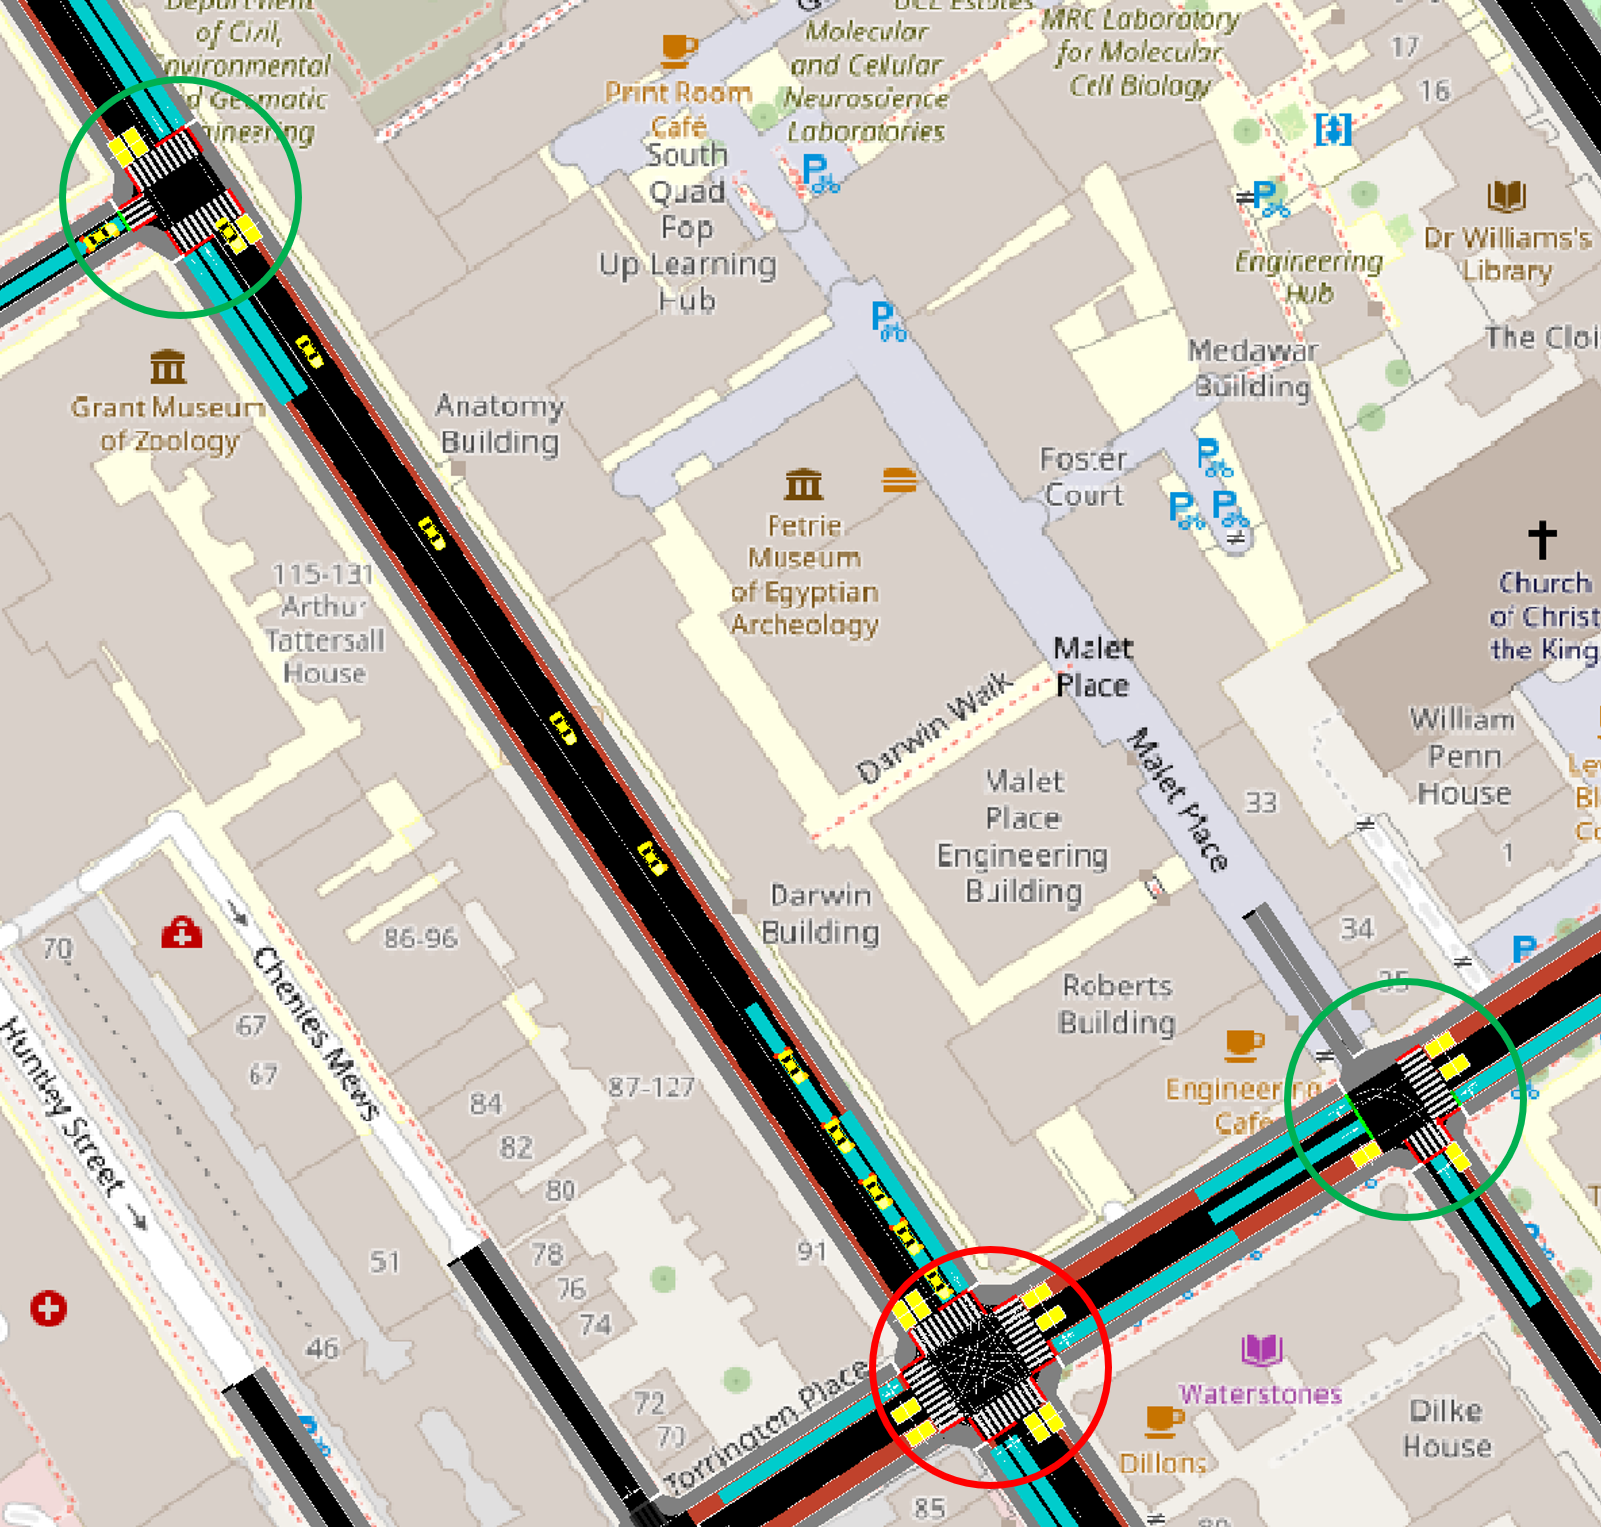
\includegraphics[width=\textwidth]{images/green_wave_dqn.png}
        \caption{Congestion with Deep Q-learning\\(reward: $19\,725$).}
        \label{fig:green_wave_dqn}
    \end{subfigure}
    \hfill
    \begin{subfigure}{0.48\textwidth}
        \centering
        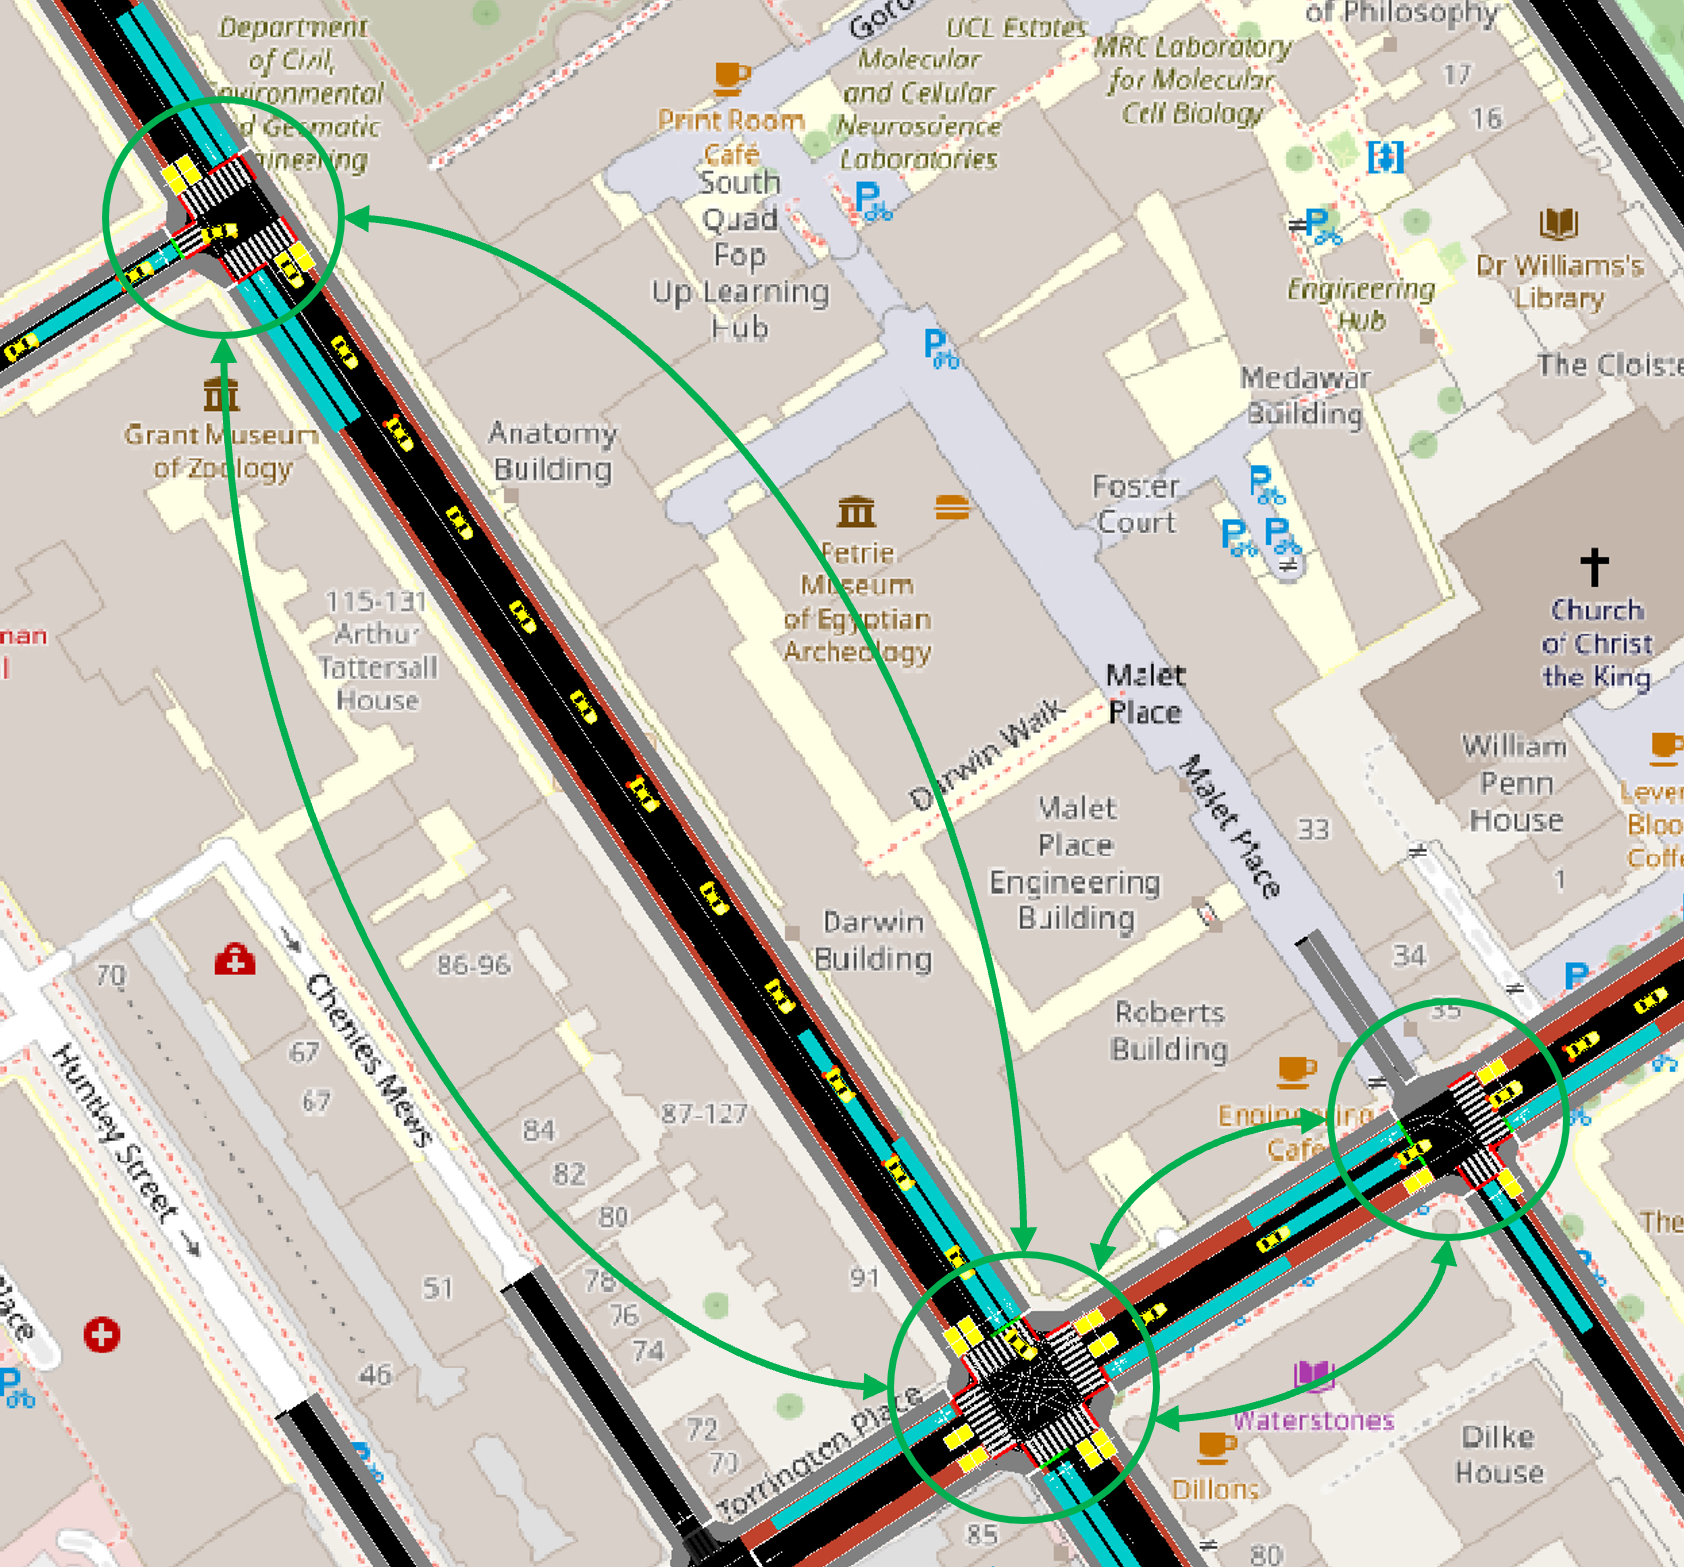
\includegraphics[width=\textwidth]{images/green_wave_cdqn.png}
        \caption{Green wave with Comm. Deep Q-learning\\(reward: $21\,006$).}
        \label{fig:green_wave_cdqn}
    \end{subfigure}
    \caption{Example of learnt green wave behaviour via communication.}
    \label{fig:green_wave_simulation}
\end{figure}

\section{Summary}

This chapter explored the motivation for implementing Communicative Deep Q-learning, and the novel features we added to enable communication between the agents. In addition, we developed a new extended network consisting of multiple traffic lights, to enable a multi-agent system.

Finally, we trained and compared Deep Q-learning agents to Communicative Deep Q-learning agents in a diverse set of scenarios. We conclude that whilst a communication bus provides agents with more information, and may lead to additional emergent behaviours, the internal DQN architecture bottlenecks what can be done with the communication abilities.

\chapter{Conclusions} \label{chapter:conclusions}

\section{Achievements}

After a comprehensive review of existing traffic light systems, we conclude that there are fundamental limitations; today's systems rely on predefined logic which may fail to perform optimally in all conditions and there is no capability for \emph{self-learning}. Thus, we motivate the need for intelligent agents which use reinforcement learning.

Three detailed simulated environments where traffic experiments could be conducted were created, respectively dubbed `demo', `crossing', and `extended'. Through the use of open source tools provided by the traffic simulation package SUMO, real world locations could be virtualised into abstracted computer representations with synthesised traffic of varying conditions.

Finally, we incrementally built three algorithms de novo, justifying each along the way: Q-learning, Deep Q-learning, and Communicative Deep Q-learning. For our purposes, Q-learning was not sufficient for the state space was too large. Deep Q-learning introduced neural networks that serve as powerful approximation machines. We then built a novel Communicative Deep Q-learning algorithm, which allowed for the decentralised agents to confer local state.

\section{Evaluation}

In Chapter~\ref{chapter:introduction}, it was stated the overall aim of this dissertation was to perform a detailed analysis and evaluation of how an intelligent agent may be used to hopefully improve upon existing traffic light systems. The three objectives that were defined -- which we bifurcate even further -- are as follows:

\paragraph{1. Construct an environment in which our experiments will be conducted.}

Firstly, we (a) defined the boundaries of the environment using the OpenStreetMap software, which was namely University College London's Bloomsbury Campus.

Following this, we (b) researched tools which could be used for traffic simulation. We decided on the SUMO, an open source package which allows for creation of a traffic network as well as traffic generation.

Finally, (c) three distinct environments were manually built using SUMO, with attention to detail with regards to things such as lane and junction priorities.

\paragraph{2. Develop our own intelligent agents in a progressive manner.}

In the literature review, (a) existing traffic light systems were analysed in detail, including their inherit limitations -- why intelligent agents are needed in the first place.

From first principles the (b) foundations of intelligent agents, namely the Markov Decision Process, was explored in an intuitive manner. The states and actions were also clearly defined. 

Afterwards, (c) the three algorithms themselves were developed in a way which was (d) incremental with explicit justifications along the way. 

\paragraph{3. Evaluate the intelligent agents in the simulated environment.}

For our intelligent agents, (a) training and evaluation was completed in a diverse set of scenarios that had varying road structure and traffic conditions.

Specifically, (b) the evaluation made use of a reward calculated from a weighted formula which took into account the impact on both pedestrians and vehicles -- considered equally.

The last sub-objective was to (c) assess the feasibility of our agents in reality, which we have not yet done in a clear manner, but we will do below. Our agents require a way to receive state, choose an action, and communicate with other agents in the case of Communicative Deep Q-Learning.

\subsection{Feasibility of Intelligent Agents}

Cameras could be installed which serve as lane area detectors. A computer vision algorithm could perhaps be run to count how many cars there are in an image. For pedestrians, infrared sensors could be added to detect and count their presence.

In the case of Deep Q-Learning we run a neural networks. Given the architecture is small, it won't require very powerful hardware for inferencing. In fact, it could be reasonably run on a consumer grade CPU, though one would be needed per traffic light system.

Local communication channels between adjacent agents are needed to share state -- perhaps underground copper cables. At a city scale this would likely be cheaper than current centralised systems that would otherwise require lengthy connections to a central computer.

Based on our `back-of-the-envelope' analysis, intelligent agents are feasible in practice. Care must be taken to ensure the agent models installed onto traffic light controllers are trained extensively and sufficiently (in simulation), since a poor action policy may have terrible consequences.

\section{Future Work}

Although we have successfully met \emph{all} objectives we initially set out to complete, there remains a few areas of refinement for the project. Furthermore, we will discuss interesting directions in which the project could be continued, building upon the foundations laid by this dissertation.

\subsection{Simulated Environment} 

Per the Cambridge Dictionary, a simulation is defined as ``a \emph{model} of a real activity''. As with all models, there are inconsistencies between it and the real deal, and our built environment is no exception.

Firstly, based on observations it appears that cars and pedestrians are more risk prone compared to real life. Their behaviour shows little to no hesitation, acting with perfect reaction times. Human emotions that influence actions (e.g.\ being annoyed) are abstracted away, making the entities more predictable or `deterministic'.

The traffic parameter \texttt{--fringe-factor} was set to Max meaning vehicles only spawn from the very edges, and each edge was given an equal weighting leading to no notion of more/less commonly used roads. Therefore behaviour such as starting from a parking area in the middle of the road is not accounted for, nor is the act of pedestrians going into or out of buildings.

Lastly, ideally, the network would be scaled to be much, much larger than what it currently is to examine the cumulative effects of intelligent agents. Alas, this was not possible due to the resource constraints of the project, given the process of creating an environment replica is laborious. 

\subsection{Reinforcement Learning Algorithms} 

Our set of algorithms concluded with Communicative Deep Q-Learning in which a limitation was unveiled. Specifically, our defined actions were discrete with no way for the agent to adaptively adjust the timings.

We proposed an extension that would replace the current Deep Q-Network (DQN) with a Parameterised version to enable dynamic timings. This would hopefully allow for better use of the communication abilities. Increasing the state information to include the current phase duration would be desirable as well. 

In addition to Parameterised DQN, there exists a breadth of adjacent Q-learning variants including Double DQN or Dueling DQN. There is even a class of algorithms that follow an entirely different methodology known as Actor-Critic.

Reinforcement learning algorithms do not provide the same guarantees as fixed-time control. To give an example, our agents as they are may find themselves in a scenario where if there is dominant non-stop flow of traffic in one direction, and a single vehicle waiting to go in an orthogonal direction, the latter may be starved indefinitely. Therefore care should be taken (i.e.\ additional measures added) to avoid these scenarios.

\section{Closing Remarks}

After what has been a lengthy journey we reach the eucatastrophe. Close to $\sim50$ distinct training and evaluation results have been gathered\footnotemark\footnotetext{Excluding the \emph{many} that had to be repeated!} in which there has been a cumulative training time of over 100 hours, with some experiments even spanning multiple nights in a row.

Hopefully this dissertation has given insight into how decentralised intelligent agents may be used to save time for both vehicles and pedestrians, taking existing traffic light systems a step further.

\appendix

\begin{thebibliography}{HHM99}

\bibitem[Tha17]{ThamesLeisureFacts2017}
Thames Leisure.
\newblock 12 amazing facts about London.
\newblock {\em Thames Leisure}, archived January 7, 2017.
\newblock Available at:
  https://web.archive.org/web/20170107005431/http://www.thamesleisure.co.uk/12-amazing-facts-london/.

\bibitem[ASC17]{FHWA_ASCT17}
Federal Highway Administration.
\newblock EDC-1: Adaptive Signal Control Technology.
\newblock {\em Federal Highway Administration}, 2017.
\newblock Available at:
  https://www.fhwa.dot.gov/innovation/everydaycounts/edc-1/asct.cfm.

\bibitem[ITSS20]{ITSS2020}
Intelligent Transportation Systems Society, Pennsylvania State University.
\newblock Reinforcement Learning for Traffic Signal Control.
\newblock {\em Intelligent Transportation Systems Society, Pennsylvania State University}, September 20, 2020.
\newblock Available at:
  https://traffic-signal-control.github.io/.

\bibitem[HW08]{HaklayWeberOSM08}
M.~Haklay and P.~Weber.
\newblock OpenStreetMap: User-generated street maps.
\newblock {\em IEEE Pervasive Computing}, 7(4): 12--18, 2008.
\newblock doi:10.1109/MPRV.2008.80.

\bibitem[HWC]{HighwayCode159to203}
Department for Transport.
\newblock The Highway Code: Using the road (Rules 159--203).
\newblock {\em GOV.UK}.
\newblock Available at:
  https://www.gov.uk/guidance/the-highway-code/using-the-road-159-to-203.

\bibitem[GS55]{GerloughSchuhl1955}
D.~L.~Gerlough and A.~Schuhl.
\newblock Use of Poisson Distribution in Highway Traffic: The Probability Theory Applied to Distribution of Vehicles on Two-Lane Highways.
\newblock {\em Research Paper, Eno Foundation for Highway Traffic Control}, 1955.
\newblock Available at:
  https://rosap.ntl.bts.gov/view/dot/16299.

\bibitem[GBG]{GoelBusGershenson}
S.~Goel, S.~F.~Bus and C.~Gershenson.
\newblock Self-Organisation in Traffic Lights: Evolution of Signal Control with Advances in Sensors and Communications.
\newblock {\em Research Paper, University at Albany}.
\newblock Available at:
  https://arxiv.org/pdf/1708.07188.

\bibitem[DfT23]{PedestrianCrossings23}
Department for Transport.
\newblock Know your traffic signs: Pedestrian, cycle and equestrian crossings.
\newblock {\em GOV.UK}, 5 December 2023.
\newblock Available at:
  https://www.gov.uk/government/publications/know-your-traffic-signs/pedestrian-cycle-and-equestrian-crossings.

\bibitem[Li23]{LiPengHouEtAl2023}
J.~Li, L.~Peng, K.~Hou, Y.~Tian, Y.~Ma, S.~Xu and T.~Z.~Qiu.
\newblock Adaptive signal control and coordination for urban traffic control in a connected vehicle environment: A review.
\newblock {\em Digital Transportation and Safety}, 2(2): 89--111, 2023.
\newblock doi:10.48130/DTS-2023-0008.
\newblock Available at:
  https://maxapress.com/article/doi/10.48130/DTS-2023-0008.

\bibitem[ITS12]{ITS2012}
Institute for Transport Studies, University of Leeds.
\newblock Urban traffic control systems: Evidence on performance.
\newblock {\em Institute for Transport Studies, University of Leeds}, archived October 19, 2012.
\newblock Available at:
  https://web.archive.org/web/20121019152217/
  http://www.konsult.leeds.ac.uk/private/level2/instruments/instrument014/l2\_014c.htm.

\bibitem[CU21]{CesmeUrbanikII2021}
B.~Cesme and T.~Urbanik~II.
\newblock Signal Coordination: Are We Really Coordinating For All Users?
\newblock {\em Kittelson \& Associates, Inc.}, October 15, 2021.
\newblock Available at:
  https://www.kittelson.com/ideas/pros-and-cons-of-signal-coordination/.

\bibitem[SIIG04]{FHWA_SIIG04}
Federal Highway Administration.
\newblock Signalized Intersections: Informational Guide — Chapter 9: Intersection-Wide Treatments.
\newblock {\em Federal Highway Administration}, August, 2004.
\newblock Available at:
  https://www.fhwa.dot.gov/publications/research/safety/04091/09.cfm.

\bibitem[PS64]{Stewart1964}
P.~Stewart.
\newblock "I know it when I see it".
\newblock {\em Jacobellis v. Ohio}, 1964.
\newblock Available at:
  https://en.wikipedia.org/wiki/I\_know\_it\_when\_I\_see\_it.

\bibitem[Tr26]{TraCIProtocol26}
German Aerospace Center (DLR).
\newblock TraCI Protocol Specification.
\newblock {\em SUMO Documentation}, February 13, 2026.
\newblock Available at:
  https://sumo.dlr.de/docs/TraCI/Protocol.html.

\bibitem[Sta19]{StatistaCarOccupancy}
Statista Research Department.
\newblock Average car and van occupancy in England from 2002 to 2018.
\newblock {\em Statista}, July, 2019.
\newblock Available at:
  https://www.statista.com/statistics/314719/average-car-and-van-occupancy-in-england/.

\bibitem[RS90]{RichardSutton1990}
R.~S.~Sutton. and M.~L.~Littman.
\newblock The reward hypothesis.
\newblock {\em Web page, University of Alberta}, ~1990.
\newblock Available at:
  http://incompleteideas.net/rlai.cs.ualberta.ca/RLAI/rewardhypothesis.html.

\bibitem[DGC]{DemosGraphingCalculator}
Desmos Studio.
\newblock Graphing Calculator.
\newblock {\em Desmos}, 2011.
\newblock Available at:
  https://www.desmos.com/calculator.

\bibitem[Mi18]{MismarChoiEvans2018}
F.~B.~Mismar, J.~Choi and B.~L.~Evans.
\newblock A framework for automated cellular network tuning with reinforcement learning.
\newblock {\em arXiv preprint arXiv:1808.05140}, 2018.
\newblock doi:10.48550/arXiv.1808.05140.
\newblock Available at:
  https://arxiv.org/abs/1808.05140.

\bibitem[SLi23]{SLi2023}
S.~E.~Li.
\newblock Reinforcement Learning for Sequential Decision and Optimal Control.
\newblock {\em First ed., Springer Verlag, Singapore}, 1--460, 2023.
\newblock doi:10.1007/978-981-19-7784-8.

\bibitem[ATE25]{ActiveTravel25}
Active Travel England.
\newblock Critical safety issues for walking, wheeling and cycling.
\newblock {\em GOV.UK}, 6 November 2025.
\newblock Available at:
  https://www.gov.uk/government/publications/critical-safety-issues-for-walking-wheeling-and-cycling/critical-safety-issues-for-walking-wheeling-and-cycling.

\bibitem[JXi18]{XiongWanYangEtAl2018}
J.~Xiong, Q.~Wang, Z.~Yang, P.~Sun, L.~Han, Y.~Zheng, H.~Fu, T.~Zhang, J.~Liu, H.~Liu.
\newblock Parametrized Deep Q-Networks Learning: Reinforcement Learning with Discrete-Continuous Hybrid Action Space.
\newblock {\em arXiv preprint arXiv:1810.06394}, 2018.
\newblock doi:10.48550/arXiv.1810.06394.
\newblock Available at:
  https://arxiv.org/abs/1810.06394.

\end{thebibliography}

\chapter{Supplementary Analysis}

\section{State Compression}

As discussed in Section~\ref{q_learning_training}, the uncompressed state representation from Formula~\ref{state_formula} leads to a combinatorially large state space, rendering the standard tabular Q-learning ineffective. We addressed this by developing the Deep Q-learning algorithm, which utilises neural networks to estimate the optimal quality function $Q^*$.

This proved to be very effective, but could we find a way to make the standard Q-learning algorithm still work? One way that was experimented with was a series of \emph{state compression} strategies that reduce the dimensionality of the state tuple, without completely removing all information.

Three compression levels are defined, denoted as $\texttt{C0}$, $\texttt{C1}$, and $\texttt{C2}$, where $\texttt{C0}$ corresponds to the original uncompressed representation, and higher levels apply increasingly aggressive compression on the state.

\subsection{Compression Levels}

We will use the original demo network again as an example to illustrate the compression levels. Recall the notation defined in Section~\ref{q_learning_state} that we use for the vehicle lanes and pedestrian waiting areas in the annotated state diagram below.

\begin{figure}[H]
    \centering
    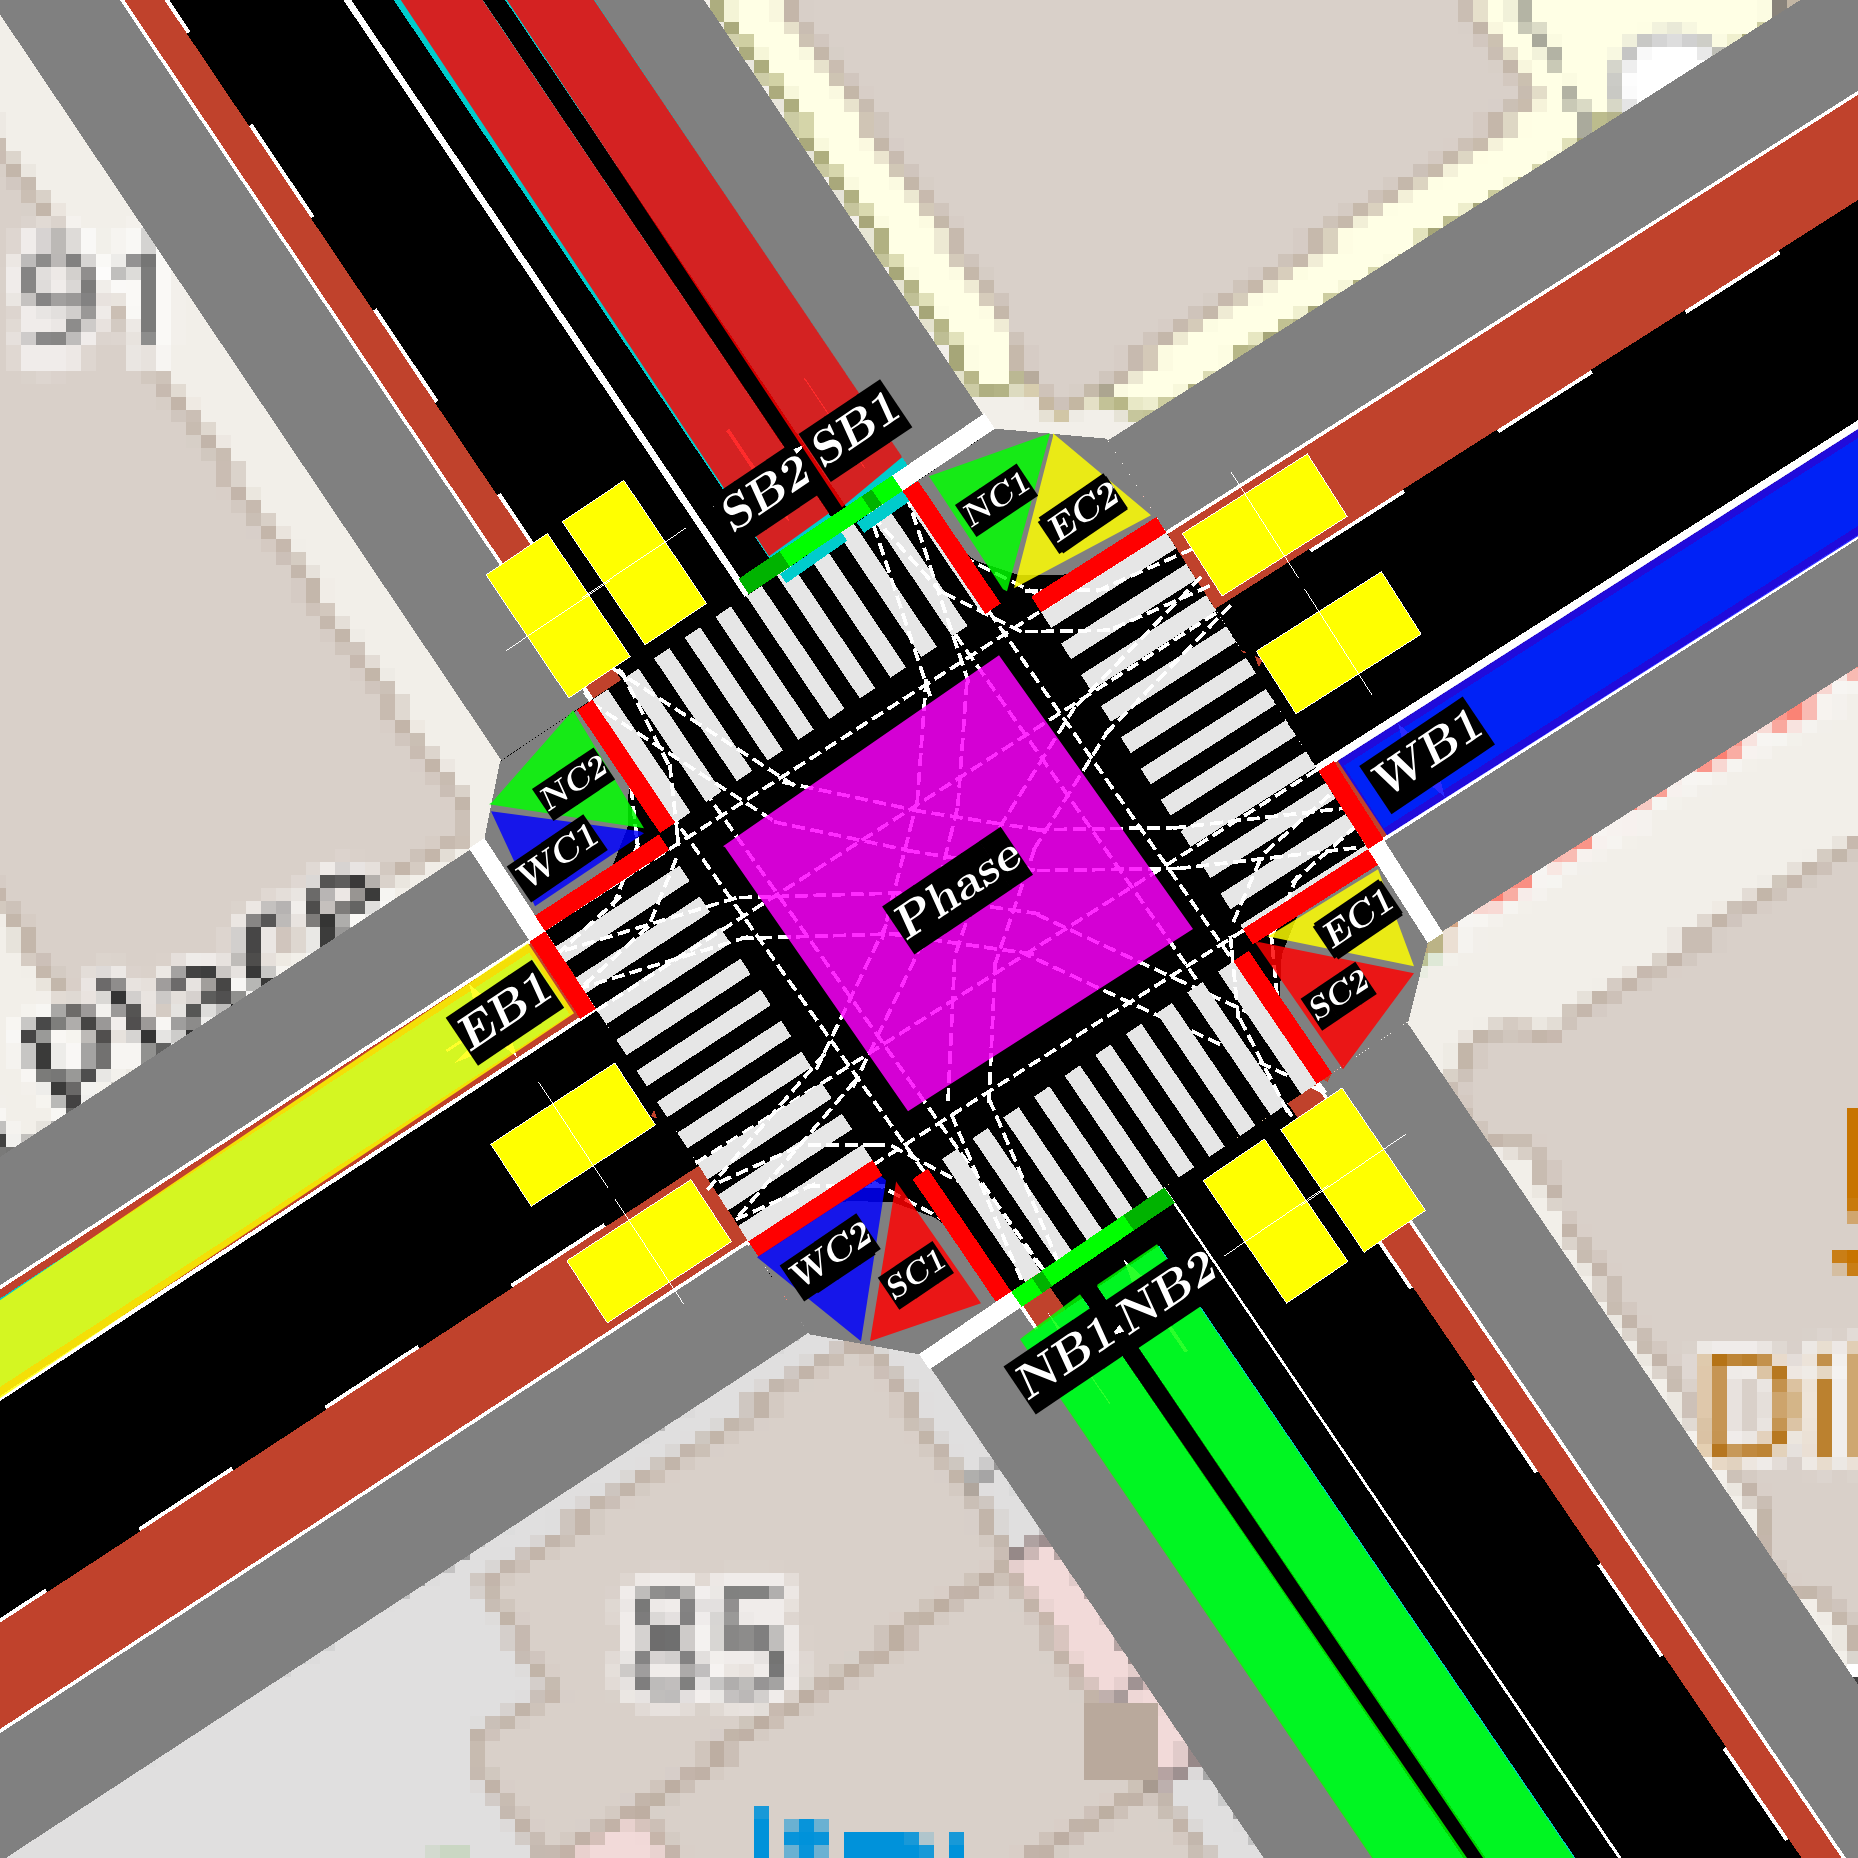
\includegraphics[width=0.48\textwidth]{images/state_demo.png}
    \caption{Annotated state in the demo network.}
\end{figure}

\paragraph{C0: Uncompressed State}

This corresponds to the original state we obtain using the Formula~\ref{state_formula}. Each vehicle lane and pedestrian waiting area (split based on direction) is represented individually:

\[
  Veh_t = (NB_1, NB_2, WB_1, SB_1, SB_2, EB_1)
\]
\[
  Ped_t = (SC_1, SC_2, WC_1, WC_2, NC_1, NC_2, EC_1, EC_2)
\]
\begin{equation}
  S_t = (Phase_t,) + Veh_t + Ped_t
\end{equation}

From this, we see that the demo traffic light system can be encoded as a 15-tuple. This is highly expressive, but it leads to an excessively large state space for Q-learning to be effective as calculated previously in Section~\ref{q_learning_training} ($\sim 9\times10^{12}$ states).

\paragraph{C1: Directional Aggregation}

At the first level of compression, we aggregate values within each directional group. Specifically:

\begin{itemize}
  \item All vehicle lanes belonging to the same approach are summed (e.g.\ northbound approaches, $NB_1$ + $NB_2$ $\rightarrow$ $NB$).
  \item All pedestrian waiting areas associated with the same crossing are summed (e.g.\ west crossings, $WC_1$ + $WC_2$ $\rightarrow$ $WC$).
\end{itemize}

This reduces the dimensionality of the state by collapsing per-lane and per-wait-area information respectively. Formally, the sate now becomes:

\[
  Veh_t = (NB, WB, SB, EB)
\]
\[
  Ped_t = (SC, WC, NC, EC)
\]
\begin{equation}
  S_t^{(C1)} = (Phase_t,) + Veh_t + Ped_t
\end{equation}

Our state tuple $S$ now consists of 9 parts. Recall in Section~\ref{q_learning_training} where we said there were 3 possible traffic light phases, each vehicle detector had a count in range 0--8 on average, and each pedestrian detector has a count of 0--6 on average.

Since the northbound vehicle detectors have been combined, and the southbound vehicle detectors have been combined, the new average for those is 0--16 (westbound and eastbound remains the same). Likewise each of the crossings have been combined depending on its cardinal direction, therefore the new pedestrian count is 0--12 on average.

Therefore we get $3\times(17^2\times9^2)\times13^4\approx2\times10^{9}$ states (3 refers to the 3 possible traffic light phases, 17 refers to the 17 possible values in the inclusive range 0--16 for the northbound and southbound approaches respectively, 9 refers to the range 0--8 for the westbound and eastbound approaches respectively, and 13 refers to the range 0--12 for each combined pedestrian wait areas).

\paragraph{C2: Global Aggregation and Discretisation}

The number of states is still quite large, so even further compression is applied, namely further aggregation and discretisation.

\begin{itemize}
  \item Vehicle counts are aggregated into two groups:
    \begin{itemize}
      \item North--South flow: $NS = NB + SB$
      \item West--East flow: $WE = WB + EB$
    \end{itemize}
  \item All pedestrian counts are combined into a single value: $P = SC + WC + NC + EC$
  \item These aggregated values are then \emph{discretised} into categorical levels.
\end{itemize}

\begin{equation}
  S_t^{(C2)} = (Phase_t, NS, WE, P)
\end{equation}

Discretisation is the process of converting continuous or ranges of data into discrete, finite classes. Threshold-based binning is applied. For vehicles:

\[
x \mapsto
\begin{cases}
0 & \text{$x=0$} \\
1 & \text{$0<x\leq6$} \\
2 & \text{$6<x\leq12$} \\
3 & \text{$x>12$} \\
\end{cases}
\]

For pedestrians:

\[
y \mapsto
\begin{cases}
0 & \text{$y=0$} \\
1 & \text{$0<y\leq12$} \\
2 & \text{$12<y\leq24$} \\
3 & \text{$y>24$} \\
\end{cases}
\]

This means that if there were 7 vehicles detected all across $NS$, the discretised value which will be stored in the tuple is 2. Similarly if there were 12 vehicles detected, the discretised value will still be 2, since it is within the same range that we have defined. The possible values for $NS$ is reduced to 0--3, when previously it may have been anywhere between 0--32.

Therefore we get just $3\times4\times4\times4=192$ states using smarter state compression! The motivation behind aggregating the North--South and West--East flows respectively, and pedestrian counts, was based on the 3 actions we defined in Table~\ref{tab:phase_actions}. Since the agent can only choose between setting either both northbound/southbound approaches to green, the eastbound/westbound approaches, or \emph{all} pedestrian crossings, it follows the state information could also aggregate as such. 

\begin{table}[H]
  \centering
  \begin{tabular}{c c c}
    \hline
    & \textbf{Description} & \textbf{State Space}\\
    \hline
    \textbf{C0} & Uncompressed State & $\sim 9\times10^{12}$ \\
    \textbf{C1} & Directional Aggregation & $\sim 2\times10^{9}$ \\
    \textbf{C2} & Global Aggregation \& Discretisation & $192$ \\
    \hline
  \end{tabular}
  \caption{Compression levels overview for the demo network.}
\end{table}

\subsection{Q-Learning Results}

We train 3 agents in parallel, each equipped with the Q-learning algorithm, inside the demo network using the original 1000 traffic routes generated (each following the baseline traffic parameters). Each training episode has a duration of 3600 steps. Each agent will have differing levels of compression applied to their input state: C0, C1, and C2.

\begin{figure}[H]
  \centering
  \begin{tikzpicture}
  \begin{axis}[
      width=14cm,
      height=8cm,
      xlabel={Epoch},
      ylabel={Reward},
      title={Demo network reward per epoch},
      grid=both,
      legend pos=south west
  ]

  \addplot[
      blue,
      mark=none
  ] table[
      x expr=\coordindex+1,
      y index=0
  ] {data/demo_train_ft_cleaned.txt};
  \addlegendentry{Fixed-time control}

  \addplot[
      orange,
      mark=none
  ] table[
      x expr=\coordindex+1,
      y index=0
  ] {data/demo_train_ql_c0.txt};
  \addlegendentry{Q-learning (C0)}

  \addplot[
      red,
      mark=none
  ] table[
      x expr=\coordindex+1,
      y index=0
  ] {data/demo_train_ql_c1.txt};
  \addlegendentry{Q-learning (C1)}

  \end{axis}
  \end{tikzpicture}
  \caption{Reward per training route in the demo environment.}
  \label{fig:compressed_q_learning_demo_train_1}
\end{figure}

\begin{figure}[H]
  \centering
  \begin{tikzpicture}
  \begin{axis}[
      width=14cm,
      height=8cm,
      xlabel={Evaluation},
      ylabel={Reward},
      title={Demo network reward per evaluation scenario},
      grid=both,
      legend style={at={(0.03,0.5)},anchor=west},
      xtick=data
  ]

  \addplot[
      blue,
      mark=none
  ] table[
      x expr=\coordindex+1,
      y index=0
  ] {data/demo_eval_ft.txt};
  \addlegendentry{Fixed-time control}

  \addplot[
      orange,
      mark=none
  ] table[
      x expr=\coordindex+1,
      y index=0
  ] {data/demo_eval_ql_c0.txt};
  \addlegendentry{Q-learning (C0)}

  \addplot[
      red,
      mark=none
  ] table[
      x expr=\coordindex+1,
      y index=0
  ] {data/demo_eval_ql_c1.txt};
  \addlegendentry{Q-learning (C1)}

  \end{axis}
  \end{tikzpicture}
  \caption{Median reward for evaluation routes in the demo environment.}
  \label{fig:compressed_q_learning_demo_eval_1}
\end{figure}

It appears that increasing the compression level to C1 does allow the Q-learning agent to learn a better policy for controlling the TLS compared to a level of C0, however the state space is still too large, resulting in the rewards diverging significantly. In the training and evaluation rewards, they are both in the same order of magnitude of $\sim-1\times10^5$ units.

Pushing the compression to C2, the agent finally learns an effective policy using Q-learning. The state space has been compressed such that each state-action pair in the Q-table can be sufficiently visited and updated.

\begin{figure}[H]
  \centering
  \begin{tikzpicture}
  \begin{axis}[
      width=14cm,
      height=8cm,
      xlabel={Epoch},
      ylabel={Reward},
      title={Demo network reward per epoch},
      grid=both,
      legend pos=south east
  ]

  \addplot[
      blue,
      mark=none
  ] table[
      x expr=\coordindex+1,
      y index=0
  ] {data/demo_train_ft_cleaned.txt};
  \addlegendentry{Fixed-time control}

  \addplot[
      purple,
      mark=none
  ] table[
      x expr=\coordindex+1,
      y index=0
  ] {data/demo_train_ql_c2.txt};
  \addlegendentry{Q-learning (C2)}

  \end{axis}
  \end{tikzpicture}
  \caption{Reward per training route in the demo environment.}
  \label{fig:compressed_q_learning_demo_train_2}
\end{figure}

\begin{figure}[H]
  \centering
  \begin{tikzpicture}
  \begin{axis}[
      width=14cm,
      height=8cm,
      xlabel={Evaluation},
      ylabel={Reward},
      title={Demo network reward per evaluation scenario},
      grid=both,
      legend style={at={(0.03,0.5)},anchor=west},
      xtick=data
  ]

  \addplot[
      blue,
      mark=none
  ] table[
      x expr=\coordindex+1,
      y index=0
  ] {data/demo_eval_ft.txt};
  \addlegendentry{Fixed-time control}

  \addplot[
      purple,
      mark=none
  ] table[
      x expr=\coordindex+1,
      y index=0
  ] {data/demo_eval_ql_c2.txt};
  \addlegendentry{Q-learning (C2)}

  \end{axis}
  \end{tikzpicture}
  \caption{Median reward for evaluation routes in the demo environment.}
  \label{fig:compressed_q_learning_demo_eval_2}
\end{figure}

\subsection{Deep Q-Learning Results}

How does the agent equipped with Q-learning and a compression level of C2 compare with our previous Deep Q-learning algorithm where we used C0 compression? How about Deep Q-learning with C1 or C2 compression?

Training the required additional agents using the same demo network and 1000 traffic routes, and evaluating them in the same evaluation configurations, we get the following results.

\begin{figure}[H]
  \centering
  \begin{tikzpicture}
  \begin{axis}[
      width=14cm,
      height=8cm,
      xlabel={Epoch},
      ylabel={Reward},
      title={Demo network reward per epoch},
      grid=both,
      legend pos=south east
  ]

  \addplot[
      blue,
      mark=none
  ] table[
      x expr=\coordindex+1,
      y index=0
  ] {data/demo_train_ft_cleaned.txt};
  \addlegendentry{Fixed-time control}

  \addplot[
      purple,
      mark=none
  ] table[
      x expr=\coordindex+1,
      y index=0
  ] {data/demo_train_ql_c2.txt};
  \addlegendentry{Q-learning (C2)}

  \addplot[
      cyan,
      mark=none
  ] table[
      x expr=\coordindex+1,
      y index=0
  ] {data/demo_train_dqn_c0.txt};
  \addlegendentry{Deep Q-learning (C0)}

    \addplot[
      olive,
      mark=none
  ] table[
      x expr=\coordindex+1,
      y index=0
  ] {data/demo_train_dqn_c1.txt};
  \addlegendentry{Deep Q-learning (C1)}

    \addplot[
      green,
      mark=none
  ] table[
      x expr=\coordindex+1,
      y index=0
  ] {data/demo_train_dqn_c2.txt};
  \addlegendentry{Deep Q-learning (C2)}

  \end{axis}
  \end{tikzpicture}
  \caption{Reward per training route in the demo environment.}
  \label{fig:compressed_q_learning_demo_train_3}
\end{figure}

Interestingly we observe in Figure~\ref{fig:compressed_q_learning_demo_train_3} that the algorithms which use a compression level of C2, i.e.\ the highest compression, converge the slowest to a final training reward of about 4000 units, reached by all 4 of the agents in the graph.

\begin{figure}[H]
  \centering
  \begin{tikzpicture}
  \begin{axis}[
      width=14cm,
      height=8cm,
      xlabel={Evaluation},
      ylabel={Reward},
      title={Demo network reward per evaluation scenario},
      grid=both,
      legend style={at={(0.03,0.4)},anchor=west},
      xtick=data
  ]

  \addplot[
      blue,
      mark=none
  ] table[
      x expr=\coordindex+1,
      y index=0
  ] {data/demo_eval_ft.txt};
  \addlegendentry{Fixed-time control}

  \addplot[
      purple,
      mark=none
  ] table[
      x expr=\coordindex+1,
      y index=0
  ] {data/demo_eval_ql_c2.txt};
  \addlegendentry{Q-learning (C2)}

  \addplot[
      cyan,
      mark=none
  ] table[
      x expr=\coordindex+1,
      y index=0
  ] {data/demo_eval_dqn_c0.txt};
  \addlegendentry{Deep Q-learning (C0)}

    \addplot[
      olive,
      mark=none
  ] table[
      x expr=\coordindex+1,
      y index=0
  ] {data/demo_eval_dqn_c1.txt};
  \addlegendentry{Deep Q-learning (C1)}

    \addplot[
      green,
      mark=none
  ] table[
      x expr=\coordindex+1,
      y index=0
  ] {data/demo_eval_dqn_c2.txt};
  \addlegendentry{Deep Q-learning (C2)}

  \end{axis}
  \end{tikzpicture}
  \caption{Median reward for evaluation routes in the demo environment.}
  \label{fig:compressed_q_learning_demo_eval_3}
\end{figure}

Looking at Figure~\ref{fig:compressed_q_learning_demo_eval_3}, we observe that all agents performed somewhat similarly, however the agent which uses Deep Q-learning with the uncompressed state (C0) appears to perform the best on average, followed by Deep Q-learning with a compression level of C1.

Q-learning with a compression level of C2 performs the next best, followed by Deep Q-learning with a compression level of C2 in last. This particular result is expected, since Deep Q-learning uses a neural network to \emph{approximate} the optimal quality function, whereas Q-learning uses a table with individual entires for each possible state-action pair (allowing it to store more explicit information).

\subsection{Conclusion}

Based on our results, it appears state compression provides significant benefit for the standard Q-learning algorithm, whereas for Deep Q-learning it does not -- in fact it may contribute to worse results. Deep Q-learning's neural network combined with a fully uncompressed state still proves to be more powerful in finding an optimal policy.

Although not shown, a few interesting implementation specific features include:

\begin{itemize}
  \item The use of workers and queues (multiprocessing) to run distinct environments in parallel reducing overall time taken for training.
  \item Comprehensive easy-to-use settings for switching between agents and modes.
  \item A utility suite including math, file handling, and statistics-related functions (logging, cleaning, and plotting).
  \item A hierarchical system design enabling straight-forward extensions.
\end{itemize}

Whilst we won't delve into the implementation details since it will detract from the main goals of the dissertation, all code can be found in Appendix~\ref{appendix_code_listing} to be viewed at your discretion.

\chapter{System Manual}

\chapter{Code Listing} \label{appendix_code_listing}

\end{document}